\documentclass[twoside]{book}

% Packages required by doxygen
\usepackage{fixltx2e}
\usepackage{calc}
\usepackage{doxygen}
\usepackage[export]{adjustbox} % also loads graphicx
\usepackage{graphicx}
\usepackage[utf8]{inputenc}
\usepackage{makeidx}
\usepackage{multicol}
\usepackage{multirow}
\PassOptionsToPackage{warn}{textcomp}
\usepackage{textcomp}
\usepackage[nointegrals]{wasysym}
\usepackage[table]{xcolor}

% Font selection
\usepackage[T1]{fontenc}
\usepackage[scaled=.90]{helvet}
\usepackage{courier}
\usepackage{amssymb}
\usepackage{sectsty}
\renewcommand{\familydefault}{\sfdefault}
\allsectionsfont{%
  \fontseries{bc}\selectfont%
  \color{darkgray}%
}
\renewcommand{\DoxyLabelFont}{%
  \fontseries{bc}\selectfont%
  \color{darkgray}%
}
\newcommand{\+}{\discretionary{\mbox{\scriptsize$\hookleftarrow$}}{}{}}

% Page & text layout
\usepackage{geometry}
\geometry{%
  a4paper,%
  top=2.5cm,%
  bottom=2.5cm,%
  left=2.5cm,%
  right=2.5cm%
}
\tolerance=750
\hfuzz=15pt
\hbadness=750
\setlength{\emergencystretch}{15pt}
\setlength{\parindent}{0cm}
\setlength{\parskip}{3ex plus 2ex minus 2ex}
\makeatletter
\renewcommand{\paragraph}{%
  \@startsection{paragraph}{4}{0ex}{-1.0ex}{1.0ex}{%
    \normalfont\normalsize\bfseries\SS@parafont%
  }%
}
\renewcommand{\subparagraph}{%
  \@startsection{subparagraph}{5}{0ex}{-1.0ex}{1.0ex}{%
    \normalfont\normalsize\bfseries\SS@subparafont%
  }%
}
\makeatother

% Headers & footers
\usepackage{fancyhdr}
\pagestyle{fancyplain}
\fancyhead[LE]{\fancyplain{}{\bfseries\thepage}}
\fancyhead[CE]{\fancyplain{}{}}
\fancyhead[RE]{\fancyplain{}{\bfseries\leftmark}}
\fancyhead[LO]{\fancyplain{}{\bfseries\rightmark}}
\fancyhead[CO]{\fancyplain{}{}}
\fancyhead[RO]{\fancyplain{}{\bfseries\thepage}}
\fancyfoot[LE]{\fancyplain{}{}}
\fancyfoot[CE]{\fancyplain{}{}}
\fancyfoot[RE]{\fancyplain{}{\bfseries\scriptsize Generated by Doxygen }}
\fancyfoot[LO]{\fancyplain{}{\bfseries\scriptsize Generated by Doxygen }}
\fancyfoot[CO]{\fancyplain{}{}}
\fancyfoot[RO]{\fancyplain{}{}}
\renewcommand{\footrulewidth}{0.4pt}
\renewcommand{\chaptermark}[1]{%
  \markboth{#1}{}%
}
\renewcommand{\sectionmark}[1]{%
  \markright{\thesection\ #1}%
}

% Indices & bibliography
\usepackage{natbib}
\usepackage[titles]{tocloft}
\setcounter{tocdepth}{3}
\setcounter{secnumdepth}{5}
\makeindex

% Hyperlinks (required, but should be loaded last)
\usepackage{ifpdf}
\ifpdf
  \usepackage[pdftex,pagebackref=true]{hyperref}
\else
  \usepackage[ps2pdf,pagebackref=true]{hyperref}
\fi
\hypersetup{%
  colorlinks=true,%
  linkcolor=blue,%
  citecolor=blue,%
  unicode%
}

% Custom commands
\newcommand{\clearemptydoublepage}{%
  \newpage{\pagestyle{empty}\cleardoublepage}%
}

\usepackage{caption}
\captionsetup{labelsep=space,justification=centering,font={bf},singlelinecheck=off,skip=4pt,position=top}

%===== C O N T E N T S =====

\begin{document}

% Titlepage & ToC
\hypersetup{pageanchor=false,
             bookmarksnumbered=true,
             pdfencoding=unicode
            }
\pagenumbering{roman}
\begin{titlepage}
\vspace*{7cm}
\begin{center}%
{\Large U\+A\+NC \\[1ex]\large 0.\+1 }\\
\vspace*{1cm}
{\large Generated by Doxygen 1.8.11}\\
\end{center}
\end{titlepage}
\clearemptydoublepage
\tableofcontents
\clearemptydoublepage
\pagenumbering{arabic}
\hypersetup{pageanchor=true}

%--- Begin generated contents ---
\chapter{Namespace Index}
\section{Namespace List}
Here is a list of all namespaces with brief descriptions\+:\begin{DoxyCompactList}
\item\contentsline{section}{\hyperlink{namespaceuanc}{uanc} }{\pageref{namespaceuanc}}{}
\item\contentsline{section}{\hyperlink{namespaceuanc_1_1amv}{uanc\+::amv} }{\pageref{namespaceuanc_1_1amv}}{}
\item\contentsline{section}{\hyperlink{namespaceuanc_1_1amv_1_1anc}{uanc\+::amv\+::anc} }{\pageref{namespaceuanc_1_1amv_1_1anc}}{}
\item\contentsline{section}{\hyperlink{namespaceuanc_1_1amv_1_1anc_1_1algorithm}{uanc\+::amv\+::anc\+::algorithm} }{\pageref{namespaceuanc_1_1amv_1_1anc_1_1algorithm}}{}
\item\contentsline{section}{\hyperlink{namespaceuanc_1_1amv_1_1anc_1_1model}{uanc\+::amv\+::anc\+::model} }{\pageref{namespaceuanc_1_1amv_1_1anc_1_1model}}{}
\item\contentsline{section}{\hyperlink{namespaceuanc_1_1amv_1_1anc_1_1view}{uanc\+::amv\+::anc\+::view} }{\pageref{namespaceuanc_1_1amv_1_1anc_1_1view}}{}
\item\contentsline{section}{\hyperlink{namespaceuanc_1_1amv_1_1_p_m_register}{uanc\+::amv\+::\+P\+M\+Register} }{\pageref{namespaceuanc_1_1amv_1_1_p_m_register}}{}
\item\contentsline{section}{\hyperlink{namespaceuanc_1_1amv_1_1signal}{uanc\+::amv\+::signal} }{\pageref{namespaceuanc_1_1amv_1_1signal}}{}
\item\contentsline{section}{\hyperlink{namespaceuanc_1_1amv_1_1signal_1_1algorithm}{uanc\+::amv\+::signal\+::algorithm} }{\pageref{namespaceuanc_1_1amv_1_1signal_1_1algorithm}}{}
\item\contentsline{section}{\hyperlink{namespaceuanc_1_1amv_1_1signal_1_1model}{uanc\+::amv\+::signal\+::model} }{\pageref{namespaceuanc_1_1amv_1_1signal_1_1model}}{}
\item\contentsline{section}{\hyperlink{namespaceuanc_1_1amv_1_1signal_1_1view}{uanc\+::amv\+::signal\+::view} }{\pageref{namespaceuanc_1_1amv_1_1signal_1_1view}}{}
\item\contentsline{section}{\hyperlink{namespaceuanc_1_1gui}{uanc\+::gui} }{\pageref{namespaceuanc_1_1gui}}{}
\item\contentsline{section}{\hyperlink{namespaceuanc_1_1util}{uanc\+::util} }{\pageref{namespaceuanc_1_1util}}{}
\item\contentsline{section}{\hyperlink{namespaceuanc_1_1util_1_1event}{uanc\+::util\+::event} }{\pageref{namespaceuanc_1_1util_1_1event}}{}
\end{DoxyCompactList}

\chapter{Hierarchical Index}
\section{Class Hierarchy}
This inheritance list is sorted roughly, but not completely, alphabetically\+:\begin{DoxyCompactList}
\item \contentsline{section}{uanc\+:\+:amv\+:\+:anc\+:\+:A\+N\+C\+Algorithm\+Register}{\pageref{classuanc_1_1amv_1_1anc_1_1_a_n_c_algorithm_register}}{}
\item \contentsline{section}{uanc\+:\+:util\+:\+:Dialog\+Util}{\pageref{classuanc_1_1util_1_1_dialog_util}}{}
\item \contentsline{section}{Epsilon\+Tests}{\pageref{class_epsilon_tests}}{}
\item \contentsline{section}{uanc\+:\+:util\+:\+:event\+:\+:Event\+Container}{\pageref{classuanc_1_1util_1_1event_1_1_event_container}}{}
\item \contentsline{section}{Event\+Equal}{\pageref{class_event_equal}}{}
\item \contentsline{section}{Event\+Hash}{\pageref{struct_event_hash}}{}
\item \contentsline{section}{Event\+I\+D\+Equal}{\pageref{class_event_i_d_equal}}{}
\item \contentsline{section}{Event\+I\+D\+Hash}{\pageref{struct_event_i_d_hash}}{}
\item \contentsline{section}{uanc\+:\+:util\+:\+:event\+:\+:Event\+Manager}{\pageref{classuanc_1_1util_1_1event_1_1_event_manager}}{}
\item \contentsline{section}{uanc\+:\+:util\+:\+:event\+:\+:Event\+Observer}{\pageref{classuanc_1_1util_1_1event_1_1_event_observer}}{}
\begin{DoxyCompactList}
\item \contentsline{section}{uanc\+:\+:gui\+:\+:Global\+Settings\+Bar}{\pageref{classuanc_1_1gui_1_1_global_settings_bar}}{}
\item \contentsline{section}{uanc\+:\+:gui\+:\+:Heat\+Widget}{\pageref{classuanc_1_1gui_1_1_heat_widget}}{}
\item \contentsline{section}{uanc\+:\+:gui\+:\+:Plot\+Widget}{\pageref{classuanc_1_1gui_1_1_plot_widget}}{}
\item \contentsline{section}{uanc\+:\+:gui\+:\+:Signal\+View\+Widget}{\pageref{classuanc_1_1gui_1_1_signal_view_widget}}{}
\end{DoxyCompactList}
\item \contentsline{section}{uanc\+:\+:util\+:\+:event\+:\+:Event\+Token}{\pageref{classuanc_1_1util_1_1event_1_1_event_token}}{}
\item \contentsline{section}{uanc\+:\+:util\+:\+:File\+Actor$<$ T $>$}{\pageref{classuanc_1_1util_1_1_file_actor}}{}
\item \contentsline{section}{uanc\+:\+:util\+:\+:File\+Actor$<$ Aquila\+:\+:Signal\+Source $>$}{\pageref{classuanc_1_1util_1_1_file_actor}}{}
\begin{DoxyCompactList}
\item \contentsline{section}{uanc\+:\+:util\+:\+:Dummy\+Actor}{\pageref{classuanc_1_1util_1_1_dummy_actor}}{}
\end{DoxyCompactList}
\item \contentsline{section}{uanc\+:\+:util\+:\+:File\+Actor$<$ Inverted\+Model $>$}{\pageref{classuanc_1_1util_1_1_file_actor}}{}
\begin{DoxyCompactList}
\item \contentsline{section}{uanc\+:\+:util\+:\+:Signal\+File\+Actor}{\pageref{classuanc_1_1util_1_1_signal_file_actor}}{}
\end{DoxyCompactList}
\item \contentsline{section}{uanc\+:\+:util\+:\+:Global\+Settings}{\pageref{classuanc_1_1util_1_1_global_settings}}{}
\item \contentsline{section}{uanc\+:\+:amv\+:\+:I\+Algorithm}{\pageref{classuanc_1_1amv_1_1_i_algorithm}}{}
\begin{DoxyCompactList}
\item \contentsline{section}{uanc\+:\+:amv\+:\+:Algorithm$<$ Inverted\+Model $>$}{\pageref{classuanc_1_1amv_1_1_algorithm}}{}
\begin{DoxyCompactList}
\item \contentsline{section}{uanc\+:\+:amv\+:\+:signal\+:\+:algorithm\+:\+:Signal\+Transformation\+Algorithm$<$ Inverted\+Model $>$}{\pageref{classuanc_1_1amv_1_1signal_1_1algorithm_1_1_signal_transformation_algorithm}}{}
\begin{DoxyCompactList}
\item \contentsline{section}{uanc\+:\+:amv\+:\+:signal\+:\+:algorithm\+:\+:Identity\+Transformation\+Algorithm}{\pageref{classuanc_1_1amv_1_1signal_1_1algorithm_1_1_identity_transformation_algorithm}}{}
\end{DoxyCompactList}
\end{DoxyCompactList}
\item \contentsline{section}{uanc\+:\+:amv\+:\+:Algorithm$<$ model\+:\+:A\+N\+C\+Model $>$}{\pageref{classuanc_1_1amv_1_1_algorithm}}{}
\begin{DoxyCompactList}
\item \contentsline{section}{uanc\+:\+:amv\+:\+:anc\+:\+:algorithm\+:\+:A\+N\+C\+Algorithm$<$ model\+:\+:A\+N\+C\+Model $>$}{\pageref{classuanc_1_1amv_1_1anc_1_1algorithm_1_1_a_n_c_algorithm}}{}
\begin{DoxyCompactList}
\item \contentsline{section}{uanc\+:\+:amv\+:\+:anc\+:\+:algorithm\+:\+:Inverse\+Direct\+Algorithm}{\pageref{classuanc_1_1amv_1_1anc_1_1algorithm_1_1_inverse_direct_algorithm}}{}
\item \contentsline{section}{uanc\+:\+:amv\+:\+:anc\+:\+:algorithm\+:\+:Inverse\+F\+F\+T\+Algorithm}{\pageref{classuanc_1_1amv_1_1anc_1_1algorithm_1_1_inverse_f_f_t_algorithm}}{}
\item \contentsline{section}{uanc\+:\+:amv\+:\+:anc\+:\+:algorithm\+:\+:Linear\+Extrapolation}{\pageref{classuanc_1_1amv_1_1anc_1_1algorithm_1_1_linear_extrapolation}}{}
\item \contentsline{section}{uanc\+:\+:amv\+:\+:anc\+:\+:algorithm\+:\+:Locally\+Weighted\+Regression}{\pageref{classuanc_1_1amv_1_1anc_1_1algorithm_1_1_locally_weighted_regression}}{}
\item \contentsline{section}{uanc\+:\+:amv\+:\+:anc\+:\+:algorithm\+:\+:Polynomial\+Regression}{\pageref{classuanc_1_1amv_1_1anc_1_1algorithm_1_1_polynomial_regression}}{}
\item \contentsline{section}{uanc\+:\+:amv\+:\+:anc\+:\+:algorithm\+:\+:Quintic\+Splines}{\pageref{classuanc_1_1amv_1_1anc_1_1algorithm_1_1_quintic_splines}}{}
\end{DoxyCompactList}
\end{DoxyCompactList}
\item \contentsline{section}{uanc\+:\+:amv\+:\+:Algorithm$<$ model\+:\+:F\+F\+T\+Model $>$}{\pageref{classuanc_1_1amv_1_1_algorithm}}{}
\begin{DoxyCompactList}
\item \contentsline{section}{uanc\+:\+:amv\+:\+:signal\+:\+:algorithm\+:\+:Signal\+Transformation\+Algorithm$<$ model\+:\+:F\+F\+T\+Model $>$}{\pageref{classuanc_1_1amv_1_1signal_1_1algorithm_1_1_signal_transformation_algorithm}}{}
\begin{DoxyCompactList}
\item \contentsline{section}{uanc\+:\+:amv\+:\+:signal\+:\+:algorithm\+:\+:F\+F\+T\+Transformation\+Algorithm}{\pageref{classuanc_1_1amv_1_1signal_1_1algorithm_1_1_f_f_t_transformation_algorithm}}{}
\end{DoxyCompactList}
\end{DoxyCompactList}
\item \contentsline{section}{uanc\+:\+:amv\+:\+:Algorithm$<$ model\+:\+:Spectrogram\+Model $>$}{\pageref{classuanc_1_1amv_1_1_algorithm}}{}
\begin{DoxyCompactList}
\item \contentsline{section}{uanc\+:\+:amv\+:\+:signal\+:\+:algorithm\+:\+:Signal\+Transformation\+Algorithm$<$ model\+:\+:Spectrogram\+Model $>$}{\pageref{classuanc_1_1amv_1_1signal_1_1algorithm_1_1_signal_transformation_algorithm}}{}
\begin{DoxyCompactList}
\item \contentsline{section}{uanc\+:\+:amv\+:\+:signal\+:\+:algorithm\+:\+:Spectrogram\+Transformation\+Algorithm}{\pageref{classuanc_1_1amv_1_1signal_1_1algorithm_1_1_spectrogram_transformation_algorithm}}{}
\end{DoxyCompactList}
\end{DoxyCompactList}
\item \contentsline{section}{uanc\+:\+:amv\+:\+:Algorithm$<$ viewmodel $>$}{\pageref{classuanc_1_1amv_1_1_algorithm}}{}
\begin{DoxyCompactList}
\item \contentsline{section}{uanc\+:\+:amv\+:\+:anc\+:\+:algorithm\+:\+:A\+N\+C\+Algorithm$<$ datamodel, viewmodel $>$}{\pageref{classuanc_1_1amv_1_1anc_1_1algorithm_1_1_a_n_c_algorithm}}{}
\item \contentsline{section}{uanc\+:\+:amv\+:\+:signal\+:\+:algorithm\+:\+:Signal\+Transformation\+Algorithm$<$ datamodel, viewmodel $>$}{\pageref{classuanc_1_1amv_1_1signal_1_1algorithm_1_1_signal_transformation_algorithm}}{}
\end{DoxyCompactList}
\item \contentsline{section}{uanc\+:\+:amv\+:\+:Algorithm$<$ outmodel $>$}{\pageref{classuanc_1_1amv_1_1_algorithm}}{}
\end{DoxyCompactList}
\item \contentsline{section}{uanc\+:\+:amv\+:\+:I\+Algorithm\+View}{\pageref{classuanc_1_1amv_1_1_i_algorithm_view}}{}
\begin{DoxyCompactList}
\item \contentsline{section}{uanc\+:\+:amv\+:\+:Algorithm\+View$<$ Inverted\+Model $>$}{\pageref{classuanc_1_1amv_1_1_algorithm_view}}{}
\item \contentsline{section}{uanc\+:\+:amv\+:\+:Algorithm\+View$<$ model\+:\+:A\+N\+C\+Model $>$}{\pageref{classuanc_1_1amv_1_1_algorithm_view}}{}
\begin{DoxyCompactList}
\item \contentsline{section}{uanc\+:\+:amv\+:\+:anc\+:\+:view\+:\+:A\+N\+C\+View}{\pageref{classuanc_1_1amv_1_1anc_1_1view_1_1_a_n_c_view}}{}
\item \contentsline{section}{uanc\+:\+:amv\+:\+:anc\+:\+:view\+:\+:P\+M\+View}{\pageref{classuanc_1_1amv_1_1anc_1_1view_1_1_p_m_view}}{}
\end{DoxyCompactList}
\item \contentsline{section}{uanc\+:\+:amv\+:\+:Algorithm\+View$<$ model\+:\+:F\+F\+T\+Model $>$}{\pageref{classuanc_1_1amv_1_1_algorithm_view}}{}
\begin{DoxyCompactList}
\item \contentsline{section}{uanc\+:\+:amv\+:\+:signal\+:\+:view\+:\+:F\+F\+T\+View}{\pageref{classuanc_1_1amv_1_1signal_1_1view_1_1_f_f_t_view}}{}
\end{DoxyCompactList}
\item \contentsline{section}{uanc\+:\+:amv\+:\+:Algorithm\+View$<$ model\+:\+:Spectrogram\+Model $>$}{\pageref{classuanc_1_1amv_1_1_algorithm_view}}{}
\begin{DoxyCompactList}
\item \contentsline{section}{uanc\+:\+:amv\+:\+:signal\+:\+:view\+:\+:Heat\+View}{\pageref{classuanc_1_1amv_1_1signal_1_1view_1_1_heat_view}}{}
\end{DoxyCompactList}
\item \contentsline{section}{uanc\+:\+:amv\+:\+:Algorithm\+View$<$ outmodel $>$}{\pageref{classuanc_1_1amv_1_1_algorithm_view}}{}
\item \contentsline{section}{uanc\+:\+:amv\+:\+:Algorithm\+View$<$ uanc\+:\+:amv\+:\+:Inverted\+Model $>$}{\pageref{classuanc_1_1amv_1_1_algorithm_view}}{}
\begin{DoxyCompactList}
\item \contentsline{section}{uanc\+:\+:amv\+:\+:signal\+:\+:view\+:\+:Signal\+View}{\pageref{classuanc_1_1amv_1_1signal_1_1view_1_1_signal_view}}{}
\end{DoxyCompactList}
\item \contentsline{section}{uanc\+:\+:amv\+:\+:Algorithm\+View$<$ viewmodel $>$}{\pageref{classuanc_1_1amv_1_1_algorithm_view}}{}
\item \contentsline{section}{uanc\+:\+:amv\+:\+:Algorithm\+View$<$ inmodel $>$}{\pageref{classuanc_1_1amv_1_1_algorithm_view}}{}
\end{DoxyCompactList}
\item \contentsline{section}{uanc\+:\+:util\+:\+:Path}{\pageref{classuanc_1_1util_1_1_path}}{}
\item \contentsline{section}{uanc\+:\+:util\+:\+:Performance\+Measure$<$ duration\+Type $>$}{\pageref{classuanc_1_1util_1_1_performance_measure}}{}
\item \contentsline{section}{uanc\+:\+:amv\+:\+:P\+M\+Register\+:\+:Performance\+Measurement\+Register}{\pageref{classuanc_1_1amv_1_1_p_m_register_1_1_performance_measurement_register}}{}
\item \contentsline{section}{uanc\+:\+:util\+:\+:Performance\+Measure\+Node$<$ duration\+Type $>$}{\pageref{classuanc_1_1util_1_1_performance_measure_node}}{}
\item Q\+Custom\+Plot\begin{DoxyCompactList}
\item \contentsline{section}{uanc\+:\+:gui\+:\+:Control}{\pageref{classuanc_1_1gui_1_1_control}}{}
\item \contentsline{section}{uanc\+:\+:gui\+:\+:Heat\+Widget}{\pageref{classuanc_1_1gui_1_1_heat_widget}}{}
\item \contentsline{section}{uanc\+:\+:gui\+:\+:Signal\+Plot}{\pageref{classuanc_1_1gui_1_1_signal_plot}}{}
\end{DoxyCompactList}
\item Q\+Dialog\begin{DoxyCompactList}
\item \contentsline{section}{uanc\+:\+:gui\+:\+:Import\+Window}{\pageref{classuanc_1_1gui_1_1_import_window}}{}
\end{DoxyCompactList}
\item Q\+Main\+Window\begin{DoxyCompactList}
\item \contentsline{section}{uanc\+:\+:gui\+:\+:Main\+Window}{\pageref{classuanc_1_1gui_1_1_main_window}}{}
\end{DoxyCompactList}
\item Q\+Thread\begin{DoxyCompactList}
\item \contentsline{section}{uanc\+:\+:amv\+:\+:Algorithm\+Thread}{\pageref{classuanc_1_1amv_1_1_algorithm_thread}}{}
\end{DoxyCompactList}
\item Q\+Widget\begin{DoxyCompactList}
\item \contentsline{section}{uanc\+:\+:gui\+:\+:Global\+Settings\+Bar}{\pageref{classuanc_1_1gui_1_1_global_settings_bar}}{}
\item \contentsline{section}{uanc\+:\+:gui\+:\+:Main\+Widget}{\pageref{classuanc_1_1gui_1_1_main_widget}}{}
\item \contentsline{section}{uanc\+:\+:gui\+:\+:Plot\+Widget}{\pageref{classuanc_1_1gui_1_1_plot_widget}}{}
\item \contentsline{section}{uanc\+:\+:gui\+:\+:P\+M\+Widget}{\pageref{classuanc_1_1gui_1_1_p_m_widget}}{}
\item \contentsline{section}{uanc\+:\+:gui\+:\+:Signal\+View\+Widget}{\pageref{classuanc_1_1gui_1_1_signal_view_widget}}{}
\end{DoxyCompactList}
\item \contentsline{section}{uanc\+:\+:util\+:\+:Signal\+Manager}{\pageref{classuanc_1_1util_1_1_signal_manager}}{}
\item \contentsline{section}{uanc\+:\+:amv\+:\+:Signal\+Model}{\pageref{classuanc_1_1amv_1_1_signal_model}}{}
\begin{DoxyCompactList}
\item \contentsline{section}{uanc\+:\+:amv\+:\+:Inverted\+Model}{\pageref{classuanc_1_1amv_1_1_inverted_model}}{}
\begin{DoxyCompactList}
\item \contentsline{section}{uanc\+:\+:amv\+:\+:anc\+:\+:model\+:\+:A\+N\+C\+Model}{\pageref{classuanc_1_1amv_1_1anc_1_1model_1_1_a_n_c_model}}{}
\item \contentsline{section}{uanc\+:\+:amv\+:\+:signal\+:\+:model\+:\+:F\+F\+T\+Model}{\pageref{classuanc_1_1amv_1_1signal_1_1model_1_1_f_f_t_model}}{}
\item \contentsline{section}{uanc\+:\+:amv\+:\+:signal\+:\+:model\+:\+:Spectrogram\+Model}{\pageref{classuanc_1_1amv_1_1signal_1_1model_1_1_spectrogram_model}}{}
\end{DoxyCompactList}
\end{DoxyCompactList}
\item \contentsline{section}{uanc\+:\+:amv\+:\+:signal\+:\+:Transformation\+Algorithm\+Register}{\pageref{classuanc_1_1amv_1_1signal_1_1_transformation_algorithm_register}}{}
\end{DoxyCompactList}

\chapter{Class Index}
\section{Class List}
Here are the classes, structs, unions and interfaces with brief descriptions\+:\begin{DoxyCompactList}
\item\contentsline{section}{\hyperlink{classuanc_1_1amv_1_1_algorithm}{uanc\+::amv\+::\+Algorithm$<$ outmodel $>$} \\*This is an algorithm used for defining more specific algorithms }{\pageref{classuanc_1_1amv_1_1_algorithm}}{}
\item\contentsline{section}{\hyperlink{classuanc_1_1amv_1_1_algorithm_thread}{uanc\+::amv\+::\+Algorithm\+Thread} }{\pageref{classuanc_1_1amv_1_1_algorithm_thread}}{}
\item\contentsline{section}{\hyperlink{classuanc_1_1amv_1_1_algorithm_view}{uanc\+::amv\+::\+Algorithm\+View$<$ inmodel $>$} \\*Basic algorithm associated view }{\pageref{classuanc_1_1amv_1_1_algorithm_view}}{}
\item\contentsline{section}{\hyperlink{classuanc_1_1amv_1_1anc_1_1algorithm_1_1_a_n_c_algorithm}{uanc\+::amv\+::anc\+::algorithm\+::\+A\+N\+C\+Algorithm$<$ datamodel, viewmodel $>$} \\*Every algorithm used inside has to be derived by this class }{\pageref{classuanc_1_1amv_1_1anc_1_1algorithm_1_1_a_n_c_algorithm}}{}
\item\contentsline{section}{\hyperlink{classuanc_1_1amv_1_1anc_1_1_a_n_c_algorithm_register}{uanc\+::amv\+::anc\+::\+A\+N\+C\+Algorithm\+Register} \\*This class is used to retain a list of all algorithms }{\pageref{classuanc_1_1amv_1_1anc_1_1_a_n_c_algorithm_register}}{}
\item\contentsline{section}{\hyperlink{classuanc_1_1amv_1_1anc_1_1model_1_1_a_n_c_model}{uanc\+::amv\+::anc\+::model\+::\+A\+N\+C\+Model} \\*This is an \hyperlink{classuanc_1_1amv_1_1anc_1_1model_1_1_a_n_c_model}{A\+N\+C\+Model} }{\pageref{classuanc_1_1amv_1_1anc_1_1model_1_1_a_n_c_model}}{}
\item\contentsline{section}{\hyperlink{classuanc_1_1amv_1_1anc_1_1view_1_1_a_n_c_view}{uanc\+::amv\+::anc\+::view\+::\+A\+N\+C\+View} \\*Represents an \hyperlink{classuanc_1_1amv_1_1anc_1_1view_1_1_a_n_c_view}{A\+N\+C\+View} }{\pageref{classuanc_1_1amv_1_1anc_1_1view_1_1_a_n_c_view}}{}
\item\contentsline{section}{\hyperlink{classuanc_1_1gui_1_1_control}{uanc\+::gui\+::\+Control} }{\pageref{classuanc_1_1gui_1_1_control}}{}
\item\contentsline{section}{\hyperlink{classuanc_1_1util_1_1_dialog_util}{uanc\+::util\+::\+Dialog\+Util} \\*This class can be used to access various dialogs }{\pageref{classuanc_1_1util_1_1_dialog_util}}{}
\item\contentsline{section}{\hyperlink{classuanc_1_1util_1_1_dummy_actor}{uanc\+::util\+::\+Dummy\+Actor} }{\pageref{classuanc_1_1util_1_1_dummy_actor}}{}
\item\contentsline{section}{\hyperlink{class_epsilon_tests}{Epsilon\+Tests} }{\pageref{class_epsilon_tests}}{}
\item\contentsline{section}{\hyperlink{classuanc_1_1util_1_1event_1_1_event_container}{uanc\+::util\+::event\+::\+Event\+Container} \\*This is the event container }{\pageref{classuanc_1_1util_1_1event_1_1_event_container}}{}
\item\contentsline{section}{\hyperlink{class_event_i_d_equal}{Event\+I\+D\+Equal} }{\pageref{class_event_i_d_equal}}{}
\item\contentsline{section}{\hyperlink{struct_event_i_d_hash}{Event\+I\+D\+Hash} }{\pageref{struct_event_i_d_hash}}{}
\item\contentsline{section}{\hyperlink{classuanc_1_1util_1_1event_1_1_event_manager}{uanc\+::util\+::event\+::\+Event\+Manager} \\*Simple event manager }{\pageref{classuanc_1_1util_1_1event_1_1_event_manager}}{}
\item\contentsline{section}{\hyperlink{classuanc_1_1util_1_1event_1_1_event_observer}{uanc\+::util\+::event\+::\+Event\+Observer} \\*Represents the observer interface }{\pageref{classuanc_1_1util_1_1event_1_1_event_observer}}{}
\item\contentsline{section}{\hyperlink{classuanc_1_1util_1_1event_1_1_event_token}{uanc\+::util\+::event\+::\+Event\+Token} \\*Token retrieved by the eventsystem }{\pageref{classuanc_1_1util_1_1event_1_1_event_token}}{}
\item\contentsline{section}{\hyperlink{classuanc_1_1amv_1_1signal_1_1model_1_1_f_f_t_model}{uanc\+::amv\+::signal\+::model\+::\+F\+F\+T\+Model} \\*This is a model for the transformation of a signal to a spectrogram representation }{\pageref{classuanc_1_1amv_1_1signal_1_1model_1_1_f_f_t_model}}{}
\item\contentsline{section}{\hyperlink{classuanc_1_1amv_1_1signal_1_1algorithm_1_1_f_f_t_transformation_algorithm}{uanc\+::amv\+::signal\+::algorithm\+::\+F\+F\+T\+Transformation\+Algorithm} \\*Transforms the view of a signal into Fourier space using F\+FT }{\pageref{classuanc_1_1amv_1_1signal_1_1algorithm_1_1_f_f_t_transformation_algorithm}}{}
\item\contentsline{section}{\hyperlink{classuanc_1_1amv_1_1signal_1_1view_1_1_f_f_t_view}{uanc\+::amv\+::signal\+::view\+::\+F\+F\+T\+View} \\*Represents a \hyperlink{classuanc_1_1amv_1_1signal_1_1view_1_1_signal_view}{Signal\+View} }{\pageref{classuanc_1_1amv_1_1signal_1_1view_1_1_f_f_t_view}}{}
\item\contentsline{section}{\hyperlink{classuanc_1_1util_1_1_file_actor}{uanc\+::util\+::\+File\+Actor$<$ T $>$} \\*Simple \hyperlink{classuanc_1_1util_1_1_file_actor}{File\+Actor} class, which can operate on a file }{\pageref{classuanc_1_1util_1_1_file_actor}}{}
\item\contentsline{section}{\hyperlink{classuanc_1_1util_1_1_global_settings}{uanc\+::util\+::\+Global\+Settings} }{\pageref{classuanc_1_1util_1_1_global_settings}}{}
\item\contentsline{section}{\hyperlink{classuanc_1_1gui_1_1_global_settings_bar}{uanc\+::gui\+::\+Global\+Settings\+Bar} }{\pageref{classuanc_1_1gui_1_1_global_settings_bar}}{}
\item\contentsline{section}{\hyperlink{classuanc_1_1amv_1_1signal_1_1view_1_1_heat_view}{uanc\+::amv\+::signal\+::view\+::\+Heat\+View} }{\pageref{classuanc_1_1amv_1_1signal_1_1view_1_1_heat_view}}{}
\item\contentsline{section}{\hyperlink{classuanc_1_1gui_1_1_heat_widget}{uanc\+::gui\+::\+Heat\+Widget} }{\pageref{classuanc_1_1gui_1_1_heat_widget}}{}
\item\contentsline{section}{\hyperlink{classuanc_1_1amv_1_1_i_algorithm}{uanc\+::amv\+::\+I\+Algorithm} \\*General interface for any algorithm }{\pageref{classuanc_1_1amv_1_1_i_algorithm}}{}
\item\contentsline{section}{\hyperlink{classuanc_1_1amv_1_1_i_algorithm_view}{uanc\+::amv\+::\+I\+Algorithm\+View} \\*The general interface for every view }{\pageref{classuanc_1_1amv_1_1_i_algorithm_view}}{}
\item\contentsline{section}{\hyperlink{classuanc_1_1amv_1_1signal_1_1algorithm_1_1_identity_transformation_algorithm}{uanc\+::amv\+::signal\+::algorithm\+::\+Identity\+Transformation\+Algorithm} \\*Identity transformation }{\pageref{classuanc_1_1amv_1_1signal_1_1algorithm_1_1_identity_transformation_algorithm}}{}
\item\contentsline{section}{\hyperlink{classuanc_1_1gui_1_1_import_window}{uanc\+::gui\+::\+Import\+Window} }{\pageref{classuanc_1_1gui_1_1_import_window}}{}
\item\contentsline{section}{\hyperlink{classuanc_1_1amv_1_1anc_1_1algorithm_1_1_inverse_direct_algorithm}{uanc\+::amv\+::anc\+::algorithm\+::\+Inverse\+Direct\+Algorithm} \\*Direct inversion algorithm }{\pageref{classuanc_1_1amv_1_1anc_1_1algorithm_1_1_inverse_direct_algorithm}}{}
\item\contentsline{section}{\hyperlink{classuanc_1_1amv_1_1anc_1_1algorithm_1_1_inverse_f_f_t_algorithm}{uanc\+::amv\+::anc\+::algorithm\+::\+Inverse\+F\+F\+T\+Algorithm} \\*F\+FT inversion algorithm }{\pageref{classuanc_1_1amv_1_1anc_1_1algorithm_1_1_inverse_f_f_t_algorithm}}{}
\item\contentsline{section}{\hyperlink{classuanc_1_1amv_1_1_inverted_model}{uanc\+::amv\+::\+Inverted\+Model} \\*This is an \hyperlink{classuanc_1_1amv_1_1_inverted_model}{Inverted\+Model} }{\pageref{classuanc_1_1amv_1_1_inverted_model}}{}
\item\contentsline{section}{\hyperlink{classuanc_1_1amv_1_1anc_1_1algorithm_1_1_linear_extrapolation}{uanc\+::amv\+::anc\+::algorithm\+::\+Linear\+Extrapolation} }{\pageref{classuanc_1_1amv_1_1anc_1_1algorithm_1_1_linear_extrapolation}}{}
\item\contentsline{section}{\hyperlink{classuanc_1_1gui_1_1_main_widget}{uanc\+::gui\+::\+Main\+Widget} }{\pageref{classuanc_1_1gui_1_1_main_widget}}{}
\item\contentsline{section}{\hyperlink{classuanc_1_1gui_1_1_main_window}{uanc\+::gui\+::\+Main\+Window} \\*This class represents the main window }{\pageref{classuanc_1_1gui_1_1_main_window}}{}
\item\contentsline{section}{\hyperlink{classuanc_1_1util_1_1_path}{uanc\+::util\+::\+Path} }{\pageref{classuanc_1_1util_1_1_path}}{}
\item\contentsline{section}{\hyperlink{classuanc_1_1util_1_1_performance_measure}{uanc\+::util\+::\+Performance\+Measure$<$ duration\+Type $>$} }{\pageref{classuanc_1_1util_1_1_performance_measure}}{}
\item\contentsline{section}{\hyperlink{classuanc_1_1amv_1_1_p_m_register_1_1_performance_measurement_register}{uanc\+::amv\+::\+P\+M\+Register\+::\+Performance\+Measurement\+Register} \\*This is an A\+N\+C\+Model }{\pageref{classuanc_1_1amv_1_1_p_m_register_1_1_performance_measurement_register}}{}
\item\contentsline{section}{\hyperlink{classuanc_1_1util_1_1_performance_measure_node}{uanc\+::util\+::\+Performance\+Measure\+Node$<$ duration\+Type $>$} }{\pageref{classuanc_1_1util_1_1_performance_measure_node}}{}
\item\contentsline{section}{\hyperlink{classuanc_1_1gui_1_1_plot_widget}{uanc\+::gui\+::\+Plot\+Widget} }{\pageref{classuanc_1_1gui_1_1_plot_widget}}{}
\item\contentsline{section}{\hyperlink{classuanc_1_1amv_1_1anc_1_1view_1_1_p_m_view}{uanc\+::amv\+::anc\+::view\+::\+P\+M\+View} \\*Represents an \hyperlink{classuanc_1_1amv_1_1anc_1_1view_1_1_p_m_view}{P\+M\+View} }{\pageref{classuanc_1_1amv_1_1anc_1_1view_1_1_p_m_view}}{}
\item\contentsline{section}{\hyperlink{classuanc_1_1gui_1_1_p_m_widget}{uanc\+::gui\+::\+P\+M\+Widget} }{\pageref{classuanc_1_1gui_1_1_p_m_widget}}{}
\item\contentsline{section}{\hyperlink{classuanc_1_1util_1_1_signal_file_actor}{uanc\+::util\+::\+Signal\+File\+Actor} \\*Basic Signal file loader class }{\pageref{classuanc_1_1util_1_1_signal_file_actor}}{}
\item\contentsline{section}{\hyperlink{classuanc_1_1util_1_1_signal_manager}{uanc\+::util\+::\+Signal\+Manager} }{\pageref{classuanc_1_1util_1_1_signal_manager}}{}
\item\contentsline{section}{\hyperlink{classuanc_1_1amv_1_1_signal_model}{uanc\+::amv\+::\+Signal\+Model} \\*Every model used inside of this application has to be a signal model }{\pageref{classuanc_1_1amv_1_1_signal_model}}{}
\item\contentsline{section}{\hyperlink{classuanc_1_1gui_1_1_signal_plot}{uanc\+::gui\+::\+Signal\+Plot} }{\pageref{classuanc_1_1gui_1_1_signal_plot}}{}
\item\contentsline{section}{\hyperlink{classuanc_1_1amv_1_1signal_1_1algorithm_1_1_signal_transformation_algorithm}{uanc\+::amv\+::signal\+::algorithm\+::\+Signal\+Transformation\+Algorithm$<$ datamodel, viewmodel $>$} \\*Every algorithm used inside has to be derived by this class }{\pageref{classuanc_1_1amv_1_1signal_1_1algorithm_1_1_signal_transformation_algorithm}}{}
\item\contentsline{section}{\hyperlink{classuanc_1_1amv_1_1signal_1_1view_1_1_signal_view}{uanc\+::amv\+::signal\+::view\+::\+Signal\+View} \\*Represents a \hyperlink{classuanc_1_1amv_1_1signal_1_1view_1_1_signal_view}{Signal\+View} }{\pageref{classuanc_1_1amv_1_1signal_1_1view_1_1_signal_view}}{}
\item\contentsline{section}{\hyperlink{classuanc_1_1gui_1_1_signal_view_widget}{uanc\+::gui\+::\+Signal\+View\+Widget} }{\pageref{classuanc_1_1gui_1_1_signal_view_widget}}{}
\item\contentsline{section}{\hyperlink{classuanc_1_1amv_1_1signal_1_1model_1_1_spectrogram_model}{uanc\+::amv\+::signal\+::model\+::\+Spectrogram\+Model} \\*This is a model for the transformation of a signal to a spectrogram representation }{\pageref{classuanc_1_1amv_1_1signal_1_1model_1_1_spectrogram_model}}{}
\item\contentsline{section}{\hyperlink{classuanc_1_1amv_1_1signal_1_1algorithm_1_1_spectrogram_transformation_algorithm}{uanc\+::amv\+::signal\+::algorithm\+::\+Spectrogram\+Transformation\+Algorithm} \\*Transforms the view of a signal into a spectrogram }{\pageref{classuanc_1_1amv_1_1signal_1_1algorithm_1_1_spectrogram_transformation_algorithm}}{}
\item\contentsline{section}{\hyperlink{classuanc_1_1amv_1_1anc_1_1algorithm_1_1_spline_interpolation}{uanc\+::amv\+::anc\+::algorithm\+::\+Spline\+Interpolation} }{\pageref{classuanc_1_1amv_1_1anc_1_1algorithm_1_1_spline_interpolation}}{}
\item\contentsline{section}{\hyperlink{classuanc_1_1amv_1_1signal_1_1_transformation_algorithm_register}{uanc\+::amv\+::signal\+::\+Transformation\+Algorithm\+Register} \\*This class is used to retain a list of all transformation }{\pageref{classuanc_1_1amv_1_1signal_1_1_transformation_algorithm_register}}{}
\end{DoxyCompactList}

\chapter{File Index}
\section{File List}
Here is a list of all files with brief descriptions\+:\begin{DoxyCompactList}
\item\contentsline{section}{/home/kurt/\+Documents/\+Studium/\+Bachelor\+\_\+\+Praktikum/\+U\+A\+N\+C/\+Code/\+U\+A\+N\+C/\hyperlink{main_8cpp}{main.\+cpp} }{\pageref{main_8cpp}}{}
\item\contentsline{section}{/home/kurt/\+Documents/\+Studium/\+Bachelor\+\_\+\+Praktikum/\+U\+A\+N\+C/\+Code/\+U\+A\+N\+C/amv/\hyperlink{_algorithm_8h}{Algorithm.\+h} }{\pageref{_algorithm_8h}}{}
\item\contentsline{section}{/home/kurt/\+Documents/\+Studium/\+Bachelor\+\_\+\+Praktikum/\+U\+A\+N\+C/\+Code/\+U\+A\+N\+C/amv/\hyperlink{_algorithm_thread_8h}{Algorithm\+Thread.\+h} }{\pageref{_algorithm_thread_8h}}{}
\item\contentsline{section}{/home/kurt/\+Documents/\+Studium/\+Bachelor\+\_\+\+Praktikum/\+U\+A\+N\+C/\+Code/\+U\+A\+N\+C/amv/\hyperlink{_algorithm_view_8h}{Algorithm\+View.\+h} }{\pageref{_algorithm_view_8h}}{}
\item\contentsline{section}{/home/kurt/\+Documents/\+Studium/\+Bachelor\+\_\+\+Praktikum/\+U\+A\+N\+C/\+Code/\+U\+A\+N\+C/amv/\hyperlink{_i_algorithm_8h}{I\+Algorithm.\+h} }{\pageref{_i_algorithm_8h}}{}
\item\contentsline{section}{/home/kurt/\+Documents/\+Studium/\+Bachelor\+\_\+\+Praktikum/\+U\+A\+N\+C/\+Code/\+U\+A\+N\+C/amv/\hyperlink{_i_algorithm_view_8h}{I\+Algorithm\+View.\+h} }{\pageref{_i_algorithm_view_8h}}{}
\item\contentsline{section}{/home/kurt/\+Documents/\+Studium/\+Bachelor\+\_\+\+Praktikum/\+U\+A\+N\+C/\+Code/\+U\+A\+N\+C/amv/\hyperlink{_inverted_model_8h}{Inverted\+Model.\+h} }{\pageref{_inverted_model_8h}}{}
\item\contentsline{section}{/home/kurt/\+Documents/\+Studium/\+Bachelor\+\_\+\+Praktikum/\+U\+A\+N\+C/\+Code/\+U\+A\+N\+C/amv/\hyperlink{_performance_measurement_register_8cpp}{Performance\+Measurement\+Register.\+cpp} }{\pageref{_performance_measurement_register_8cpp}}{}
\item\contentsline{section}{/home/kurt/\+Documents/\+Studium/\+Bachelor\+\_\+\+Praktikum/\+U\+A\+N\+C/\+Code/\+U\+A\+N\+C/amv/\hyperlink{_performance_measurement_register_8h}{Performance\+Measurement\+Register.\+h} }{\pageref{_performance_measurement_register_8h}}{}
\item\contentsline{section}{/home/kurt/\+Documents/\+Studium/\+Bachelor\+\_\+\+Praktikum/\+U\+A\+N\+C/\+Code/\+U\+A\+N\+C/amv/\hyperlink{_signal_model_8h}{Signal\+Model.\+h} }{\pageref{_signal_model_8h}}{}
\item\contentsline{section}{/home/kurt/\+Documents/\+Studium/\+Bachelor\+\_\+\+Praktikum/\+U\+A\+N\+C/\+Code/\+U\+A\+N\+C/amv/anc/\hyperlink{_a_n_c_algorithm_register_8h}{A\+N\+C\+Algorithm\+Register.\+h} }{\pageref{_a_n_c_algorithm_register_8h}}{}
\item\contentsline{section}{/home/kurt/\+Documents/\+Studium/\+Bachelor\+\_\+\+Praktikum/\+U\+A\+N\+C/\+Code/\+U\+A\+N\+C/amv/anc/algorithm/\hyperlink{_a_n_c_algorithm_8h}{A\+N\+C\+Algorithm.\+h} }{\pageref{_a_n_c_algorithm_8h}}{}
\item\contentsline{section}{/home/kurt/\+Documents/\+Studium/\+Bachelor\+\_\+\+Praktikum/\+U\+A\+N\+C/\+Code/\+U\+A\+N\+C/amv/anc/algorithm/\hyperlink{_inverse_direct_algorithm_8h}{Inverse\+Direct\+Algorithm.\+h} }{\pageref{_inverse_direct_algorithm_8h}}{}
\item\contentsline{section}{/home/kurt/\+Documents/\+Studium/\+Bachelor\+\_\+\+Praktikum/\+U\+A\+N\+C/\+Code/\+U\+A\+N\+C/amv/anc/algorithm/\hyperlink{_inverse_f_f_t_algorithm_8h}{Inverse\+F\+F\+T\+Algorithm.\+h} }{\pageref{_inverse_f_f_t_algorithm_8h}}{}
\item\contentsline{section}{/home/kurt/\+Documents/\+Studium/\+Bachelor\+\_\+\+Praktikum/\+U\+A\+N\+C/\+Code/\+U\+A\+N\+C/amv/anc/algorithm/\hyperlink{_linear_extrapolation_8h}{Linear\+Extrapolation.\+h} }{\pageref{_linear_extrapolation_8h}}{}
\item\contentsline{section}{/home/kurt/\+Documents/\+Studium/\+Bachelor\+\_\+\+Praktikum/\+U\+A\+N\+C/\+Code/\+U\+A\+N\+C/amv/anc/algorithm/\hyperlink{_spline_interpolation_8h}{Spline\+Interpolation.\+h} }{\pageref{_spline_interpolation_8h}}{}
\item\contentsline{section}{/home/kurt/\+Documents/\+Studium/\+Bachelor\+\_\+\+Praktikum/\+U\+A\+N\+C/\+Code/\+U\+A\+N\+C/amv/anc/model/\hyperlink{_a_n_c_model_8h}{A\+N\+C\+Model.\+h} }{\pageref{_a_n_c_model_8h}}{}
\item\contentsline{section}{/home/kurt/\+Documents/\+Studium/\+Bachelor\+\_\+\+Praktikum/\+U\+A\+N\+C/\+Code/\+U\+A\+N\+C/amv/anc/view/\hyperlink{_a_n_c_view_8cpp}{A\+N\+C\+View.\+cpp} }{\pageref{_a_n_c_view_8cpp}}{}
\item\contentsline{section}{/home/kurt/\+Documents/\+Studium/\+Bachelor\+\_\+\+Praktikum/\+U\+A\+N\+C/\+Code/\+U\+A\+N\+C/amv/anc/view/\hyperlink{_a_n_c_view_8h}{A\+N\+C\+View.\+h} }{\pageref{_a_n_c_view_8h}}{}
\item\contentsline{section}{/home/kurt/\+Documents/\+Studium/\+Bachelor\+\_\+\+Praktikum/\+U\+A\+N\+C/\+Code/\+U\+A\+N\+C/amv/anc/view/\hyperlink{_p_m_view_8cpp}{P\+M\+View.\+cpp} }{\pageref{_p_m_view_8cpp}}{}
\item\contentsline{section}{/home/kurt/\+Documents/\+Studium/\+Bachelor\+\_\+\+Praktikum/\+U\+A\+N\+C/\+Code/\+U\+A\+N\+C/amv/anc/view/\hyperlink{_p_m_view_8h}{P\+M\+View.\+h} }{\pageref{_p_m_view_8h}}{}
\item\contentsline{section}{/home/kurt/\+Documents/\+Studium/\+Bachelor\+\_\+\+Praktikum/\+U\+A\+N\+C/\+Code/\+U\+A\+N\+C/amv/signal/\hyperlink{_transformation_algorithm_register_8h}{Transformation\+Algorithm\+Register.\+h} }{\pageref{_transformation_algorithm_register_8h}}{}
\item\contentsline{section}{/home/kurt/\+Documents/\+Studium/\+Bachelor\+\_\+\+Praktikum/\+U\+A\+N\+C/\+Code/\+U\+A\+N\+C/amv/signal/algorithm/\hyperlink{_f_f_t_transformation_algorithm_8h}{F\+F\+T\+Transformation\+Algorithm.\+h} }{\pageref{_f_f_t_transformation_algorithm_8h}}{}
\item\contentsline{section}{/home/kurt/\+Documents/\+Studium/\+Bachelor\+\_\+\+Praktikum/\+U\+A\+N\+C/\+Code/\+U\+A\+N\+C/amv/signal/algorithm/\hyperlink{_identity_transformation_algorithm_8h}{Identity\+Transformation\+Algorithm.\+h} }{\pageref{_identity_transformation_algorithm_8h}}{}
\item\contentsline{section}{/home/kurt/\+Documents/\+Studium/\+Bachelor\+\_\+\+Praktikum/\+U\+A\+N\+C/\+Code/\+U\+A\+N\+C/amv/signal/algorithm/\hyperlink{_signal_transformation_algorithm_8h}{Signal\+Transformation\+Algorithm.\+h} }{\pageref{_signal_transformation_algorithm_8h}}{}
\item\contentsline{section}{/home/kurt/\+Documents/\+Studium/\+Bachelor\+\_\+\+Praktikum/\+U\+A\+N\+C/\+Code/\+U\+A\+N\+C/amv/signal/algorithm/\hyperlink{_spectrogram_transformation_algorithm_8h}{Spectrogram\+Transformation\+Algorithm.\+h} }{\pageref{_spectrogram_transformation_algorithm_8h}}{}
\item\contentsline{section}{/home/kurt/\+Documents/\+Studium/\+Bachelor\+\_\+\+Praktikum/\+U\+A\+N\+C/\+Code/\+U\+A\+N\+C/amv/signal/model/\hyperlink{_f_f_t_model_8h}{F\+F\+T\+Model.\+h} }{\pageref{_f_f_t_model_8h}}{}
\item\contentsline{section}{/home/kurt/\+Documents/\+Studium/\+Bachelor\+\_\+\+Praktikum/\+U\+A\+N\+C/\+Code/\+U\+A\+N\+C/amv/signal/model/\hyperlink{_spectrogram_model_8h}{Spectrogram\+Model.\+h} }{\pageref{_spectrogram_model_8h}}{}
\item\contentsline{section}{/home/kurt/\+Documents/\+Studium/\+Bachelor\+\_\+\+Praktikum/\+U\+A\+N\+C/\+Code/\+U\+A\+N\+C/amv/signal/view/\hyperlink{_f_f_t_view_8cpp}{F\+F\+T\+View.\+cpp} }{\pageref{_f_f_t_view_8cpp}}{}
\item\contentsline{section}{/home/kurt/\+Documents/\+Studium/\+Bachelor\+\_\+\+Praktikum/\+U\+A\+N\+C/\+Code/\+U\+A\+N\+C/amv/signal/view/\hyperlink{_f_f_t_view_8h}{F\+F\+T\+View.\+h} }{\pageref{_f_f_t_view_8h}}{}
\item\contentsline{section}{/home/kurt/\+Documents/\+Studium/\+Bachelor\+\_\+\+Praktikum/\+U\+A\+N\+C/\+Code/\+U\+A\+N\+C/amv/signal/view/\hyperlink{_heat_view_8h}{Heat\+View.\+h} }{\pageref{_heat_view_8h}}{}
\item\contentsline{section}{/home/kurt/\+Documents/\+Studium/\+Bachelor\+\_\+\+Praktikum/\+U\+A\+N\+C/\+Code/\+U\+A\+N\+C/amv/signal/view/\hyperlink{_signal_view_8cpp}{Signal\+View.\+cpp} }{\pageref{_signal_view_8cpp}}{}
\item\contentsline{section}{/home/kurt/\+Documents/\+Studium/\+Bachelor\+\_\+\+Praktikum/\+U\+A\+N\+C/\+Code/\+U\+A\+N\+C/amv/signal/view/\hyperlink{_signal_view_8h}{Signal\+View.\+h} }{\pageref{_signal_view_8h}}{}
\item\contentsline{section}{/home/kurt/\+Documents/\+Studium/\+Bachelor\+\_\+\+Praktikum/\+U\+A\+N\+C/\+Code/\+U\+A\+N\+C/gui/\hyperlink{_control_8cpp}{Control.\+cpp} }{\pageref{_control_8cpp}}{}
\item\contentsline{section}{/home/kurt/\+Documents/\+Studium/\+Bachelor\+\_\+\+Praktikum/\+U\+A\+N\+C/\+Code/\+U\+A\+N\+C/gui/\hyperlink{_control_8h}{Control.\+h} }{\pageref{_control_8h}}{}
\item\contentsline{section}{/home/kurt/\+Documents/\+Studium/\+Bachelor\+\_\+\+Praktikum/\+U\+A\+N\+C/\+Code/\+U\+A\+N\+C/gui/\hyperlink{_global_settings_bar_8h}{Global\+Settings\+Bar.\+h} }{\pageref{_global_settings_bar_8h}}{}
\item\contentsline{section}{/home/kurt/\+Documents/\+Studium/\+Bachelor\+\_\+\+Praktikum/\+U\+A\+N\+C/\+Code/\+U\+A\+N\+C/gui/\hyperlink{_heat_widget_8cpp}{Heat\+Widget.\+cpp} }{\pageref{_heat_widget_8cpp}}{}
\item\contentsline{section}{/home/kurt/\+Documents/\+Studium/\+Bachelor\+\_\+\+Praktikum/\+U\+A\+N\+C/\+Code/\+U\+A\+N\+C/gui/\hyperlink{_heat_widget_8h}{Heat\+Widget.\+h} }{\pageref{_heat_widget_8h}}{}
\item\contentsline{section}{/home/kurt/\+Documents/\+Studium/\+Bachelor\+\_\+\+Praktikum/\+U\+A\+N\+C/\+Code/\+U\+A\+N\+C/gui/\hyperlink{_import_window_8cpp}{Import\+Window.\+cpp} }{\pageref{_import_window_8cpp}}{}
\item\contentsline{section}{/home/kurt/\+Documents/\+Studium/\+Bachelor\+\_\+\+Praktikum/\+U\+A\+N\+C/\+Code/\+U\+A\+N\+C/gui/\hyperlink{_import_window_8h}{Import\+Window.\+h} }{\pageref{_import_window_8h}}{}
\item\contentsline{section}{/home/kurt/\+Documents/\+Studium/\+Bachelor\+\_\+\+Praktikum/\+U\+A\+N\+C/\+Code/\+U\+A\+N\+C/gui/\hyperlink{_main_widget_8cpp}{Main\+Widget.\+cpp} }{\pageref{_main_widget_8cpp}}{}
\item\contentsline{section}{/home/kurt/\+Documents/\+Studium/\+Bachelor\+\_\+\+Praktikum/\+U\+A\+N\+C/\+Code/\+U\+A\+N\+C/gui/\hyperlink{_main_widget_8h}{Main\+Widget.\+h} }{\pageref{_main_widget_8h}}{}
\item\contentsline{section}{/home/kurt/\+Documents/\+Studium/\+Bachelor\+\_\+\+Praktikum/\+U\+A\+N\+C/\+Code/\+U\+A\+N\+C/gui/\hyperlink{_main_window_8cpp}{Main\+Window.\+cpp} }{\pageref{_main_window_8cpp}}{}
\item\contentsline{section}{/home/kurt/\+Documents/\+Studium/\+Bachelor\+\_\+\+Praktikum/\+U\+A\+N\+C/\+Code/\+U\+A\+N\+C/gui/\hyperlink{_main_window_8h}{Main\+Window.\+h} }{\pageref{_main_window_8h}}{}
\item\contentsline{section}{/home/kurt/\+Documents/\+Studium/\+Bachelor\+\_\+\+Praktikum/\+U\+A\+N\+C/\+Code/\+U\+A\+N\+C/gui/\hyperlink{_plot_widget_8cpp}{Plot\+Widget.\+cpp} }{\pageref{_plot_widget_8cpp}}{}
\item\contentsline{section}{/home/kurt/\+Documents/\+Studium/\+Bachelor\+\_\+\+Praktikum/\+U\+A\+N\+C/\+Code/\+U\+A\+N\+C/gui/\hyperlink{_plot_widget_8h}{Plot\+Widget.\+h} }{\pageref{_plot_widget_8h}}{}
\item\contentsline{section}{/home/kurt/\+Documents/\+Studium/\+Bachelor\+\_\+\+Praktikum/\+U\+A\+N\+C/\+Code/\+U\+A\+N\+C/gui/\hyperlink{_p_m_widget_8cpp}{P\+M\+Widget.\+cpp} }{\pageref{_p_m_widget_8cpp}}{}
\item\contentsline{section}{/home/kurt/\+Documents/\+Studium/\+Bachelor\+\_\+\+Praktikum/\+U\+A\+N\+C/\+Code/\+U\+A\+N\+C/gui/\hyperlink{_p_m_widget_8h}{P\+M\+Widget.\+h} }{\pageref{_p_m_widget_8h}}{}
\item\contentsline{section}{/home/kurt/\+Documents/\+Studium/\+Bachelor\+\_\+\+Praktikum/\+U\+A\+N\+C/\+Code/\+U\+A\+N\+C/gui/\hyperlink{_signal_plot_8cpp}{Signal\+Plot.\+cpp} }{\pageref{_signal_plot_8cpp}}{}
\item\contentsline{section}{/home/kurt/\+Documents/\+Studium/\+Bachelor\+\_\+\+Praktikum/\+U\+A\+N\+C/\+Code/\+U\+A\+N\+C/gui/\hyperlink{_signal_plot_8h}{Signal\+Plot.\+h} }{\pageref{_signal_plot_8h}}{}
\item\contentsline{section}{/home/kurt/\+Documents/\+Studium/\+Bachelor\+\_\+\+Praktikum/\+U\+A\+N\+C/\+Code/\+U\+A\+N\+C/gui/\hyperlink{_signal_view_widget_8h}{Signal\+View\+Widget.\+h} }{\pageref{_signal_view_widget_8h}}{}
\item\contentsline{section}{/home/kurt/\+Documents/\+Studium/\+Bachelor\+\_\+\+Praktikum/\+U\+A\+N\+C/\+Code/\+U\+A\+N\+C/util/\hyperlink{_dialog_util_8h}{Dialog\+Util.\+h} }{\pageref{_dialog_util_8h}}{}
\item\contentsline{section}{/home/kurt/\+Documents/\+Studium/\+Bachelor\+\_\+\+Praktikum/\+U\+A\+N\+C/\+Code/\+U\+A\+N\+C/util/\hyperlink{_dummy_actor_8h}{Dummy\+Actor.\+h} }{\pageref{_dummy_actor_8h}}{}
\item\contentsline{section}{/home/kurt/\+Documents/\+Studium/\+Bachelor\+\_\+\+Praktikum/\+U\+A\+N\+C/\+Code/\+U\+A\+N\+C/util/\hyperlink{_file_actor_8h}{File\+Actor.\+h} }{\pageref{_file_actor_8h}}{}
\item\contentsline{section}{/home/kurt/\+Documents/\+Studium/\+Bachelor\+\_\+\+Praktikum/\+U\+A\+N\+C/\+Code/\+U\+A\+N\+C/util/\hyperlink{_global_settings_8h}{Global\+Settings.\+h} }{\pageref{_global_settings_8h}}{}
\item\contentsline{section}{/home/kurt/\+Documents/\+Studium/\+Bachelor\+\_\+\+Praktikum/\+U\+A\+N\+C/\+Code/\+U\+A\+N\+C/util/\hyperlink{_performance_measure_8h}{Performance\+Measure.\+h} }{\pageref{_performance_measure_8h}}{}
\item\contentsline{section}{/home/kurt/\+Documents/\+Studium/\+Bachelor\+\_\+\+Praktikum/\+U\+A\+N\+C/\+Code/\+U\+A\+N\+C/util/\hyperlink{_performance_measure_node_8h}{Performance\+Measure\+Node.\+h} }{\pageref{_performance_measure_node_8h}}{}
\item\contentsline{section}{/home/kurt/\+Documents/\+Studium/\+Bachelor\+\_\+\+Praktikum/\+U\+A\+N\+C/\+Code/\+U\+A\+N\+C/util/\hyperlink{_signal_file_actor_8h}{Signal\+File\+Actor.\+h} }{\pageref{_signal_file_actor_8h}}{}
\item\contentsline{section}{/home/kurt/\+Documents/\+Studium/\+Bachelor\+\_\+\+Praktikum/\+U\+A\+N\+C/\+Code/\+U\+A\+N\+C/util/\hyperlink{_signal_manager_8cpp}{Signal\+Manager.\+cpp} }{\pageref{_signal_manager_8cpp}}{}
\item\contentsline{section}{/home/kurt/\+Documents/\+Studium/\+Bachelor\+\_\+\+Praktikum/\+U\+A\+N\+C/\+Code/\+U\+A\+N\+C/util/\hyperlink{_signal_manager_8h}{Signal\+Manager.\+h} }{\pageref{_signal_manager_8h}}{}
\item\contentsline{section}{/home/kurt/\+Documents/\+Studium/\+Bachelor\+\_\+\+Praktikum/\+U\+A\+N\+C/\+Code/\+U\+A\+N\+C/util/event/\hyperlink{_event_container_8h}{Event\+Container.\+h} }{\pageref{_event_container_8h}}{}
\item\contentsline{section}{/home/kurt/\+Documents/\+Studium/\+Bachelor\+\_\+\+Praktikum/\+U\+A\+N\+C/\+Code/\+U\+A\+N\+C/util/event/\hyperlink{_event_manager_8cpp}{Event\+Manager.\+cpp} }{\pageref{_event_manager_8cpp}}{}
\item\contentsline{section}{/home/kurt/\+Documents/\+Studium/\+Bachelor\+\_\+\+Praktikum/\+U\+A\+N\+C/\+Code/\+U\+A\+N\+C/util/event/\hyperlink{_event_manager_8h}{Event\+Manager.\+h} }{\pageref{_event_manager_8h}}{}
\item\contentsline{section}{/home/kurt/\+Documents/\+Studium/\+Bachelor\+\_\+\+Praktikum/\+U\+A\+N\+C/\+Code/\+U\+A\+N\+C/util/event/\hyperlink{_event_observer_8cpp}{Event\+Observer.\+cpp} }{\pageref{_event_observer_8cpp}}{}
\item\contentsline{section}{/home/kurt/\+Documents/\+Studium/\+Bachelor\+\_\+\+Praktikum/\+U\+A\+N\+C/\+Code/\+U\+A\+N\+C/util/event/\hyperlink{_event_observer_8h}{Event\+Observer.\+h} }{\pageref{_event_observer_8h}}{}
\item\contentsline{section}{/home/kurt/\+Documents/\+Studium/\+Bachelor\+\_\+\+Praktikum/\+U\+A\+N\+C/\+Code/\+U\+A\+N\+C/util/event/\hyperlink{_events_8h}{Events.\+h} }{\pageref{_events_8h}}{}
\item\contentsline{section}{/home/kurt/\+Documents/\+Studium/\+Bachelor\+\_\+\+Praktikum/\+U\+A\+N\+C/\+Code/\+U\+A\+N\+C/util/event/\hyperlink{_event_token_8cpp}{Event\+Token.\+cpp} }{\pageref{_event_token_8cpp}}{}
\item\contentsline{section}{/home/kurt/\+Documents/\+Studium/\+Bachelor\+\_\+\+Praktikum/\+U\+A\+N\+C/\+Code/\+U\+A\+N\+C/util/event/\hyperlink{_event_token_8h}{Event\+Token.\+h} }{\pageref{_event_token_8h}}{}
\item\contentsline{section}{/home/kurt/\+Documents/\+Studium/\+Bachelor\+\_\+\+Praktikum/\+U\+A\+N\+C/\+Code/\+U\+A\+N\+C/util/\+Tests/\hyperlink{_epsilon_tests_8cpp}{Epsilon\+Tests.\+cpp} }{\pageref{_epsilon_tests_8cpp}}{}
\item\contentsline{section}{/home/kurt/\+Documents/\+Studium/\+Bachelor\+\_\+\+Praktikum/\+U\+A\+N\+C/\+Code/\+U\+A\+N\+C/util/\+Tests/\hyperlink{_epsilon_tests_8h}{Epsilon\+Tests.\+h} }{\pageref{_epsilon_tests_8h}}{}
\item\contentsline{section}{/home/kurt/\+Documents/\+Studium/\+Bachelor\+\_\+\+Praktikum/\+U\+A\+N\+C/\+Code/\+U\+A\+N\+C/util/tools/\hyperlink{_path_8cpp}{Path.\+cpp} }{\pageref{_path_8cpp}}{}
\item\contentsline{section}{/home/kurt/\+Documents/\+Studium/\+Bachelor\+\_\+\+Praktikum/\+U\+A\+N\+C/\+Code/\+U\+A\+N\+C/util/tools/\hyperlink{_path_8h}{Path.\+h} }{\pageref{_path_8h}}{}
\end{DoxyCompactList}

\chapter{Namespace Documentation}
\hypertarget{namespaceuanc}{}\section{uanc Namespace Reference}
\label{namespaceuanc}\index{uanc@{uanc}}
\subsection*{Namespaces}
\begin{DoxyCompactItemize}
\item 
 \hyperlink{namespaceuanc_1_1amv}{amv}
\item 
 \hyperlink{namespaceuanc_1_1gui}{gui}
\item 
 \hyperlink{namespaceuanc_1_1util}{util}
\end{DoxyCompactItemize}

\hypertarget{namespaceuanc_1_1amv}{}\section{uanc\+:\+:amv Namespace Reference}
\label{namespaceuanc_1_1amv}\index{uanc\+::amv@{uanc\+::amv}}
\subsection*{Namespaces}
\begin{DoxyCompactItemize}
\item 
 \hyperlink{namespaceuanc_1_1amv_1_1anc}{anc}
\item 
 \hyperlink{namespaceuanc_1_1amv_1_1_p_m_register}{P\+M\+Register}
\item 
 \hyperlink{namespaceuanc_1_1amv_1_1signal}{signal}
\end{DoxyCompactItemize}
\subsection*{Classes}
\begin{DoxyCompactItemize}
\item 
class \hyperlink{classuanc_1_1amv_1_1_algorithm}{Algorithm}
\begin{DoxyCompactList}\small\item\em This is an algorithm used for defining more specific algorithms. \end{DoxyCompactList}\item 
class \hyperlink{classuanc_1_1amv_1_1_algorithm_thread}{Algorithm\+Thread}
\item 
class \hyperlink{classuanc_1_1amv_1_1_algorithm_view}{Algorithm\+View}
\begin{DoxyCompactList}\small\item\em Basic algorithm associated view. \end{DoxyCompactList}\item 
class \hyperlink{classuanc_1_1amv_1_1_i_algorithm}{I\+Algorithm}
\begin{DoxyCompactList}\small\item\em General interface for any algorithm. \end{DoxyCompactList}\item 
class \hyperlink{classuanc_1_1amv_1_1_i_algorithm_view}{I\+Algorithm\+View}
\begin{DoxyCompactList}\small\item\em The general interface for every view. \end{DoxyCompactList}\item 
class \hyperlink{classuanc_1_1amv_1_1_inverted_model}{Inverted\+Model}
\begin{DoxyCompactList}\small\item\em This is an \hyperlink{classuanc_1_1amv_1_1_inverted_model}{Inverted\+Model}. \end{DoxyCompactList}\item 
class \hyperlink{classuanc_1_1amv_1_1_signal_model}{Signal\+Model}
\begin{DoxyCompactList}\small\item\em Every model used inside of this application has to be a signal model. \end{DoxyCompactList}\end{DoxyCompactItemize}

\hypertarget{namespaceuanc_1_1amv_1_1anc}{}\section{uanc\+:\+:amv\+:\+:anc Namespace Reference}
\label{namespaceuanc_1_1amv_1_1anc}\index{uanc\+::amv\+::anc@{uanc\+::amv\+::anc}}
\subsection*{Namespaces}
\begin{DoxyCompactItemize}
\item 
 \hyperlink{namespaceuanc_1_1amv_1_1anc_1_1algorithm}{algorithm}
\item 
 \hyperlink{namespaceuanc_1_1amv_1_1anc_1_1model}{model}
\item 
 \hyperlink{namespaceuanc_1_1amv_1_1anc_1_1view}{view}
\end{DoxyCompactItemize}
\subsection*{Classes}
\begin{DoxyCompactItemize}
\item 
class \hyperlink{classuanc_1_1amv_1_1anc_1_1_a_n_c_algorithm_register}{A\+N\+C\+Algorithm\+Register}
\begin{DoxyCompactList}\small\item\em This class is used to retain a list of all algorithms. \end{DoxyCompactList}\end{DoxyCompactItemize}

\hypertarget{namespaceuanc_1_1amv_1_1anc_1_1algorithm}{}\section{uanc\+:\+:amv\+:\+:anc\+:\+:algorithm Namespace Reference}
\label{namespaceuanc_1_1amv_1_1anc_1_1algorithm}\index{uanc\+::amv\+::anc\+::algorithm@{uanc\+::amv\+::anc\+::algorithm}}
\subsection*{Classes}
\begin{DoxyCompactItemize}
\item 
class \hyperlink{classuanc_1_1amv_1_1anc_1_1algorithm_1_1_a_n_c_algorithm}{A\+N\+C\+Algorithm}
\begin{DoxyCompactList}\small\item\em Every algorithm used inside has to be derived by this class. \end{DoxyCompactList}\item 
class \hyperlink{classuanc_1_1amv_1_1anc_1_1algorithm_1_1_inverse_direct_algorithm}{Inverse\+Direct\+Algorithm}
\begin{DoxyCompactList}\small\item\em Direct inversion algorithm. \end{DoxyCompactList}\item 
class \hyperlink{classuanc_1_1amv_1_1anc_1_1algorithm_1_1_inverse_f_f_t_algorithm}{Inverse\+F\+F\+T\+Algorithm}
\begin{DoxyCompactList}\small\item\em F\+FT inversion algorithm. \end{DoxyCompactList}\item 
class \hyperlink{classuanc_1_1amv_1_1anc_1_1algorithm_1_1_linear_extrapolation}{Linear\+Extrapolation}
\item 
class \hyperlink{classuanc_1_1amv_1_1anc_1_1algorithm_1_1_spline_interpolation}{Spline\+Interpolation}
\end{DoxyCompactItemize}

\hypertarget{namespaceuanc_1_1amv_1_1anc_1_1model}{}\section{uanc\+:\+:amv\+:\+:anc\+:\+:model Namespace Reference}
\label{namespaceuanc_1_1amv_1_1anc_1_1model}\index{uanc\+::amv\+::anc\+::model@{uanc\+::amv\+::anc\+::model}}
\subsection*{Classes}
\begin{DoxyCompactItemize}
\item 
class \hyperlink{classuanc_1_1amv_1_1anc_1_1model_1_1_a_n_c_model}{A\+N\+C\+Model}
\begin{DoxyCompactList}\small\item\em This is an \hyperlink{classuanc_1_1amv_1_1anc_1_1model_1_1_a_n_c_model}{A\+N\+C\+Model}. \end{DoxyCompactList}\end{DoxyCompactItemize}

\hypertarget{namespaceuanc_1_1amv_1_1anc_1_1view}{}\section{uanc\+:\+:amv\+:\+:anc\+:\+:view Namespace Reference}
\label{namespaceuanc_1_1amv_1_1anc_1_1view}\index{uanc\+::amv\+::anc\+::view@{uanc\+::amv\+::anc\+::view}}
\subsection*{Classes}
\begin{DoxyCompactItemize}
\item 
class \hyperlink{classuanc_1_1amv_1_1anc_1_1view_1_1_a_n_c_view}{A\+N\+C\+View}
\begin{DoxyCompactList}\small\item\em Represents an \hyperlink{classuanc_1_1amv_1_1anc_1_1view_1_1_a_n_c_view}{A\+N\+C\+View}. \end{DoxyCompactList}\item 
class \hyperlink{classuanc_1_1amv_1_1anc_1_1view_1_1_p_m_view}{P\+M\+View}
\begin{DoxyCompactList}\small\item\em Represents an \hyperlink{classuanc_1_1amv_1_1anc_1_1view_1_1_p_m_view}{P\+M\+View}. \end{DoxyCompactList}\end{DoxyCompactItemize}

\hypertarget{namespaceuanc_1_1amv_1_1_p_m_register}{}\section{uanc\+:\+:amv\+:\+:P\+M\+Register Namespace Reference}
\label{namespaceuanc_1_1amv_1_1_p_m_register}\index{uanc\+::amv\+::\+P\+M\+Register@{uanc\+::amv\+::\+P\+M\+Register}}
\subsection*{Classes}
\begin{DoxyCompactItemize}
\item 
class \hyperlink{classuanc_1_1amv_1_1_p_m_register_1_1_performance_measurement_register}{Performance\+Measurement\+Register}
\begin{DoxyCompactList}\small\item\em This is an A\+N\+C\+Model. \end{DoxyCompactList}\end{DoxyCompactItemize}

\hypertarget{namespaceuanc_1_1amv_1_1signal}{}\section{uanc\+:\+:amv\+:\+:signal Namespace Reference}
\label{namespaceuanc_1_1amv_1_1signal}\index{uanc\+::amv\+::signal@{uanc\+::amv\+::signal}}
\subsection*{Namespaces}
\begin{DoxyCompactItemize}
\item 
 \hyperlink{namespaceuanc_1_1amv_1_1signal_1_1algorithm}{algorithm}
\item 
 \hyperlink{namespaceuanc_1_1amv_1_1signal_1_1model}{model}
\item 
 \hyperlink{namespaceuanc_1_1amv_1_1signal_1_1view}{view}
\end{DoxyCompactItemize}
\subsection*{Classes}
\begin{DoxyCompactItemize}
\item 
class \hyperlink{classuanc_1_1amv_1_1signal_1_1_transformation_algorithm_register}{Transformation\+Algorithm\+Register}
\begin{DoxyCompactList}\small\item\em This class is used to retain a list of all transformation. \end{DoxyCompactList}\end{DoxyCompactItemize}

\hypertarget{namespaceuanc_1_1amv_1_1signal_1_1algorithm}{}\section{uanc\+:\+:amv\+:\+:signal\+:\+:algorithm Namespace Reference}
\label{namespaceuanc_1_1amv_1_1signal_1_1algorithm}\index{uanc\+::amv\+::signal\+::algorithm@{uanc\+::amv\+::signal\+::algorithm}}
\subsection*{Classes}
\begin{DoxyCompactItemize}
\item 
class \hyperlink{classuanc_1_1amv_1_1signal_1_1algorithm_1_1_f_f_t_transformation_algorithm}{F\+F\+T\+Transformation\+Algorithm}
\begin{DoxyCompactList}\small\item\em Transforms the view of a signal into Fourier space using F\+FT. \end{DoxyCompactList}\item 
class \hyperlink{classuanc_1_1amv_1_1signal_1_1algorithm_1_1_identity_transformation_algorithm}{Identity\+Transformation\+Algorithm}
\begin{DoxyCompactList}\small\item\em Identity transformation. \end{DoxyCompactList}\item 
class \hyperlink{classuanc_1_1amv_1_1signal_1_1algorithm_1_1_signal_transformation_algorithm}{Signal\+Transformation\+Algorithm}
\begin{DoxyCompactList}\small\item\em Every algorithm used inside has to be derived by this class. \end{DoxyCompactList}\item 
class \hyperlink{classuanc_1_1amv_1_1signal_1_1algorithm_1_1_spectrogram_transformation_algorithm}{Spectrogram\+Transformation\+Algorithm}
\begin{DoxyCompactList}\small\item\em Transforms the view of a signal into a spectrogram. \end{DoxyCompactList}\end{DoxyCompactItemize}

\hypertarget{namespaceuanc_1_1amv_1_1signal_1_1model}{}\section{uanc\+:\+:amv\+:\+:signal\+:\+:model Namespace Reference}
\label{namespaceuanc_1_1amv_1_1signal_1_1model}\index{uanc\+::amv\+::signal\+::model@{uanc\+::amv\+::signal\+::model}}
\subsection*{Classes}
\begin{DoxyCompactItemize}
\item 
class \hyperlink{classuanc_1_1amv_1_1signal_1_1model_1_1_f_f_t_model}{F\+F\+T\+Model}
\begin{DoxyCompactList}\small\item\em This is a model for the transformation of a signal to a spectrogram representation. \end{DoxyCompactList}\item 
class \hyperlink{classuanc_1_1amv_1_1signal_1_1model_1_1_spectrogram_model}{Spectrogram\+Model}
\begin{DoxyCompactList}\small\item\em This is a model for the transformation of a signal to a spectrogram representation. \end{DoxyCompactList}\end{DoxyCompactItemize}

\hypertarget{namespaceuanc_1_1amv_1_1signal_1_1view}{}\section{uanc\+:\+:amv\+:\+:signal\+:\+:view Namespace Reference}
\label{namespaceuanc_1_1amv_1_1signal_1_1view}\index{uanc\+::amv\+::signal\+::view@{uanc\+::amv\+::signal\+::view}}
\subsection*{Classes}
\begin{DoxyCompactItemize}
\item 
class \hyperlink{classuanc_1_1amv_1_1signal_1_1view_1_1_f_f_t_view}{F\+F\+T\+View}
\begin{DoxyCompactList}\small\item\em Represents a \hyperlink{classuanc_1_1amv_1_1signal_1_1view_1_1_signal_view}{Signal\+View}. \end{DoxyCompactList}\item 
class \hyperlink{classuanc_1_1amv_1_1signal_1_1view_1_1_heat_view}{Heat\+View}
\item 
class \hyperlink{classuanc_1_1amv_1_1signal_1_1view_1_1_signal_view}{Signal\+View}
\begin{DoxyCompactList}\small\item\em Represents a \hyperlink{classuanc_1_1amv_1_1signal_1_1view_1_1_signal_view}{Signal\+View}. \end{DoxyCompactList}\end{DoxyCompactItemize}

\hypertarget{namespaceuanc_1_1gui}{}\section{uanc\+:\+:gui Namespace Reference}
\label{namespaceuanc_1_1gui}\index{uanc\+::gui@{uanc\+::gui}}
\subsection*{Classes}
\begin{DoxyCompactItemize}
\item 
class \hyperlink{classuanc_1_1gui_1_1_control}{Control}
\item 
class \hyperlink{classuanc_1_1gui_1_1_global_settings_bar}{Global\+Settings\+Bar}
\item 
class \hyperlink{classuanc_1_1gui_1_1_heat_widget}{Heat\+Widget}
\item 
class \hyperlink{classuanc_1_1gui_1_1_import_window}{Import\+Window}
\item 
class \hyperlink{classuanc_1_1gui_1_1_main_widget}{Main\+Widget}
\item 
class \hyperlink{classuanc_1_1gui_1_1_main_window}{Main\+Window}
\begin{DoxyCompactList}\small\item\em This class represents the main window. \end{DoxyCompactList}\item 
class \hyperlink{classuanc_1_1gui_1_1_plot_widget}{Plot\+Widget}
\item 
class \hyperlink{classuanc_1_1gui_1_1_p_m_widget}{P\+M\+Widget}
\item 
class \hyperlink{classuanc_1_1gui_1_1_signal_plot}{Signal\+Plot}
\item 
class \hyperlink{classuanc_1_1gui_1_1_signal_view_widget}{Signal\+View\+Widget}
\end{DoxyCompactItemize}
\subsection*{Variables}
\begin{DoxyCompactItemize}
\item 
bool \hyperlink{namespaceuanc_1_1gui_a7181f128f937f0eb2f2d5204308a50bd}{tab\+In\+Run} = false
\end{DoxyCompactItemize}


\subsection{Variable Documentation}
\index{uanc\+::gui@{uanc\+::gui}!tab\+In\+Run@{tab\+In\+Run}}
\index{tab\+In\+Run@{tab\+In\+Run}!uanc\+::gui@{uanc\+::gui}}
\subsubsection[{\texorpdfstring{tab\+In\+Run}{tabInRun}}]{\setlength{\rightskip}{0pt plus 5cm}bool uanc\+::gui\+::tab\+In\+Run = false}\hypertarget{namespaceuanc_1_1gui_a7181f128f937f0eb2f2d5204308a50bd}{}\label{namespaceuanc_1_1gui_a7181f128f937f0eb2f2d5204308a50bd}

\hypertarget{namespaceuanc_1_1util}{}\section{uanc\+:\+:util Namespace Reference}
\label{namespaceuanc_1_1util}\index{uanc\+::util@{uanc\+::util}}
\subsection*{Namespaces}
\begin{DoxyCompactItemize}
\item 
 \hyperlink{namespaceuanc_1_1util_1_1event}{event}
\end{DoxyCompactItemize}
\subsection*{Classes}
\begin{DoxyCompactItemize}
\item 
class \hyperlink{classuanc_1_1util_1_1_dialog_util}{Dialog\+Util}
\begin{DoxyCompactList}\small\item\em This class can be used to access various dialogs. \end{DoxyCompactList}\item 
class \hyperlink{classuanc_1_1util_1_1_dummy_actor}{Dummy\+Actor}
\item 
class \hyperlink{classuanc_1_1util_1_1_file_actor}{File\+Actor}
\begin{DoxyCompactList}\small\item\em Simple \hyperlink{classuanc_1_1util_1_1_file_actor}{File\+Actor} class, which can operate on a file. \end{DoxyCompactList}\item 
class \hyperlink{classuanc_1_1util_1_1_global_settings}{Global\+Settings}
\item 
class \hyperlink{classuanc_1_1util_1_1_path}{Path}
\item 
class \hyperlink{classuanc_1_1util_1_1_performance_measure}{Performance\+Measure}
\item 
class \hyperlink{classuanc_1_1util_1_1_performance_measure_node}{Performance\+Measure\+Node}
\item 
class \hyperlink{classuanc_1_1util_1_1_signal_file_actor}{Signal\+File\+Actor}
\begin{DoxyCompactList}\small\item\em Basic Signal file loader class. \end{DoxyCompactList}\item 
class \hyperlink{classuanc_1_1util_1_1_signal_manager}{Signal\+Manager}
\end{DoxyCompactItemize}
\subsection*{Enumerations}
\begin{DoxyCompactItemize}
\item 
enum \hyperlink{namespaceuanc_1_1util_a1327e6c853ec100096ba39559392affd}{Running\+State} \{ \hyperlink{namespaceuanc_1_1util_a1327e6c853ec100096ba39559392affda75101dcdfc88455bcafc9e53e0b06689}{Running\+State\+::running} = true, 
\hyperlink{namespaceuanc_1_1util_a1327e6c853ec100096ba39559392affdaf0a0bfe6bc7d2c58d2989034f83183e0}{Running\+State\+::stopped} = false
 \}
\end{DoxyCompactItemize}


\subsection{Enumeration Type Documentation}
\index{uanc\+::util@{uanc\+::util}!Running\+State@{Running\+State}}
\index{Running\+State@{Running\+State}!uanc\+::util@{uanc\+::util}}
\subsubsection[{\texorpdfstring{Running\+State}{RunningState}}]{\setlength{\rightskip}{0pt plus 5cm}enum {\bf uanc\+::util\+::\+Running\+State}\hspace{0.3cm}{\ttfamily [strong]}}\hypertarget{namespaceuanc_1_1util_a1327e6c853ec100096ba39559392affd}{}\label{namespaceuanc_1_1util_a1327e6c853ec100096ba39559392affd}
\begin{Desc}
\item[Enumerator]\par
\begin{description}
\index{running@{running}!uanc\+::util@{uanc\+::util}}\index{uanc\+::util@{uanc\+::util}!running@{running}}\item[{\em 
running\hypertarget{namespaceuanc_1_1util_a1327e6c853ec100096ba39559392affda75101dcdfc88455bcafc9e53e0b06689}{}\label{namespaceuanc_1_1util_a1327e6c853ec100096ba39559392affda75101dcdfc88455bcafc9e53e0b06689}
}]\index{stopped@{stopped}!uanc\+::util@{uanc\+::util}}\index{uanc\+::util@{uanc\+::util}!stopped@{stopped}}\item[{\em 
stopped\hypertarget{namespaceuanc_1_1util_a1327e6c853ec100096ba39559392affdaf0a0bfe6bc7d2c58d2989034f83183e0}{}\label{namespaceuanc_1_1util_a1327e6c853ec100096ba39559392affdaf0a0bfe6bc7d2c58d2989034f83183e0}
}]\end{description}
\end{Desc}

\hypertarget{namespaceuanc_1_1util_1_1event}{}\section{uanc\+:\+:util\+:\+:event Namespace Reference}
\label{namespaceuanc_1_1util_1_1event}\index{uanc\+::util\+::event@{uanc\+::util\+::event}}
\subsection*{Classes}
\begin{DoxyCompactItemize}
\item 
class \hyperlink{classuanc_1_1util_1_1event_1_1_event_container}{Event\+Container}
\begin{DoxyCompactList}\small\item\em This is the event container. \end{DoxyCompactList}\item 
class \hyperlink{classuanc_1_1util_1_1event_1_1_event_manager}{Event\+Manager}
\begin{DoxyCompactList}\small\item\em Simple event manager. \end{DoxyCompactList}\item 
class \hyperlink{classuanc_1_1util_1_1event_1_1_event_observer}{Event\+Observer}
\begin{DoxyCompactList}\small\item\em Represents the observer interface. \end{DoxyCompactList}\item 
class \hyperlink{classuanc_1_1util_1_1event_1_1_event_token}{Event\+Token}
\begin{DoxyCompactList}\small\item\em Token retrieved by the eventsystem. \end{DoxyCompactList}\end{DoxyCompactItemize}
\subsection*{Typedefs}
\begin{DoxyCompactItemize}
\item 
using \hyperlink{namespaceuanc_1_1util_1_1event_a6c68db6cd59c1f00cb2103bb9ee263a1}{Cache} = std\+::unordered\+\_\+map$<$ std\+::pair$<$ int, \hyperlink{namespaceuanc_1_1util_1_1event_a63f690675589114db9c6bcbe6f1088a4}{Events} $>$, \hyperlink{classuanc_1_1util_1_1event_1_1_event_container}{Event\+Container}, \hyperlink{struct_event_i_d_hash}{Event\+I\+D\+Hash} $>$
\end{DoxyCompactItemize}
\subsection*{Enumerations}
\begin{DoxyCompactItemize}
\item 
enum \hyperlink{namespaceuanc_1_1util_1_1event_a63f690675589114db9c6bcbe6f1088a4}{Events} \+: uint8\+\_\+t \{ \hyperlink{namespaceuanc_1_1util_1_1event_a63f690675589114db9c6bcbe6f1088a4a105078d294d30c978ca2badf7f376934}{Events\+::\+Scroll} = 0, 
\hyperlink{namespaceuanc_1_1util_1_1event_a63f690675589114db9c6bcbe6f1088a4adfe36a0ed1bbdd0235930d52d3cf983a}{Events\+::\+Change\+View} = 1, 
\hyperlink{namespaceuanc_1_1util_1_1event_a63f690675589114db9c6bcbe6f1088a4a1f35708d483b7a33e32dddb834e11980}{Events\+::\+Change\+Channel} = 2, 
\hyperlink{namespaceuanc_1_1util_1_1event_a63f690675589114db9c6bcbe6f1088a4ad55b30607c2a9a2616347d6edb789f6b}{Events\+::\+Last} = 3
 \}\begin{DoxyCompactList}\small\item\em This enumeration contains all events. \end{DoxyCompactList}
\end{DoxyCompactItemize}


\subsection{Typedef Documentation}
\index{uanc\+::util\+::event@{uanc\+::util\+::event}!Cache@{Cache}}
\index{Cache@{Cache}!uanc\+::util\+::event@{uanc\+::util\+::event}}
\subsubsection[{\texorpdfstring{Cache}{Cache}}]{\setlength{\rightskip}{0pt plus 5cm}using {\bf uanc\+::util\+::event\+::\+Cache} = typedef std\+::unordered\+\_\+map$<$std\+::pair$<$int, {\bf Events}$>$, {\bf Event\+Container}, {\bf Event\+I\+D\+Hash}$>$}\hypertarget{namespaceuanc_1_1util_1_1event_a6c68db6cd59c1f00cb2103bb9ee263a1}{}\label{namespaceuanc_1_1util_1_1event_a6c68db6cd59c1f00cb2103bb9ee263a1}


\subsection{Enumeration Type Documentation}
\index{uanc\+::util\+::event@{uanc\+::util\+::event}!Events@{Events}}
\index{Events@{Events}!uanc\+::util\+::event@{uanc\+::util\+::event}}
\subsubsection[{\texorpdfstring{Events}{Events}}]{\setlength{\rightskip}{0pt plus 5cm}enum {\bf uanc\+::util\+::event\+::\+Events} \+: uint8\+\_\+t\hspace{0.3cm}{\ttfamily [strong]}}\hypertarget{namespaceuanc_1_1util_1_1event_a63f690675589114db9c6bcbe6f1088a4}{}\label{namespaceuanc_1_1util_1_1event_a63f690675589114db9c6bcbe6f1088a4}


This enumeration contains all events. 

These events get used by the event system to signal the current event. \begin{Desc}
\item[Enumerator]\par
\begin{description}
\index{Scroll@{Scroll}!uanc\+::util\+::event@{uanc\+::util\+::event}}\index{uanc\+::util\+::event@{uanc\+::util\+::event}!Scroll@{Scroll}}\item[{\em 
Scroll\hypertarget{namespaceuanc_1_1util_1_1event_a63f690675589114db9c6bcbe6f1088a4a105078d294d30c978ca2badf7f376934}{}\label{namespaceuanc_1_1util_1_1event_a63f690675589114db9c6bcbe6f1088a4a105078d294d30c978ca2badf7f376934}
}]Gets fired when a view gets scrolled. Event describes when a widget gets scrolled. \index{Change\+View@{Change\+View}!uanc\+::util\+::event@{uanc\+::util\+::event}}\index{uanc\+::util\+::event@{uanc\+::util\+::event}!Change\+View@{Change\+View}}\item[{\em 
Change\+View\hypertarget{namespaceuanc_1_1util_1_1event_a63f690675589114db9c6bcbe6f1088a4adfe36a0ed1bbdd0235930d52d3cf983a}{}\label{namespaceuanc_1_1util_1_1event_a63f690675589114db9c6bcbe6f1088a4adfe36a0ed1bbdd0235930d52d3cf983a}
}]Represents the change of a view. \index{Change\+Channel@{Change\+Channel}!uanc\+::util\+::event@{uanc\+::util\+::event}}\index{uanc\+::util\+::event@{uanc\+::util\+::event}!Change\+Channel@{Change\+Channel}}\item[{\em 
Change\+Channel\hypertarget{namespaceuanc_1_1util_1_1event_a63f690675589114db9c6bcbe6f1088a4a1f35708d483b7a33e32dddb834e11980}{}\label{namespaceuanc_1_1util_1_1event_a63f690675589114db9c6bcbe6f1088a4a1f35708d483b7a33e32dddb834e11980}
}]Represents the change of a channel. \index{Last@{Last}!uanc\+::util\+::event@{uanc\+::util\+::event}}\index{uanc\+::util\+::event@{uanc\+::util\+::event}!Last@{Last}}\item[{\em 
Last\hypertarget{namespaceuanc_1_1util_1_1event_a63f690675589114db9c6bcbe6f1088a4ad55b30607c2a9a2616347d6edb789f6b}{}\label{namespaceuanc_1_1util_1_1event_a63f690675589114db9c6bcbe6f1088a4ad55b30607c2a9a2616347d6edb789f6b}
}]\end{description}
\end{Desc}

\chapter{Class Documentation}
\hypertarget{classuanc_1_1amv_1_1_algorithm}{}\section{uanc\+:\+:amv\+:\+:Algorithm$<$ outmodel $>$ Class Template Reference}
\label{classuanc_1_1amv_1_1_algorithm}\index{uanc\+::amv\+::\+Algorithm$<$ outmodel $>$@{uanc\+::amv\+::\+Algorithm$<$ outmodel $>$}}


This is an algorithm used for defining more specific algorithms.  




{\ttfamily \#include $<$Algorithm.\+h$>$}

Inheritance diagram for uanc\+:\+:amv\+:\+:Algorithm$<$ outmodel $>$\+:\begin{figure}[H]
\begin{center}
\leavevmode
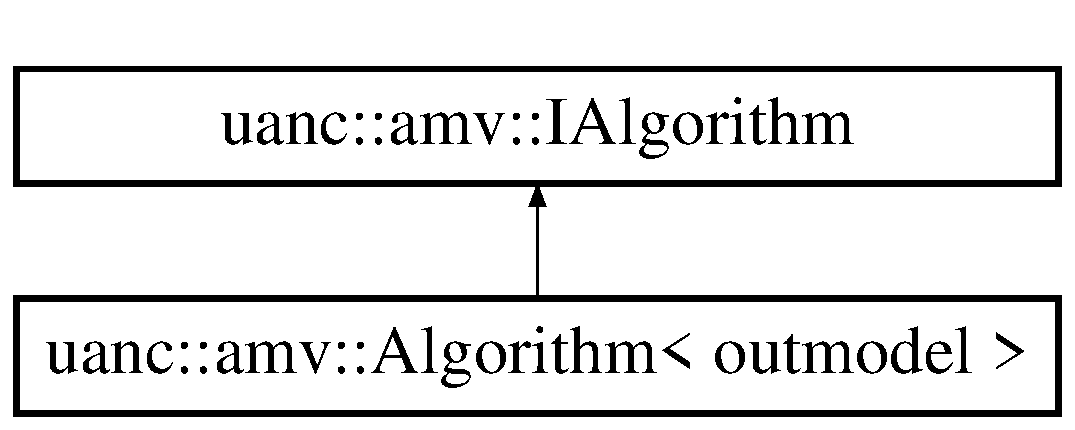
\includegraphics[height=2.000000cm]{classuanc_1_1amv_1_1_algorithm}
\end{center}
\end{figure}
\subsection*{Public Member Functions}
\begin{DoxyCompactItemize}
\item 
void \hyperlink{classuanc_1_1amv_1_1_algorithm_ab85377888f8a0a242803e8ec0dc31db6}{fill\+View} () final
\begin{DoxyCompactList}\small\item\em Fills the view with the data. \end{DoxyCompactList}\item 
\hyperlink{classuanc_1_1amv_1_1_i_algorithm_view}{I\+Algorithm\+View} $\ast$ \hyperlink{classuanc_1_1amv_1_1_algorithm_af0fb55f30a278f0f44427ff690c96fc7}{get\+View} () final
\begin{DoxyCompactList}\small\item\em Gets a reference to the associated view. \end{DoxyCompactList}\item 
void \hyperlink{classuanc_1_1amv_1_1_algorithm_a0af524c2f170204c5c60b2561f286570}{process} (std\+::shared\+\_\+ptr$<$ \hyperlink{classuanc_1_1amv_1_1_inverted_model}{uanc\+::amv\+::\+Inverted\+Model} $>$ input) final
\begin{DoxyCompactList}\small\item\em Processes the input signal model. \end{DoxyCompactList}\end{DoxyCompactItemize}
\subsection*{Protected Member Functions}
\begin{DoxyCompactItemize}
\item 
virtual std\+::shared\+\_\+ptr$<$ outmodel $>$ \hyperlink{classuanc_1_1amv_1_1_algorithm_a3a0bd5e6e8cc1a3f9bd9d9b384e121b5}{execute} (std\+::shared\+\_\+ptr$<$ \hyperlink{classuanc_1_1amv_1_1_inverted_model}{uanc\+::amv\+::\+Inverted\+Model} $>$ input)=0
\begin{DoxyCompactList}\small\item\em Executed an algorithm with the given input model. \end{DoxyCompactList}\item 
virtual \hyperlink{classuanc_1_1amv_1_1_algorithm_view}{Algorithm\+View}$<$ outmodel $>$ $\ast$ \hyperlink{classuanc_1_1amv_1_1_algorithm_af5561072283ed19634893263c95a4b6e}{construct\+View} ()=0
\begin{DoxyCompactList}\small\item\em Constructs a view, which can handle the outmode of the algorithm. \end{DoxyCompactList}\end{DoxyCompactItemize}


\subsection{Detailed Description}
\subsubsection*{template$<$class outmodel$>$\\*
class uanc\+::amv\+::\+Algorithm$<$ outmodel $>$}

This is an algorithm used for defining more specific algorithms. 

This class has to be inherited by any algorithm to be used inside the application. It knows which model the algorithm outputs to define a consistent interface.


\begin{DoxyTemplParams}{Template Parameters}
{\em outmodel} & This is the model generated by the algorithm. Has to be derived from \hyperlink{classuanc_1_1amv_1_1_signal_model}{Signal\+Model}. \\
\hline
\end{DoxyTemplParams}


\subsection{Member Function Documentation}
\index{uanc\+::amv\+::\+Algorithm@{uanc\+::amv\+::\+Algorithm}!construct\+View@{construct\+View}}
\index{construct\+View@{construct\+View}!uanc\+::amv\+::\+Algorithm@{uanc\+::amv\+::\+Algorithm}}
\subsubsection[{\texorpdfstring{construct\+View()=0}{constructView()=0}}]{\setlength{\rightskip}{0pt plus 5cm}template$<$class outmodel$>$ virtual {\bf Algorithm\+View}$<$outmodel$>$$\ast$ {\bf uanc\+::amv\+::\+Algorithm}$<$ outmodel $>$\+::construct\+View (
\begin{DoxyParamCaption}
{}
\end{DoxyParamCaption}
)\hspace{0.3cm}{\ttfamily [protected]}, {\ttfamily [pure virtual]}}\hypertarget{classuanc_1_1amv_1_1_algorithm_af5561072283ed19634893263c95a4b6e}{}\label{classuanc_1_1amv_1_1_algorithm_af5561072283ed19634893263c95a4b6e}


Constructs a view, which can handle the outmode of the algorithm. 

The view should be created inside of this function. Remember, that the view has to be able, to deal with the template parameterized data model of the algorithm.

\begin{DoxyReturn}{Returns}
The created view. 
\end{DoxyReturn}


Implemented in \hyperlink{classuanc_1_1amv_1_1anc_1_1algorithm_1_1_inverse_f_f_t_algorithm_ae2e62b5fc9ef0a7173d86078d5133009}{uanc\+::amv\+::anc\+::algorithm\+::\+Inverse\+F\+F\+T\+Algorithm}, \hyperlink{classuanc_1_1amv_1_1signal_1_1algorithm_1_1_f_f_t_transformation_algorithm_aec3ff4f92dfabd6e2bce66a10ab7b569}{uanc\+::amv\+::signal\+::algorithm\+::\+F\+F\+T\+Transformation\+Algorithm}, \hyperlink{classuanc_1_1amv_1_1anc_1_1algorithm_1_1_spline_interpolation_a93fd1b1f3ac140863f53464eea2820f3}{uanc\+::amv\+::anc\+::algorithm\+::\+Spline\+Interpolation}, \hyperlink{classuanc_1_1amv_1_1anc_1_1algorithm_1_1_inverse_direct_algorithm_ad470192f0ae1042f16750a9181cb61c0}{uanc\+::amv\+::anc\+::algorithm\+::\+Inverse\+Direct\+Algorithm}, \hyperlink{classuanc_1_1amv_1_1anc_1_1algorithm_1_1_linear_extrapolation_a5cd4a27f8c92ab3f95f59cc8be260161}{uanc\+::amv\+::anc\+::algorithm\+::\+Linear\+Extrapolation}, \hyperlink{classuanc_1_1amv_1_1signal_1_1algorithm_1_1_spectrogram_transformation_algorithm_aa36e723764a73225f490cf6baf693a21}{uanc\+::amv\+::signal\+::algorithm\+::\+Spectrogram\+Transformation\+Algorithm}, and \hyperlink{classuanc_1_1amv_1_1signal_1_1algorithm_1_1_identity_transformation_algorithm_a76e6380fcbcef86de4b5aa1fd7f4b77d}{uanc\+::amv\+::signal\+::algorithm\+::\+Identity\+Transformation\+Algorithm}.

\index{uanc\+::amv\+::\+Algorithm@{uanc\+::amv\+::\+Algorithm}!execute@{execute}}
\index{execute@{execute}!uanc\+::amv\+::\+Algorithm@{uanc\+::amv\+::\+Algorithm}}
\subsubsection[{\texorpdfstring{execute(std\+::shared\+\_\+ptr$<$ uanc\+::amv\+::\+Inverted\+Model $>$ input)=0}{execute(std::shared_ptr< uanc::amv::InvertedModel > input)=0}}]{\setlength{\rightskip}{0pt plus 5cm}template$<$class outmodel$>$ virtual std\+::shared\+\_\+ptr$<$outmodel$>$ {\bf uanc\+::amv\+::\+Algorithm}$<$ outmodel $>$\+::execute (
\begin{DoxyParamCaption}
\item[{std\+::shared\+\_\+ptr$<$ {\bf uanc\+::amv\+::\+Inverted\+Model} $>$}]{input}
\end{DoxyParamCaption}
)\hspace{0.3cm}{\ttfamily [protected]}, {\ttfamily [pure virtual]}}\hypertarget{classuanc_1_1amv_1_1_algorithm_a3a0bd5e6e8cc1a3f9bd9d9b384e121b5}{}\label{classuanc_1_1amv_1_1_algorithm_a3a0bd5e6e8cc1a3f9bd9d9b384e121b5}


Executed an algorithm with the given input model. 

This method must be implemented by deriving algorithms, and should execute the algorithm on the input data, generating the correct output model.


\begin{DoxyParams}[1]{Parameters}
\mbox{\tt in}  & {\em input} & The input model of the signal.\\
\hline
\end{DoxyParams}
\begin{DoxyReturn}{Returns}
The created model from the data of the algorithm execution. 
\end{DoxyReturn}


Implemented in \hyperlink{classuanc_1_1amv_1_1signal_1_1algorithm_1_1_signal_transformation_algorithm_a7118b46dcfdadf8648cf927c4bdd70d0}{uanc\+::amv\+::signal\+::algorithm\+::\+Signal\+Transformation\+Algorithm$<$ datamodel, viewmodel $>$}, \hyperlink{classuanc_1_1amv_1_1signal_1_1algorithm_1_1_signal_transformation_algorithm_a7118b46dcfdadf8648cf927c4bdd70d0}{uanc\+::amv\+::signal\+::algorithm\+::\+Signal\+Transformation\+Algorithm$<$ Inverted\+Model $>$}, \hyperlink{classuanc_1_1amv_1_1signal_1_1algorithm_1_1_signal_transformation_algorithm_a7118b46dcfdadf8648cf927c4bdd70d0}{uanc\+::amv\+::signal\+::algorithm\+::\+Signal\+Transformation\+Algorithm$<$ model\+::\+F\+F\+T\+Model $>$}, and \hyperlink{classuanc_1_1amv_1_1signal_1_1algorithm_1_1_signal_transformation_algorithm_a7118b46dcfdadf8648cf927c4bdd70d0}{uanc\+::amv\+::signal\+::algorithm\+::\+Signal\+Transformation\+Algorithm$<$ model\+::\+Spectrogram\+Model $>$}.

\index{uanc\+::amv\+::\+Algorithm@{uanc\+::amv\+::\+Algorithm}!fill\+View@{fill\+View}}
\index{fill\+View@{fill\+View}!uanc\+::amv\+::\+Algorithm@{uanc\+::amv\+::\+Algorithm}}
\subsubsection[{\texorpdfstring{fill\+View() final}{fillView() final}}]{\setlength{\rightskip}{0pt plus 5cm}template$<$class outmodel$>$ void {\bf uanc\+::amv\+::\+Algorithm}$<$ outmodel $>$\+::fill\+View (
\begin{DoxyParamCaption}
{}
\end{DoxyParamCaption}
)\hspace{0.3cm}{\ttfamily [inline]}, {\ttfamily [final]}, {\ttfamily [virtual]}}\hypertarget{classuanc_1_1amv_1_1_algorithm_ab85377888f8a0a242803e8ec0dc31db6}{}\label{classuanc_1_1amv_1_1_algorithm_ab85377888f8a0a242803e8ec0dc31db6}


Fills the view with the data. 

This method fills the view with some data. It basically checks, if the algorithm was already executed and if a view was integrated in the application. If so it plugs the data inside of the view. 

Implements \hyperlink{classuanc_1_1amv_1_1_i_algorithm_a6f71d353db186306f5d4e191f0c15cc4}{uanc\+::amv\+::\+I\+Algorithm}.

\index{uanc\+::amv\+::\+Algorithm@{uanc\+::amv\+::\+Algorithm}!get\+View@{get\+View}}
\index{get\+View@{get\+View}!uanc\+::amv\+::\+Algorithm@{uanc\+::amv\+::\+Algorithm}}
\subsubsection[{\texorpdfstring{get\+View() final}{getView() final}}]{\setlength{\rightskip}{0pt plus 5cm}template$<$class outmodel$>$ {\bf I\+Algorithm\+View}$\ast$ {\bf uanc\+::amv\+::\+Algorithm}$<$ outmodel $>$\+::get\+View (
\begin{DoxyParamCaption}
{}
\end{DoxyParamCaption}
)\hspace{0.3cm}{\ttfamily [inline]}, {\ttfamily [final]}, {\ttfamily [virtual]}}\hypertarget{classuanc_1_1amv_1_1_algorithm_af0fb55f30a278f0f44427ff690c96fc7}{}\label{classuanc_1_1amv_1_1_algorithm_af0fb55f30a278f0f44427ff690c96fc7}


Gets a reference to the associated view. 

This method uses the singleton and the template pattern to create a unique view. The corresponding construct\+View function gets implemented by a leaf class.

\begin{DoxyReturn}{Returns}
The associated view. 
\end{DoxyReturn}


Implements \hyperlink{classuanc_1_1amv_1_1_i_algorithm_ab1806c419a1e73adc149b7fb187d23d7}{uanc\+::amv\+::\+I\+Algorithm}.

\index{uanc\+::amv\+::\+Algorithm@{uanc\+::amv\+::\+Algorithm}!process@{process}}
\index{process@{process}!uanc\+::amv\+::\+Algorithm@{uanc\+::amv\+::\+Algorithm}}
\subsubsection[{\texorpdfstring{process(std\+::shared\+\_\+ptr$<$ uanc\+::amv\+::\+Inverted\+Model $>$ input) final}{process(std::shared_ptr< uanc::amv::InvertedModel > input) final}}]{\setlength{\rightskip}{0pt plus 5cm}template$<$class outmodel$>$ void {\bf uanc\+::amv\+::\+Algorithm}$<$ outmodel $>$\+::process (
\begin{DoxyParamCaption}
\item[{std\+::shared\+\_\+ptr$<$ {\bf uanc\+::amv\+::\+Inverted\+Model} $>$}]{input}
\end{DoxyParamCaption}
)\hspace{0.3cm}{\ttfamily [inline]}, {\ttfamily [final]}, {\ttfamily [virtual]}}\hypertarget{classuanc_1_1amv_1_1_algorithm_a0af524c2f170204c5c60b2561f286570}{}\label{classuanc_1_1amv_1_1_algorithm_a0af524c2f170204c5c60b2561f286570}


Processes the input signal model. 

This method processes the signal model passed into this function. It basically ensures that the function gets called only once and that the generated data is saved inside. It measures the time needed for the execution process.


\begin{DoxyParams}[1]{Parameters}
\mbox{\tt in}  & {\em input} & The input model of the signal. \\
\hline
\end{DoxyParams}


Implements \hyperlink{classuanc_1_1amv_1_1_i_algorithm_a14dd1e42a421c48b8874e42933daa0b9}{uanc\+::amv\+::\+I\+Algorithm}.



The documentation for this class was generated from the following file\+:\begin{DoxyCompactItemize}
\item 
/home/kurt/\+Documents/\+Studium/\+Bachelor\+\_\+\+Praktikum/\+U\+A\+N\+C/\+Code/\+U\+A\+N\+C/amv/\hyperlink{_algorithm_8h}{Algorithm.\+h}\end{DoxyCompactItemize}

\hypertarget{classuanc_1_1amv_1_1_algorithm_thread}{}\section{uanc\+:\+:amv\+:\+:Algorithm\+Thread Class Reference}
\label{classuanc_1_1amv_1_1_algorithm_thread}\index{uanc\+::amv\+::\+Algorithm\+Thread@{uanc\+::amv\+::\+Algorithm\+Thread}}


{\ttfamily \#include $<$Algorithm\+Thread.\+h$>$}

Inheritance diagram for uanc\+:\+:amv\+:\+:Algorithm\+Thread\+:\begin{figure}[H]
\begin{center}
\leavevmode
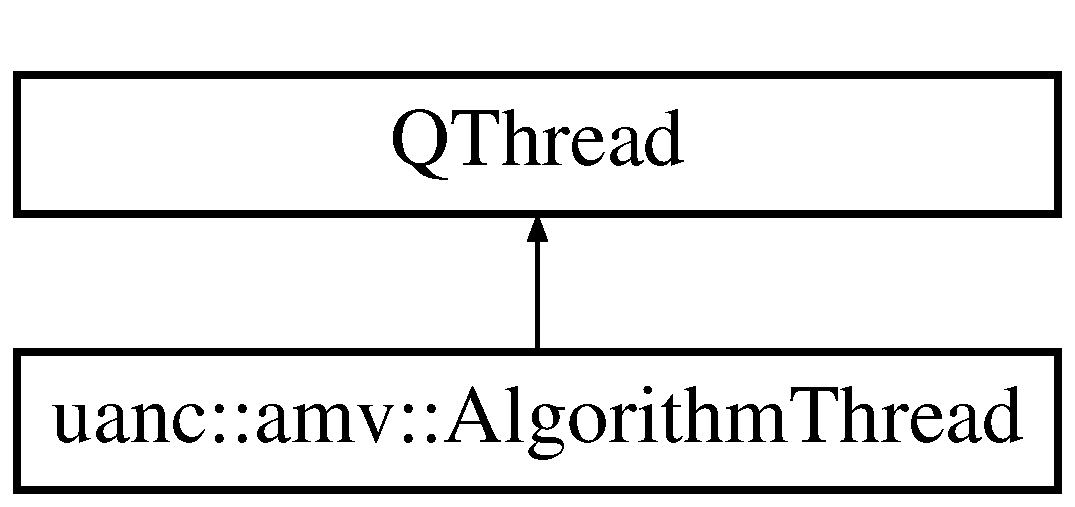
\includegraphics[height=2.000000cm]{classuanc_1_1amv_1_1_algorithm_thread}
\end{center}
\end{figure}
\subsection*{Public Slots}
\begin{DoxyCompactItemize}
\item 
void \hyperlink{classuanc_1_1amv_1_1_algorithm_thread_ac02242d01182f37d1fac4ef594cc4747}{set\+Algorithm} (\hyperlink{classuanc_1_1amv_1_1_i_algorithm}{I\+Algorithm} $\ast$algorithm, std\+::shared\+\_\+ptr$<$ \hyperlink{classuanc_1_1amv_1_1_inverted_model}{Inverted\+Model} $>$ model)
\begin{DoxyCompactList}\small\item\em Can be used to set an algorithm. \end{DoxyCompactList}\end{DoxyCompactItemize}
\subsection*{Signals}
\begin{DoxyCompactItemize}
\item 
void \hyperlink{classuanc_1_1amv_1_1_algorithm_thread_ae4f23094bff85708e4e155828c466112}{algorithm\+Finished} ()
\end{DoxyCompactItemize}
\subsection*{Protected Member Functions}
\begin{DoxyCompactItemize}
\item 
void \hyperlink{classuanc_1_1amv_1_1_algorithm_thread_ad1697895614bad2f2235b1bc9f02323f}{run} () final
\begin{DoxyCompactList}\small\item\em Ru method of this thread. \end{DoxyCompactList}\end{DoxyCompactItemize}


\subsection{Member Function Documentation}
\index{uanc\+::amv\+::\+Algorithm\+Thread@{uanc\+::amv\+::\+Algorithm\+Thread}!algorithm\+Finished@{algorithm\+Finished}}
\index{algorithm\+Finished@{algorithm\+Finished}!uanc\+::amv\+::\+Algorithm\+Thread@{uanc\+::amv\+::\+Algorithm\+Thread}}
\subsubsection[{\texorpdfstring{algorithm\+Finished}{algorithmFinished}}]{\setlength{\rightskip}{0pt plus 5cm}void uanc\+::amv\+::\+Algorithm\+Thread\+::algorithm\+Finished (
\begin{DoxyParamCaption}
{}
\end{DoxyParamCaption}
)\hspace{0.3cm}{\ttfamily [signal]}}\hypertarget{classuanc_1_1amv_1_1_algorithm_thread_ae4f23094bff85708e4e155828c466112}{}\label{classuanc_1_1amv_1_1_algorithm_thread_ae4f23094bff85708e4e155828c466112}
Gets called when the algorithm is finished. \index{uanc\+::amv\+::\+Algorithm\+Thread@{uanc\+::amv\+::\+Algorithm\+Thread}!run@{run}}
\index{run@{run}!uanc\+::amv\+::\+Algorithm\+Thread@{uanc\+::amv\+::\+Algorithm\+Thread}}
\subsubsection[{\texorpdfstring{run() final}{run() final}}]{\setlength{\rightskip}{0pt plus 5cm}void uanc\+::amv\+::\+Algorithm\+Thread\+::run (
\begin{DoxyParamCaption}
{}
\end{DoxyParamCaption}
)\hspace{0.3cm}{\ttfamily [inline]}, {\ttfamily [final]}, {\ttfamily [protected]}}\hypertarget{classuanc_1_1amv_1_1_algorithm_thread_ad1697895614bad2f2235b1bc9f02323f}{}\label{classuanc_1_1amv_1_1_algorithm_thread_ad1697895614bad2f2235b1bc9f02323f}


Ru method of this thread. 

This method does the running of the algorithm. \index{uanc\+::amv\+::\+Algorithm\+Thread@{uanc\+::amv\+::\+Algorithm\+Thread}!set\+Algorithm@{set\+Algorithm}}
\index{set\+Algorithm@{set\+Algorithm}!uanc\+::amv\+::\+Algorithm\+Thread@{uanc\+::amv\+::\+Algorithm\+Thread}}
\subsubsection[{\texorpdfstring{set\+Algorithm}{setAlgorithm}}]{\setlength{\rightskip}{0pt plus 5cm}void uanc\+::amv\+::\+Algorithm\+Thread\+::set\+Algorithm (
\begin{DoxyParamCaption}
\item[{{\bf I\+Algorithm} $\ast$}]{algorithm, }
\item[{std\+::shared\+\_\+ptr$<$ {\bf Inverted\+Model} $>$}]{model}
\end{DoxyParamCaption}
)\hspace{0.3cm}{\ttfamily [inline]}, {\ttfamily [slot]}}\hypertarget{classuanc_1_1amv_1_1_algorithm_thread_ac02242d01182f37d1fac4ef594cc4747}{}\label{classuanc_1_1amv_1_1_algorithm_thread_ac02242d01182f37d1fac4ef594cc4747}


Can be used to set an algorithm. 

This method takes a pointer and saves it internally, to actually know which algorithm to use for the operation.


\begin{DoxyParams}{Parameters}
{\em algorithm} & The \hyperlink{classuanc_1_1amv_1_1_algorithm}{Algorithm} to use. \\
\hline
{\em model} & The Model to invert. \\
\hline
\end{DoxyParams}


The documentation for this class was generated from the following file\+:\begin{DoxyCompactItemize}
\item 
/ext/local/\+University/\+B\+P/\+Git/\+U\+A\+N\+C/\+Code/\+U\+A\+N\+C/amv/\hyperlink{_algorithm_thread_8h}{Algorithm\+Thread.\+h}\end{DoxyCompactItemize}

\hypertarget{classuanc_1_1amv_1_1_algorithm_view}{}\section{uanc\+:\+:amv\+:\+:Algorithm\+View$<$ inmodel $>$ Class Template Reference}
\label{classuanc_1_1amv_1_1_algorithm_view}\index{uanc\+::amv\+::\+Algorithm\+View$<$ inmodel $>$@{uanc\+::amv\+::\+Algorithm\+View$<$ inmodel $>$}}


Basic algorithm associated view.  




{\ttfamily \#include $<$Algorithm\+View.\+h$>$}

Inheritance diagram for uanc\+:\+:amv\+:\+:Algorithm\+View$<$ inmodel $>$\+:\begin{figure}[H]
\begin{center}
\leavevmode
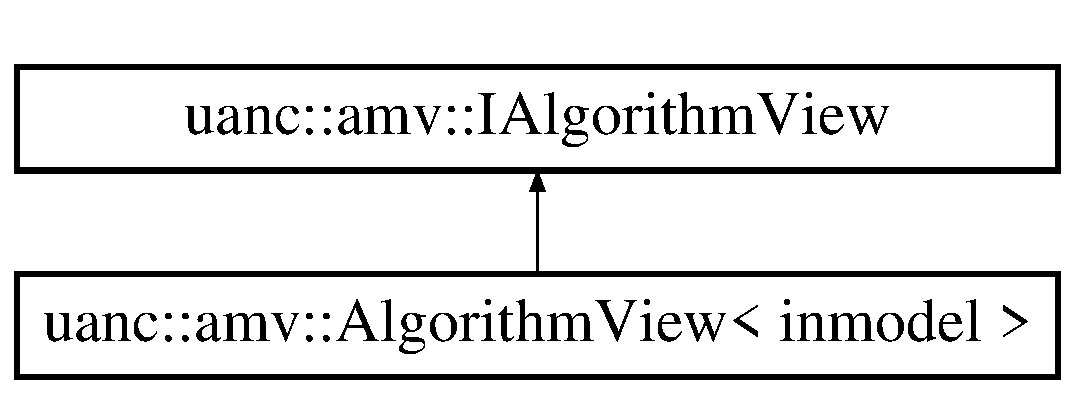
\includegraphics[height=2.000000cm]{classuanc_1_1amv_1_1_algorithm_view}
\end{center}
\end{figure}
\subsection*{Public Member Functions}
\begin{DoxyCompactItemize}
\item 
virtual void \hyperlink{classuanc_1_1amv_1_1_algorithm_view_ad656cf5223a66a942441ee39f44f65a3}{set\+Data} (std\+::shared\+\_\+ptr$<$ inmodel $>$ data)=0
\begin{DoxyCompactList}\small\item\em This method applies the model data. \end{DoxyCompactList}\end{DoxyCompactItemize}


\subsection{Detailed Description}
\subsubsection*{template$<$typename inmodel$>$\\*
class uanc\+::amv\+::\+Algorithm\+View$<$ inmodel $>$}

Basic algorithm associated view. 

This class basically knows the underlying model due to the passed template parameter. This is essential for a cast free use inside of the application. Also it defines what models are applicable.


\begin{DoxyTemplParams}{Template Parameters}
{\em inmodel} & The type of data the model can handle. \\
\hline
\end{DoxyTemplParams}


\subsection{Member Function Documentation}
\index{uanc\+::amv\+::\+Algorithm\+View@{uanc\+::amv\+::\+Algorithm\+View}!set\+Data@{set\+Data}}
\index{set\+Data@{set\+Data}!uanc\+::amv\+::\+Algorithm\+View@{uanc\+::amv\+::\+Algorithm\+View}}
\subsubsection[{\texorpdfstring{set\+Data(std\+::shared\+\_\+ptr$<$ inmodel $>$ data)=0}{setData(std::shared_ptr< inmodel > data)=0}}]{\setlength{\rightskip}{0pt plus 5cm}template$<$typename inmodel$>$ virtual void {\bf uanc\+::amv\+::\+Algorithm\+View}$<$ inmodel $>$\+::set\+Data (
\begin{DoxyParamCaption}
\item[{std\+::shared\+\_\+ptr$<$ inmodel $>$}]{data}
\end{DoxyParamCaption}
)\hspace{0.3cm}{\ttfamily [pure virtual]}}\hypertarget{classuanc_1_1amv_1_1_algorithm_view_ad656cf5223a66a942441ee39f44f65a3}{}\label{classuanc_1_1amv_1_1_algorithm_view_ad656cf5223a66a942441ee39f44f65a3}


This method applies the model data. 

This method simply takes the passed data and places it inside of the view at the appropriate places.


\begin{DoxyParams}{Parameters}
{\em data} & The applied data. \\
\hline
\end{DoxyParams}


Implemented in \hyperlink{classuanc_1_1amv_1_1anc_1_1view_1_1_p_m_view_a6d87a1d7753d1bc76ac7fba5fa03e1d5}{uanc\+::amv\+::anc\+::view\+::\+P\+M\+View}, \hyperlink{classuanc_1_1amv_1_1anc_1_1view_1_1_a_n_c_view_ac9ca194090e787bbe03bb9aec74a7bf4}{uanc\+::amv\+::anc\+::view\+::\+A\+N\+C\+View}, \hyperlink{classuanc_1_1amv_1_1signal_1_1view_1_1_signal_view_a9c7eb492154e043e671549d2c71d94bc}{uanc\+::amv\+::signal\+::view\+::\+Signal\+View}, and \hyperlink{classuanc_1_1amv_1_1signal_1_1view_1_1_heat_view_a0c6ded83c8aefdf05ff1abd8344763df}{uanc\+::amv\+::signal\+::view\+::\+Heat\+View}.



The documentation for this class was generated from the following file\+:\begin{DoxyCompactItemize}
\item 
/ext/local/\+University/\+B\+P/\+Git/\+U\+A\+N\+C/\+Code/\+U\+A\+N\+C/amv/\hyperlink{_algorithm_view_8h}{Algorithm\+View.\+h}\end{DoxyCompactItemize}

\hypertarget{classuanc_1_1amv_1_1anc_1_1algorithm_1_1_a_n_c_algorithm}{}\section{uanc\+:\+:amv\+:\+:anc\+:\+:algorithm\+:\+:A\+N\+C\+Algorithm$<$ datamodel, viewmodel $>$ Class Template Reference}
\label{classuanc_1_1amv_1_1anc_1_1algorithm_1_1_a_n_c_algorithm}\index{uanc\+::amv\+::anc\+::algorithm\+::\+A\+N\+C\+Algorithm$<$ datamodel, viewmodel $>$@{uanc\+::amv\+::anc\+::algorithm\+::\+A\+N\+C\+Algorithm$<$ datamodel, viewmodel $>$}}


Every algorithm used inside has to be derived by this class.  




{\ttfamily \#include $<$A\+N\+C\+Algorithm.\+h$>$}

Inheritance diagram for uanc\+:\+:amv\+:\+:anc\+:\+:algorithm\+:\+:A\+N\+C\+Algorithm$<$ datamodel, viewmodel $>$\+:\begin{figure}[H]
\begin{center}
\leavevmode
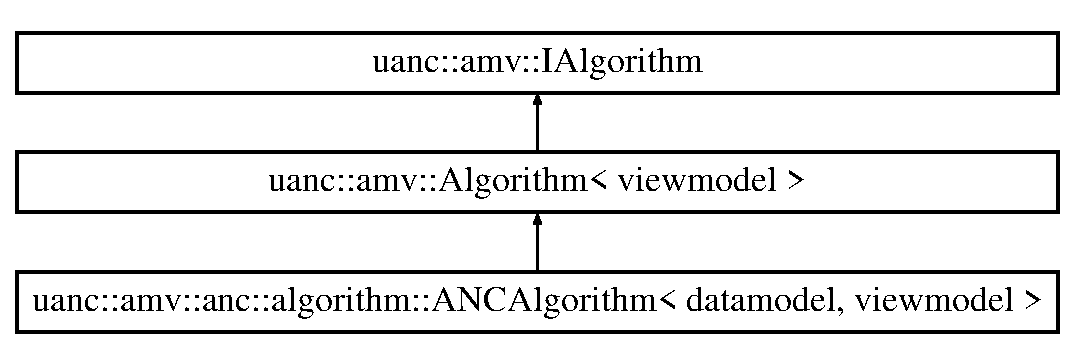
\includegraphics[height=3.000000cm]{classuanc_1_1amv_1_1anc_1_1algorithm_1_1_a_n_c_algorithm}
\end{center}
\end{figure}
\subsection*{Public Member Functions}
\begin{DoxyCompactItemize}
\item 
std\+::shared\+\_\+ptr$<$ datamodel $>$ \hyperlink{classuanc_1_1amv_1_1anc_1_1algorithm_1_1_a_n_c_algorithm_a12ce80f6746cbb440cf771fc6878f7cf}{get\+Model} ()
\begin{DoxyCompactList}\small\item\em Gets a pointer, to access the model of the algorithm. \end{DoxyCompactList}\end{DoxyCompactItemize}
\subsection*{Protected Member Functions}
\begin{DoxyCompactItemize}
\item 
std\+::shared\+\_\+ptr$<$ viewmodel $>$ \hyperlink{classuanc_1_1amv_1_1anc_1_1algorithm_1_1_a_n_c_algorithm_abe01c94fdf777d5081c54311b45341f8}{execute} (std\+::shared\+\_\+ptr$<$ \hyperlink{classuanc_1_1amv_1_1_inverted_model}{Inverted\+Model} $>$ input) final
\begin{DoxyCompactList}\small\item\em Executed an algorithm with the given input model. \end{DoxyCompactList}\item 
virtual void \hyperlink{classuanc_1_1amv_1_1anc_1_1algorithm_1_1_a_n_c_algorithm_abfdc7f14f7e41e408ee08037a839760d}{invert} (std\+::shared\+\_\+ptr$<$ \hyperlink{classuanc_1_1amv_1_1_inverted_model}{Inverted\+Model} $>$ input)=0
\begin{DoxyCompactList}\small\item\em Inverts the input signal. \end{DoxyCompactList}\end{DoxyCompactItemize}


\subsection{Detailed Description}
\subsubsection*{template$<$typename datamodel, typename viewmodel = datamodel$>$\\*
class uanc\+::amv\+::anc\+::algorithm\+::\+A\+N\+C\+Algorithm$<$ datamodel, viewmodel $>$}

Every algorithm used inside has to be derived by this class. 

This represents an \hyperlink{classuanc_1_1amv_1_1anc_1_1algorithm_1_1_a_n_c_algorithm}{A\+N\+C\+Algorithm}. So every inverting algorithm has to be derived by this. In addition one can specify the data model and the view model. If you want to use only a subset of the data you can specify a view model which is actually a parent of the data model. If there is no view model supplied, they will be handled, as if they are the same


\begin{DoxyTemplParams}{Template Parameters}
{\em datamodel} & The data model to use, has to be inherited from viewmodel \\
\hline
{\em viewmodel} & The view model to use, has to be inherited from A\+N\+C\+Model \\
\hline
\end{DoxyTemplParams}


\subsection{Member Function Documentation}
\index{uanc\+::amv\+::anc\+::algorithm\+::\+A\+N\+C\+Algorithm@{uanc\+::amv\+::anc\+::algorithm\+::\+A\+N\+C\+Algorithm}!execute@{execute}}
\index{execute@{execute}!uanc\+::amv\+::anc\+::algorithm\+::\+A\+N\+C\+Algorithm@{uanc\+::amv\+::anc\+::algorithm\+::\+A\+N\+C\+Algorithm}}
\subsubsection[{\texorpdfstring{execute(std\+::shared\+\_\+ptr$<$ Inverted\+Model $>$ input) final}{execute(std::shared_ptr< InvertedModel > input) final}}]{\setlength{\rightskip}{0pt plus 5cm}template$<$typename datamodel, typename viewmodel = datamodel$>$ std\+::shared\+\_\+ptr$<$viewmodel$>$ {\bf uanc\+::amv\+::anc\+::algorithm\+::\+A\+N\+C\+Algorithm}$<$ datamodel, viewmodel $>$\+::execute (
\begin{DoxyParamCaption}
\item[{std\+::shared\+\_\+ptr$<$ {\bf Inverted\+Model} $>$}]{input}
\end{DoxyParamCaption}
)\hspace{0.3cm}{\ttfamily [inline]}, {\ttfamily [final]}, {\ttfamily [protected]}}\hypertarget{classuanc_1_1amv_1_1anc_1_1algorithm_1_1_a_n_c_algorithm_abe01c94fdf777d5081c54311b45341f8}{}\label{classuanc_1_1amv_1_1anc_1_1algorithm_1_1_a_n_c_algorithm_abe01c94fdf777d5081c54311b45341f8}


Executed an algorithm with the given input model. 

This method first all gets an empty model from the deriving class. Afterwards it inverts the signal and passed back the model, which was created during the execution stage.


\begin{DoxyParams}[1]{Parameters}
\mbox{\tt in}  & {\em input} & The input model of the signal.\\
\hline
\end{DoxyParams}
\begin{DoxyReturn}{Returns}
The created model from the data of the inversion. 
\end{DoxyReturn}
\index{uanc\+::amv\+::anc\+::algorithm\+::\+A\+N\+C\+Algorithm@{uanc\+::amv\+::anc\+::algorithm\+::\+A\+N\+C\+Algorithm}!get\+Model@{get\+Model}}
\index{get\+Model@{get\+Model}!uanc\+::amv\+::anc\+::algorithm\+::\+A\+N\+C\+Algorithm@{uanc\+::amv\+::anc\+::algorithm\+::\+A\+N\+C\+Algorithm}}
\subsubsection[{\texorpdfstring{get\+Model()}{getModel()}}]{\setlength{\rightskip}{0pt plus 5cm}template$<$typename datamodel, typename viewmodel = datamodel$>$ std\+::shared\+\_\+ptr$<$datamodel$>$ {\bf uanc\+::amv\+::anc\+::algorithm\+::\+A\+N\+C\+Algorithm}$<$ datamodel, viewmodel $>$\+::get\+Model (
\begin{DoxyParamCaption}
{}
\end{DoxyParamCaption}
)\hspace{0.3cm}{\ttfamily [inline]}}\hypertarget{classuanc_1_1amv_1_1anc_1_1algorithm_1_1_a_n_c_algorithm_a12ce80f6746cbb440cf771fc6878f7cf}{}\label{classuanc_1_1amv_1_1anc_1_1algorithm_1_1_a_n_c_algorithm_a12ce80f6746cbb440cf771fc6878f7cf}


Gets a pointer, to access the model of the algorithm. 

Getter for the model used inside of the algorithm. This pointer can be modified by deriving classes to manipulate the model.

\begin{DoxyReturn}{Returns}
The pointer to the data model stored inside. 
\end{DoxyReturn}
\index{uanc\+::amv\+::anc\+::algorithm\+::\+A\+N\+C\+Algorithm@{uanc\+::amv\+::anc\+::algorithm\+::\+A\+N\+C\+Algorithm}!invert@{invert}}
\index{invert@{invert}!uanc\+::amv\+::anc\+::algorithm\+::\+A\+N\+C\+Algorithm@{uanc\+::amv\+::anc\+::algorithm\+::\+A\+N\+C\+Algorithm}}
\subsubsection[{\texorpdfstring{invert(std\+::shared\+\_\+ptr$<$ Inverted\+Model $>$ input)=0}{invert(std::shared_ptr< InvertedModel > input)=0}}]{\setlength{\rightskip}{0pt plus 5cm}template$<$typename datamodel, typename viewmodel = datamodel$>$ virtual void {\bf uanc\+::amv\+::anc\+::algorithm\+::\+A\+N\+C\+Algorithm}$<$ datamodel, viewmodel $>$\+::invert (
\begin{DoxyParamCaption}
\item[{std\+::shared\+\_\+ptr$<$ {\bf Inverted\+Model} $>$}]{input}
\end{DoxyParamCaption}
)\hspace{0.3cm}{\ttfamily [protected]}, {\ttfamily [pure virtual]}}\hypertarget{classuanc_1_1amv_1_1anc_1_1algorithm_1_1_a_n_c_algorithm_abfdc7f14f7e41e408ee08037a839760d}{}\label{classuanc_1_1amv_1_1anc_1_1algorithm_1_1_a_n_c_algorithm_abfdc7f14f7e41e408ee08037a839760d}


Inverts the input signal. 

This is actually the heart of an A\+NC algorithm inside of this application. It takes an input model and processes it. Besides it should save its data inside the model using \hyperlink{classuanc_1_1amv_1_1anc_1_1algorithm_1_1_a_n_c_algorithm_a12ce80f6746cbb440cf771fc6878f7cf}{get\+Model()}.


\begin{DoxyParams}{Parameters}
{\em input} & The input model containing the original signal. \\
\hline
\end{DoxyParams}


Implemented in \hyperlink{classuanc_1_1amv_1_1anc_1_1algorithm_1_1_inverse_f_f_t_algorithm_a75d38b5ce03bca80a856dfa257f590a4}{uanc\+::amv\+::anc\+::algorithm\+::\+Inverse\+F\+F\+T\+Algorithm}, \hyperlink{classuanc_1_1amv_1_1anc_1_1algorithm_1_1_inverse_direct_algorithm_a4bd1bdcd128aee1f608be51660528954}{uanc\+::amv\+::anc\+::algorithm\+::\+Inverse\+Direct\+Algorithm}, \hyperlink{classuanc_1_1amv_1_1anc_1_1algorithm_1_1_spline_interpolation_a60dcdd5acbba6fee64cf228485b81523}{uanc\+::amv\+::anc\+::algorithm\+::\+Spline\+Interpolation}, and \hyperlink{classuanc_1_1amv_1_1anc_1_1algorithm_1_1_linear_extrapolation_aafb6717c9cb632241b10875630970388}{uanc\+::amv\+::anc\+::algorithm\+::\+Linear\+Extrapolation}.



The documentation for this class was generated from the following file\+:\begin{DoxyCompactItemize}
\item 
/home/kurt/\+Documents/\+Studium/\+Bachelor\+\_\+\+Praktikum/\+U\+A\+N\+C/\+Code/\+U\+A\+N\+C/amv/anc/algorithm/\hyperlink{_a_n_c_algorithm_8h}{A\+N\+C\+Algorithm.\+h}\end{DoxyCompactItemize}

\hypertarget{classuanc_1_1amv_1_1anc_1_1_a_n_c_algorithm_register}{}\section{uanc\+:\+:amv\+:\+:anc\+:\+:A\+N\+C\+Algorithm\+Register Class Reference}
\label{classuanc_1_1amv_1_1anc_1_1_a_n_c_algorithm_register}\index{uanc\+::amv\+::anc\+::\+A\+N\+C\+Algorithm\+Register@{uanc\+::amv\+::anc\+::\+A\+N\+C\+Algorithm\+Register}}


This class is used to retain a list of all algorithms.  




{\ttfamily \#include $<$A\+N\+C\+Algorithm\+Register.\+h$>$}

\subsection*{Static Public Member Functions}
\begin{DoxyCompactItemize}
\item 
static std\+::shared\+\_\+ptr$<$ std\+::vector$<$ \hyperlink{classuanc_1_1amv_1_1_i_algorithm}{uanc\+::amv\+::\+I\+Algorithm} $\ast$ $>$ $>$ \hyperlink{classuanc_1_1amv_1_1anc_1_1_a_n_c_algorithm_register_ad3df250b009b0d6564fcfc8872e21356}{get\+Algorithms} ()
\begin{DoxyCompactList}\small\item\em Supply all registered algorithms. \end{DoxyCompactList}\end{DoxyCompactItemize}


\subsection{Detailed Description}
This class is used to retain a list of all algorithms. 

This class represents the extendability point for all algorithms. If you have implemented an algorithm simply register it inside of this class and it will automatically be integrated in the application. 

\subsection{Member Function Documentation}
\index{uanc\+::amv\+::anc\+::\+A\+N\+C\+Algorithm\+Register@{uanc\+::amv\+::anc\+::\+A\+N\+C\+Algorithm\+Register}!get\+Algorithms@{get\+Algorithms}}
\index{get\+Algorithms@{get\+Algorithms}!uanc\+::amv\+::anc\+::\+A\+N\+C\+Algorithm\+Register@{uanc\+::amv\+::anc\+::\+A\+N\+C\+Algorithm\+Register}}
\subsubsection[{\texorpdfstring{get\+Algorithms()}{getAlgorithms()}}]{\setlength{\rightskip}{0pt plus 5cm}static std\+::shared\+\_\+ptr$<$std\+::vector$<${\bf uanc\+::amv\+::\+I\+Algorithm} $\ast$$>$ $>$ uanc\+::amv\+::anc\+::\+A\+N\+C\+Algorithm\+Register\+::get\+Algorithms (
\begin{DoxyParamCaption}
{}
\end{DoxyParamCaption}
)\hspace{0.3cm}{\ttfamily [inline]}, {\ttfamily [static]}}\hypertarget{classuanc_1_1amv_1_1anc_1_1_a_n_c_algorithm_register_ad3df250b009b0d6564fcfc8872e21356}{}\label{classuanc_1_1amv_1_1anc_1_1_a_n_c_algorithm_register_ad3df250b009b0d6564fcfc8872e21356}


Supply all registered algorithms. 

This method basically returns a list of all algorithms registered inside of the application. To add you new implemented one, simply add it to the list at the bottom.

\begin{DoxyReturn}{Returns}
A vector containing a prototype of all algorithms. 
\end{DoxyReturn}


The documentation for this class was generated from the following file\+:\begin{DoxyCompactItemize}
\item 
/ext/local/\+University/\+B\+P/\+Git/\+U\+A\+N\+C/\+Code/\+U\+A\+N\+C/amv/anc/\hyperlink{_a_n_c_algorithm_register_8h}{A\+N\+C\+Algorithm\+Register.\+h}\end{DoxyCompactItemize}

\hypertarget{classuanc_1_1amv_1_1anc_1_1model_1_1_a_n_c_model}{}\section{uanc\+:\+:amv\+:\+:anc\+:\+:model\+:\+:A\+N\+C\+Model Class Reference}
\label{classuanc_1_1amv_1_1anc_1_1model_1_1_a_n_c_model}\index{uanc\+::amv\+::anc\+::model\+::\+A\+N\+C\+Model@{uanc\+::amv\+::anc\+::model\+::\+A\+N\+C\+Model}}


This is an \hyperlink{classuanc_1_1amv_1_1anc_1_1model_1_1_a_n_c_model}{A\+N\+C\+Model}.  




{\ttfamily \#include $<$A\+N\+C\+Model.\+h$>$}

Inheritance diagram for uanc\+:\+:amv\+:\+:anc\+:\+:model\+:\+:A\+N\+C\+Model\+:\begin{figure}[H]
\begin{center}
\leavevmode
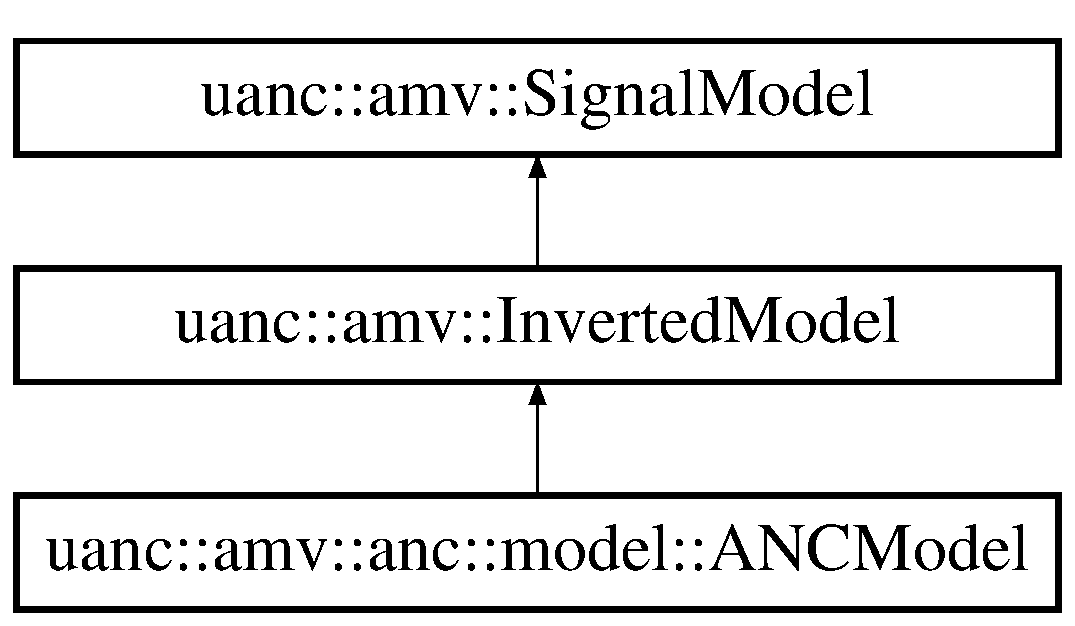
\includegraphics[height=3.000000cm]{classuanc_1_1amv_1_1anc_1_1model_1_1_a_n_c_model}
\end{center}
\end{figure}
\subsection*{Public Attributes}
\begin{DoxyCompactItemize}
\item 
\hyperlink{classuanc_1_1amv_1_1_p_m_register_1_1_performance_measurement_register}{P\+M\+Register\+::\+Performance\+Measurement\+Register} \hyperlink{classuanc_1_1amv_1_1anc_1_1model_1_1_a_n_c_model_a1e7a3078128b1b92eda1e0bbfbfaa610}{default\+Register}
\end{DoxyCompactItemize}


\subsection{Detailed Description}
This is an \hyperlink{classuanc_1_1amv_1_1anc_1_1model_1_1_a_n_c_model}{A\+N\+C\+Model}. 

This model gets derived from the \hyperlink{classuanc_1_1amv_1_1_signal_model}{Signal\+Model}. It adds a field containing the inverted signal to the original signal in \hyperlink{classuanc_1_1amv_1_1_signal_model}{Signal\+Model}. 

\subsection{Member Data Documentation}
\index{uanc\+::amv\+::anc\+::model\+::\+A\+N\+C\+Model@{uanc\+::amv\+::anc\+::model\+::\+A\+N\+C\+Model}!default\+Register@{default\+Register}}
\index{default\+Register@{default\+Register}!uanc\+::amv\+::anc\+::model\+::\+A\+N\+C\+Model@{uanc\+::amv\+::anc\+::model\+::\+A\+N\+C\+Model}}
\subsubsection[{\texorpdfstring{default\+Register}{defaultRegister}}]{\setlength{\rightskip}{0pt plus 5cm}{\bf P\+M\+Register\+::\+Performance\+Measurement\+Register} uanc\+::amv\+::anc\+::model\+::\+A\+N\+C\+Model\+::default\+Register}\hypertarget{classuanc_1_1amv_1_1anc_1_1model_1_1_a_n_c_model_a1e7a3078128b1b92eda1e0bbfbfaa610}{}\label{classuanc_1_1amv_1_1anc_1_1model_1_1_a_n_c_model_a1e7a3078128b1b92eda1e0bbfbfaa610}
This member is the container for default and custom performance measurements. 

The documentation for this class was generated from the following file\+:\begin{DoxyCompactItemize}
\item 
/ext/local/\+University/\+B\+P/\+Git/\+U\+A\+N\+C/\+Code/\+U\+A\+N\+C/amv/anc/model/\hyperlink{_a_n_c_model_8h}{A\+N\+C\+Model.\+h}\end{DoxyCompactItemize}

\hypertarget{classuanc_1_1amv_1_1anc_1_1view_1_1_a_n_c_view}{}\section{uanc\+:\+:amv\+:\+:anc\+:\+:view\+:\+:A\+N\+C\+View Class Reference}
\label{classuanc_1_1amv_1_1anc_1_1view_1_1_a_n_c_view}\index{uanc\+::amv\+::anc\+::view\+::\+A\+N\+C\+View@{uanc\+::amv\+::anc\+::view\+::\+A\+N\+C\+View}}


Represents an \hyperlink{classuanc_1_1amv_1_1anc_1_1view_1_1_a_n_c_view}{A\+N\+C\+View}.  




{\ttfamily \#include $<$A\+N\+C\+View.\+h$>$}

Inheritance diagram for uanc\+:\+:amv\+:\+:anc\+:\+:view\+:\+:A\+N\+C\+View\+:\begin{figure}[H]
\begin{center}
\leavevmode
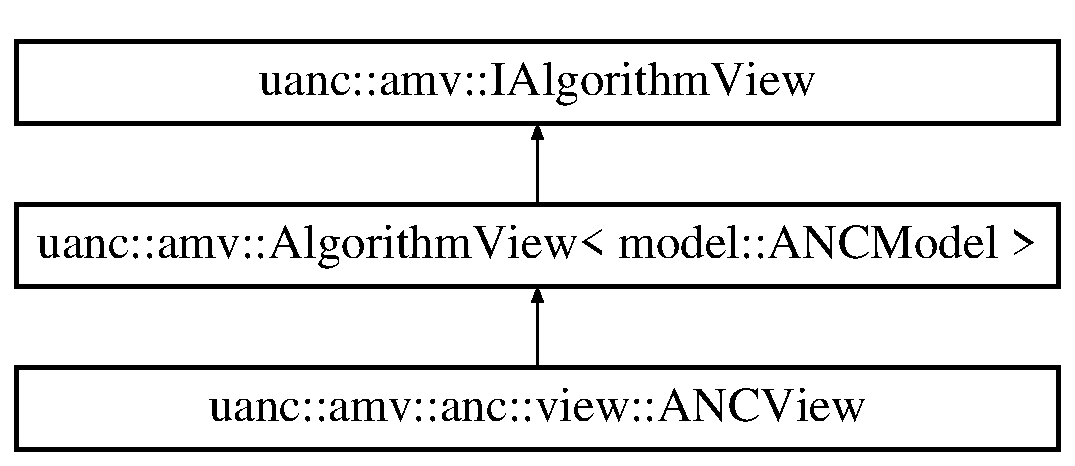
\includegraphics[height=3.000000cm]{classuanc_1_1amv_1_1anc_1_1view_1_1_a_n_c_view}
\end{center}
\end{figure}
\subsection*{Public Member Functions}
\begin{DoxyCompactItemize}
\item 
Q\+Widget $\ast$ \hyperlink{classuanc_1_1amv_1_1anc_1_1view_1_1_a_n_c_view_ab8ad6046c26c2eae15edc82fdbae9aa1}{produce\+Widget} () final
\begin{DoxyCompactList}\small\item\em Gets the complete widget. \end{DoxyCompactList}\item 
void \hyperlink{classuanc_1_1amv_1_1anc_1_1view_1_1_a_n_c_view_ac9ca194090e787bbe03bb9aec74a7bf4}{set\+Data} (std\+::shared\+\_\+ptr$<$ \hyperlink{classuanc_1_1amv_1_1anc_1_1model_1_1_a_n_c_model}{model\+::\+A\+N\+C\+Model} $>$ data) final
\begin{DoxyCompactList}\small\item\em This method applies the model data. \end{DoxyCompactList}\end{DoxyCompactItemize}


\subsection{Detailed Description}
Represents an \hyperlink{classuanc_1_1amv_1_1anc_1_1view_1_1_a_n_c_view}{A\+N\+C\+View}. 

This represents a general \hyperlink{classuanc_1_1amv_1_1anc_1_1view_1_1_a_n_c_view}{A\+N\+C\+View}. It operates on an A\+N\+C\+Model. It only displays a simple plot of the the inverted signal. It is a specialization of the more general \hyperlink{classuanc_1_1amv_1_1_algorithm_view}{Algorithm\+View}. 

\subsection{Member Function Documentation}
\index{uanc\+::amv\+::anc\+::view\+::\+A\+N\+C\+View@{uanc\+::amv\+::anc\+::view\+::\+A\+N\+C\+View}!produce\+Widget@{produce\+Widget}}
\index{produce\+Widget@{produce\+Widget}!uanc\+::amv\+::anc\+::view\+::\+A\+N\+C\+View@{uanc\+::amv\+::anc\+::view\+::\+A\+N\+C\+View}}
\subsubsection[{\texorpdfstring{produce\+Widget() final}{produceWidget() final}}]{\setlength{\rightskip}{0pt plus 5cm}Q\+Widget $\ast$ uanc\+::amv\+::anc\+::view\+::\+A\+N\+C\+View\+::produce\+Widget (
\begin{DoxyParamCaption}
{}
\end{DoxyParamCaption}
)\hspace{0.3cm}{\ttfamily [final]}, {\ttfamily [virtual]}}\hypertarget{classuanc_1_1amv_1_1anc_1_1view_1_1_a_n_c_view_ab8ad6046c26c2eae15edc82fdbae9aa1}{}\label{classuanc_1_1amv_1_1anc_1_1view_1_1_a_n_c_view_ab8ad6046c26c2eae15edc82fdbae9aa1}


Gets the complete widget. 

This function is used to retrieve the widget from the view. It gets used for integration the main application. It creates a Plotwidget inside of a Q\+Widget and passes this back.

\begin{DoxyReturn}{Returns}
The created widget.
\end{DoxyReturn}
This function is used to retrieve the widget from the view. It gets used for integration the main application. It creates a Plotwidget inside of a Q\+Widget and passes this back. Uses the singleton pattern to ensure the unique creation of the widget.

\begin{DoxyReturn}{Returns}
The created widget. 
\end{DoxyReturn}


Implements \hyperlink{classuanc_1_1amv_1_1_i_algorithm_view_ab9d06a0b43db57244868f10dae8e09e5}{uanc\+::amv\+::\+I\+Algorithm\+View}.

\index{uanc\+::amv\+::anc\+::view\+::\+A\+N\+C\+View@{uanc\+::amv\+::anc\+::view\+::\+A\+N\+C\+View}!set\+Data@{set\+Data}}
\index{set\+Data@{set\+Data}!uanc\+::amv\+::anc\+::view\+::\+A\+N\+C\+View@{uanc\+::amv\+::anc\+::view\+::\+A\+N\+C\+View}}
\subsubsection[{\texorpdfstring{set\+Data(std\+::shared\+\_\+ptr$<$ model\+::\+A\+N\+C\+Model $>$ data) final}{setData(std::shared_ptr< model::ANCModel > data) final}}]{\setlength{\rightskip}{0pt plus 5cm}void uanc\+::amv\+::anc\+::view\+::\+A\+N\+C\+View\+::set\+Data (
\begin{DoxyParamCaption}
\item[{std\+::shared\+\_\+ptr$<$ {\bf model\+::\+A\+N\+C\+Model} $>$}]{data}
\end{DoxyParamCaption}
)\hspace{0.3cm}{\ttfamily [final]}, {\ttfamily [virtual]}}\hypertarget{classuanc_1_1amv_1_1anc_1_1view_1_1_a_n_c_view_ac9ca194090e787bbe03bb9aec74a7bf4}{}\label{classuanc_1_1amv_1_1anc_1_1view_1_1_a_n_c_view_ac9ca194090e787bbe03bb9aec74a7bf4}


This method applies the model data. 

This method simply takes the passed data and places it inside of the view at the appropriate places.


\begin{DoxyParams}{Parameters}
{\em data} & The applied data. \\
\hline
\end{DoxyParams}


Implements \hyperlink{classuanc_1_1amv_1_1_algorithm_view_ad656cf5223a66a942441ee39f44f65a3}{uanc\+::amv\+::\+Algorithm\+View$<$ model\+::\+A\+N\+C\+Model $>$}.



The documentation for this class was generated from the following files\+:\begin{DoxyCompactItemize}
\item 
/home/kurt/\+Documents/\+Studium/\+Bachelor\+\_\+\+Praktikum/\+U\+A\+N\+C/\+Code/\+U\+A\+N\+C/amv/anc/view/\hyperlink{_a_n_c_view_8h}{A\+N\+C\+View.\+h}\item 
/home/kurt/\+Documents/\+Studium/\+Bachelor\+\_\+\+Praktikum/\+U\+A\+N\+C/\+Code/\+U\+A\+N\+C/amv/anc/view/\hyperlink{_a_n_c_view_8cpp}{A\+N\+C\+View.\+cpp}\end{DoxyCompactItemize}

\hypertarget{classuanc_1_1gui_1_1_control}{}\section{uanc\+:\+:gui\+:\+:Control Class Reference}
\label{classuanc_1_1gui_1_1_control}\index{uanc\+::gui\+::\+Control@{uanc\+::gui\+::\+Control}}


{\ttfamily \#include $<$Control.\+h$>$}

Inheritance diagram for uanc\+:\+:gui\+:\+:Control\+:\begin{figure}[H]
\begin{center}
\leavevmode
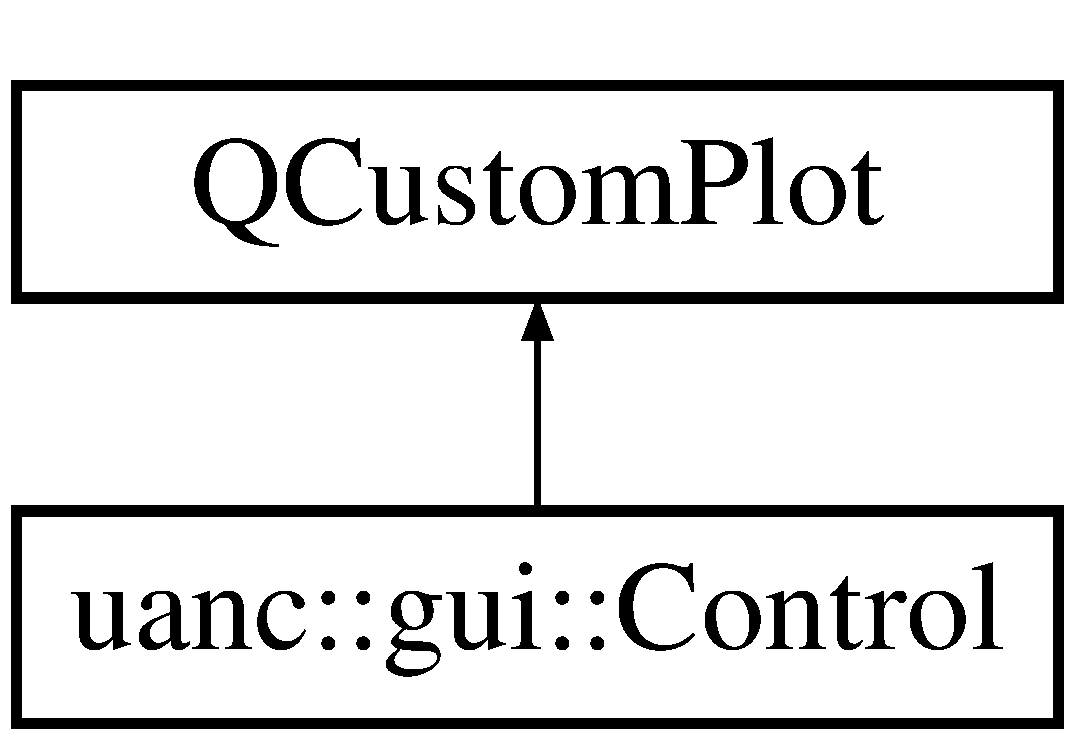
\includegraphics[height=2.000000cm]{classuanc_1_1gui_1_1_control}
\end{center}
\end{figure}
\subsection*{Public Member Functions}
\begin{DoxyCompactItemize}
\item 
\hyperlink{classuanc_1_1gui_1_1_control_a4ad4c4c3eafb8b794dc532f7c92834ec}{Control} (\hyperlink{classuanc_1_1gui_1_1_plot_widget}{Plot\+Widget} $\ast$parent)
\begin{DoxyCompactList}\small\item\em Constructor of \hyperlink{classuanc_1_1gui_1_1_control}{Control} class. \end{DoxyCompactList}\item 
void \hyperlink{classuanc_1_1gui_1_1_control_af4b37736f5e75f13bea8579affeb960c}{set\+Data} (Q\+C\+P\+Graph\+Data\+Container $\ast$data, double max\+Data\+Value, double min\+Data\+Value)
\begin{DoxyCompactList}\small\item\em rescales the axes for the data rescales the axis to a given minimum and maximum of a data \end{DoxyCompactList}\item 
void \hyperlink{classuanc_1_1gui_1_1_control_a621e6bef8d7ade46bbf81e36690618af}{update\+Nav\+Box} (Q\+C\+P\+Range signal\+Zoom\+Range)
\begin{DoxyCompactList}\small\item\em updates navigation box updates navigation box after zoom \end{DoxyCompactList}\item 
double \hyperlink{classuanc_1_1gui_1_1_control_a219dd654ffa8fb96944defe6cf167401}{get\+Box\+Left} ()
\item 
double \hyperlink{classuanc_1_1gui_1_1_control_a4ccfd10312d76eea24f7991632692b59}{get\+Box\+Right} ()
\end{DoxyCompactItemize}


\subsection{Constructor \& Destructor Documentation}
\index{uanc\+::gui\+::\+Control@{uanc\+::gui\+::\+Control}!Control@{Control}}
\index{Control@{Control}!uanc\+::gui\+::\+Control@{uanc\+::gui\+::\+Control}}
\subsubsection[{\texorpdfstring{Control(\+Plot\+Widget $\ast$parent)}{Control(PlotWidget *parent)}}]{\setlength{\rightskip}{0pt plus 5cm}uanc\+::gui\+::\+Control\+::\+Control (
\begin{DoxyParamCaption}
\item[{{\bf Plot\+Widget} $\ast$}]{parent}
\end{DoxyParamCaption}
)}\hypertarget{classuanc_1_1gui_1_1_control_a4ad4c4c3eafb8b794dc532f7c92834ec}{}\label{classuanc_1_1gui_1_1_control_a4ad4c4c3eafb8b794dc532f7c92834ec}


Constructor of \hyperlink{classuanc_1_1gui_1_1_control}{Control} class. 


\begin{DoxyParams}{Parameters}
{\em parent} & this is the parent widget \\
\hline
\end{DoxyParams}


\subsection{Member Function Documentation}
\index{uanc\+::gui\+::\+Control@{uanc\+::gui\+::\+Control}!get\+Box\+Left@{get\+Box\+Left}}
\index{get\+Box\+Left@{get\+Box\+Left}!uanc\+::gui\+::\+Control@{uanc\+::gui\+::\+Control}}
\subsubsection[{\texorpdfstring{get\+Box\+Left()}{getBoxLeft()}}]{\setlength{\rightskip}{0pt plus 5cm}double uanc\+::gui\+::\+Control\+::get\+Box\+Left (
\begin{DoxyParamCaption}
{}
\end{DoxyParamCaption}
)}\hypertarget{classuanc_1_1gui_1_1_control_a219dd654ffa8fb96944defe6cf167401}{}\label{classuanc_1_1gui_1_1_control_a219dd654ffa8fb96944defe6cf167401}
retrieve the left box \index{uanc\+::gui\+::\+Control@{uanc\+::gui\+::\+Control}!get\+Box\+Right@{get\+Box\+Right}}
\index{get\+Box\+Right@{get\+Box\+Right}!uanc\+::gui\+::\+Control@{uanc\+::gui\+::\+Control}}
\subsubsection[{\texorpdfstring{get\+Box\+Right()}{getBoxRight()}}]{\setlength{\rightskip}{0pt plus 5cm}double uanc\+::gui\+::\+Control\+::get\+Box\+Right (
\begin{DoxyParamCaption}
{}
\end{DoxyParamCaption}
)}\hypertarget{classuanc_1_1gui_1_1_control_a4ccfd10312d76eea24f7991632692b59}{}\label{classuanc_1_1gui_1_1_control_a4ccfd10312d76eea24f7991632692b59}
retrieve the right box \index{uanc\+::gui\+::\+Control@{uanc\+::gui\+::\+Control}!set\+Data@{set\+Data}}
\index{set\+Data@{set\+Data}!uanc\+::gui\+::\+Control@{uanc\+::gui\+::\+Control}}
\subsubsection[{\texorpdfstring{set\+Data(\+Q\+C\+P\+Graph\+Data\+Container $\ast$data, double max\+Data\+Value, double min\+Data\+Value)}{setData(QCPGraphDataContainer *data, double maxDataValue, double minDataValue)}}]{\setlength{\rightskip}{0pt plus 5cm}void uanc\+::gui\+::\+Control\+::set\+Data (
\begin{DoxyParamCaption}
\item[{Q\+C\+P\+Graph\+Data\+Container $\ast$}]{data, }
\item[{double}]{max\+Data\+Value, }
\item[{double}]{min\+Data\+Value}
\end{DoxyParamCaption}
)}\hypertarget{classuanc_1_1gui_1_1_control_af4b37736f5e75f13bea8579affeb960c}{}\label{classuanc_1_1gui_1_1_control_af4b37736f5e75f13bea8579affeb960c}


rescales the axes for the data rescales the axis to a given minimum and maximum of a data 


\begin{DoxyParams}{Parameters}
{\em $\ast$data} & this is the data that has to be rescaled \\
\hline
{\em max\+Data\+Value} & this is the maximum value in the data \\
\hline
{\em min\+Data\+Value} & this is the minimum value in the data \\
\hline
\end{DoxyParams}
\index{uanc\+::gui\+::\+Control@{uanc\+::gui\+::\+Control}!update\+Nav\+Box@{update\+Nav\+Box}}
\index{update\+Nav\+Box@{update\+Nav\+Box}!uanc\+::gui\+::\+Control@{uanc\+::gui\+::\+Control}}
\subsubsection[{\texorpdfstring{update\+Nav\+Box(\+Q\+C\+P\+Range signal\+Zoom\+Range)}{updateNavBox(QCPRange signalZoomRange)}}]{\setlength{\rightskip}{0pt plus 5cm}void uanc\+::gui\+::\+Control\+::update\+Nav\+Box (
\begin{DoxyParamCaption}
\item[{Q\+C\+P\+Range}]{signal\+Zoom\+Range}
\end{DoxyParamCaption}
)}\hypertarget{classuanc_1_1gui_1_1_control_a621e6bef8d7ade46bbf81e36690618af}{}\label{classuanc_1_1gui_1_1_control_a621e6bef8d7ade46bbf81e36690618af}


updates navigation box updates navigation box after zoom 


\begin{DoxyParams}{Parameters}
{\em signal\+Zoom\+Range} & the range of the zoomed signal \\
\hline
\end{DoxyParams}


The documentation for this class was generated from the following files\+:\begin{DoxyCompactItemize}
\item 
/ext/local/\+University/\+B\+P/\+Git/\+U\+A\+N\+C/\+Code/\+U\+A\+N\+C/gui/\hyperlink{_control_8h}{Control.\+h}\item 
/ext/local/\+University/\+B\+P/\+Git/\+U\+A\+N\+C/\+Code/\+U\+A\+N\+C/gui/\hyperlink{_control_8cpp}{Control.\+cpp}\end{DoxyCompactItemize}

\hypertarget{classuanc_1_1util_1_1_dialog_util}{}\section{uanc\+:\+:util\+:\+:Dialog\+Util Class Reference}
\label{classuanc_1_1util_1_1_dialog_util}\index{uanc\+::util\+::\+Dialog\+Util@{uanc\+::util\+::\+Dialog\+Util}}


This class can be used to access various dialogs.  




{\ttfamily \#include $<$Dialog\+Util.\+h$>$}

\subsection*{Public Member Functions}
\begin{DoxyCompactItemize}
\item 
\hyperlink{classuanc_1_1util_1_1_dialog_util_a1d190a4acd4808a578ddcd3d9db20b73}{Dialog\+Util} (Q\+Widget $\ast$parent=0)
\begin{DoxyCompactList}\small\item\em Constructor basically saves the passed parent internally. \end{DoxyCompactList}\item 
Q\+String\+List \hyperlink{classuanc_1_1util_1_1_dialog_util_aaebf5202357b611c68bc7149b4dc5639}{choose\+Loadable\+Files} (const Q\+String \&directory)
\begin{DoxyCompactList}\small\item\em Should basically return a path of an existing file. The dialog starts with the given folder. \end{DoxyCompactList}\item 
Q\+String\+List \hyperlink{classuanc_1_1util_1_1_dialog_util_a7ed1e54433f3812a22c1c76e241420cb}{choose\+Loadable\+Files} ()
\begin{DoxyCompactList}\small\item\em Should basically return a path of an existing file. \end{DoxyCompactList}\item 
std\+::string \hyperlink{classuanc_1_1util_1_1_dialog_util_a4e6c388c66bf96c980a96e87e53d9cdd}{choose\+Save\+Path} ()
\begin{DoxyCompactList}\small\item\em Should basically reutrn a path to an existing or not existent file. \end{DoxyCompactList}\end{DoxyCompactItemize}


\subsection{Detailed Description}
This class can be used to access various dialogs. 

Can open various dialogs, for example an open file dialog or an open save dialog 

\subsection{Constructor \& Destructor Documentation}
\index{uanc\+::util\+::\+Dialog\+Util@{uanc\+::util\+::\+Dialog\+Util}!Dialog\+Util@{Dialog\+Util}}
\index{Dialog\+Util@{Dialog\+Util}!uanc\+::util\+::\+Dialog\+Util@{uanc\+::util\+::\+Dialog\+Util}}
\subsubsection[{\texorpdfstring{Dialog\+Util(\+Q\+Widget $\ast$parent=0)}{DialogUtil(QWidget *parent=0)}}]{\setlength{\rightskip}{0pt plus 5cm}uanc\+::util\+::\+Dialog\+Util\+::\+Dialog\+Util (
\begin{DoxyParamCaption}
\item[{Q\+Widget $\ast$}]{parent = {\ttfamily 0}}
\end{DoxyParamCaption}
)\hspace{0.3cm}{\ttfamily [inline]}}\hypertarget{classuanc_1_1util_1_1_dialog_util_a1d190a4acd4808a578ddcd3d9db20b73}{}\label{classuanc_1_1util_1_1_dialog_util_a1d190a4acd4808a578ddcd3d9db20b73}


Constructor basically saves the passed parent internally. 

Can be used to create a dialogutil with the specified parent


\begin{DoxyParams}{Parameters}
{\em parent} & the parent to use \\
\hline
\end{DoxyParams}


\subsection{Member Function Documentation}
\index{uanc\+::util\+::\+Dialog\+Util@{uanc\+::util\+::\+Dialog\+Util}!choose\+Loadable\+Files@{choose\+Loadable\+Files}}
\index{choose\+Loadable\+Files@{choose\+Loadable\+Files}!uanc\+::util\+::\+Dialog\+Util@{uanc\+::util\+::\+Dialog\+Util}}
\subsubsection[{\texorpdfstring{choose\+Loadable\+Files(const Q\+String \&directory)}{chooseLoadableFiles(const QString &directory)}}]{\setlength{\rightskip}{0pt plus 5cm}Q\+String\+List uanc\+::util\+::\+Dialog\+Util\+::choose\+Loadable\+Files (
\begin{DoxyParamCaption}
\item[{const Q\+String \&}]{directory}
\end{DoxyParamCaption}
)\hspace{0.3cm}{\ttfamily [inline]}}\hypertarget{classuanc_1_1util_1_1_dialog_util_aaebf5202357b611c68bc7149b4dc5639}{}\label{classuanc_1_1util_1_1_dialog_util_aaebf5202357b611c68bc7149b4dc5639}


Should basically return a path of an existing file. The dialog starts with the given folder. 

This method should open a dialog and return a path to an existing file 
\begin{DoxyParams}{Parameters}
{\em directory} & The directory where to start the loading. \\
\hline
\end{DoxyParams}
\begin{DoxyReturn}{Returns}
The path to the choosen file. 
\end{DoxyReturn}
\index{uanc\+::util\+::\+Dialog\+Util@{uanc\+::util\+::\+Dialog\+Util}!choose\+Loadable\+Files@{choose\+Loadable\+Files}}
\index{choose\+Loadable\+Files@{choose\+Loadable\+Files}!uanc\+::util\+::\+Dialog\+Util@{uanc\+::util\+::\+Dialog\+Util}}
\subsubsection[{\texorpdfstring{choose\+Loadable\+Files()}{chooseLoadableFiles()}}]{\setlength{\rightskip}{0pt plus 5cm}Q\+String\+List uanc\+::util\+::\+Dialog\+Util\+::choose\+Loadable\+Files (
\begin{DoxyParamCaption}
{}
\end{DoxyParamCaption}
)\hspace{0.3cm}{\ttfamily [inline]}}\hypertarget{classuanc_1_1util_1_1_dialog_util_a7ed1e54433f3812a22c1c76e241420cb}{}\label{classuanc_1_1util_1_1_dialog_util_a7ed1e54433f3812a22c1c76e241420cb}


Should basically return a path of an existing file. 

This method should open a dialog and return a path to an existing file

\begin{DoxyReturn}{Returns}
The path to the choosen file. 
\end{DoxyReturn}
\index{uanc\+::util\+::\+Dialog\+Util@{uanc\+::util\+::\+Dialog\+Util}!choose\+Save\+Path@{choose\+Save\+Path}}
\index{choose\+Save\+Path@{choose\+Save\+Path}!uanc\+::util\+::\+Dialog\+Util@{uanc\+::util\+::\+Dialog\+Util}}
\subsubsection[{\texorpdfstring{choose\+Save\+Path()}{chooseSavePath()}}]{\setlength{\rightskip}{0pt plus 5cm}std\+::string uanc\+::util\+::\+Dialog\+Util\+::choose\+Save\+Path (
\begin{DoxyParamCaption}
{}
\end{DoxyParamCaption}
)\hspace{0.3cm}{\ttfamily [inline]}}\hypertarget{classuanc_1_1util_1_1_dialog_util_a4e6c388c66bf96c980a96e87e53d9cdd}{}\label{classuanc_1_1util_1_1_dialog_util_a4e6c388c66bf96c980a96e87e53d9cdd}


Should basically reutrn a path to an existing or not existent file. 

This method should display a save dialog and gain a path to any file.

\begin{DoxyReturn}{Returns}
The choosen path 
\end{DoxyReturn}


The documentation for this class was generated from the following file\+:\begin{DoxyCompactItemize}
\item 
/ext/local/\+University/\+B\+P/\+Git/\+U\+A\+N\+C/\+Code/\+U\+A\+N\+C/util/\hyperlink{_dialog_util_8h}{Dialog\+Util.\+h}\end{DoxyCompactItemize}

\hypertarget{classuanc_1_1util_1_1_dummy_actor}{}\section{uanc\+:\+:util\+:\+:Dummy\+Actor Class Reference}
\label{classuanc_1_1util_1_1_dummy_actor}\index{uanc\+::util\+::\+Dummy\+Actor@{uanc\+::util\+::\+Dummy\+Actor}}


{\ttfamily \#include $<$Dummy\+Actor.\+h$>$}

Inheritance diagram for uanc\+:\+:util\+:\+:Dummy\+Actor\+:\begin{figure}[H]
\begin{center}
\leavevmode
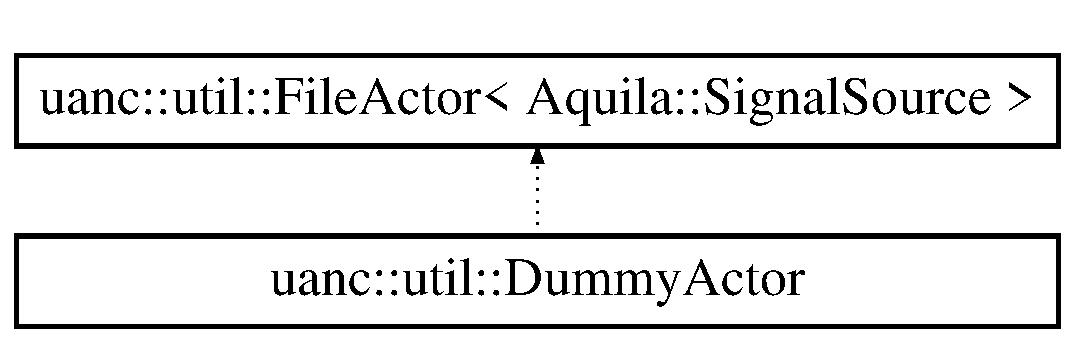
\includegraphics[height=2.000000cm]{classuanc_1_1util_1_1_dummy_actor}
\end{center}
\end{figure}
\subsection*{Public Member Functions}
\begin{DoxyCompactItemize}
\item 
\hyperlink{classuanc_1_1util_1_1_dummy_actor_abb98480739b7b401d41ccc68c8cba8a1}{Dummy\+Actor} (const std\+::string \&path)
\begin{DoxyCompactList}\small\item\em Basic constructor which saves a path string internally. \end{DoxyCompactList}\item 
std\+::shared\+\_\+ptr$<$ Aquila\+::\+Signal\+Source $>$ \hyperlink{classuanc_1_1util_1_1_dummy_actor_ae2912157674c282f5436f27ddbfcf8cc}{load\+Data} ()
\begin{DoxyCompactList}\small\item\em This method should load the file from the plate. \end{DoxyCompactList}\item 
void \hyperlink{classuanc_1_1util_1_1_dummy_actor_a321ba3ff6c3718d56edb6efe961f8230}{save\+Data} (std\+::shared\+\_\+ptr$<$ Aquila\+::\+Signal\+Source $>$ source)
\begin{DoxyCompactList}\small\item\em This method should save a file to the plate. \end{DoxyCompactList}\item 
\hyperlink{classuanc_1_1util_1_1_dummy_actor}{Dummy\+Actor} $\ast$ \hyperlink{classuanc_1_1util_1_1_dummy_actor_a5727b1ff300c340abd9216287592f9d9}{set\+Type} (std\+::string type)
\begin{DoxyCompactList}\small\item\em sets the type of the given string \end{DoxyCompactList}\item 
\hyperlink{classuanc_1_1util_1_1_dummy_actor}{Dummy\+Actor} $\ast$ \hyperlink{classuanc_1_1util_1_1_dummy_actor_a05d45731dce558047fff26bebd55e8ed}{set\+Frequency} (Aquila\+::\+Frequency\+Type frequency)
\begin{DoxyCompactList}\small\item\em sets the frequency \end{DoxyCompactList}\item 
\hyperlink{classuanc_1_1util_1_1_dummy_actor}{Dummy\+Actor} $\ast$ \hyperlink{classuanc_1_1util_1_1_dummy_actor_a3e14c7739566b336c5c60b187d033f24}{set\+Amplitude} (Aquila\+::\+Frequency\+Type amplitude)
\begin{DoxyCompactList}\small\item\em sets the amplitude of an Frequency\+Type \end{DoxyCompactList}\item 
\hyperlink{classuanc_1_1util_1_1_dummy_actor}{Dummy\+Actor} $\ast$ \hyperlink{classuanc_1_1util_1_1_dummy_actor_a9b52353146bb402cb422656a5d69983a}{set\+Sample\+Count} (size\+\_\+t count)
\begin{DoxyCompactList}\small\item\em sets the number of samples \end{DoxyCompactList}\end{DoxyCompactItemize}


\subsection{Constructor \& Destructor Documentation}
\index{uanc\+::util\+::\+Dummy\+Actor@{uanc\+::util\+::\+Dummy\+Actor}!Dummy\+Actor@{Dummy\+Actor}}
\index{Dummy\+Actor@{Dummy\+Actor}!uanc\+::util\+::\+Dummy\+Actor@{uanc\+::util\+::\+Dummy\+Actor}}
\subsubsection[{\texorpdfstring{Dummy\+Actor(const std\+::string \&path)}{DummyActor(const std::string &path)}}]{\setlength{\rightskip}{0pt plus 5cm}uanc\+::util\+::\+Dummy\+Actor\+::\+Dummy\+Actor (
\begin{DoxyParamCaption}
\item[{const std\+::string \&}]{path}
\end{DoxyParamCaption}
)\hspace{0.3cm}{\ttfamily [inline]}}\hypertarget{classuanc_1_1util_1_1_dummy_actor_abb98480739b7b401d41ccc68c8cba8a1}{}\label{classuanc_1_1util_1_1_dummy_actor_abb98480739b7b401d41ccc68c8cba8a1}


Basic constructor which saves a path string internally. 

This constructor just save the passed string internally.


\begin{DoxyParams}{Parameters}
{\em path} & The path to the acted file \\
\hline
\end{DoxyParams}


\subsection{Member Function Documentation}
\index{uanc\+::util\+::\+Dummy\+Actor@{uanc\+::util\+::\+Dummy\+Actor}!load\+Data@{load\+Data}}
\index{load\+Data@{load\+Data}!uanc\+::util\+::\+Dummy\+Actor@{uanc\+::util\+::\+Dummy\+Actor}}
\subsubsection[{\texorpdfstring{load\+Data()}{loadData()}}]{\setlength{\rightskip}{0pt plus 5cm}std\+::shared\+\_\+ptr$<$Aquila\+::\+Signal\+Source$>$ uanc\+::util\+::\+Dummy\+Actor\+::load\+Data (
\begin{DoxyParamCaption}
{}
\end{DoxyParamCaption}
)\hspace{0.3cm}{\ttfamily [inline]}, {\ttfamily [virtual]}}\hypertarget{classuanc_1_1util_1_1_dummy_actor_ae2912157674c282f5436f27ddbfcf8cc}{}\label{classuanc_1_1util_1_1_dummy_actor_ae2912157674c282f5436f27ddbfcf8cc}


This method should load the file from the plate. 

This method should return the loaded T

\begin{DoxyReturn}{Returns}
the loaded T 
\end{DoxyReturn}


Implements \hyperlink{classuanc_1_1util_1_1_file_actor_ad2db7584c9332a4d8376ccf6276ec301}{uanc\+::util\+::\+File\+Actor$<$ Aquila\+::\+Signal\+Source $>$}.

\index{uanc\+::util\+::\+Dummy\+Actor@{uanc\+::util\+::\+Dummy\+Actor}!save\+Data@{save\+Data}}
\index{save\+Data@{save\+Data}!uanc\+::util\+::\+Dummy\+Actor@{uanc\+::util\+::\+Dummy\+Actor}}
\subsubsection[{\texorpdfstring{save\+Data(std\+::shared\+\_\+ptr$<$ Aquila\+::\+Signal\+Source $>$ source)}{saveData(std::shared_ptr< Aquila::SignalSource > source)}}]{\setlength{\rightskip}{0pt plus 5cm}void uanc\+::util\+::\+Dummy\+Actor\+::save\+Data (
\begin{DoxyParamCaption}
\item[{std\+::shared\+\_\+ptr$<$ Aquila\+::\+Signal\+Source $>$}]{source}
\end{DoxyParamCaption}
)\hspace{0.3cm}{\ttfamily [inline]}, {\ttfamily [virtual]}}\hypertarget{classuanc_1_1util_1_1_dummy_actor_a321ba3ff6c3718d56edb6efe961f8230}{}\label{classuanc_1_1util_1_1_dummy_actor_a321ba3ff6c3718d56edb6efe961f8230}


This method should save a file to the plate. 

This should method should save the passed T to the specified path.


\begin{DoxyParams}{Parameters}
{\em source} & The source to save \\
\hline
\end{DoxyParams}


Implements \hyperlink{classuanc_1_1util_1_1_file_actor_aee5e36b37c46dda87f0499fc7b9e4b0d}{uanc\+::util\+::\+File\+Actor$<$ Aquila\+::\+Signal\+Source $>$}.

\index{uanc\+::util\+::\+Dummy\+Actor@{uanc\+::util\+::\+Dummy\+Actor}!set\+Amplitude@{set\+Amplitude}}
\index{set\+Amplitude@{set\+Amplitude}!uanc\+::util\+::\+Dummy\+Actor@{uanc\+::util\+::\+Dummy\+Actor}}
\subsubsection[{\texorpdfstring{set\+Amplitude(\+Aquila\+::\+Frequency\+Type amplitude)}{setAmplitude(Aquila::FrequencyType amplitude)}}]{\setlength{\rightskip}{0pt plus 5cm}{\bf Dummy\+Actor}$\ast$ uanc\+::util\+::\+Dummy\+Actor\+::set\+Amplitude (
\begin{DoxyParamCaption}
\item[{Aquila\+::\+Frequency\+Type}]{amplitude}
\end{DoxyParamCaption}
)\hspace{0.3cm}{\ttfamily [inline]}}\hypertarget{classuanc_1_1util_1_1_dummy_actor_a3e14c7739566b336c5c60b187d033f24}{}\label{classuanc_1_1util_1_1_dummy_actor_a3e14c7739566b336c5c60b187d033f24}


sets the amplitude of an Frequency\+Type 


\begin{DoxyParams}{Parameters}
{\em amplitude} & a Frequency\+Type \\
\hline
\end{DoxyParams}
\index{uanc\+::util\+::\+Dummy\+Actor@{uanc\+::util\+::\+Dummy\+Actor}!set\+Frequency@{set\+Frequency}}
\index{set\+Frequency@{set\+Frequency}!uanc\+::util\+::\+Dummy\+Actor@{uanc\+::util\+::\+Dummy\+Actor}}
\subsubsection[{\texorpdfstring{set\+Frequency(\+Aquila\+::\+Frequency\+Type frequency)}{setFrequency(Aquila::FrequencyType frequency)}}]{\setlength{\rightskip}{0pt plus 5cm}{\bf Dummy\+Actor}$\ast$ uanc\+::util\+::\+Dummy\+Actor\+::set\+Frequency (
\begin{DoxyParamCaption}
\item[{Aquila\+::\+Frequency\+Type}]{frequency}
\end{DoxyParamCaption}
)\hspace{0.3cm}{\ttfamily [inline]}}\hypertarget{classuanc_1_1util_1_1_dummy_actor_a05d45731dce558047fff26bebd55e8ed}{}\label{classuanc_1_1util_1_1_dummy_actor_a05d45731dce558047fff26bebd55e8ed}


sets the frequency 


\begin{DoxyParams}{Parameters}
{\em frequency} & a Frequency\+Type \\
\hline
\end{DoxyParams}
\index{uanc\+::util\+::\+Dummy\+Actor@{uanc\+::util\+::\+Dummy\+Actor}!set\+Sample\+Count@{set\+Sample\+Count}}
\index{set\+Sample\+Count@{set\+Sample\+Count}!uanc\+::util\+::\+Dummy\+Actor@{uanc\+::util\+::\+Dummy\+Actor}}
\subsubsection[{\texorpdfstring{set\+Sample\+Count(size\+\_\+t count)}{setSampleCount(size_t count)}}]{\setlength{\rightskip}{0pt plus 5cm}{\bf Dummy\+Actor}$\ast$ uanc\+::util\+::\+Dummy\+Actor\+::set\+Sample\+Count (
\begin{DoxyParamCaption}
\item[{size\+\_\+t}]{count}
\end{DoxyParamCaption}
)\hspace{0.3cm}{\ttfamily [inline]}}\hypertarget{classuanc_1_1util_1_1_dummy_actor_a9b52353146bb402cb422656a5d69983a}{}\label{classuanc_1_1util_1_1_dummy_actor_a9b52353146bb402cb422656a5d69983a}


sets the number of samples 


\begin{DoxyParams}{Parameters}
{\em count} & number of samples counted \\
\hline
\end{DoxyParams}
\index{uanc\+::util\+::\+Dummy\+Actor@{uanc\+::util\+::\+Dummy\+Actor}!set\+Type@{set\+Type}}
\index{set\+Type@{set\+Type}!uanc\+::util\+::\+Dummy\+Actor@{uanc\+::util\+::\+Dummy\+Actor}}
\subsubsection[{\texorpdfstring{set\+Type(std\+::string type)}{setType(std::string type)}}]{\setlength{\rightskip}{0pt plus 5cm}{\bf Dummy\+Actor}$\ast$ uanc\+::util\+::\+Dummy\+Actor\+::set\+Type (
\begin{DoxyParamCaption}
\item[{std\+::string}]{type}
\end{DoxyParamCaption}
)\hspace{0.3cm}{\ttfamily [inline]}}\hypertarget{classuanc_1_1util_1_1_dummy_actor_a5727b1ff300c340abd9216287592f9d9}{}\label{classuanc_1_1util_1_1_dummy_actor_a5727b1ff300c340abd9216287592f9d9}


sets the type of the given string 


\begin{DoxyParams}{Parameters}
{\em type} & string with the type \\
\hline
\end{DoxyParams}


The documentation for this class was generated from the following file\+:\begin{DoxyCompactItemize}
\item 
/home/kurt/\+Documents/\+Studium/\+Bachelor\+\_\+\+Praktikum/\+U\+A\+N\+C/\+Code/\+U\+A\+N\+C/util/\hyperlink{_dummy_actor_8h}{Dummy\+Actor.\+h}\end{DoxyCompactItemize}

\hypertarget{class_epsilon_tests}{}\section{Epsilon\+Tests Class Reference}
\label{class_epsilon_tests}\index{Epsilon\+Tests@{Epsilon\+Tests}}


{\ttfamily \#include $<$Epsilon\+Tests.\+h$>$}

\subsection*{Public Member Functions}
\begin{DoxyCompactItemize}
\item 
\hyperlink{class_epsilon_tests_ad99d3f7c8c7157ad89415a5a2e353444}{Epsilon\+Tests} ()
\begin{DoxyCompactList}\small\item\em This class can be used to check all algorithm. \end{DoxyCompactList}\item 
void \hyperlink{class_epsilon_tests_a55129393e25549a3129ef34df5660f81}{run} (std\+::string path)
\begin{DoxyCompactList}\small\item\em This methode runs all algorithm. \end{DoxyCompactList}\end{DoxyCompactItemize}


\subsection{Constructor \& Destructor Documentation}
\index{Epsilon\+Tests@{Epsilon\+Tests}!Epsilon\+Tests@{Epsilon\+Tests}}
\index{Epsilon\+Tests@{Epsilon\+Tests}!Epsilon\+Tests@{Epsilon\+Tests}}
\subsubsection[{\texorpdfstring{Epsilon\+Tests()}{EpsilonTests()}}]{\setlength{\rightskip}{0pt plus 5cm}Epsilon\+Tests\+::\+Epsilon\+Tests (
\begin{DoxyParamCaption}
{}
\end{DoxyParamCaption}
)}\hypertarget{class_epsilon_tests_ad99d3f7c8c7157ad89415a5a2e353444}{}\label{class_epsilon_tests_ad99d3f7c8c7157ad89415a5a2e353444}


This class can be used to check all algorithm. 

Gives a statistic for each algorithm. 

\subsection{Member Function Documentation}
\index{Epsilon\+Tests@{Epsilon\+Tests}!run@{run}}
\index{run@{run}!Epsilon\+Tests@{Epsilon\+Tests}}
\subsubsection[{\texorpdfstring{run(std\+::string path)}{run(std::string path)}}]{\setlength{\rightskip}{0pt plus 5cm}void Epsilon\+Tests\+::run (
\begin{DoxyParamCaption}
\item[{std\+::string}]{path}
\end{DoxyParamCaption}
)}\hypertarget{class_epsilon_tests_a55129393e25549a3129ef34df5660f81}{}\label{class_epsilon_tests_a55129393e25549a3129ef34df5660f81}


This methode runs all algorithm. 

Runs all algorithm and test if average error is smaler than epsilon 

The documentation for this class was generated from the following files\+:\begin{DoxyCompactItemize}
\item 
/ext/local/\+University/\+B\+P/\+Git/\+U\+A\+N\+C/\+Code/\+U\+A\+N\+C/util/tests/\hyperlink{_epsilon_tests_8h}{Epsilon\+Tests.\+h}\item 
/ext/local/\+University/\+B\+P/\+Git/\+U\+A\+N\+C/\+Code/\+U\+A\+N\+C/util/tests/\hyperlink{_epsilon_tests_8cpp}{Epsilon\+Tests.\+cpp}\end{DoxyCompactItemize}

\hypertarget{classuanc_1_1util_1_1event_1_1_event_container}{}\section{uanc\+:\+:util\+:\+:event\+:\+:Event\+Container Class Reference}
\label{classuanc_1_1util_1_1event_1_1_event_container}\index{uanc\+::util\+::event\+::\+Event\+Container@{uanc\+::util\+::event\+::\+Event\+Container}}


This is the event container.  




{\ttfamily \#include $<$Event\+Container.\+h$>$}

\subsection*{Public Member Functions}
\begin{DoxyCompactItemize}
\item 
void \hyperlink{classuanc_1_1util_1_1event_1_1_event_container_ac53f74b44d89a492b0ae55b585a0157d}{add} (std\+::string key, std\+::string value)
\begin{DoxyCompactList}\small\item\em Adds a key to the container. \end{DoxyCompactList}\item 
std\+::string \hyperlink{classuanc_1_1util_1_1event_1_1_event_container_a753a768f9df814994501cb398b8048c7}{get} (std\+::string key)
\begin{DoxyCompactList}\small\item\em Retrieves a key from the internal map. \end{DoxyCompactList}\end{DoxyCompactItemize}
\subsection*{Public Attributes}
\begin{DoxyCompactItemize}
\item 
int \hyperlink{classuanc_1_1util_1_1event_1_1_event_container_a27f819d0a217a8887c884cf2c69da4b7}{ID} = -\/1
\end{DoxyCompactItemize}


\subsection{Detailed Description}
This is the event container. 

This class describes the event container, in which your data gets wrapped when firing an event. 

\subsection{Member Function Documentation}
\index{uanc\+::util\+::event\+::\+Event\+Container@{uanc\+::util\+::event\+::\+Event\+Container}!add@{add}}
\index{add@{add}!uanc\+::util\+::event\+::\+Event\+Container@{uanc\+::util\+::event\+::\+Event\+Container}}
\subsubsection[{\texorpdfstring{add(std\+::string key, std\+::string value)}{add(std::string key, std::string value)}}]{\setlength{\rightskip}{0pt plus 5cm}void uanc\+::util\+::event\+::\+Event\+Container\+::add (
\begin{DoxyParamCaption}
\item[{std\+::string}]{key, }
\item[{std\+::string}]{value}
\end{DoxyParamCaption}
)\hspace{0.3cm}{\ttfamily [inline]}}\hypertarget{classuanc_1_1util_1_1event_1_1_event_container_ac53f74b44d89a492b0ae55b585a0157d}{}\label{classuanc_1_1util_1_1event_1_1_event_container_ac53f74b44d89a492b0ae55b585a0157d}


Adds a key to the container. 

This function takes a key and a value and adds it internally.


\begin{DoxyParams}{Parameters}
{\em key} & The key to add. \\
\hline
{\em value} & The value to add. \\
\hline
\end{DoxyParams}
\index{uanc\+::util\+::event\+::\+Event\+Container@{uanc\+::util\+::event\+::\+Event\+Container}!get@{get}}
\index{get@{get}!uanc\+::util\+::event\+::\+Event\+Container@{uanc\+::util\+::event\+::\+Event\+Container}}
\subsubsection[{\texorpdfstring{get(std\+::string key)}{get(std::string key)}}]{\setlength{\rightskip}{0pt plus 5cm}std\+::string uanc\+::util\+::event\+::\+Event\+Container\+::get (
\begin{DoxyParamCaption}
\item[{std\+::string}]{key}
\end{DoxyParamCaption}
)\hspace{0.3cm}{\ttfamily [inline]}}\hypertarget{classuanc_1_1util_1_1event_1_1_event_container_a753a768f9df814994501cb398b8048c7}{}\label{classuanc_1_1util_1_1event_1_1_event_container_a753a768f9df814994501cb398b8048c7}


Retrieves a key from the internal map. 


\begin{DoxyParams}{Parameters}
{\em key} & The key to retrieve. \\
\hline
\end{DoxyParams}
\begin{DoxyReturn}{Returns}
The value matching the key 
\end{DoxyReturn}


\subsection{Member Data Documentation}
\index{uanc\+::util\+::event\+::\+Event\+Container@{uanc\+::util\+::event\+::\+Event\+Container}!ID@{ID}}
\index{ID@{ID}!uanc\+::util\+::event\+::\+Event\+Container@{uanc\+::util\+::event\+::\+Event\+Container}}
\subsubsection[{\texorpdfstring{ID}{ID}}]{\setlength{\rightskip}{0pt plus 5cm}int uanc\+::util\+::event\+::\+Event\+Container\+::\+ID = -\/1}\hypertarget{classuanc_1_1util_1_1event_1_1_event_container_a27f819d0a217a8887c884cf2c69da4b7}{}\label{classuanc_1_1util_1_1event_1_1_event_container_a27f819d0a217a8887c884cf2c69da4b7}
Holds the id for the callee. 

The documentation for this class was generated from the following file\+:\begin{DoxyCompactItemize}
\item 
/home/kurt/\+Documents/\+Studium/\+Bachelor\+\_\+\+Praktikum/\+U\+A\+N\+C/\+Code/\+U\+A\+N\+C/util/event/\hyperlink{_event_container_8h}{Event\+Container.\+h}\end{DoxyCompactItemize}

\hypertarget{class_event_i_d_equal}{}\section{Event\+I\+D\+Equal Class Reference}
\label{class_event_i_d_equal}\index{Event\+I\+D\+Equal@{Event\+I\+D\+Equal}}


{\ttfamily \#include $<$Event\+Manager.\+h$>$}

\subsection*{Public Member Functions}
\begin{DoxyCompactItemize}
\item 
{\footnotesize template$<$typename T , typename U $>$ }\\bool \hyperlink{class_event_i_d_equal_a6d608a89305d63efacdf9c07df3502af}{operator()} (std\+::pair$<$ T, U $>$ const \&t1, std\+::pair$<$ T, U $>$ const \&t2) const 
\end{DoxyCompactItemize}


\subsection{Member Function Documentation}
\index{Event\+I\+D\+Equal@{Event\+I\+D\+Equal}!operator()@{operator()}}
\index{operator()@{operator()}!Event\+I\+D\+Equal@{Event\+I\+D\+Equal}}
\subsubsection[{\texorpdfstring{operator()(std\+::pair$<$ T, U $>$ const \&t1, std\+::pair$<$ T, U $>$ const \&t2) const }{operator()(std::pair< T, U > const &t1, std::pair< T, U > const &t2) const }}]{\setlength{\rightskip}{0pt plus 5cm}template$<$typename T , typename U $>$ bool Event\+I\+D\+Equal\+::operator() (
\begin{DoxyParamCaption}
\item[{std\+::pair$<$ T, U $>$ const \&}]{t1, }
\item[{std\+::pair$<$ T, U $>$ const \&}]{t2}
\end{DoxyParamCaption}
) const\hspace{0.3cm}{\ttfamily [inline]}}\hypertarget{class_event_i_d_equal_a6d608a89305d63efacdf9c07df3502af}{}\label{class_event_i_d_equal_a6d608a89305d63efacdf9c07df3502af}


The documentation for this class was generated from the following file\+:\begin{DoxyCompactItemize}
\item 
/home/kurt/\+Documents/\+Studium/\+Bachelor\+\_\+\+Praktikum/\+U\+A\+N\+C/\+Code/\+U\+A\+N\+C/util/event/\hyperlink{_event_manager_8h}{Event\+Manager.\+h}\end{DoxyCompactItemize}

\hypertarget{struct_event_i_d_hash}{}\section{Event\+I\+D\+Hash Struct Reference}
\label{struct_event_i_d_hash}\index{Event\+I\+D\+Hash@{Event\+I\+D\+Hash}}


{\ttfamily \#include $<$Event\+Manager.\+h$>$}

\subsection*{Public Member Functions}
\begin{DoxyCompactItemize}
\item 
{\footnotesize template$<$typename T , typename U $>$ }\\std\+::size\+\_\+t \hyperlink{struct_event_i_d_hash_ad85eec0b347d8e926c6ca4ad23582360}{operator()} (const std\+::pair$<$ T, U $>$ \&x) const 
\end{DoxyCompactItemize}


\subsection{Member Function Documentation}
\index{Event\+I\+D\+Hash@{Event\+I\+D\+Hash}!operator()@{operator()}}
\index{operator()@{operator()}!Event\+I\+D\+Hash@{Event\+I\+D\+Hash}}
\subsubsection[{\texorpdfstring{operator()(const std\+::pair$<$ T, U $>$ \&x) const }{operator()(const std::pair< T, U > &x) const }}]{\setlength{\rightskip}{0pt plus 5cm}template$<$typename T , typename U $>$ std\+::size\+\_\+t Event\+I\+D\+Hash\+::operator() (
\begin{DoxyParamCaption}
\item[{const std\+::pair$<$ T, U $>$ \&}]{x}
\end{DoxyParamCaption}
) const\hspace{0.3cm}{\ttfamily [inline]}}\hypertarget{struct_event_i_d_hash_ad85eec0b347d8e926c6ca4ad23582360}{}\label{struct_event_i_d_hash_ad85eec0b347d8e926c6ca4ad23582360}


The documentation for this struct was generated from the following file\+:\begin{DoxyCompactItemize}
\item 
/ext/local/\+University/\+B\+P/\+Git/\+U\+A\+N\+C/\+Code/\+U\+A\+N\+C/util/event/\hyperlink{_event_manager_8h}{Event\+Manager.\+h}\end{DoxyCompactItemize}

\hypertarget{classuanc_1_1util_1_1event_1_1_event_manager}{}\section{uanc\+:\+:util\+:\+:event\+:\+:Event\+Manager Class Reference}
\label{classuanc_1_1util_1_1event_1_1_event_manager}\index{uanc\+::util\+::event\+::\+Event\+Manager@{uanc\+::util\+::event\+::\+Event\+Manager}}


Simple event manager.  




{\ttfamily \#include $<$Event\+Manager.\+h$>$}

\subsection*{Public Member Functions}
\begin{DoxyCompactItemize}
\item 
\hyperlink{classuanc_1_1util_1_1event_1_1_event_manager_a333c19840c05d0785631b1bfc6bf6454}{$\sim$\+Event\+Manager} ()
\begin{DoxyCompactList}\small\item\em Basic destructor. \end{DoxyCompactList}\end{DoxyCompactItemize}
\subsection*{Static Public Member Functions}
\begin{DoxyCompactItemize}
\item 
static void \hyperlink{classuanc_1_1util_1_1event_1_1_event_manager_a344b7c080fb7d569c2b4948cbe8fbb7e}{destroy} ()
\end{DoxyCompactItemize}
\subsection*{Friends}
\begin{DoxyCompactItemize}
\item 
class \hyperlink{classuanc_1_1util_1_1event_1_1_event_manager_ac94178afc9fbbac2a5735d761b6b2ae5}{Event\+Token}
\item 
class \hyperlink{classuanc_1_1util_1_1event_1_1_event_manager_a7512992e19dc2f4613dea5e056e626f9}{Event\+Observer}
\end{DoxyCompactItemize}


\subsection{Detailed Description}
Simple event manager. 

This class represents the event manager and can be accessed via the singleton pattern from all classes which are friends of this one. 

\subsection{Constructor \& Destructor Documentation}
\index{uanc\+::util\+::event\+::\+Event\+Manager@{uanc\+::util\+::event\+::\+Event\+Manager}!````~Event\+Manager@{$\sim$\+Event\+Manager}}
\index{````~Event\+Manager@{$\sim$\+Event\+Manager}!uanc\+::util\+::event\+::\+Event\+Manager@{uanc\+::util\+::event\+::\+Event\+Manager}}
\subsubsection[{\texorpdfstring{$\sim$\+Event\+Manager()}{~EventManager()}}]{\setlength{\rightskip}{0pt plus 5cm}uanc\+::util\+::event\+::\+Event\+Manager\+::$\sim$\+Event\+Manager (
\begin{DoxyParamCaption}
{}
\end{DoxyParamCaption}
)}\hypertarget{classuanc_1_1util_1_1event_1_1_event_manager_a333c19840c05d0785631b1bfc6bf6454}{}\label{classuanc_1_1util_1_1event_1_1_event_manager_a333c19840c05d0785631b1bfc6bf6454}


Basic destructor. 

This deconstructore destroys the registered instance. 

\subsection{Member Function Documentation}
\index{uanc\+::util\+::event\+::\+Event\+Manager@{uanc\+::util\+::event\+::\+Event\+Manager}!destroy@{destroy}}
\index{destroy@{destroy}!uanc\+::util\+::event\+::\+Event\+Manager@{uanc\+::util\+::event\+::\+Event\+Manager}}
\subsubsection[{\texorpdfstring{destroy()}{destroy()}}]{\setlength{\rightskip}{0pt plus 5cm}void uanc\+::util\+::event\+::\+Event\+Manager\+::destroy (
\begin{DoxyParamCaption}
{}
\end{DoxyParamCaption}
)\hspace{0.3cm}{\ttfamily [static]}}\hypertarget{classuanc_1_1util_1_1event_1_1_event_manager_a344b7c080fb7d569c2b4948cbe8fbb7e}{}\label{classuanc_1_1util_1_1event_1_1_event_manager_a344b7c080fb7d569c2b4948cbe8fbb7e}
This method gets called to destroy the event manager. 

\subsection{Friends And Related Function Documentation}
\index{uanc\+::util\+::event\+::\+Event\+Manager@{uanc\+::util\+::event\+::\+Event\+Manager}!Event\+Observer@{Event\+Observer}}
\index{Event\+Observer@{Event\+Observer}!uanc\+::util\+::event\+::\+Event\+Manager@{uanc\+::util\+::event\+::\+Event\+Manager}}
\subsubsection[{\texorpdfstring{Event\+Observer}{EventObserver}}]{\setlength{\rightskip}{0pt plus 5cm}friend class {\bf Event\+Observer}\hspace{0.3cm}{\ttfamily [friend]}}\hypertarget{classuanc_1_1util_1_1event_1_1_event_manager_a7512992e19dc2f4613dea5e056e626f9}{}\label{classuanc_1_1util_1_1event_1_1_event_manager_a7512992e19dc2f4613dea5e056e626f9}
\index{uanc\+::util\+::event\+::\+Event\+Manager@{uanc\+::util\+::event\+::\+Event\+Manager}!Event\+Token@{Event\+Token}}
\index{Event\+Token@{Event\+Token}!uanc\+::util\+::event\+::\+Event\+Manager@{uanc\+::util\+::event\+::\+Event\+Manager}}
\subsubsection[{\texorpdfstring{Event\+Token}{EventToken}}]{\setlength{\rightskip}{0pt plus 5cm}friend class {\bf Event\+Token}\hspace{0.3cm}{\ttfamily [friend]}}\hypertarget{classuanc_1_1util_1_1event_1_1_event_manager_ac94178afc9fbbac2a5735d761b6b2ae5}{}\label{classuanc_1_1util_1_1event_1_1_event_manager_ac94178afc9fbbac2a5735d761b6b2ae5}


The documentation for this class was generated from the following files\+:\begin{DoxyCompactItemize}
\item 
/ext/local/\+University/\+B\+P/\+Git/\+U\+A\+N\+C/\+Code/\+U\+A\+N\+C/util/event/\hyperlink{_event_manager_8h}{Event\+Manager.\+h}\item 
/ext/local/\+University/\+B\+P/\+Git/\+U\+A\+N\+C/\+Code/\+U\+A\+N\+C/util/event/\hyperlink{_event_manager_8cpp}{Event\+Manager.\+cpp}\end{DoxyCompactItemize}

\hypertarget{classuanc_1_1util_1_1event_1_1_event_observer}{}\section{uanc\+:\+:util\+:\+:event\+:\+:Event\+Observer Class Reference}
\label{classuanc_1_1util_1_1event_1_1_event_observer}\index{uanc\+::util\+::event\+::\+Event\+Observer@{uanc\+::util\+::event\+::\+Event\+Observer}}


Represents the observer interface.  




{\ttfamily \#include $<$Event\+Observer.\+h$>$}

Inheritance diagram for uanc\+:\+:util\+:\+:event\+:\+:Event\+Observer\+:\begin{figure}[H]
\begin{center}
\leavevmode
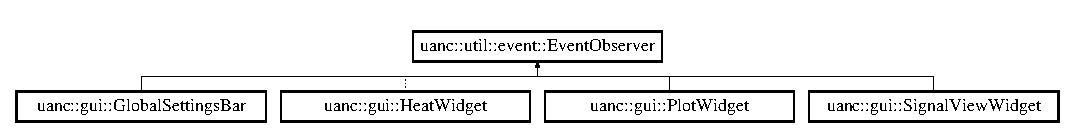
\includegraphics[height=1.407035cm]{classuanc_1_1util_1_1event_1_1_event_observer}
\end{center}
\end{figure}
\subsection*{Protected Member Functions}
\begin{DoxyCompactItemize}
\item 
\hyperlink{classuanc_1_1util_1_1event_1_1_event_observer_a0b2188938471e358af093489db73c490}{Event\+Observer} (std\+::initializer\+\_\+list$<$ \hyperlink{namespaceuanc_1_1util_1_1event_a63f690675589114db9c6bcbe6f1088a4}{Events} $>$ events)
\begin{DoxyCompactList}\small\item\em Constructor for observing the event. \end{DoxyCompactList}\item 
\hyperlink{classuanc_1_1util_1_1event_1_1_event_observer_a026ac27f3295ed3d56b3f4d34af8c0bb}{$\sim$\+Event\+Observer} ()
\begin{DoxyCompactList}\small\item\em Deconstructor. \end{DoxyCompactList}\item 
virtual void \hyperlink{classuanc_1_1util_1_1event_1_1_event_observer_af1640e34db3379eaba8c817a92199807}{triggered} (\hyperlink{namespaceuanc_1_1util_1_1event_a63f690675589114db9c6bcbe6f1088a4}{Events} event, \hyperlink{classuanc_1_1util_1_1event_1_1_event_container}{Event\+Container} data)=0
\begin{DoxyCompactList}\small\item\em Override to catch event. \end{DoxyCompactList}\end{DoxyCompactItemize}
\subsection*{Protected Attributes}
\begin{DoxyCompactItemize}
\item 
\hyperlink{classuanc_1_1util_1_1event_1_1_event_token}{Event\+Token} $\ast$ \hyperlink{classuanc_1_1util_1_1event_1_1_event_observer_a71e5e39d89518e1ec0018227ddd3c368}{\+\_\+token}
\begin{DoxyCompactList}\small\item\em Unique Pointer to the token. \end{DoxyCompactList}\end{DoxyCompactItemize}
\subsection*{Friends}
\begin{DoxyCompactItemize}
\item 
class \hyperlink{classuanc_1_1util_1_1event_1_1_event_observer_aba45a46c615e2683daffdae82e2d3b8f}{Event\+Manager}
\end{DoxyCompactItemize}


\subsection{Detailed Description}
Represents the observer interface. 

This class is an event observer. Simply derive from it to let a class access the event system. 

\subsection{Constructor \& Destructor Documentation}
\index{uanc\+::util\+::event\+::\+Event\+Observer@{uanc\+::util\+::event\+::\+Event\+Observer}!Event\+Observer@{Event\+Observer}}
\index{Event\+Observer@{Event\+Observer}!uanc\+::util\+::event\+::\+Event\+Observer@{uanc\+::util\+::event\+::\+Event\+Observer}}
\subsubsection[{\texorpdfstring{Event\+Observer(std\+::initializer\+\_\+list$<$ Events $>$ events)}{EventObserver(std::initializer_list< Events > events)}}]{\setlength{\rightskip}{0pt plus 5cm}uanc\+::util\+::event\+::\+Event\+Observer\+::\+Event\+Observer (
\begin{DoxyParamCaption}
\item[{std\+::initializer\+\_\+list$<$ {\bf Events} $>$}]{events}
\end{DoxyParamCaption}
)\hspace{0.3cm}{\ttfamily [protected]}}\hypertarget{classuanc_1_1util_1_1event_1_1_event_observer_a0b2188938471e358af093489db73c490}{}\label{classuanc_1_1util_1_1event_1_1_event_observer_a0b2188938471e358af093489db73c490}


Constructor for observing the event. 

This constructor can be used register all neccessary events inside.


\begin{DoxyParams}{Parameters}
{\em events} & The events to register. \\
\hline
\end{DoxyParams}
\index{uanc\+::util\+::event\+::\+Event\+Observer@{uanc\+::util\+::event\+::\+Event\+Observer}!````~Event\+Observer@{$\sim$\+Event\+Observer}}
\index{````~Event\+Observer@{$\sim$\+Event\+Observer}!uanc\+::util\+::event\+::\+Event\+Observer@{uanc\+::util\+::event\+::\+Event\+Observer}}
\subsubsection[{\texorpdfstring{$\sim$\+Event\+Observer()}{~EventObserver()}}]{\setlength{\rightskip}{0pt plus 5cm}uanc\+::util\+::event\+::\+Event\+Observer\+::$\sim$\+Event\+Observer (
\begin{DoxyParamCaption}
{}
\end{DoxyParamCaption}
)\hspace{0.3cm}{\ttfamily [protected]}}\hypertarget{classuanc_1_1util_1_1event_1_1_event_observer_a026ac27f3295ed3d56b3f4d34af8c0bb}{}\label{classuanc_1_1util_1_1event_1_1_event_observer_a026ac27f3295ed3d56b3f4d34af8c0bb}


Deconstructor. 

This deconstructor can be used to deregister the token. 

\subsection{Member Function Documentation}
\index{uanc\+::util\+::event\+::\+Event\+Observer@{uanc\+::util\+::event\+::\+Event\+Observer}!triggered@{triggered}}
\index{triggered@{triggered}!uanc\+::util\+::event\+::\+Event\+Observer@{uanc\+::util\+::event\+::\+Event\+Observer}}
\subsubsection[{\texorpdfstring{triggered(\+Events event, Event\+Container data)=0}{triggered(Events event, EventContainer data)=0}}]{\setlength{\rightskip}{0pt plus 5cm}virtual void uanc\+::util\+::event\+::\+Event\+Observer\+::triggered (
\begin{DoxyParamCaption}
\item[{{\bf Events}}]{event, }
\item[{{\bf Event\+Container}}]{data}
\end{DoxyParamCaption}
)\hspace{0.3cm}{\ttfamily [protected]}, {\ttfamily [pure virtual]}}\hypertarget{classuanc_1_1util_1_1event_1_1_event_observer_af1640e34db3379eaba8c817a92199807}{}\label{classuanc_1_1util_1_1event_1_1_event_observer_af1640e34db3379eaba8c817a92199807}


Override to catch event. 

This can be used, to integrate a handling to a specific event.


\begin{DoxyParams}{Parameters}
{\em event} & The event which should be triggered. \\
\hline
{\em data} & The data to supply. \\
\hline
\end{DoxyParams}


Implemented in \hyperlink{classuanc_1_1gui_1_1_heat_widget_afe92e65ebf7d607ef7e1d40aaaa6131a}{uanc\+::gui\+::\+Heat\+Widget}, \hyperlink{classuanc_1_1gui_1_1_global_settings_bar_a780fabb890235753ff90c1403638c47d}{uanc\+::gui\+::\+Global\+Settings\+Bar}, and \hyperlink{classuanc_1_1gui_1_1_signal_view_widget_a2f070824372de0e83960814229d93b46}{uanc\+::gui\+::\+Signal\+View\+Widget}.



\subsection{Friends And Related Function Documentation}
\index{uanc\+::util\+::event\+::\+Event\+Observer@{uanc\+::util\+::event\+::\+Event\+Observer}!Event\+Manager@{Event\+Manager}}
\index{Event\+Manager@{Event\+Manager}!uanc\+::util\+::event\+::\+Event\+Observer@{uanc\+::util\+::event\+::\+Event\+Observer}}
\subsubsection[{\texorpdfstring{Event\+Manager}{EventManager}}]{\setlength{\rightskip}{0pt plus 5cm}friend class {\bf Event\+Manager}\hspace{0.3cm}{\ttfamily [friend]}}\hypertarget{classuanc_1_1util_1_1event_1_1_event_observer_aba45a46c615e2683daffdae82e2d3b8f}{}\label{classuanc_1_1util_1_1event_1_1_event_observer_aba45a46c615e2683daffdae82e2d3b8f}


\subsection{Member Data Documentation}
\index{uanc\+::util\+::event\+::\+Event\+Observer@{uanc\+::util\+::event\+::\+Event\+Observer}!\+\_\+token@{\+\_\+token}}
\index{\+\_\+token@{\+\_\+token}!uanc\+::util\+::event\+::\+Event\+Observer@{uanc\+::util\+::event\+::\+Event\+Observer}}
\subsubsection[{\texorpdfstring{\+\_\+token}{_token}}]{\setlength{\rightskip}{0pt plus 5cm}{\bf Event\+Token}$\ast$ uanc\+::util\+::event\+::\+Event\+Observer\+::\+\_\+token\hspace{0.3cm}{\ttfamily [protected]}}\hypertarget{classuanc_1_1util_1_1event_1_1_event_observer_a71e5e39d89518e1ec0018227ddd3c368}{}\label{classuanc_1_1util_1_1event_1_1_event_observer_a71e5e39d89518e1ec0018227ddd3c368}


Unique Pointer to the token. 

This can be used to access the token. 

The documentation for this class was generated from the following files\+:\begin{DoxyCompactItemize}
\item 
/home/kurt/\+Documents/\+Studium/\+Bachelor\+\_\+\+Praktikum/\+U\+A\+N\+C/\+Code/\+U\+A\+N\+C/util/event/\hyperlink{_event_observer_8h}{Event\+Observer.\+h}\item 
/home/kurt/\+Documents/\+Studium/\+Bachelor\+\_\+\+Praktikum/\+U\+A\+N\+C/\+Code/\+U\+A\+N\+C/util/event/\hyperlink{_event_observer_8cpp}{Event\+Observer.\+cpp}\end{DoxyCompactItemize}

\hypertarget{classuanc_1_1util_1_1event_1_1_event_token}{}\section{uanc\+:\+:util\+:\+:event\+:\+:Event\+Token Class Reference}
\label{classuanc_1_1util_1_1event_1_1_event_token}\index{uanc\+::util\+::event\+::\+Event\+Token@{uanc\+::util\+::event\+::\+Event\+Token}}


Token retrieved by the eventsystem.  




{\ttfamily \#include $<$Event\+Token.\+h$>$}

\subsection*{Public Member Functions}
\begin{DoxyCompactItemize}
\item 
void \hyperlink{classuanc_1_1util_1_1event_1_1_event_token_a2bd43e6e227119b4b55a1a3adc7dd22c}{trigger} (\hyperlink{namespaceuanc_1_1util_1_1event_a63f690675589114db9c6bcbe6f1088a4}{Events} event, \hyperlink{classuanc_1_1util_1_1event_1_1_event_container}{Event\+Container} data)
\begin{DoxyCompactList}\small\item\em Call this method to trigger an event. \end{DoxyCompactList}\item 
\hyperlink{classuanc_1_1util_1_1event_1_1_event_container}{Event\+Container} \hyperlink{classuanc_1_1util_1_1event_1_1_event_token_ab2996160dd25090ef19681dcac70e302}{get\+Last\+Event} (\hyperlink{namespaceuanc_1_1util_1_1event_a63f690675589114db9c6bcbe6f1088a4}{Events} event)
\item 
bool \hyperlink{classuanc_1_1util_1_1event_1_1_event_token_ad0ee869b12bf8dfc3d7daa2aeb10d71f}{has\+Last\+Event} (\hyperlink{namespaceuanc_1_1util_1_1event_a63f690675589114db9c6bcbe6f1088a4}{Events} event)
\item 
void \hyperlink{classuanc_1_1util_1_1event_1_1_event_token_a8e7086a70365a2cd3d5e759fdae20b30}{delete\+Last\+Event} (\hyperlink{namespaceuanc_1_1util_1_1event_a63f690675589114db9c6bcbe6f1088a4}{Events} event)
\end{DoxyCompactItemize}
\subsection*{Friends}
\begin{DoxyCompactItemize}
\item 
class \hyperlink{classuanc_1_1util_1_1event_1_1_event_token_aba45a46c615e2683daffdae82e2d3b8f}{Event\+Manager}
\item 
class \hyperlink{classuanc_1_1util_1_1event_1_1_event_token_a7512992e19dc2f4613dea5e056e626f9}{Event\+Observer}
\end{DoxyCompactItemize}


\subsection{Detailed Description}
Token retrieved by the eventsystem. 

This token describes the access of a class to the eventsystem. Every instance will be handled as a unqiue one. 

\subsection{Member Function Documentation}
\index{uanc\+::util\+::event\+::\+Event\+Token@{uanc\+::util\+::event\+::\+Event\+Token}!delete\+Last\+Event@{delete\+Last\+Event}}
\index{delete\+Last\+Event@{delete\+Last\+Event}!uanc\+::util\+::event\+::\+Event\+Token@{uanc\+::util\+::event\+::\+Event\+Token}}
\subsubsection[{\texorpdfstring{delete\+Last\+Event(\+Events event)}{deleteLastEvent(Events event)}}]{\setlength{\rightskip}{0pt plus 5cm}void uanc\+::util\+::event\+::\+Event\+Token\+::delete\+Last\+Event (
\begin{DoxyParamCaption}
\item[{{\bf Events}}]{event}
\end{DoxyParamCaption}
)}\hypertarget{classuanc_1_1util_1_1event_1_1_event_token_a8e7086a70365a2cd3d5e759fdae20b30}{}\label{classuanc_1_1util_1_1event_1_1_event_token_a8e7086a70365a2cd3d5e759fdae20b30}
Can be used to delete the last event. \index{uanc\+::util\+::event\+::\+Event\+Token@{uanc\+::util\+::event\+::\+Event\+Token}!get\+Last\+Event@{get\+Last\+Event}}
\index{get\+Last\+Event@{get\+Last\+Event}!uanc\+::util\+::event\+::\+Event\+Token@{uanc\+::util\+::event\+::\+Event\+Token}}
\subsubsection[{\texorpdfstring{get\+Last\+Event(\+Events event)}{getLastEvent(Events event)}}]{\setlength{\rightskip}{0pt plus 5cm}{\bf Event\+Container} uanc\+::util\+::event\+::\+Event\+Token\+::get\+Last\+Event (
\begin{DoxyParamCaption}
\item[{{\bf Events}}]{event}
\end{DoxyParamCaption}
)}\hypertarget{classuanc_1_1util_1_1event_1_1_event_token_ab2996160dd25090ef19681dcac70e302}{}\label{classuanc_1_1util_1_1event_1_1_event_token_ab2996160dd25090ef19681dcac70e302}
Can be used to get the last event \index{uanc\+::util\+::event\+::\+Event\+Token@{uanc\+::util\+::event\+::\+Event\+Token}!has\+Last\+Event@{has\+Last\+Event}}
\index{has\+Last\+Event@{has\+Last\+Event}!uanc\+::util\+::event\+::\+Event\+Token@{uanc\+::util\+::event\+::\+Event\+Token}}
\subsubsection[{\texorpdfstring{has\+Last\+Event(\+Events event)}{hasLastEvent(Events event)}}]{\setlength{\rightskip}{0pt plus 5cm}bool uanc\+::util\+::event\+::\+Event\+Token\+::has\+Last\+Event (
\begin{DoxyParamCaption}
\item[{{\bf Events}}]{event}
\end{DoxyParamCaption}
)}\hypertarget{classuanc_1_1util_1_1event_1_1_event_token_ad0ee869b12bf8dfc3d7daa2aeb10d71f}{}\label{classuanc_1_1util_1_1event_1_1_event_token_ad0ee869b12bf8dfc3d7daa2aeb10d71f}
Can be used to get the last event \index{uanc\+::util\+::event\+::\+Event\+Token@{uanc\+::util\+::event\+::\+Event\+Token}!trigger@{trigger}}
\index{trigger@{trigger}!uanc\+::util\+::event\+::\+Event\+Token@{uanc\+::util\+::event\+::\+Event\+Token}}
\subsubsection[{\texorpdfstring{trigger(\+Events event, Event\+Container data)}{trigger(Events event, EventContainer data)}}]{\setlength{\rightskip}{0pt plus 5cm}void uanc\+::util\+::event\+::\+Event\+Token\+::trigger (
\begin{DoxyParamCaption}
\item[{{\bf Events}}]{event, }
\item[{{\bf Event\+Container}}]{data}
\end{DoxyParamCaption}
)}\hypertarget{classuanc_1_1util_1_1event_1_1_event_token_a2bd43e6e227119b4b55a1a3adc7dd22c}{}\label{classuanc_1_1util_1_1event_1_1_event_token_a2bd43e6e227119b4b55a1a3adc7dd22c}


Call this method to trigger an event. 

This can be called to trigger an event. Therefore you need to supply an event and a data container.


\begin{DoxyParams}{Parameters}
{\em event} & The event to trigger. \\
\hline
{\em data} & The data to pass with the event. \\
\hline
\end{DoxyParams}


\subsection{Friends And Related Function Documentation}
\index{uanc\+::util\+::event\+::\+Event\+Token@{uanc\+::util\+::event\+::\+Event\+Token}!Event\+Manager@{Event\+Manager}}
\index{Event\+Manager@{Event\+Manager}!uanc\+::util\+::event\+::\+Event\+Token@{uanc\+::util\+::event\+::\+Event\+Token}}
\subsubsection[{\texorpdfstring{Event\+Manager}{EventManager}}]{\setlength{\rightskip}{0pt plus 5cm}friend class {\bf Event\+Manager}\hspace{0.3cm}{\ttfamily [friend]}}\hypertarget{classuanc_1_1util_1_1event_1_1_event_token_aba45a46c615e2683daffdae82e2d3b8f}{}\label{classuanc_1_1util_1_1event_1_1_event_token_aba45a46c615e2683daffdae82e2d3b8f}
\index{uanc\+::util\+::event\+::\+Event\+Token@{uanc\+::util\+::event\+::\+Event\+Token}!Event\+Observer@{Event\+Observer}}
\index{Event\+Observer@{Event\+Observer}!uanc\+::util\+::event\+::\+Event\+Token@{uanc\+::util\+::event\+::\+Event\+Token}}
\subsubsection[{\texorpdfstring{Event\+Observer}{EventObserver}}]{\setlength{\rightskip}{0pt plus 5cm}friend class {\bf Event\+Observer}\hspace{0.3cm}{\ttfamily [friend]}}\hypertarget{classuanc_1_1util_1_1event_1_1_event_token_a7512992e19dc2f4613dea5e056e626f9}{}\label{classuanc_1_1util_1_1event_1_1_event_token_a7512992e19dc2f4613dea5e056e626f9}


The documentation for this class was generated from the following files\+:\begin{DoxyCompactItemize}
\item 
/ext/local/\+University/\+B\+P/\+Git/\+U\+A\+N\+C/\+Code/\+U\+A\+N\+C/util/event/\hyperlink{_event_token_8h}{Event\+Token.\+h}\item 
/ext/local/\+University/\+B\+P/\+Git/\+U\+A\+N\+C/\+Code/\+U\+A\+N\+C/util/event/\hyperlink{_event_token_8cpp}{Event\+Token.\+cpp}\end{DoxyCompactItemize}

\hypertarget{classuanc_1_1amv_1_1signal_1_1model_1_1_f_f_t_model}{}\section{uanc\+:\+:amv\+:\+:signal\+:\+:model\+:\+:F\+F\+T\+Model Class Reference}
\label{classuanc_1_1amv_1_1signal_1_1model_1_1_f_f_t_model}\index{uanc\+::amv\+::signal\+::model\+::\+F\+F\+T\+Model@{uanc\+::amv\+::signal\+::model\+::\+F\+F\+T\+Model}}


This is a model for the transformation of a signal to a spectrogram representation.  




{\ttfamily \#include $<$F\+F\+T\+Model.\+h$>$}

Inheritance diagram for uanc\+:\+:amv\+:\+:signal\+:\+:model\+:\+:F\+F\+T\+Model\+:\begin{figure}[H]
\begin{center}
\leavevmode
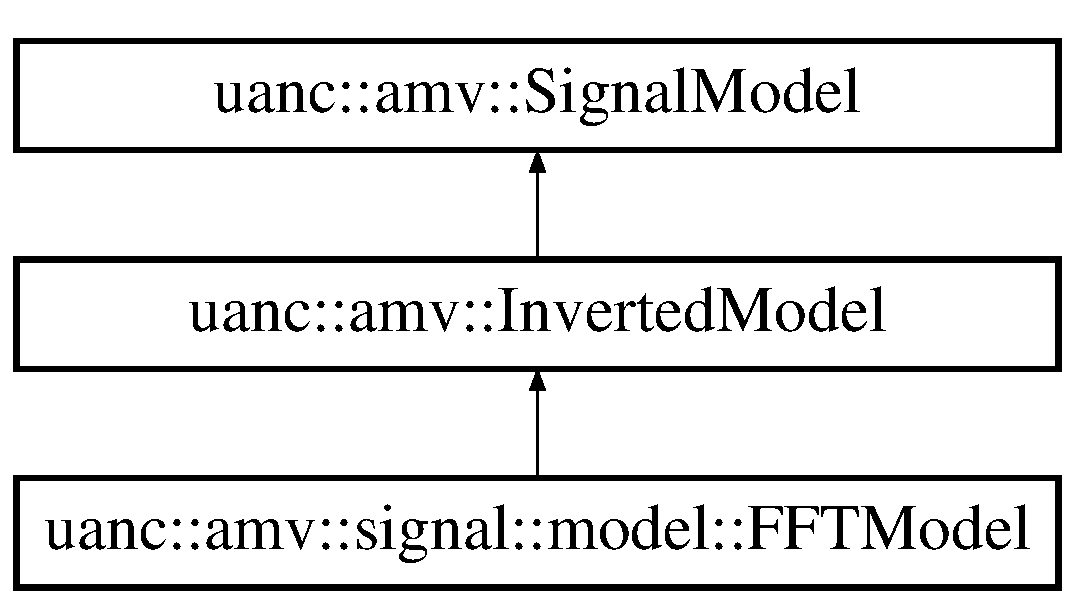
\includegraphics[height=3.000000cm]{classuanc_1_1amv_1_1signal_1_1model_1_1_f_f_t_model}
\end{center}
\end{figure}
\subsection*{Public Attributes}
\begin{DoxyCompactItemize}
\item 
std\+::shared\+\_\+ptr$<$ \hyperlink{classuanc_1_1amv_1_1_inverted_model}{uanc\+::amv\+::\+Inverted\+Model} $>$ \hyperlink{classuanc_1_1amv_1_1signal_1_1model_1_1_f_f_t_model_a1a63228d3c06b13ffb95038823fac3ae}{fft\+Signal}
\begin{DoxyCompactList}\small\item\em Holds the spectrum. \end{DoxyCompactList}\end{DoxyCompactItemize}


\subsection{Detailed Description}
This is a model for the transformation of a signal to a spectrogram representation. 

It used by the Fourier\+Transformation\+Algorithm. 

\subsection{Member Data Documentation}
\index{uanc\+::amv\+::signal\+::model\+::\+F\+F\+T\+Model@{uanc\+::amv\+::signal\+::model\+::\+F\+F\+T\+Model}!fft\+Signal@{fft\+Signal}}
\index{fft\+Signal@{fft\+Signal}!uanc\+::amv\+::signal\+::model\+::\+F\+F\+T\+Model@{uanc\+::amv\+::signal\+::model\+::\+F\+F\+T\+Model}}
\subsubsection[{\texorpdfstring{fft\+Signal}{fftSignal}}]{\setlength{\rightskip}{0pt plus 5cm}std\+::shared\+\_\+ptr$<${\bf uanc\+::amv\+::\+Inverted\+Model}$>$ uanc\+::amv\+::signal\+::model\+::\+F\+F\+T\+Model\+::fft\+Signal}\hypertarget{classuanc_1_1amv_1_1signal_1_1model_1_1_f_f_t_model_a1a63228d3c06b13ffb95038823fac3ae}{}\label{classuanc_1_1amv_1_1signal_1_1model_1_1_f_f_t_model_a1a63228d3c06b13ffb95038823fac3ae}


Holds the spectrum. 

This field holds the spectrum of the original signal. 

The documentation for this class was generated from the following file\+:\begin{DoxyCompactItemize}
\item 
/ext/local/\+University/\+B\+P/\+Git/\+U\+A\+N\+C/\+Code/\+U\+A\+N\+C/amv/signal/model/\hyperlink{_f_f_t_model_8h}{F\+F\+T\+Model.\+h}\end{DoxyCompactItemize}

\hypertarget{classuanc_1_1amv_1_1signal_1_1algorithm_1_1_f_f_t_transformation_algorithm}{}\section{uanc\+:\+:amv\+:\+:signal\+:\+:algorithm\+:\+:F\+F\+T\+Transformation\+Algorithm Class Reference}
\label{classuanc_1_1amv_1_1signal_1_1algorithm_1_1_f_f_t_transformation_algorithm}\index{uanc\+::amv\+::signal\+::algorithm\+::\+F\+F\+T\+Transformation\+Algorithm@{uanc\+::amv\+::signal\+::algorithm\+::\+F\+F\+T\+Transformation\+Algorithm}}


Transforms the view of a signal into Fourier space using F\+FT.  




{\ttfamily \#include $<$F\+F\+T\+Transformation\+Algorithm.\+h$>$}

Inheritance diagram for uanc\+:\+:amv\+:\+:signal\+:\+:algorithm\+:\+:F\+F\+T\+Transformation\+Algorithm\+:\begin{figure}[H]
\begin{center}
\leavevmode
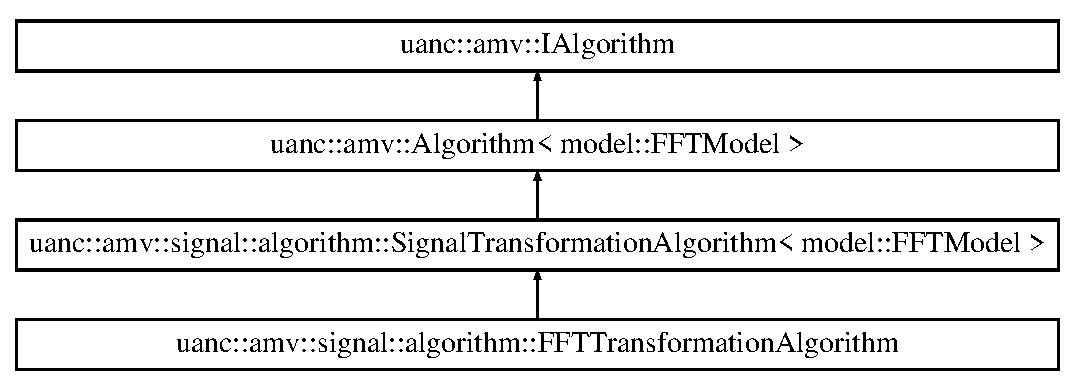
\includegraphics[height=4.000000cm]{classuanc_1_1amv_1_1signal_1_1algorithm_1_1_f_f_t_transformation_algorithm}
\end{center}
\end{figure}
\subsection*{Public Member Functions}
\begin{DoxyCompactItemize}
\item 
std\+::string \hyperlink{classuanc_1_1amv_1_1signal_1_1algorithm_1_1_f_f_t_transformation_algorithm_a07338debb7f34446fba77b6982174727}{get\+Name} () final
\begin{DoxyCompactList}\small\item\em Returns the name of the transformed data representation. \end{DoxyCompactList}\item 
void \hyperlink{classuanc_1_1amv_1_1signal_1_1algorithm_1_1_f_f_t_transformation_algorithm_a0748e30e870a462a10220cb07c784f2a}{transform} (std\+::shared\+\_\+ptr$<$ \hyperlink{classuanc_1_1amv_1_1_inverted_model}{uanc\+::amv\+::\+Inverted\+Model} $>$ in) final
\begin{DoxyCompactList}\small\item\em Simply saves the input signal to the output. \end{DoxyCompactList}\item 
\hyperlink{classuanc_1_1amv_1_1_algorithm}{Algorithm} $\ast$ \hyperlink{classuanc_1_1amv_1_1signal_1_1algorithm_1_1_f_f_t_transformation_algorithm_a8829e808c4bd019564c9ba874e7b7bf0}{clone} () final
\begin{DoxyCompactList}\small\item\em Clones the current instance. \end{DoxyCompactList}\end{DoxyCompactItemize}
\subsection*{Protected Member Functions}
\begin{DoxyCompactItemize}
\item 
\hyperlink{classuanc_1_1amv_1_1_algorithm_view}{Algorithm\+View}$<$ \hyperlink{classuanc_1_1amv_1_1signal_1_1model_1_1_f_f_t_model}{model\+::\+F\+F\+T\+Model} $>$ $\ast$ \hyperlink{classuanc_1_1amv_1_1signal_1_1algorithm_1_1_f_f_t_transformation_algorithm_aec3ff4f92dfabd6e2bce66a10ab7b569}{construct\+View} () final
\begin{DoxyCompactList}\small\item\em Constructs a view, which can handle an Fourier\+Model. \end{DoxyCompactList}\end{DoxyCompactItemize}


\subsection{Detailed Description}
Transforms the view of a signal into Fourier space using F\+FT. 



\subsection{Member Function Documentation}
\index{uanc\+::amv\+::signal\+::algorithm\+::\+F\+F\+T\+Transformation\+Algorithm@{uanc\+::amv\+::signal\+::algorithm\+::\+F\+F\+T\+Transformation\+Algorithm}!clone@{clone}}
\index{clone@{clone}!uanc\+::amv\+::signal\+::algorithm\+::\+F\+F\+T\+Transformation\+Algorithm@{uanc\+::amv\+::signal\+::algorithm\+::\+F\+F\+T\+Transformation\+Algorithm}}
\subsubsection[{\texorpdfstring{clone() final}{clone() final}}]{\setlength{\rightskip}{0pt plus 5cm}{\bf Algorithm}$\ast$ uanc\+::amv\+::signal\+::algorithm\+::\+F\+F\+T\+Transformation\+Algorithm\+::clone (
\begin{DoxyParamCaption}
{}
\end{DoxyParamCaption}
)\hspace{0.3cm}{\ttfamily [inline]}, {\ttfamily [final]}, {\ttfamily [virtual]}}\hypertarget{classuanc_1_1amv_1_1signal_1_1algorithm_1_1_f_f_t_transformation_algorithm_a8829e808c4bd019564c9ba874e7b7bf0}{}\label{classuanc_1_1amv_1_1signal_1_1algorithm_1_1_f_f_t_transformation_algorithm_a8829e808c4bd019564c9ba874e7b7bf0}


Clones the current instance. 

This is basically the prototype pattern. It gets used to create an copy of the current \hyperlink{classuanc_1_1amv_1_1signal_1_1algorithm_1_1_f_f_t_transformation_algorithm}{F\+F\+T\+Transformation\+Algorithm}. To do so it simply creates a new instance.

\begin{DoxyReturn}{Returns}
The cloned algorithm. 
\end{DoxyReturn}


Implements \hyperlink{classuanc_1_1amv_1_1_i_algorithm_af6fcbfa35f460363c2cc7e6134af8dc7}{uanc\+::amv\+::\+I\+Algorithm}.

\index{uanc\+::amv\+::signal\+::algorithm\+::\+F\+F\+T\+Transformation\+Algorithm@{uanc\+::amv\+::signal\+::algorithm\+::\+F\+F\+T\+Transformation\+Algorithm}!construct\+View@{construct\+View}}
\index{construct\+View@{construct\+View}!uanc\+::amv\+::signal\+::algorithm\+::\+F\+F\+T\+Transformation\+Algorithm@{uanc\+::amv\+::signal\+::algorithm\+::\+F\+F\+T\+Transformation\+Algorithm}}
\subsubsection[{\texorpdfstring{construct\+View() final}{constructView() final}}]{\setlength{\rightskip}{0pt plus 5cm}{\bf Algorithm\+View}$<${\bf model\+::\+F\+F\+T\+Model}$>$$\ast$ uanc\+::amv\+::signal\+::algorithm\+::\+F\+F\+T\+Transformation\+Algorithm\+::construct\+View (
\begin{DoxyParamCaption}
{}
\end{DoxyParamCaption}
)\hspace{0.3cm}{\ttfamily [inline]}, {\ttfamily [final]}, {\ttfamily [protected]}, {\ttfamily [virtual]}}\hypertarget{classuanc_1_1amv_1_1signal_1_1algorithm_1_1_f_f_t_transformation_algorithm_aec3ff4f92dfabd6e2bce66a10ab7b569}{}\label{classuanc_1_1amv_1_1signal_1_1algorithm_1_1_f_f_t_transformation_algorithm_aec3ff4f92dfabd6e2bce66a10ab7b569}


Constructs a view, which can handle an Fourier\+Model. 

This view basically display the standard information of the algorithm.

\begin{DoxyReturn}{Returns}
The created algorithm view.. 
\end{DoxyReturn}


Implements \hyperlink{classuanc_1_1amv_1_1_algorithm_af5561072283ed19634893263c95a4b6e}{uanc\+::amv\+::\+Algorithm$<$ model\+::\+F\+F\+T\+Model $>$}.

\index{uanc\+::amv\+::signal\+::algorithm\+::\+F\+F\+T\+Transformation\+Algorithm@{uanc\+::amv\+::signal\+::algorithm\+::\+F\+F\+T\+Transformation\+Algorithm}!get\+Name@{get\+Name}}
\index{get\+Name@{get\+Name}!uanc\+::amv\+::signal\+::algorithm\+::\+F\+F\+T\+Transformation\+Algorithm@{uanc\+::amv\+::signal\+::algorithm\+::\+F\+F\+T\+Transformation\+Algorithm}}
\subsubsection[{\texorpdfstring{get\+Name() final}{getName() final}}]{\setlength{\rightskip}{0pt plus 5cm}std\+::string uanc\+::amv\+::signal\+::algorithm\+::\+F\+F\+T\+Transformation\+Algorithm\+::get\+Name (
\begin{DoxyParamCaption}
{}
\end{DoxyParamCaption}
)\hspace{0.3cm}{\ttfamily [inline]}, {\ttfamily [final]}, {\ttfamily [virtual]}}\hypertarget{classuanc_1_1amv_1_1signal_1_1algorithm_1_1_f_f_t_transformation_algorithm_a07338debb7f34446fba77b6982174727}{}\label{classuanc_1_1amv_1_1signal_1_1algorithm_1_1_f_f_t_transformation_algorithm_a07338debb7f34446fba77b6982174727}


Returns the name of the transformed data representation. 

Simply passes back the name of the data transformation

\begin{DoxyReturn}{Returns}
Name of the data transformation 
\end{DoxyReturn}


Implements \hyperlink{classuanc_1_1amv_1_1_i_algorithm_a4935ab2fdacccf7df35d6fb596075edb}{uanc\+::amv\+::\+I\+Algorithm}.

\index{uanc\+::amv\+::signal\+::algorithm\+::\+F\+F\+T\+Transformation\+Algorithm@{uanc\+::amv\+::signal\+::algorithm\+::\+F\+F\+T\+Transformation\+Algorithm}!transform@{transform}}
\index{transform@{transform}!uanc\+::amv\+::signal\+::algorithm\+::\+F\+F\+T\+Transformation\+Algorithm@{uanc\+::amv\+::signal\+::algorithm\+::\+F\+F\+T\+Transformation\+Algorithm}}
\subsubsection[{\texorpdfstring{transform(std\+::shared\+\_\+ptr$<$ uanc\+::amv\+::\+Inverted\+Model $>$ in) final}{transform(std::shared_ptr< uanc::amv::InvertedModel > in) final}}]{\setlength{\rightskip}{0pt plus 5cm}void uanc\+::amv\+::signal\+::algorithm\+::\+F\+F\+T\+Transformation\+Algorithm\+::transform (
\begin{DoxyParamCaption}
\item[{std\+::shared\+\_\+ptr$<$ {\bf uanc\+::amv\+::\+Inverted\+Model} $>$}]{in}
\end{DoxyParamCaption}
)\hspace{0.3cm}{\ttfamily [inline]}, {\ttfamily [final]}, {\ttfamily [virtual]}}\hypertarget{classuanc_1_1amv_1_1signal_1_1algorithm_1_1_f_f_t_transformation_algorithm_a0748e30e870a462a10220cb07c784f2a}{}\label{classuanc_1_1amv_1_1signal_1_1algorithm_1_1_f_f_t_transformation_algorithm_a0748e30e870a462a10220cb07c784f2a}


Simply saves the input signal to the output. 

This method transforms the input signal into Fourier space and writes it into the model.


\begin{DoxyParams}{Parameters}
{\em input} & The input model containing the original signal. \\
\hline
\end{DoxyParams}


Implements \hyperlink{classuanc_1_1amv_1_1signal_1_1algorithm_1_1_signal_transformation_algorithm_a40dee2d59e84244373cacc9c472514d6}{uanc\+::amv\+::signal\+::algorithm\+::\+Signal\+Transformation\+Algorithm$<$ model\+::\+F\+F\+T\+Model $>$}.



The documentation for this class was generated from the following file\+:\begin{DoxyCompactItemize}
\item 
/home/kurt/\+Documents/\+Studium/\+Bachelor\+\_\+\+Praktikum/\+U\+A\+N\+C/\+Code/\+U\+A\+N\+C/amv/signal/algorithm/\hyperlink{_f_f_t_transformation_algorithm_8h}{F\+F\+T\+Transformation\+Algorithm.\+h}\end{DoxyCompactItemize}

\hypertarget{classuanc_1_1amv_1_1signal_1_1view_1_1_f_f_t_view}{}\section{uanc\+:\+:amv\+:\+:signal\+:\+:view\+:\+:F\+F\+T\+View Class Reference}
\label{classuanc_1_1amv_1_1signal_1_1view_1_1_f_f_t_view}\index{uanc\+::amv\+::signal\+::view\+::\+F\+F\+T\+View@{uanc\+::amv\+::signal\+::view\+::\+F\+F\+T\+View}}


Represents a \hyperlink{classuanc_1_1amv_1_1signal_1_1view_1_1_signal_view}{Signal\+View}.  




{\ttfamily \#include $<$F\+F\+T\+View.\+h$>$}

Inheritance diagram for uanc\+:\+:amv\+:\+:signal\+:\+:view\+:\+:F\+F\+T\+View\+:\begin{figure}[H]
\begin{center}
\leavevmode
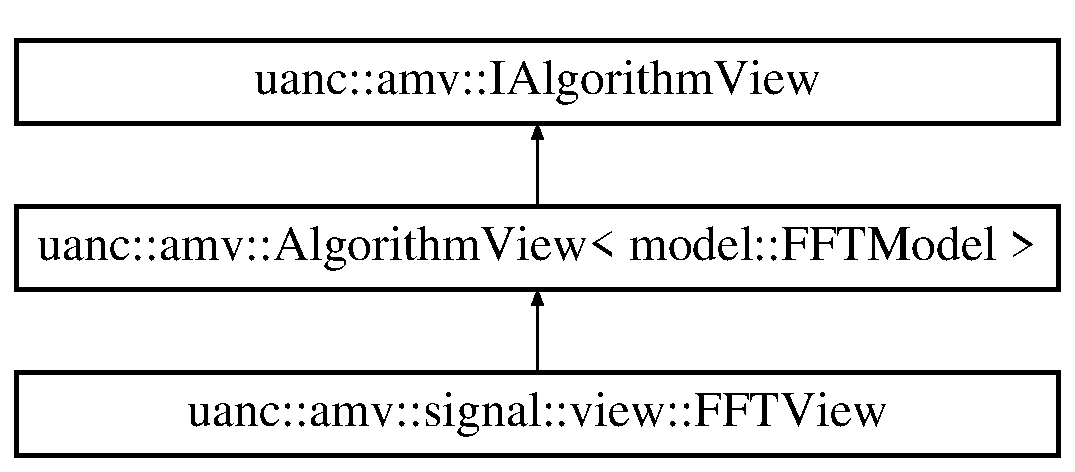
\includegraphics[height=3.000000cm]{classuanc_1_1amv_1_1signal_1_1view_1_1_f_f_t_view}
\end{center}
\end{figure}
\subsection*{Public Member Functions}
\begin{DoxyCompactItemize}
\item 
Q\+Widget $\ast$ \hyperlink{classuanc_1_1amv_1_1signal_1_1view_1_1_f_f_t_view_a774599a51059f878472cf72e2ce4b2b2}{produce\+Widget} () final
\begin{DoxyCompactList}\small\item\em Gets the complete widget. \end{DoxyCompactList}\item 
void \hyperlink{classuanc_1_1amv_1_1signal_1_1view_1_1_f_f_t_view_ae88ee6486f60d2d0a89c05f4d45546f7}{set\+Data} (std\+::shared\+\_\+ptr$<$ \hyperlink{classuanc_1_1amv_1_1signal_1_1model_1_1_f_f_t_model}{model\+::\+F\+F\+T\+Model} $>$ data) final
\begin{DoxyCompactList}\small\item\em This method applies the model data. \end{DoxyCompactList}\end{DoxyCompactItemize}


\subsection{Detailed Description}
Represents a \hyperlink{classuanc_1_1amv_1_1signal_1_1view_1_1_signal_view}{Signal\+View}. 

This represents a \hyperlink{classuanc_1_1amv_1_1signal_1_1view_1_1_signal_view}{Signal\+View} for F\+FT. It operates on an F\+F\+T\+Signal\+Model. It basically shows a plot of the F\+FT of the signal. 

\subsection{Member Function Documentation}
\index{uanc\+::amv\+::signal\+::view\+::\+F\+F\+T\+View@{uanc\+::amv\+::signal\+::view\+::\+F\+F\+T\+View}!produce\+Widget@{produce\+Widget}}
\index{produce\+Widget@{produce\+Widget}!uanc\+::amv\+::signal\+::view\+::\+F\+F\+T\+View@{uanc\+::amv\+::signal\+::view\+::\+F\+F\+T\+View}}
\subsubsection[{\texorpdfstring{produce\+Widget() final}{produceWidget() final}}]{\setlength{\rightskip}{0pt plus 5cm}Q\+Widget $\ast$ uanc\+::amv\+::signal\+::view\+::\+F\+F\+T\+View\+::produce\+Widget (
\begin{DoxyParamCaption}
{}
\end{DoxyParamCaption}
)\hspace{0.3cm}{\ttfamily [final]}, {\ttfamily [virtual]}}\hypertarget{classuanc_1_1amv_1_1signal_1_1view_1_1_f_f_t_view_a774599a51059f878472cf72e2ce4b2b2}{}\label{classuanc_1_1amv_1_1signal_1_1view_1_1_f_f_t_view_a774599a51059f878472cf72e2ce4b2b2}


Gets the complete widget. 

This function is used to retrieve the widget from the view. It gets used for integration the main application. It creates a Plotwidget inside of a Q\+Widget and passes this back.

\begin{DoxyReturn}{Returns}
The created widget.
\end{DoxyReturn}
This function is used to retrieve the widget from the view. It gets used for integration the main application. It creates a Plotwidget inside of a Q\+Widget and passes this back. Uses the singleton pattern to ensure the unique creation of the widget.

\begin{DoxyReturn}{Returns}
The created widget. 
\end{DoxyReturn}


Implements \hyperlink{classuanc_1_1amv_1_1_i_algorithm_view_ab9d06a0b43db57244868f10dae8e09e5}{uanc\+::amv\+::\+I\+Algorithm\+View}.

\index{uanc\+::amv\+::signal\+::view\+::\+F\+F\+T\+View@{uanc\+::amv\+::signal\+::view\+::\+F\+F\+T\+View}!set\+Data@{set\+Data}}
\index{set\+Data@{set\+Data}!uanc\+::amv\+::signal\+::view\+::\+F\+F\+T\+View@{uanc\+::amv\+::signal\+::view\+::\+F\+F\+T\+View}}
\subsubsection[{\texorpdfstring{set\+Data(std\+::shared\+\_\+ptr$<$ model\+::\+F\+F\+T\+Model $>$ data) final}{setData(std::shared_ptr< model::FFTModel > data) final}}]{\setlength{\rightskip}{0pt plus 5cm}void uanc\+::amv\+::signal\+::view\+::\+F\+F\+T\+View\+::set\+Data (
\begin{DoxyParamCaption}
\item[{std\+::shared\+\_\+ptr$<$ {\bf model\+::\+F\+F\+T\+Model} $>$}]{data}
\end{DoxyParamCaption}
)\hspace{0.3cm}{\ttfamily [final]}}\hypertarget{classuanc_1_1amv_1_1signal_1_1view_1_1_f_f_t_view_ae88ee6486f60d2d0a89c05f4d45546f7}{}\label{classuanc_1_1amv_1_1signal_1_1view_1_1_f_f_t_view_ae88ee6486f60d2d0a89c05f4d45546f7}


This method applies the model data. 

This method simply takes the passed data and places it inside of the view.


\begin{DoxyParams}{Parameters}
{\em data} & The applied data.\\
\hline
\end{DoxyParams}
This method simply takes the passed data and places it inside of the view at the appropriate places.


\begin{DoxyParams}{Parameters}
{\em data} & The applied data. \\
\hline
\end{DoxyParams}


The documentation for this class was generated from the following files\+:\begin{DoxyCompactItemize}
\item 
/home/kurt/\+Documents/\+Studium/\+Bachelor\+\_\+\+Praktikum/\+U\+A\+N\+C/\+Code/\+U\+A\+N\+C/amv/signal/view/\hyperlink{_f_f_t_view_8h}{F\+F\+T\+View.\+h}\item 
/home/kurt/\+Documents/\+Studium/\+Bachelor\+\_\+\+Praktikum/\+U\+A\+N\+C/\+Code/\+U\+A\+N\+C/amv/signal/view/\hyperlink{_f_f_t_view_8cpp}{F\+F\+T\+View.\+cpp}\end{DoxyCompactItemize}

\hypertarget{classuanc_1_1util_1_1_file_actor}{}\section{uanc\+:\+:util\+:\+:File\+Actor$<$ T $>$ Class Template Reference}
\label{classuanc_1_1util_1_1_file_actor}\index{uanc\+::util\+::\+File\+Actor$<$ T $>$@{uanc\+::util\+::\+File\+Actor$<$ T $>$}}


Simple \hyperlink{classuanc_1_1util_1_1_file_actor}{File\+Actor} class, which can operate on a file.  




{\ttfamily \#include $<$File\+Actor.\+h$>$}

\subsection*{Public Member Functions}
\begin{DoxyCompactItemize}
\item 
\hyperlink{classuanc_1_1util_1_1_file_actor_a2e2312c707145e6a3d47783fb8fe9fb0}{File\+Actor} (const std\+::string \&path)
\begin{DoxyCompactList}\small\item\em Basic constructor which saves a path string internally. \end{DoxyCompactList}\item 
virtual std\+::shared\+\_\+ptr$<$ T $>$ \hyperlink{classuanc_1_1util_1_1_file_actor_ad2db7584c9332a4d8376ccf6276ec301}{load\+Data} ()=0
\begin{DoxyCompactList}\small\item\em This method should load the file from the plate. \end{DoxyCompactList}\item 
virtual void \hyperlink{classuanc_1_1util_1_1_file_actor_aee5e36b37c46dda87f0499fc7b9e4b0d}{save\+Data} (std\+::shared\+\_\+ptr$<$ T $>$ source)=0
\begin{DoxyCompactList}\small\item\em This method should save a file to the plate. \end{DoxyCompactList}\end{DoxyCompactItemize}
\subsection*{Protected Member Functions}
\begin{DoxyCompactItemize}
\item 
std\+::string \hyperlink{classuanc_1_1util_1_1_file_actor_a9d2cae5553ce72cac745a46a25a946dc}{get\+Path} ()
\begin{DoxyCompactList}\small\item\em This method returns the path to the caller. \end{DoxyCompactList}\end{DoxyCompactItemize}


\subsection{Detailed Description}
\subsubsection*{template$<$typename T$>$\\*
class uanc\+::util\+::\+File\+Actor$<$ T $>$}

Simple \hyperlink{classuanc_1_1util_1_1_file_actor}{File\+Actor} class, which can operate on a file. 

This class can be used to write to a file and save something to that file of type S


\begin{DoxyTemplParams}{Template Parameters}
{\em T} & the type of object the file actor can handle \\
\hline
\end{DoxyTemplParams}


\subsection{Constructor \& Destructor Documentation}
\index{uanc\+::util\+::\+File\+Actor@{uanc\+::util\+::\+File\+Actor}!File\+Actor@{File\+Actor}}
\index{File\+Actor@{File\+Actor}!uanc\+::util\+::\+File\+Actor@{uanc\+::util\+::\+File\+Actor}}
\subsubsection[{\texorpdfstring{File\+Actor(const std\+::string \&path)}{FileActor(const std::string &path)}}]{\setlength{\rightskip}{0pt plus 5cm}template$<$typename T$>$ {\bf uanc\+::util\+::\+File\+Actor}$<$ T $>$\+::{\bf File\+Actor} (
\begin{DoxyParamCaption}
\item[{const std\+::string \&}]{path}
\end{DoxyParamCaption}
)\hspace{0.3cm}{\ttfamily [inline]}}\hypertarget{classuanc_1_1util_1_1_file_actor_a2e2312c707145e6a3d47783fb8fe9fb0}{}\label{classuanc_1_1util_1_1_file_actor_a2e2312c707145e6a3d47783fb8fe9fb0}


Basic constructor which saves a path string internally. 

This constructor just save the passed string internally.


\begin{DoxyParams}{Parameters}
{\em path} & The path to the acted file \\
\hline
\end{DoxyParams}


\subsection{Member Function Documentation}
\index{uanc\+::util\+::\+File\+Actor@{uanc\+::util\+::\+File\+Actor}!get\+Path@{get\+Path}}
\index{get\+Path@{get\+Path}!uanc\+::util\+::\+File\+Actor@{uanc\+::util\+::\+File\+Actor}}
\subsubsection[{\texorpdfstring{get\+Path()}{getPath()}}]{\setlength{\rightskip}{0pt plus 5cm}template$<$typename T$>$ std\+::string {\bf uanc\+::util\+::\+File\+Actor}$<$ T $>$\+::get\+Path (
\begin{DoxyParamCaption}
{}
\end{DoxyParamCaption}
)\hspace{0.3cm}{\ttfamily [inline]}, {\ttfamily [protected]}}\hypertarget{classuanc_1_1util_1_1_file_actor_a9d2cae5553ce72cac745a46a25a946dc}{}\label{classuanc_1_1util_1_1_file_actor_a9d2cae5553ce72cac745a46a25a946dc}


This method returns the path to the caller. 

This method can be used to obtain the inner saved path.

\begin{DoxyReturn}{Returns}
the path to the file 
\end{DoxyReturn}
\index{uanc\+::util\+::\+File\+Actor@{uanc\+::util\+::\+File\+Actor}!load\+Data@{load\+Data}}
\index{load\+Data@{load\+Data}!uanc\+::util\+::\+File\+Actor@{uanc\+::util\+::\+File\+Actor}}
\subsubsection[{\texorpdfstring{load\+Data()=0}{loadData()=0}}]{\setlength{\rightskip}{0pt plus 5cm}template$<$typename T$>$ virtual std\+::shared\+\_\+ptr$<$T$>$ {\bf uanc\+::util\+::\+File\+Actor}$<$ T $>$\+::load\+Data (
\begin{DoxyParamCaption}
{}
\end{DoxyParamCaption}
)\hspace{0.3cm}{\ttfamily [pure virtual]}}\hypertarget{classuanc_1_1util_1_1_file_actor_ad2db7584c9332a4d8376ccf6276ec301}{}\label{classuanc_1_1util_1_1_file_actor_ad2db7584c9332a4d8376ccf6276ec301}


This method should load the file from the plate. 

This method should return the loaded T

\begin{DoxyReturn}{Returns}
the loaded T 
\end{DoxyReturn}


Implemented in \hyperlink{classuanc_1_1util_1_1_signal_file_actor_a2069e33e03ebc63eac2080d40f863ce3}{uanc\+::util\+::\+Signal\+File\+Actor}, and \hyperlink{classuanc_1_1util_1_1_dummy_actor_ae2912157674c282f5436f27ddbfcf8cc}{uanc\+::util\+::\+Dummy\+Actor}.

\index{uanc\+::util\+::\+File\+Actor@{uanc\+::util\+::\+File\+Actor}!save\+Data@{save\+Data}}
\index{save\+Data@{save\+Data}!uanc\+::util\+::\+File\+Actor@{uanc\+::util\+::\+File\+Actor}}
\subsubsection[{\texorpdfstring{save\+Data(std\+::shared\+\_\+ptr$<$ T $>$ source)=0}{saveData(std::shared_ptr< T > source)=0}}]{\setlength{\rightskip}{0pt plus 5cm}template$<$typename T$>$ virtual void {\bf uanc\+::util\+::\+File\+Actor}$<$ T $>$\+::save\+Data (
\begin{DoxyParamCaption}
\item[{std\+::shared\+\_\+ptr$<$ T $>$}]{source}
\end{DoxyParamCaption}
)\hspace{0.3cm}{\ttfamily [pure virtual]}}\hypertarget{classuanc_1_1util_1_1_file_actor_aee5e36b37c46dda87f0499fc7b9e4b0d}{}\label{classuanc_1_1util_1_1_file_actor_aee5e36b37c46dda87f0499fc7b9e4b0d}


This method should save a file to the plate. 

This should method should save the passed T to the specified path.


\begin{DoxyParams}{Parameters}
{\em source} & The source to save \\
\hline
\end{DoxyParams}


Implemented in \hyperlink{classuanc_1_1util_1_1_signal_file_actor_a77695bd57923ec24ff78ec8361bcfca2}{uanc\+::util\+::\+Signal\+File\+Actor}, and \hyperlink{classuanc_1_1util_1_1_dummy_actor_a321ba3ff6c3718d56edb6efe961f8230}{uanc\+::util\+::\+Dummy\+Actor}.



The documentation for this class was generated from the following file\+:\begin{DoxyCompactItemize}
\item 
/home/kurt/\+Documents/\+Studium/\+Bachelor\+\_\+\+Praktikum/\+U\+A\+N\+C/\+Code/\+U\+A\+N\+C/util/\hyperlink{_file_actor_8h}{File\+Actor.\+h}\end{DoxyCompactItemize}

\hypertarget{classuanc_1_1util_1_1_global_settings}{}\section{uanc\+:\+:util\+:\+:Global\+Settings Class Reference}
\label{classuanc_1_1util_1_1_global_settings}\index{uanc\+::util\+::\+Global\+Settings@{uanc\+::util\+::\+Global\+Settings}}


{\ttfamily \#include $<$Global\+Settings.\+h$>$}

\subsection*{Static Public Member Functions}
\begin{DoxyCompactItemize}
\item 
static \hyperlink{classuanc_1_1util_1_1_global_settings}{Global\+Settings} $\ast$ \hyperlink{classuanc_1_1util_1_1_global_settings_a346f903079cd632e18278d30f03a1fac}{get} ()
\begin{DoxyCompactList}\small\item\em The default Constructor. \end{DoxyCompactList}\end{DoxyCompactItemize}
\subsection*{Public Attributes}
\begin{DoxyCompactItemize}
\item 
int \hyperlink{classuanc_1_1util_1_1_global_settings_aa44f491fb5835682da35431cac26ab28}{current\+Index} = 0
\end{DoxyCompactItemize}
\subsection*{Static Public Attributes}
\begin{DoxyCompactItemize}
\item 
static \hyperlink{classuanc_1_1util_1_1_global_settings}{Global\+Settings} $\ast$ \hyperlink{classuanc_1_1util_1_1_global_settings_a4edfe7df393a7c61477aec88f61419b5}{global\+Settings} = nullptr
\end{DoxyCompactItemize}


\subsection{Member Function Documentation}
\index{uanc\+::util\+::\+Global\+Settings@{uanc\+::util\+::\+Global\+Settings}!get@{get}}
\index{get@{get}!uanc\+::util\+::\+Global\+Settings@{uanc\+::util\+::\+Global\+Settings}}
\subsubsection[{\texorpdfstring{get()}{get()}}]{\setlength{\rightskip}{0pt plus 5cm}static {\bf Global\+Settings}$\ast$ uanc\+::util\+::\+Global\+Settings\+::get (
\begin{DoxyParamCaption}
{}
\end{DoxyParamCaption}
)\hspace{0.3cm}{\ttfamily [inline]}, {\ttfamily [static]}}\hypertarget{classuanc_1_1util_1_1_global_settings_a346f903079cd632e18278d30f03a1fac}{}\label{classuanc_1_1util_1_1_global_settings_a346f903079cd632e18278d30f03a1fac}


The default Constructor. 



\subsection{Member Data Documentation}
\index{uanc\+::util\+::\+Global\+Settings@{uanc\+::util\+::\+Global\+Settings}!current\+Index@{current\+Index}}
\index{current\+Index@{current\+Index}!uanc\+::util\+::\+Global\+Settings@{uanc\+::util\+::\+Global\+Settings}}
\subsubsection[{\texorpdfstring{current\+Index}{currentIndex}}]{\setlength{\rightskip}{0pt plus 5cm}int uanc\+::util\+::\+Global\+Settings\+::current\+Index = 0}\hypertarget{classuanc_1_1util_1_1_global_settings_aa44f491fb5835682da35431cac26ab28}{}\label{classuanc_1_1util_1_1_global_settings_aa44f491fb5835682da35431cac26ab28}
\index{uanc\+::util\+::\+Global\+Settings@{uanc\+::util\+::\+Global\+Settings}!global\+Settings@{global\+Settings}}
\index{global\+Settings@{global\+Settings}!uanc\+::util\+::\+Global\+Settings@{uanc\+::util\+::\+Global\+Settings}}
\subsubsection[{\texorpdfstring{global\+Settings}{globalSettings}}]{\setlength{\rightskip}{0pt plus 5cm}{\bf Global\+Settings} $\ast$ Global\+Settings\+::global\+Settings = nullptr\hspace{0.3cm}{\ttfamily [static]}}\hypertarget{classuanc_1_1util_1_1_global_settings_a4edfe7df393a7c61477aec88f61419b5}{}\label{classuanc_1_1util_1_1_global_settings_a4edfe7df393a7c61477aec88f61419b5}


The documentation for this class was generated from the following files\+:\begin{DoxyCompactItemize}
\item 
/ext/local/\+University/\+B\+P/\+Git/\+U\+A\+N\+C/\+Code/\+U\+A\+N\+C/util/\hyperlink{_global_settings_8h}{Global\+Settings.\+h}\item 
/ext/local/\+University/\+B\+P/\+Git/\+U\+A\+N\+C/\+Code/\+U\+A\+N\+C/\hyperlink{main_8cpp}{main.\+cpp}\end{DoxyCompactItemize}

\hypertarget{classuanc_1_1gui_1_1_global_settings_bar}{}\section{uanc\+:\+:gui\+:\+:Global\+Settings\+Bar Class Reference}
\label{classuanc_1_1gui_1_1_global_settings_bar}\index{uanc\+::gui\+::\+Global\+Settings\+Bar@{uanc\+::gui\+::\+Global\+Settings\+Bar}}


{\ttfamily \#include $<$Global\+Settings\+Bar.\+h$>$}

Inheritance diagram for uanc\+:\+:gui\+:\+:Global\+Settings\+Bar\+:\begin{figure}[H]
\begin{center}
\leavevmode
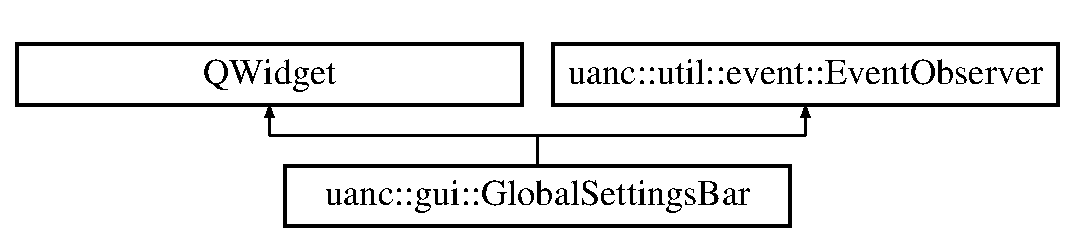
\includegraphics[height=2.000000cm]{classuanc_1_1gui_1_1_global_settings_bar}
\end{center}
\end{figure}
\subsection*{Public Slots}
\begin{DoxyCompactItemize}
\item 
void \hyperlink{classuanc_1_1gui_1_1_global_settings_bar_a76c5c5bac6194b489297d75544df830b}{changed\+View} (int index)
\end{DoxyCompactItemize}
\subsection*{Public Member Functions}
\begin{DoxyCompactItemize}
\item 
\hyperlink{classuanc_1_1gui_1_1_global_settings_bar_a7b4d8ddaae819768287db58572982718}{Global\+Settings\+Bar} (int has\+Right)
\item 
\hyperlink{classuanc_1_1gui_1_1_global_settings_bar_a26cb9645d1f50fc7f3be71f15720e43e}{$\sim$\+Global\+Settings\+Bar} ()
\item 
void \hyperlink{classuanc_1_1gui_1_1_global_settings_bar_a780fabb890235753ff90c1403638c47d}{triggered} (\hyperlink{namespaceuanc_1_1util_1_1event_a63f690675589114db9c6bcbe6f1088a4}{Events} event, \hyperlink{classuanc_1_1util_1_1event_1_1_event_container}{Event\+Container} data) final
\item 
void \hyperlink{classuanc_1_1gui_1_1_global_settings_bar_a3466ddea370d0c7e4c1ae7062092bc5a}{changed\+Channel} (int index)
\end{DoxyCompactItemize}
\subsection*{Additional Inherited Members}


\subsection{Detailed Description}
This class represents the global settings bar. It fires an event so that all views can change. 

\subsection{Constructor \& Destructor Documentation}
\index{uanc\+::gui\+::\+Global\+Settings\+Bar@{uanc\+::gui\+::\+Global\+Settings\+Bar}!Global\+Settings\+Bar@{Global\+Settings\+Bar}}
\index{Global\+Settings\+Bar@{Global\+Settings\+Bar}!uanc\+::gui\+::\+Global\+Settings\+Bar@{uanc\+::gui\+::\+Global\+Settings\+Bar}}
\subsubsection[{\texorpdfstring{Global\+Settings\+Bar(int has\+Right)}{GlobalSettingsBar(int hasRight)}}]{\setlength{\rightskip}{0pt plus 5cm}uanc\+::gui\+::\+Global\+Settings\+Bar\+::\+Global\+Settings\+Bar (
\begin{DoxyParamCaption}
\item[{int}]{has\+Right}
\end{DoxyParamCaption}
)\hspace{0.3cm}{\ttfamily [inline]}}\hypertarget{classuanc_1_1gui_1_1_global_settings_bar_a7b4d8ddaae819768287db58572982718}{}\label{classuanc_1_1gui_1_1_global_settings_bar_a7b4d8ddaae819768287db58572982718}
Default constructor for the signal view change bar. \index{uanc\+::gui\+::\+Global\+Settings\+Bar@{uanc\+::gui\+::\+Global\+Settings\+Bar}!````~Global\+Settings\+Bar@{$\sim$\+Global\+Settings\+Bar}}
\index{````~Global\+Settings\+Bar@{$\sim$\+Global\+Settings\+Bar}!uanc\+::gui\+::\+Global\+Settings\+Bar@{uanc\+::gui\+::\+Global\+Settings\+Bar}}
\subsubsection[{\texorpdfstring{$\sim$\+Global\+Settings\+Bar()}{~GlobalSettingsBar()}}]{\setlength{\rightskip}{0pt plus 5cm}uanc\+::gui\+::\+Global\+Settings\+Bar\+::$\sim$\+Global\+Settings\+Bar (
\begin{DoxyParamCaption}
{}
\end{DoxyParamCaption}
)\hspace{0.3cm}{\ttfamily [inline]}}\hypertarget{classuanc_1_1gui_1_1_global_settings_bar_a26cb9645d1f50fc7f3be71f15720e43e}{}\label{classuanc_1_1gui_1_1_global_settings_bar_a26cb9645d1f50fc7f3be71f15720e43e}


\subsection{Member Function Documentation}
\index{uanc\+::gui\+::\+Global\+Settings\+Bar@{uanc\+::gui\+::\+Global\+Settings\+Bar}!changed\+Channel@{changed\+Channel}}
\index{changed\+Channel@{changed\+Channel}!uanc\+::gui\+::\+Global\+Settings\+Bar@{uanc\+::gui\+::\+Global\+Settings\+Bar}}
\subsubsection[{\texorpdfstring{changed\+Channel(int index)}{changedChannel(int index)}}]{\setlength{\rightskip}{0pt plus 5cm}void uanc\+::gui\+::\+Global\+Settings\+Bar\+::changed\+Channel (
\begin{DoxyParamCaption}
\item[{int}]{index}
\end{DoxyParamCaption}
)\hspace{0.3cm}{\ttfamily [inline]}}\hypertarget{classuanc_1_1gui_1_1_global_settings_bar_a3466ddea370d0c7e4c1ae7062092bc5a}{}\label{classuanc_1_1gui_1_1_global_settings_bar_a3466ddea370d0c7e4c1ae7062092bc5a}
Slot if channel changed \index{uanc\+::gui\+::\+Global\+Settings\+Bar@{uanc\+::gui\+::\+Global\+Settings\+Bar}!changed\+View@{changed\+View}}
\index{changed\+View@{changed\+View}!uanc\+::gui\+::\+Global\+Settings\+Bar@{uanc\+::gui\+::\+Global\+Settings\+Bar}}
\subsubsection[{\texorpdfstring{changed\+View}{changedView}}]{\setlength{\rightskip}{0pt plus 5cm}void uanc\+::gui\+::\+Global\+Settings\+Bar\+::changed\+View (
\begin{DoxyParamCaption}
\item[{int}]{index}
\end{DoxyParamCaption}
)\hspace{0.3cm}{\ttfamily [inline]}, {\ttfamily [slot]}}\hypertarget{classuanc_1_1gui_1_1_global_settings_bar_a76c5c5bac6194b489297d75544df830b}{}\label{classuanc_1_1gui_1_1_global_settings_bar_a76c5c5bac6194b489297d75544df830b}
Slot if the view changed \index{uanc\+::gui\+::\+Global\+Settings\+Bar@{uanc\+::gui\+::\+Global\+Settings\+Bar}!triggered@{triggered}}
\index{triggered@{triggered}!uanc\+::gui\+::\+Global\+Settings\+Bar@{uanc\+::gui\+::\+Global\+Settings\+Bar}}
\subsubsection[{\texorpdfstring{triggered(\+Events event, Event\+Container data) final}{triggered(Events event, EventContainer data) final}}]{\setlength{\rightskip}{0pt plus 5cm}void uanc\+::gui\+::\+Global\+Settings\+Bar\+::triggered (
\begin{DoxyParamCaption}
\item[{{\bf Events}}]{event, }
\item[{{\bf Event\+Container}}]{data}
\end{DoxyParamCaption}
)\hspace{0.3cm}{\ttfamily [inline]}, {\ttfamily [final]}, {\ttfamily [virtual]}}\hypertarget{classuanc_1_1gui_1_1_global_settings_bar_a780fabb890235753ff90c1403638c47d}{}\label{classuanc_1_1gui_1_1_global_settings_bar_a780fabb890235753ff90c1403638c47d}
This method gets called when one of the events was triggered. 

Implements \hyperlink{classuanc_1_1util_1_1event_1_1_event_observer_af1640e34db3379eaba8c817a92199807}{uanc\+::util\+::event\+::\+Event\+Observer}.



The documentation for this class was generated from the following file\+:\begin{DoxyCompactItemize}
\item 
/ext/local/\+University/\+B\+P/\+Git/\+U\+A\+N\+C/\+Code/\+U\+A\+N\+C/gui/\hyperlink{_global_settings_bar_8h}{Global\+Settings\+Bar.\+h}\end{DoxyCompactItemize}

\hypertarget{classuanc_1_1amv_1_1signal_1_1view_1_1_heat_view}{}\section{uanc\+:\+:amv\+:\+:signal\+:\+:view\+:\+:Heat\+View Class Reference}
\label{classuanc_1_1amv_1_1signal_1_1view_1_1_heat_view}\index{uanc\+::amv\+::signal\+::view\+::\+Heat\+View@{uanc\+::amv\+::signal\+::view\+::\+Heat\+View}}


{\ttfamily \#include $<$Heat\+View.\+h$>$}

Inheritance diagram for uanc\+:\+:amv\+:\+:signal\+:\+:view\+:\+:Heat\+View\+:\begin{figure}[H]
\begin{center}
\leavevmode
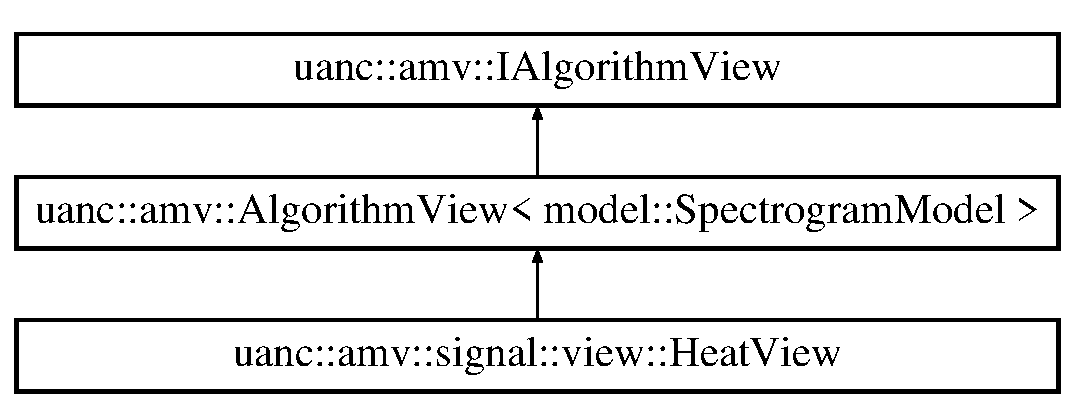
\includegraphics[height=3.000000cm]{classuanc_1_1amv_1_1signal_1_1view_1_1_heat_view}
\end{center}
\end{figure}
\subsection*{Public Member Functions}
\begin{DoxyCompactItemize}
\item 
Q\+Widget $\ast$ \hyperlink{classuanc_1_1amv_1_1signal_1_1view_1_1_heat_view_a93ac20354fa17ab67e368e324f240c9a}{produce\+Widget} () final
\begin{DoxyCompactList}\small\item\em Produces the widget. \end{DoxyCompactList}\item 
void \hyperlink{classuanc_1_1amv_1_1signal_1_1view_1_1_heat_view_a0c6ded83c8aefdf05ff1abd8344763df}{set\+Data} (std\+::shared\+\_\+ptr$<$ \hyperlink{classuanc_1_1amv_1_1signal_1_1model_1_1_spectrogram_model}{model\+::\+Spectrogram\+Model} $>$ data) final
\begin{DoxyCompactList}\small\item\em This method applies the model data. \end{DoxyCompactList}\end{DoxyCompactItemize}


\subsection{Member Function Documentation}
\index{uanc\+::amv\+::signal\+::view\+::\+Heat\+View@{uanc\+::amv\+::signal\+::view\+::\+Heat\+View}!produce\+Widget@{produce\+Widget}}
\index{produce\+Widget@{produce\+Widget}!uanc\+::amv\+::signal\+::view\+::\+Heat\+View@{uanc\+::amv\+::signal\+::view\+::\+Heat\+View}}
\subsubsection[{\texorpdfstring{produce\+Widget() final}{produceWidget() final}}]{\setlength{\rightskip}{0pt plus 5cm}Q\+Widget$\ast$ uanc\+::amv\+::signal\+::view\+::\+Heat\+View\+::produce\+Widget (
\begin{DoxyParamCaption}
{}
\end{DoxyParamCaption}
)\hspace{0.3cm}{\ttfamily [inline]}, {\ttfamily [final]}, {\ttfamily [virtual]}}\hypertarget{classuanc_1_1amv_1_1signal_1_1view_1_1_heat_view_a93ac20354fa17ab67e368e324f240c9a}{}\label{classuanc_1_1amv_1_1signal_1_1view_1_1_heat_view_a93ac20354fa17ab67e368e324f240c9a}


Produces the widget. 

This function is used to produce the widget from the view. It gets used for integration the main application

\begin{DoxyReturn}{Returns}
The created widget. 
\end{DoxyReturn}


Implements \hyperlink{classuanc_1_1amv_1_1_i_algorithm_view_ab9d06a0b43db57244868f10dae8e09e5}{uanc\+::amv\+::\+I\+Algorithm\+View}.

\index{uanc\+::amv\+::signal\+::view\+::\+Heat\+View@{uanc\+::amv\+::signal\+::view\+::\+Heat\+View}!set\+Data@{set\+Data}}
\index{set\+Data@{set\+Data}!uanc\+::amv\+::signal\+::view\+::\+Heat\+View@{uanc\+::amv\+::signal\+::view\+::\+Heat\+View}}
\subsubsection[{\texorpdfstring{set\+Data(std\+::shared\+\_\+ptr$<$ model\+::\+Spectrogram\+Model $>$ data) final}{setData(std::shared_ptr< model::SpectrogramModel > data) final}}]{\setlength{\rightskip}{0pt plus 5cm}void uanc\+::amv\+::signal\+::view\+::\+Heat\+View\+::set\+Data (
\begin{DoxyParamCaption}
\item[{std\+::shared\+\_\+ptr$<$ {\bf model\+::\+Spectrogram\+Model} $>$}]{data}
\end{DoxyParamCaption}
)\hspace{0.3cm}{\ttfamily [inline]}, {\ttfamily [final]}, {\ttfamily [virtual]}}\hypertarget{classuanc_1_1amv_1_1signal_1_1view_1_1_heat_view_a0c6ded83c8aefdf05ff1abd8344763df}{}\label{classuanc_1_1amv_1_1signal_1_1view_1_1_heat_view_a0c6ded83c8aefdf05ff1abd8344763df}


This method applies the model data. 

This method simply takes the passed data and places it inside of the view at the appropriate places.


\begin{DoxyParams}{Parameters}
{\em data} & The applied data. \\
\hline
\end{DoxyParams}


Implements \hyperlink{classuanc_1_1amv_1_1_algorithm_view_ad656cf5223a66a942441ee39f44f65a3}{uanc\+::amv\+::\+Algorithm\+View$<$ model\+::\+Spectrogram\+Model $>$}.



The documentation for this class was generated from the following file\+:\begin{DoxyCompactItemize}
\item 
/home/kurt/\+Documents/\+Studium/\+Bachelor\+\_\+\+Praktikum/\+U\+A\+N\+C/\+Code/\+U\+A\+N\+C/amv/signal/view/\hyperlink{_heat_view_8h}{Heat\+View.\+h}\end{DoxyCompactItemize}

\hypertarget{classuanc_1_1gui_1_1_heat_widget}{}\section{uanc\+:\+:gui\+:\+:Heat\+Widget Class Reference}
\label{classuanc_1_1gui_1_1_heat_widget}\index{uanc\+::gui\+::\+Heat\+Widget@{uanc\+::gui\+::\+Heat\+Widget}}


{\ttfamily \#include $<$Heat\+Widget.\+h$>$}

Inheritance diagram for uanc\+:\+:gui\+:\+:Heat\+Widget\+:\begin{figure}[H]
\begin{center}
\leavevmode
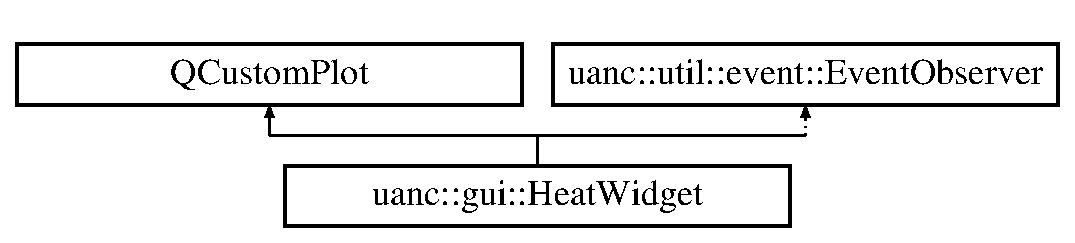
\includegraphics[height=2.000000cm]{classuanc_1_1gui_1_1_heat_widget}
\end{center}
\end{figure}
\subsection*{Public Member Functions}
\begin{DoxyCompactItemize}
\item 
\hyperlink{classuanc_1_1gui_1_1_heat_widget_ad2ab17fd2d3cf74fb5f6d973e5689f74}{Heat\+Widget} ()
\begin{DoxyCompactList}\small\item\em Constructor of \hyperlink{classuanc_1_1gui_1_1_control}{Control} class. \end{DoxyCompactList}\item 
void \hyperlink{classuanc_1_1gui_1_1_heat_widget_aabf936a98a00a3934278cd490be16793}{set\+Data} (std\+::shared\+\_\+ptr$<$ \hyperlink{classuanc_1_1amv_1_1signal_1_1model_1_1_spectrogram_model}{Spectrogram\+Model} $>$ data)
\begin{DoxyCompactList}\small\item\em change channel to spectrogram \end{DoxyCompactList}\item 
void \hyperlink{classuanc_1_1gui_1_1_heat_widget_a3d97fc4b902d3a90a197124b190deebd}{config\+Plot} (std\+::shared\+\_\+ptr$<$ Aquila\+::\+Spectrogram $>$ spectrogramm)
\begin{DoxyCompactList}\small\item\em plots spectogram \end{DoxyCompactList}\item 
void \hyperlink{classuanc_1_1gui_1_1_heat_widget_afe92e65ebf7d607ef7e1d40aaaa6131a}{triggered} (\hyperlink{namespaceuanc_1_1util_1_1event_a63f690675589114db9c6bcbe6f1088a4}{Events} event, \hyperlink{classuanc_1_1util_1_1event_1_1_event_container}{Event\+Container} data)
\begin{DoxyCompactList}\small\item\em starts channelswitch when triggered by event \end{DoxyCompactList}\end{DoxyCompactItemize}


\subsection{Constructor \& Destructor Documentation}
\index{uanc\+::gui\+::\+Heat\+Widget@{uanc\+::gui\+::\+Heat\+Widget}!Heat\+Widget@{Heat\+Widget}}
\index{Heat\+Widget@{Heat\+Widget}!uanc\+::gui\+::\+Heat\+Widget@{uanc\+::gui\+::\+Heat\+Widget}}
\subsubsection[{\texorpdfstring{Heat\+Widget()}{HeatWidget()}}]{\setlength{\rightskip}{0pt plus 5cm}uanc\+::gui\+::\+Heat\+Widget\+::\+Heat\+Widget (
\begin{DoxyParamCaption}
{}
\end{DoxyParamCaption}
)\hspace{0.3cm}{\ttfamily [inline]}}\hypertarget{classuanc_1_1gui_1_1_heat_widget_ad2ab17fd2d3cf74fb5f6d973e5689f74}{}\label{classuanc_1_1gui_1_1_heat_widget_ad2ab17fd2d3cf74fb5f6d973e5689f74}


Constructor of \hyperlink{classuanc_1_1gui_1_1_control}{Control} class. 



\subsection{Member Function Documentation}
\index{uanc\+::gui\+::\+Heat\+Widget@{uanc\+::gui\+::\+Heat\+Widget}!config\+Plot@{config\+Plot}}
\index{config\+Plot@{config\+Plot}!uanc\+::gui\+::\+Heat\+Widget@{uanc\+::gui\+::\+Heat\+Widget}}
\subsubsection[{\texorpdfstring{config\+Plot(std\+::shared\+\_\+ptr$<$ Aquila\+::\+Spectrogram $>$ spectrogramm)}{configPlot(std::shared_ptr< Aquila::Spectrogram > spectrogramm)}}]{\setlength{\rightskip}{0pt plus 5cm}void uanc\+::gui\+::\+Heat\+Widget\+::config\+Plot (
\begin{DoxyParamCaption}
\item[{std\+::shared\+\_\+ptr$<$ Aquila\+::\+Spectrogram $>$}]{spectrogramm}
\end{DoxyParamCaption}
)\hspace{0.3cm}{\ttfamily [inline]}}\hypertarget{classuanc_1_1gui_1_1_heat_widget_a3d97fc4b902d3a90a197124b190deebd}{}\label{classuanc_1_1gui_1_1_heat_widget_a3d97fc4b902d3a90a197124b190deebd}


plots spectogram 

configures the changes to show spectrogram


\begin{DoxyParams}{Parameters}
{\em spectrogramm} & given spectrogram \\
\hline
\end{DoxyParams}
\index{uanc\+::gui\+::\+Heat\+Widget@{uanc\+::gui\+::\+Heat\+Widget}!set\+Data@{set\+Data}}
\index{set\+Data@{set\+Data}!uanc\+::gui\+::\+Heat\+Widget@{uanc\+::gui\+::\+Heat\+Widget}}
\subsubsection[{\texorpdfstring{set\+Data(std\+::shared\+\_\+ptr$<$ Spectrogram\+Model $>$ data)}{setData(std::shared_ptr< SpectrogramModel > data)}}]{\setlength{\rightskip}{0pt plus 5cm}void uanc\+::gui\+::\+Heat\+Widget\+::set\+Data (
\begin{DoxyParamCaption}
\item[{std\+::shared\+\_\+ptr$<$ {\bf Spectrogram\+Model} $>$}]{data}
\end{DoxyParamCaption}
)\hspace{0.3cm}{\ttfamily [inline]}}\hypertarget{classuanc_1_1gui_1_1_heat_widget_aabf936a98a00a3934278cd490be16793}{}\label{classuanc_1_1gui_1_1_heat_widget_aabf936a98a00a3934278cd490be16793}


change channel to spectrogram 


\begin{DoxyParams}{Parameters}
{\em data} & given spectrogram data \\
\hline
\end{DoxyParams}
\index{uanc\+::gui\+::\+Heat\+Widget@{uanc\+::gui\+::\+Heat\+Widget}!triggered@{triggered}}
\index{triggered@{triggered}!uanc\+::gui\+::\+Heat\+Widget@{uanc\+::gui\+::\+Heat\+Widget}}
\subsubsection[{\texorpdfstring{triggered(\+Events event, Event\+Container data)}{triggered(Events event, EventContainer data)}}]{\setlength{\rightskip}{0pt plus 5cm}void uanc\+::gui\+::\+Heat\+Widget\+::triggered (
\begin{DoxyParamCaption}
\item[{{\bf Events}}]{event, }
\item[{{\bf Event\+Container}}]{data}
\end{DoxyParamCaption}
)\hspace{0.3cm}{\ttfamily [inline]}, {\ttfamily [virtual]}}\hypertarget{classuanc_1_1gui_1_1_heat_widget_afe92e65ebf7d607ef7e1d40aaaa6131a}{}\label{classuanc_1_1gui_1_1_heat_widget_afe92e65ebf7d607ef7e1d40aaaa6131a}


starts channelswitch when triggered by event 


\begin{DoxyParams}{Parameters}
{\em event} & given event \\
\hline
{\em data} & given events \\
\hline
\end{DoxyParams}


Implements \hyperlink{classuanc_1_1util_1_1event_1_1_event_observer_af1640e34db3379eaba8c817a92199807}{uanc\+::util\+::event\+::\+Event\+Observer}.



The documentation for this class was generated from the following file\+:\begin{DoxyCompactItemize}
\item 
/ext/local/\+University/\+B\+P/\+Git/\+U\+A\+N\+C/\+Code/\+U\+A\+N\+C/gui/\hyperlink{_heat_widget_8h}{Heat\+Widget.\+h}\end{DoxyCompactItemize}

\hypertarget{classuanc_1_1amv_1_1_i_algorithm}{}\section{uanc\+:\+:amv\+:\+:I\+Algorithm Class Reference}
\label{classuanc_1_1amv_1_1_i_algorithm}\index{uanc\+::amv\+::\+I\+Algorithm@{uanc\+::amv\+::\+I\+Algorithm}}


General interface for any algorithm.  




{\ttfamily \#include $<$I\+Algorithm.\+h$>$}

Inheritance diagram for uanc\+:\+:amv\+:\+:I\+Algorithm\+:\begin{figure}[H]
\begin{center}
\leavevmode
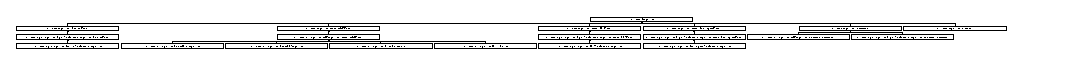
\includegraphics[height=0.429942cm]{classuanc_1_1amv_1_1_i_algorithm}
\end{center}
\end{figure}
\subsection*{Public Member Functions}
\begin{DoxyCompactItemize}
\item 
virtual \hyperlink{classuanc_1_1amv_1_1_i_algorithm}{I\+Algorithm} $\ast$ \hyperlink{classuanc_1_1amv_1_1_i_algorithm_af6fcbfa35f460363c2cc7e6134af8dc7}{clone} ()=0
\begin{DoxyCompactList}\small\item\em Clones the current instance. \end{DoxyCompactList}\item 
virtual void \hyperlink{classuanc_1_1amv_1_1_i_algorithm_a6f71d353db186306f5d4e191f0c15cc4}{fill\+View} ()=0
\begin{DoxyCompactList}\small\item\em Fills the view with the data. \end{DoxyCompactList}\item 
virtual std\+::string \hyperlink{classuanc_1_1amv_1_1_i_algorithm_a4935ab2fdacccf7df35d6fb596075edb}{get\+Name} ()=0
\begin{DoxyCompactList}\small\item\em Returns the name of the algorithm. \end{DoxyCompactList}\item 
virtual \hyperlink{classuanc_1_1amv_1_1_i_algorithm_view}{I\+Algorithm\+View} $\ast$ \hyperlink{classuanc_1_1amv_1_1_i_algorithm_ab1806c419a1e73adc149b7fb187d23d7}{get\+View} ()=0
\begin{DoxyCompactList}\small\item\em Gets a reference to the associated view. \end{DoxyCompactList}\item 
virtual void \hyperlink{classuanc_1_1amv_1_1_i_algorithm_a14dd1e42a421c48b8874e42933daa0b9}{process} (std\+::shared\+\_\+ptr$<$ \hyperlink{classuanc_1_1amv_1_1_inverted_model}{uanc\+::amv\+::\+Inverted\+Model} $>$ input)=0
\begin{DoxyCompactList}\small\item\em Processes the input signal model. \end{DoxyCompactList}\end{DoxyCompactItemize}


\subsection{Detailed Description}
General interface for any algorithm. 

This interface is used in the client code. Therefore it has no knowledge of the underlying model nor the view. It gets used for signal views as well as algorithm views. 

\subsection{Member Function Documentation}
\index{uanc\+::amv\+::\+I\+Algorithm@{uanc\+::amv\+::\+I\+Algorithm}!clone@{clone}}
\index{clone@{clone}!uanc\+::amv\+::\+I\+Algorithm@{uanc\+::amv\+::\+I\+Algorithm}}
\subsubsection[{\texorpdfstring{clone()=0}{clone()=0}}]{\setlength{\rightskip}{0pt plus 5cm}virtual {\bf I\+Algorithm}$\ast$ uanc\+::amv\+::\+I\+Algorithm\+::clone (
\begin{DoxyParamCaption}
{}
\end{DoxyParamCaption}
)\hspace{0.3cm}{\ttfamily [pure virtual]}}\hypertarget{classuanc_1_1amv_1_1_i_algorithm_af6fcbfa35f460363c2cc7e6134af8dc7}{}\label{classuanc_1_1amv_1_1_i_algorithm_af6fcbfa35f460363c2cc7e6134af8dc7}


Clones the current instance. 

This is basically the prototype pattern. It gets used to create an exact copy of the current instance.

\begin{DoxyReturn}{Returns}
The cloned algorithm. 
\end{DoxyReturn}


Implemented in \hyperlink{classuanc_1_1amv_1_1anc_1_1algorithm_1_1_inverse_f_f_t_algorithm_abb8ee8a2ba58c14cf2a138657f3cc211}{uanc\+::amv\+::anc\+::algorithm\+::\+Inverse\+F\+F\+T\+Algorithm}, \hyperlink{classuanc_1_1amv_1_1signal_1_1algorithm_1_1_f_f_t_transformation_algorithm_a8829e808c4bd019564c9ba874e7b7bf0}{uanc\+::amv\+::signal\+::algorithm\+::\+F\+F\+T\+Transformation\+Algorithm}, \hyperlink{classuanc_1_1amv_1_1anc_1_1algorithm_1_1_spline_interpolation_a43063277ff720c71b932ee29673b568f}{uanc\+::amv\+::anc\+::algorithm\+::\+Spline\+Interpolation}, \hyperlink{classuanc_1_1amv_1_1anc_1_1algorithm_1_1_inverse_direct_algorithm_adce538c00ba00237ba29d725abaae764}{uanc\+::amv\+::anc\+::algorithm\+::\+Inverse\+Direct\+Algorithm}, \hyperlink{classuanc_1_1amv_1_1anc_1_1algorithm_1_1_linear_extrapolation_adbd3916228ea66603c4c5362f3392548}{uanc\+::amv\+::anc\+::algorithm\+::\+Linear\+Extrapolation}, \hyperlink{classuanc_1_1amv_1_1signal_1_1algorithm_1_1_spectrogram_transformation_algorithm_a6efc3617627883a6d2acc52e582dd5a3}{uanc\+::amv\+::signal\+::algorithm\+::\+Spectrogram\+Transformation\+Algorithm}, and \hyperlink{classuanc_1_1amv_1_1signal_1_1algorithm_1_1_identity_transformation_algorithm_a863e785131c7e4f7d41d403a7fb4526d}{uanc\+::amv\+::signal\+::algorithm\+::\+Identity\+Transformation\+Algorithm}.

\index{uanc\+::amv\+::\+I\+Algorithm@{uanc\+::amv\+::\+I\+Algorithm}!fill\+View@{fill\+View}}
\index{fill\+View@{fill\+View}!uanc\+::amv\+::\+I\+Algorithm@{uanc\+::amv\+::\+I\+Algorithm}}
\subsubsection[{\texorpdfstring{fill\+View()=0}{fillView()=0}}]{\setlength{\rightskip}{0pt plus 5cm}virtual void uanc\+::amv\+::\+I\+Algorithm\+::fill\+View (
\begin{DoxyParamCaption}
{}
\end{DoxyParamCaption}
)\hspace{0.3cm}{\ttfamily [pure virtual]}}\hypertarget{classuanc_1_1amv_1_1_i_algorithm_a6f71d353db186306f5d4e191f0c15cc4}{}\label{classuanc_1_1amv_1_1_i_algorithm_a6f71d353db186306f5d4e191f0c15cc4}


Fills the view with the data. 

This method fills the view with some data. The implementation itself happens in a subclass. 

Implemented in \hyperlink{classuanc_1_1amv_1_1_algorithm_ab85377888f8a0a242803e8ec0dc31db6}{uanc\+::amv\+::\+Algorithm$<$ outmodel $>$}, \hyperlink{classuanc_1_1amv_1_1_algorithm_ab85377888f8a0a242803e8ec0dc31db6}{uanc\+::amv\+::\+Algorithm$<$ viewmodel $>$}, \hyperlink{classuanc_1_1amv_1_1_algorithm_ab85377888f8a0a242803e8ec0dc31db6}{uanc\+::amv\+::\+Algorithm$<$ Inverted\+Model $>$}, \hyperlink{classuanc_1_1amv_1_1_algorithm_ab85377888f8a0a242803e8ec0dc31db6}{uanc\+::amv\+::\+Algorithm$<$ model\+::\+F\+F\+T\+Model $>$}, \hyperlink{classuanc_1_1amv_1_1_algorithm_ab85377888f8a0a242803e8ec0dc31db6}{uanc\+::amv\+::\+Algorithm$<$ model\+::\+A\+N\+C\+Model $>$}, and \hyperlink{classuanc_1_1amv_1_1_algorithm_ab85377888f8a0a242803e8ec0dc31db6}{uanc\+::amv\+::\+Algorithm$<$ model\+::\+Spectrogram\+Model $>$}.

\index{uanc\+::amv\+::\+I\+Algorithm@{uanc\+::amv\+::\+I\+Algorithm}!get\+Name@{get\+Name}}
\index{get\+Name@{get\+Name}!uanc\+::amv\+::\+I\+Algorithm@{uanc\+::amv\+::\+I\+Algorithm}}
\subsubsection[{\texorpdfstring{get\+Name()=0}{getName()=0}}]{\setlength{\rightskip}{0pt plus 5cm}virtual std\+::string uanc\+::amv\+::\+I\+Algorithm\+::get\+Name (
\begin{DoxyParamCaption}
{}
\end{DoxyParamCaption}
)\hspace{0.3cm}{\ttfamily [pure virtual]}}\hypertarget{classuanc_1_1amv_1_1_i_algorithm_a4935ab2fdacccf7df35d6fb596075edb}{}\label{classuanc_1_1amv_1_1_i_algorithm_a4935ab2fdacccf7df35d6fb596075edb}


Returns the name of the algorithm. 

Simply passes back the name of the algorithm.

\begin{DoxyReturn}{Returns}
Name of the algorithm 
\end{DoxyReturn}


Implemented in \hyperlink{classuanc_1_1amv_1_1anc_1_1algorithm_1_1_inverse_f_f_t_algorithm_a7f412ced258f067f47e865608de16cd6}{uanc\+::amv\+::anc\+::algorithm\+::\+Inverse\+F\+F\+T\+Algorithm}, \hyperlink{classuanc_1_1amv_1_1anc_1_1algorithm_1_1_inverse_direct_algorithm_af7933bf4a0ad32c58688d8d74c6f2487}{uanc\+::amv\+::anc\+::algorithm\+::\+Inverse\+Direct\+Algorithm}, \hyperlink{classuanc_1_1amv_1_1signal_1_1algorithm_1_1_identity_transformation_algorithm_ad79e871df8798749358bd3f64cd6a4f1}{uanc\+::amv\+::signal\+::algorithm\+::\+Identity\+Transformation\+Algorithm}, \hyperlink{classuanc_1_1amv_1_1signal_1_1algorithm_1_1_f_f_t_transformation_algorithm_a07338debb7f34446fba77b6982174727}{uanc\+::amv\+::signal\+::algorithm\+::\+F\+F\+T\+Transformation\+Algorithm}, \hyperlink{classuanc_1_1amv_1_1signal_1_1algorithm_1_1_spectrogram_transformation_algorithm_ab3f352205061c1b6aaa87c6e7c3dbece}{uanc\+::amv\+::signal\+::algorithm\+::\+Spectrogram\+Transformation\+Algorithm}, \hyperlink{classuanc_1_1amv_1_1anc_1_1algorithm_1_1_spline_interpolation_a1a26a15fbebb957e8a9b404a19ed41fb}{uanc\+::amv\+::anc\+::algorithm\+::\+Spline\+Interpolation}, and \hyperlink{classuanc_1_1amv_1_1anc_1_1algorithm_1_1_linear_extrapolation_afc4328260d3f9c7d8a9be50df5a30e50}{uanc\+::amv\+::anc\+::algorithm\+::\+Linear\+Extrapolation}.

\index{uanc\+::amv\+::\+I\+Algorithm@{uanc\+::amv\+::\+I\+Algorithm}!get\+View@{get\+View}}
\index{get\+View@{get\+View}!uanc\+::amv\+::\+I\+Algorithm@{uanc\+::amv\+::\+I\+Algorithm}}
\subsubsection[{\texorpdfstring{get\+View()=0}{getView()=0}}]{\setlength{\rightskip}{0pt plus 5cm}virtual {\bf I\+Algorithm\+View}$\ast$ uanc\+::amv\+::\+I\+Algorithm\+::get\+View (
\begin{DoxyParamCaption}
{}
\end{DoxyParamCaption}
)\hspace{0.3cm}{\ttfamily [pure virtual]}}\hypertarget{classuanc_1_1amv_1_1_i_algorithm_ab1806c419a1e73adc149b7fb187d23d7}{}\label{classuanc_1_1amv_1_1_i_algorithm_ab1806c419a1e73adc149b7fb187d23d7}


Gets a reference to the associated view. 

A view has to be created in this method, or alternatively an already created view can be returned.

\begin{DoxyReturn}{Returns}
The associated view. 
\end{DoxyReturn}


Implemented in \hyperlink{classuanc_1_1amv_1_1_algorithm_af0fb55f30a278f0f44427ff690c96fc7}{uanc\+::amv\+::\+Algorithm$<$ outmodel $>$}, \hyperlink{classuanc_1_1amv_1_1_algorithm_af0fb55f30a278f0f44427ff690c96fc7}{uanc\+::amv\+::\+Algorithm$<$ viewmodel $>$}, \hyperlink{classuanc_1_1amv_1_1_algorithm_af0fb55f30a278f0f44427ff690c96fc7}{uanc\+::amv\+::\+Algorithm$<$ Inverted\+Model $>$}, \hyperlink{classuanc_1_1amv_1_1_algorithm_af0fb55f30a278f0f44427ff690c96fc7}{uanc\+::amv\+::\+Algorithm$<$ model\+::\+F\+F\+T\+Model $>$}, \hyperlink{classuanc_1_1amv_1_1_algorithm_af0fb55f30a278f0f44427ff690c96fc7}{uanc\+::amv\+::\+Algorithm$<$ model\+::\+A\+N\+C\+Model $>$}, and \hyperlink{classuanc_1_1amv_1_1_algorithm_af0fb55f30a278f0f44427ff690c96fc7}{uanc\+::amv\+::\+Algorithm$<$ model\+::\+Spectrogram\+Model $>$}.

\index{uanc\+::amv\+::\+I\+Algorithm@{uanc\+::amv\+::\+I\+Algorithm}!process@{process}}
\index{process@{process}!uanc\+::amv\+::\+I\+Algorithm@{uanc\+::amv\+::\+I\+Algorithm}}
\subsubsection[{\texorpdfstring{process(std\+::shared\+\_\+ptr$<$ uanc\+::amv\+::\+Inverted\+Model $>$ input)=0}{process(std::shared_ptr< uanc::amv::InvertedModel > input)=0}}]{\setlength{\rightskip}{0pt plus 5cm}virtual void uanc\+::amv\+::\+I\+Algorithm\+::process (
\begin{DoxyParamCaption}
\item[{std\+::shared\+\_\+ptr$<$ {\bf uanc\+::amv\+::\+Inverted\+Model} $>$}]{input}
\end{DoxyParamCaption}
)\hspace{0.3cm}{\ttfamily [pure virtual]}}\hypertarget{classuanc_1_1amv_1_1_i_algorithm_a14dd1e42a421c48b8874e42933daa0b9}{}\label{classuanc_1_1amv_1_1_i_algorithm_a14dd1e42a421c48b8874e42933daa0b9}


Processes the input signal model. 

This method processes the signal model passed into this function. There might be some created data during the processing stage.


\begin{DoxyParams}[1]{Parameters}
\mbox{\tt in}  & {\em input} & The input model of the signal. \\
\hline
\end{DoxyParams}


Implemented in \hyperlink{classuanc_1_1amv_1_1_algorithm_a0af524c2f170204c5c60b2561f286570}{uanc\+::amv\+::\+Algorithm$<$ outmodel $>$}, \hyperlink{classuanc_1_1amv_1_1_algorithm_a0af524c2f170204c5c60b2561f286570}{uanc\+::amv\+::\+Algorithm$<$ viewmodel $>$}, \hyperlink{classuanc_1_1amv_1_1_algorithm_a0af524c2f170204c5c60b2561f286570}{uanc\+::amv\+::\+Algorithm$<$ Inverted\+Model $>$}, \hyperlink{classuanc_1_1amv_1_1_algorithm_a0af524c2f170204c5c60b2561f286570}{uanc\+::amv\+::\+Algorithm$<$ model\+::\+F\+F\+T\+Model $>$}, \hyperlink{classuanc_1_1amv_1_1_algorithm_a0af524c2f170204c5c60b2561f286570}{uanc\+::amv\+::\+Algorithm$<$ model\+::\+A\+N\+C\+Model $>$}, and \hyperlink{classuanc_1_1amv_1_1_algorithm_a0af524c2f170204c5c60b2561f286570}{uanc\+::amv\+::\+Algorithm$<$ model\+::\+Spectrogram\+Model $>$}.



The documentation for this class was generated from the following file\+:\begin{DoxyCompactItemize}
\item 
/home/kurt/\+Documents/\+Studium/\+Bachelor\+\_\+\+Praktikum/\+U\+A\+N\+C/\+Code/\+U\+A\+N\+C/amv/\hyperlink{_i_algorithm_8h}{I\+Algorithm.\+h}\end{DoxyCompactItemize}

\hypertarget{classuanc_1_1amv_1_1_i_algorithm_view}{}\section{uanc\+:\+:amv\+:\+:I\+Algorithm\+View Class Reference}
\label{classuanc_1_1amv_1_1_i_algorithm_view}\index{uanc\+::amv\+::\+I\+Algorithm\+View@{uanc\+::amv\+::\+I\+Algorithm\+View}}


The general interface for every view.  




{\ttfamily \#include $<$I\+Algorithm\+View.\+h$>$}

Inheritance diagram for uanc\+:\+:amv\+:\+:I\+Algorithm\+View\+:\begin{figure}[H]
\begin{center}
\leavevmode
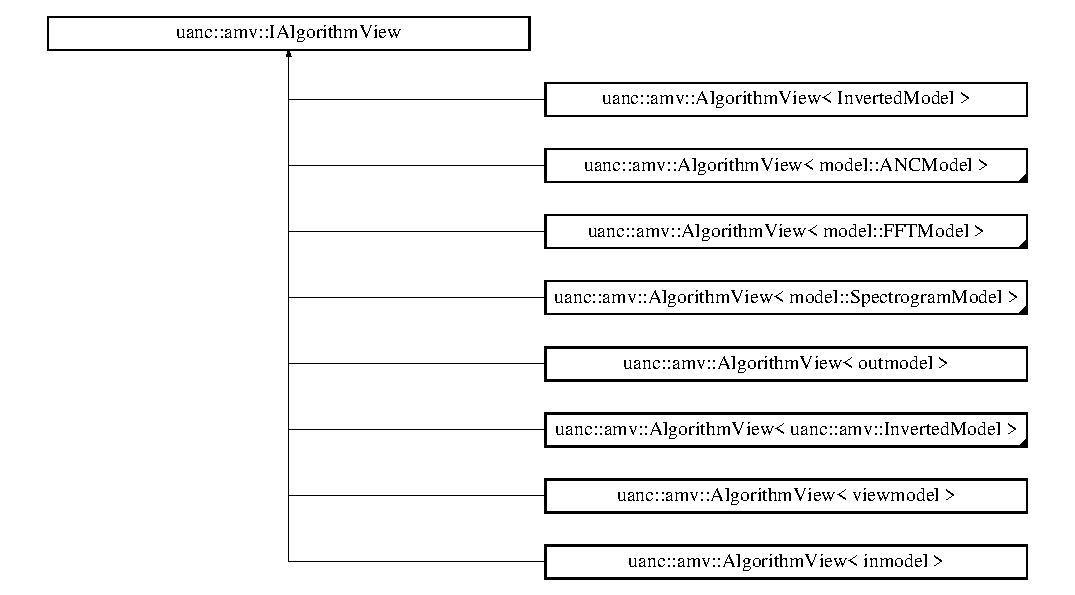
\includegraphics[height=7.544909cm]{classuanc_1_1amv_1_1_i_algorithm_view}
\end{center}
\end{figure}
\subsection*{Public Member Functions}
\begin{DoxyCompactItemize}
\item 
Q\+Widget $\ast$ \hyperlink{classuanc_1_1amv_1_1_i_algorithm_view_ad477f4e62bb8c2ae78fd010cba1628cb}{get\+Widget} ()
\begin{DoxyCompactList}\small\item\em Gets the complete widget. \end{DoxyCompactList}\item 
virtual Q\+Widget $\ast$ \hyperlink{classuanc_1_1amv_1_1_i_algorithm_view_ab9d06a0b43db57244868f10dae8e09e5}{produce\+Widget} ()=0
\begin{DoxyCompactList}\small\item\em Produces the widget. \end{DoxyCompactList}\end{DoxyCompactItemize}


\subsection{Detailed Description}
The general interface for every view. 

This interface has to implemented by any view, which should be used seamlesly in the main application. 

\subsection{Member Function Documentation}
\index{uanc\+::amv\+::\+I\+Algorithm\+View@{uanc\+::amv\+::\+I\+Algorithm\+View}!get\+Widget@{get\+Widget}}
\index{get\+Widget@{get\+Widget}!uanc\+::amv\+::\+I\+Algorithm\+View@{uanc\+::amv\+::\+I\+Algorithm\+View}}
\subsubsection[{\texorpdfstring{get\+Widget()}{getWidget()}}]{\setlength{\rightskip}{0pt plus 5cm}Q\+Widget$\ast$ uanc\+::amv\+::\+I\+Algorithm\+View\+::get\+Widget (
\begin{DoxyParamCaption}
{}
\end{DoxyParamCaption}
)\hspace{0.3cm}{\ttfamily [inline]}}\hypertarget{classuanc_1_1amv_1_1_i_algorithm_view_ad477f4e62bb8c2ae78fd010cba1628cb}{}\label{classuanc_1_1amv_1_1_i_algorithm_view_ad477f4e62bb8c2ae78fd010cba1628cb}


Gets the complete widget. 

This function is used to retrieve the widget from the view. It gets used for integration the main application

\begin{DoxyReturn}{Returns}
The created widget. 
\end{DoxyReturn}
\index{uanc\+::amv\+::\+I\+Algorithm\+View@{uanc\+::amv\+::\+I\+Algorithm\+View}!produce\+Widget@{produce\+Widget}}
\index{produce\+Widget@{produce\+Widget}!uanc\+::amv\+::\+I\+Algorithm\+View@{uanc\+::amv\+::\+I\+Algorithm\+View}}
\subsubsection[{\texorpdfstring{produce\+Widget()=0}{produceWidget()=0}}]{\setlength{\rightskip}{0pt plus 5cm}virtual Q\+Widget$\ast$ uanc\+::amv\+::\+I\+Algorithm\+View\+::produce\+Widget (
\begin{DoxyParamCaption}
{}
\end{DoxyParamCaption}
)\hspace{0.3cm}{\ttfamily [pure virtual]}}\hypertarget{classuanc_1_1amv_1_1_i_algorithm_view_ab9d06a0b43db57244868f10dae8e09e5}{}\label{classuanc_1_1amv_1_1_i_algorithm_view_ab9d06a0b43db57244868f10dae8e09e5}


Produces the widget. 

This function is used to produce the widget from the view. It gets used for integration the main application

\begin{DoxyReturn}{Returns}
The created widget. 
\end{DoxyReturn}


Implemented in \hyperlink{classuanc_1_1amv_1_1signal_1_1view_1_1_f_f_t_view_a774599a51059f878472cf72e2ce4b2b2}{uanc\+::amv\+::signal\+::view\+::\+F\+F\+T\+View}, \hyperlink{classuanc_1_1amv_1_1anc_1_1view_1_1_p_m_view_a4f4d6f52427201d7dcd671c7932824ad}{uanc\+::amv\+::anc\+::view\+::\+P\+M\+View}, \hyperlink{classuanc_1_1amv_1_1anc_1_1view_1_1_a_n_c_view_ab8ad6046c26c2eae15edc82fdbae9aa1}{uanc\+::amv\+::anc\+::view\+::\+A\+N\+C\+View}, \hyperlink{classuanc_1_1amv_1_1signal_1_1view_1_1_signal_view_a8b42dd84baf3c0730640ddb87db69735}{uanc\+::amv\+::signal\+::view\+::\+Signal\+View}, and \hyperlink{classuanc_1_1amv_1_1signal_1_1view_1_1_heat_view_a93ac20354fa17ab67e368e324f240c9a}{uanc\+::amv\+::signal\+::view\+::\+Heat\+View}.



The documentation for this class was generated from the following file\+:\begin{DoxyCompactItemize}
\item 
/home/kurt/\+Documents/\+Studium/\+Bachelor\+\_\+\+Praktikum/\+U\+A\+N\+C/\+Code/\+U\+A\+N\+C/amv/\hyperlink{_i_algorithm_view_8h}{I\+Algorithm\+View.\+h}\end{DoxyCompactItemize}

\hypertarget{classuanc_1_1amv_1_1signal_1_1algorithm_1_1_identity_transformation_algorithm}{}\section{uanc\+:\+:amv\+:\+:signal\+:\+:algorithm\+:\+:Identity\+Transformation\+Algorithm Class Reference}
\label{classuanc_1_1amv_1_1signal_1_1algorithm_1_1_identity_transformation_algorithm}\index{uanc\+::amv\+::signal\+::algorithm\+::\+Identity\+Transformation\+Algorithm@{uanc\+::amv\+::signal\+::algorithm\+::\+Identity\+Transformation\+Algorithm}}


Identity transformation.  




{\ttfamily \#include $<$Identity\+Transformation\+Algorithm.\+h$>$}

Inheritance diagram for uanc\+:\+:amv\+:\+:signal\+:\+:algorithm\+:\+:Identity\+Transformation\+Algorithm\+:\begin{figure}[H]
\begin{center}
\leavevmode
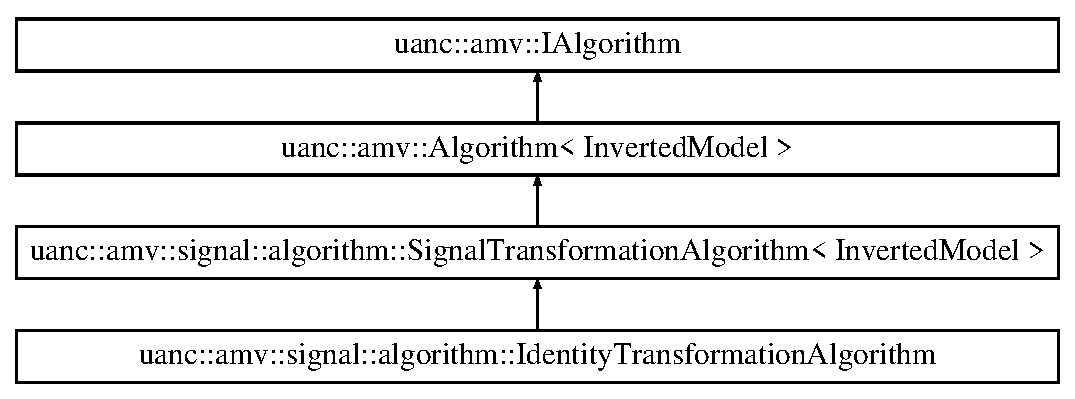
\includegraphics[height=4.000000cm]{classuanc_1_1amv_1_1signal_1_1algorithm_1_1_identity_transformation_algorithm}
\end{center}
\end{figure}
\subsection*{Public Member Functions}
\begin{DoxyCompactItemize}
\item 
std\+::string \hyperlink{classuanc_1_1amv_1_1signal_1_1algorithm_1_1_identity_transformation_algorithm_ad79e871df8798749358bd3f64cd6a4f1}{get\+Name} () final
\begin{DoxyCompactList}\small\item\em Returns the name of the transformed data representation. \end{DoxyCompactList}\item 
void \hyperlink{classuanc_1_1amv_1_1signal_1_1algorithm_1_1_identity_transformation_algorithm_aac5f7f10ab44d7f8625eb5dbb72e5c44}{transform} (std\+::shared\+\_\+ptr$<$ \hyperlink{classuanc_1_1amv_1_1_inverted_model}{uanc\+::amv\+::\+Inverted\+Model} $>$ in) final
\begin{DoxyCompactList}\small\item\em Simply saves the input signal to the output. \end{DoxyCompactList}\item 
\hyperlink{classuanc_1_1amv_1_1_algorithm}{Algorithm} $\ast$ \hyperlink{classuanc_1_1amv_1_1signal_1_1algorithm_1_1_identity_transformation_algorithm_a863e785131c7e4f7d41d403a7fb4526d}{clone} () final
\begin{DoxyCompactList}\small\item\em Clones the current instance. \end{DoxyCompactList}\end{DoxyCompactItemize}
\subsection*{Protected Member Functions}
\begin{DoxyCompactItemize}
\item 
\hyperlink{classuanc_1_1amv_1_1_algorithm_view}{Algorithm\+View}$<$ \hyperlink{classuanc_1_1amv_1_1_inverted_model}{Inverted\+Model} $>$ $\ast$ \hyperlink{classuanc_1_1amv_1_1signal_1_1algorithm_1_1_identity_transformation_algorithm_a76e6380fcbcef86de4b5aa1fd7f4b77d}{construct\+View} () final
\begin{DoxyCompactList}\small\item\em Constructs a view, which can handle an A\+N\+C\+Model. \end{DoxyCompactList}\end{DoxyCompactItemize}


\subsection{Detailed Description}
Identity transformation. 

This transformation basically outputs the same signal which was set as an input. This is neccessary for a good integration inside of the application, because we don\textquotesingle{}t want to differntiate versus direct data or transformed data views. 

\subsection{Member Function Documentation}
\index{uanc\+::amv\+::signal\+::algorithm\+::\+Identity\+Transformation\+Algorithm@{uanc\+::amv\+::signal\+::algorithm\+::\+Identity\+Transformation\+Algorithm}!clone@{clone}}
\index{clone@{clone}!uanc\+::amv\+::signal\+::algorithm\+::\+Identity\+Transformation\+Algorithm@{uanc\+::amv\+::signal\+::algorithm\+::\+Identity\+Transformation\+Algorithm}}
\subsubsection[{\texorpdfstring{clone() final}{clone() final}}]{\setlength{\rightskip}{0pt plus 5cm}{\bf Algorithm}$\ast$ uanc\+::amv\+::signal\+::algorithm\+::\+Identity\+Transformation\+Algorithm\+::clone (
\begin{DoxyParamCaption}
{}
\end{DoxyParamCaption}
)\hspace{0.3cm}{\ttfamily [inline]}, {\ttfamily [final]}, {\ttfamily [virtual]}}\hypertarget{classuanc_1_1amv_1_1signal_1_1algorithm_1_1_identity_transformation_algorithm_a863e785131c7e4f7d41d403a7fb4526d}{}\label{classuanc_1_1amv_1_1signal_1_1algorithm_1_1_identity_transformation_algorithm_a863e785131c7e4f7d41d403a7fb4526d}


Clones the current instance. 

This is basically the prototype pattern. It gets used to create an copy of the current \hyperlink{classuanc_1_1amv_1_1signal_1_1algorithm_1_1_identity_transformation_algorithm}{Identity\+Transformation\+Algorithm}. To do so it simply creates a new instance.

\begin{DoxyReturn}{Returns}
The cloned algorithm. 
\end{DoxyReturn}


Implements \hyperlink{classuanc_1_1amv_1_1_i_algorithm_af6fcbfa35f460363c2cc7e6134af8dc7}{uanc\+::amv\+::\+I\+Algorithm}.

\index{uanc\+::amv\+::signal\+::algorithm\+::\+Identity\+Transformation\+Algorithm@{uanc\+::amv\+::signal\+::algorithm\+::\+Identity\+Transformation\+Algorithm}!construct\+View@{construct\+View}}
\index{construct\+View@{construct\+View}!uanc\+::amv\+::signal\+::algorithm\+::\+Identity\+Transformation\+Algorithm@{uanc\+::amv\+::signal\+::algorithm\+::\+Identity\+Transformation\+Algorithm}}
\subsubsection[{\texorpdfstring{construct\+View() final}{constructView() final}}]{\setlength{\rightskip}{0pt plus 5cm}{\bf Algorithm\+View}$<${\bf Inverted\+Model}$>$$\ast$ uanc\+::amv\+::signal\+::algorithm\+::\+Identity\+Transformation\+Algorithm\+::construct\+View (
\begin{DoxyParamCaption}
{}
\end{DoxyParamCaption}
)\hspace{0.3cm}{\ttfamily [inline]}, {\ttfamily [final]}, {\ttfamily [protected]}, {\ttfamily [virtual]}}\hypertarget{classuanc_1_1amv_1_1signal_1_1algorithm_1_1_identity_transformation_algorithm_a76e6380fcbcef86de4b5aa1fd7f4b77d}{}\label{classuanc_1_1amv_1_1signal_1_1algorithm_1_1_identity_transformation_algorithm_a76e6380fcbcef86de4b5aa1fd7f4b77d}


Constructs a view, which can handle an A\+N\+C\+Model. 

This view basically display the standard information of the algorithm.

\begin{DoxyReturn}{Returns}
The created A\+N\+C\+View. 
\end{DoxyReturn}


Implements \hyperlink{classuanc_1_1amv_1_1_algorithm_af5561072283ed19634893263c95a4b6e}{uanc\+::amv\+::\+Algorithm$<$ Inverted\+Model $>$}.

\index{uanc\+::amv\+::signal\+::algorithm\+::\+Identity\+Transformation\+Algorithm@{uanc\+::amv\+::signal\+::algorithm\+::\+Identity\+Transformation\+Algorithm}!get\+Name@{get\+Name}}
\index{get\+Name@{get\+Name}!uanc\+::amv\+::signal\+::algorithm\+::\+Identity\+Transformation\+Algorithm@{uanc\+::amv\+::signal\+::algorithm\+::\+Identity\+Transformation\+Algorithm}}
\subsubsection[{\texorpdfstring{get\+Name() final}{getName() final}}]{\setlength{\rightskip}{0pt plus 5cm}std\+::string uanc\+::amv\+::signal\+::algorithm\+::\+Identity\+Transformation\+Algorithm\+::get\+Name (
\begin{DoxyParamCaption}
{}
\end{DoxyParamCaption}
)\hspace{0.3cm}{\ttfamily [inline]}, {\ttfamily [final]}, {\ttfamily [virtual]}}\hypertarget{classuanc_1_1amv_1_1signal_1_1algorithm_1_1_identity_transformation_algorithm_ad79e871df8798749358bd3f64cd6a4f1}{}\label{classuanc_1_1amv_1_1signal_1_1algorithm_1_1_identity_transformation_algorithm_ad79e871df8798749358bd3f64cd6a4f1}


Returns the name of the transformed data representation. 

Simply passes back the name of the data transformation

\begin{DoxyReturn}{Returns}
Name of the data transformation 
\end{DoxyReturn}


Implements \hyperlink{classuanc_1_1amv_1_1_i_algorithm_a4935ab2fdacccf7df35d6fb596075edb}{uanc\+::amv\+::\+I\+Algorithm}.

\index{uanc\+::amv\+::signal\+::algorithm\+::\+Identity\+Transformation\+Algorithm@{uanc\+::amv\+::signal\+::algorithm\+::\+Identity\+Transformation\+Algorithm}!transform@{transform}}
\index{transform@{transform}!uanc\+::amv\+::signal\+::algorithm\+::\+Identity\+Transformation\+Algorithm@{uanc\+::amv\+::signal\+::algorithm\+::\+Identity\+Transformation\+Algorithm}}
\subsubsection[{\texorpdfstring{transform(std\+::shared\+\_\+ptr$<$ uanc\+::amv\+::\+Inverted\+Model $>$ in) final}{transform(std::shared_ptr< uanc::amv::InvertedModel > in) final}}]{\setlength{\rightskip}{0pt plus 5cm}void uanc\+::amv\+::signal\+::algorithm\+::\+Identity\+Transformation\+Algorithm\+::transform (
\begin{DoxyParamCaption}
\item[{std\+::shared\+\_\+ptr$<$ {\bf uanc\+::amv\+::\+Inverted\+Model} $>$}]{in}
\end{DoxyParamCaption}
)\hspace{0.3cm}{\ttfamily [inline]}, {\ttfamily [final]}, {\ttfamily [virtual]}}\hypertarget{classuanc_1_1amv_1_1signal_1_1algorithm_1_1_identity_transformation_algorithm_aac5f7f10ab44d7f8625eb5dbb72e5c44}{}\label{classuanc_1_1amv_1_1signal_1_1algorithm_1_1_identity_transformation_algorithm_aac5f7f10ab44d7f8625eb5dbb72e5c44}


Simply saves the input signal to the output. 

This method just passes back the input model signal. It is only needed for integration purposes.


\begin{DoxyParams}{Parameters}
{\em input} & The input model containing the original signal. \\
\hline
\end{DoxyParams}


Implements \hyperlink{classuanc_1_1amv_1_1signal_1_1algorithm_1_1_signal_transformation_algorithm_a40dee2d59e84244373cacc9c472514d6}{uanc\+::amv\+::signal\+::algorithm\+::\+Signal\+Transformation\+Algorithm$<$ Inverted\+Model $>$}.



The documentation for this class was generated from the following file\+:\begin{DoxyCompactItemize}
\item 
/ext/local/\+University/\+B\+P/\+Git/\+U\+A\+N\+C/\+Code/\+U\+A\+N\+C/amv/signal/algorithm/\hyperlink{_identity_transformation_algorithm_8h}{Identity\+Transformation\+Algorithm.\+h}\end{DoxyCompactItemize}

\hypertarget{classuanc_1_1gui_1_1_import_window}{}\section{uanc\+:\+:gui\+:\+:Import\+Window Class Reference}
\label{classuanc_1_1gui_1_1_import_window}\index{uanc\+::gui\+::\+Import\+Window@{uanc\+::gui\+::\+Import\+Window}}


{\ttfamily \#include $<$Import\+Window.\+h$>$}

Inheritance diagram for uanc\+:\+:gui\+:\+:Import\+Window\+:\begin{figure}[H]
\begin{center}
\leavevmode
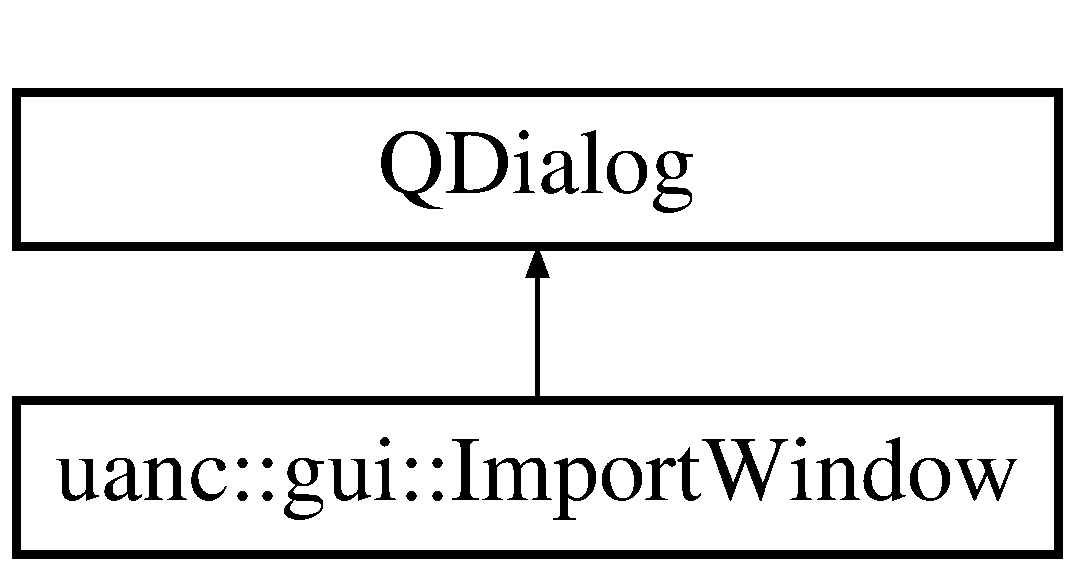
\includegraphics[height=2.000000cm]{classuanc_1_1gui_1_1_import_window}
\end{center}
\end{figure}
\subsection*{Signals}
\begin{DoxyCompactItemize}
\item 
void \hyperlink{classuanc_1_1gui_1_1_import_window_ac355137ecc8de30b572c3e1df7a16b81}{indices\+Loaded} (std\+::vector$<$ int $>$ loaded\+Indices)
\begin{DoxyCompactList}\small\item\em \+: Slot that indicates that signals have been selected and loaded successfully into the Signal\+Manager \end{DoxyCompactList}\end{DoxyCompactItemize}
\subsection*{Public Member Functions}
\begin{DoxyCompactItemize}
\item 
\hyperlink{classuanc_1_1gui_1_1_import_window_a812ba3dd89d0f90774dd5089a499a98b}{Import\+Window} (Q\+Widget $\ast$parent)
\end{DoxyCompactItemize}


\subsection{Constructor \& Destructor Documentation}
\index{uanc\+::gui\+::\+Import\+Window@{uanc\+::gui\+::\+Import\+Window}!Import\+Window@{Import\+Window}}
\index{Import\+Window@{Import\+Window}!uanc\+::gui\+::\+Import\+Window@{uanc\+::gui\+::\+Import\+Window}}
\subsubsection[{\texorpdfstring{Import\+Window(\+Q\+Widget $\ast$parent)}{ImportWindow(QWidget *parent)}}]{\setlength{\rightskip}{0pt plus 5cm}uanc\+::gui\+::\+Import\+Window\+::\+Import\+Window (
\begin{DoxyParamCaption}
\item[{Q\+Widget $\ast$}]{parent}
\end{DoxyParamCaption}
)}\hypertarget{classuanc_1_1gui_1_1_import_window_a812ba3dd89d0f90774dd5089a499a98b}{}\label{classuanc_1_1gui_1_1_import_window_a812ba3dd89d0f90774dd5089a499a98b}
The default constructor 

\subsection{Member Function Documentation}
\index{uanc\+::gui\+::\+Import\+Window@{uanc\+::gui\+::\+Import\+Window}!indices\+Loaded@{indices\+Loaded}}
\index{indices\+Loaded@{indices\+Loaded}!uanc\+::gui\+::\+Import\+Window@{uanc\+::gui\+::\+Import\+Window}}
\subsubsection[{\texorpdfstring{indices\+Loaded}{indicesLoaded}}]{\setlength{\rightskip}{0pt plus 5cm}void uanc\+::gui\+::\+Import\+Window\+::indices\+Loaded (
\begin{DoxyParamCaption}
\item[{std\+::vector$<$ int $>$}]{loaded\+Indices}
\end{DoxyParamCaption}
)\hspace{0.3cm}{\ttfamily [signal]}}\hypertarget{classuanc_1_1gui_1_1_import_window_ac355137ecc8de30b572c3e1df7a16b81}{}\label{classuanc_1_1gui_1_1_import_window_ac355137ecc8de30b572c3e1df7a16b81}


\+: Slot that indicates that signals have been selected and loaded successfully into the Signal\+Manager 



The documentation for this class was generated from the following files\+:\begin{DoxyCompactItemize}
\item 
/ext/local/\+University/\+B\+P/\+Git/\+U\+A\+N\+C/\+Code/\+U\+A\+N\+C/gui/\hyperlink{_import_window_8h}{Import\+Window.\+h}\item 
/ext/local/\+University/\+B\+P/\+Git/\+U\+A\+N\+C/\+Code/\+U\+A\+N\+C/gui/\hyperlink{_import_window_8cpp}{Import\+Window.\+cpp}\end{DoxyCompactItemize}

\hypertarget{classuanc_1_1amv_1_1anc_1_1algorithm_1_1_inverse_direct_algorithm}{}\section{uanc\+:\+:amv\+:\+:anc\+:\+:algorithm\+:\+:Inverse\+Direct\+Algorithm Class Reference}
\label{classuanc_1_1amv_1_1anc_1_1algorithm_1_1_inverse_direct_algorithm}\index{uanc\+::amv\+::anc\+::algorithm\+::\+Inverse\+Direct\+Algorithm@{uanc\+::amv\+::anc\+::algorithm\+::\+Inverse\+Direct\+Algorithm}}


Direct inversion algorithm.  




{\ttfamily \#include $<$Inverse\+Direct\+Algorithm.\+h$>$}

Inheritance diagram for uanc\+:\+:amv\+:\+:anc\+:\+:algorithm\+:\+:Inverse\+Direct\+Algorithm\+:\begin{figure}[H]
\begin{center}
\leavevmode
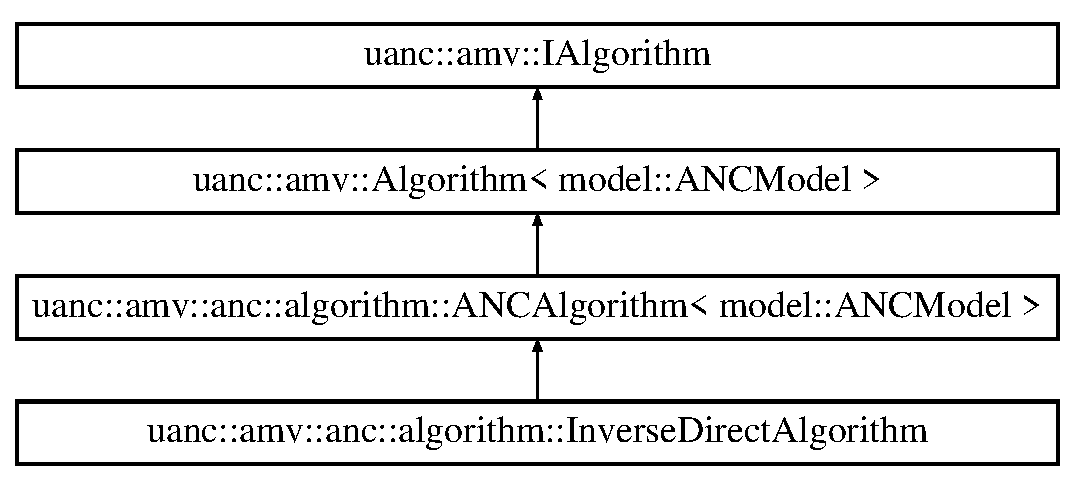
\includegraphics[height=4.000000cm]{classuanc_1_1amv_1_1anc_1_1algorithm_1_1_inverse_direct_algorithm}
\end{center}
\end{figure}
\subsection*{Public Member Functions}
\begin{DoxyCompactItemize}
\item 
std\+::string \hyperlink{classuanc_1_1amv_1_1anc_1_1algorithm_1_1_inverse_direct_algorithm_af7933bf4a0ad32c58688d8d74c6f2487}{get\+Name} () final
\begin{DoxyCompactList}\small\item\em Returns the name of the algorithm. \end{DoxyCompactList}\item 
void \hyperlink{classuanc_1_1amv_1_1anc_1_1algorithm_1_1_inverse_direct_algorithm_a4bd1bdcd128aee1f608be51660528954}{invert} (std\+::shared\+\_\+ptr$<$ \hyperlink{classuanc_1_1amv_1_1_inverted_model}{Inverted\+Model} $>$ in)
\begin{DoxyCompactList}\small\item\em Inverts the input signal. \end{DoxyCompactList}\item 
\hyperlink{classuanc_1_1amv_1_1_algorithm}{Algorithm} $\ast$ \hyperlink{classuanc_1_1amv_1_1anc_1_1algorithm_1_1_inverse_direct_algorithm_adce538c00ba00237ba29d725abaae764}{clone} () final
\begin{DoxyCompactList}\small\item\em Clones the current instance. \end{DoxyCompactList}\end{DoxyCompactItemize}
\subsection*{Protected Member Functions}
\begin{DoxyCompactItemize}
\item 
\hyperlink{classuanc_1_1amv_1_1_algorithm_view}{Algorithm\+View}$<$ \hyperlink{classuanc_1_1amv_1_1anc_1_1model_1_1_a_n_c_model}{model\+::\+A\+N\+C\+Model} $>$ $\ast$ \hyperlink{classuanc_1_1amv_1_1anc_1_1algorithm_1_1_inverse_direct_algorithm_ad470192f0ae1042f16750a9181cb61c0}{construct\+View} () final
\begin{DoxyCompactList}\small\item\em Constructs a view, which can handle an A\+N\+C\+Model. \end{DoxyCompactList}\end{DoxyCompactItemize}


\subsection{Detailed Description}
Direct inversion algorithm. 

This class represents a direct inversion algorithm. It simply multiplies every sample by -\/1 and outputs the final signal. It uses the simplest working model for \hyperlink{classuanc_1_1amv_1_1anc_1_1algorithm_1_1_a_n_c_algorithm}{A\+N\+C\+Algorithm} (A\+N\+C\+Model) 

\subsection{Member Function Documentation}
\index{uanc\+::amv\+::anc\+::algorithm\+::\+Inverse\+Direct\+Algorithm@{uanc\+::amv\+::anc\+::algorithm\+::\+Inverse\+Direct\+Algorithm}!clone@{clone}}
\index{clone@{clone}!uanc\+::amv\+::anc\+::algorithm\+::\+Inverse\+Direct\+Algorithm@{uanc\+::amv\+::anc\+::algorithm\+::\+Inverse\+Direct\+Algorithm}}
\subsubsection[{\texorpdfstring{clone() final}{clone() final}}]{\setlength{\rightskip}{0pt plus 5cm}{\bf Algorithm}$\ast$ uanc\+::amv\+::anc\+::algorithm\+::\+Inverse\+Direct\+Algorithm\+::clone (
\begin{DoxyParamCaption}
{}
\end{DoxyParamCaption}
)\hspace{0.3cm}{\ttfamily [inline]}, {\ttfamily [final]}, {\ttfamily [virtual]}}\hypertarget{classuanc_1_1amv_1_1anc_1_1algorithm_1_1_inverse_direct_algorithm_adce538c00ba00237ba29d725abaae764}{}\label{classuanc_1_1amv_1_1anc_1_1algorithm_1_1_inverse_direct_algorithm_adce538c00ba00237ba29d725abaae764}


Clones the current instance. 

This is basically the prototype pattern. It gets used to create an copy of the current \hyperlink{classuanc_1_1amv_1_1anc_1_1algorithm_1_1_inverse_direct_algorithm}{Inverse\+Direct\+Algorithm}. To do so it simply creates a new instance.

\begin{DoxyReturn}{Returns}
The cloned algorithm. 
\end{DoxyReturn}


Implements \hyperlink{classuanc_1_1amv_1_1_i_algorithm_af6fcbfa35f460363c2cc7e6134af8dc7}{uanc\+::amv\+::\+I\+Algorithm}.

\index{uanc\+::amv\+::anc\+::algorithm\+::\+Inverse\+Direct\+Algorithm@{uanc\+::amv\+::anc\+::algorithm\+::\+Inverse\+Direct\+Algorithm}!construct\+View@{construct\+View}}
\index{construct\+View@{construct\+View}!uanc\+::amv\+::anc\+::algorithm\+::\+Inverse\+Direct\+Algorithm@{uanc\+::amv\+::anc\+::algorithm\+::\+Inverse\+Direct\+Algorithm}}
\subsubsection[{\texorpdfstring{construct\+View() final}{constructView() final}}]{\setlength{\rightskip}{0pt plus 5cm}{\bf Algorithm\+View}$<${\bf model\+::\+A\+N\+C\+Model}$>$$\ast$ uanc\+::amv\+::anc\+::algorithm\+::\+Inverse\+Direct\+Algorithm\+::construct\+View (
\begin{DoxyParamCaption}
{}
\end{DoxyParamCaption}
)\hspace{0.3cm}{\ttfamily [inline]}, {\ttfamily [final]}, {\ttfamily [protected]}, {\ttfamily [virtual]}}\hypertarget{classuanc_1_1amv_1_1anc_1_1algorithm_1_1_inverse_direct_algorithm_ad470192f0ae1042f16750a9181cb61c0}{}\label{classuanc_1_1amv_1_1anc_1_1algorithm_1_1_inverse_direct_algorithm_ad470192f0ae1042f16750a9181cb61c0}


Constructs a view, which can handle an A\+N\+C\+Model. 

This view basically display the standard information of the algorithm.

\begin{DoxyReturn}{Returns}
The created A\+N\+C\+View. 
\end{DoxyReturn}


Implements \hyperlink{classuanc_1_1amv_1_1_algorithm_af5561072283ed19634893263c95a4b6e}{uanc\+::amv\+::\+Algorithm$<$ model\+::\+A\+N\+C\+Model $>$}.

\index{uanc\+::amv\+::anc\+::algorithm\+::\+Inverse\+Direct\+Algorithm@{uanc\+::amv\+::anc\+::algorithm\+::\+Inverse\+Direct\+Algorithm}!get\+Name@{get\+Name}}
\index{get\+Name@{get\+Name}!uanc\+::amv\+::anc\+::algorithm\+::\+Inverse\+Direct\+Algorithm@{uanc\+::amv\+::anc\+::algorithm\+::\+Inverse\+Direct\+Algorithm}}
\subsubsection[{\texorpdfstring{get\+Name() final}{getName() final}}]{\setlength{\rightskip}{0pt plus 5cm}std\+::string uanc\+::amv\+::anc\+::algorithm\+::\+Inverse\+Direct\+Algorithm\+::get\+Name (
\begin{DoxyParamCaption}
{}
\end{DoxyParamCaption}
)\hspace{0.3cm}{\ttfamily [inline]}, {\ttfamily [final]}, {\ttfamily [virtual]}}\hypertarget{classuanc_1_1amv_1_1anc_1_1algorithm_1_1_inverse_direct_algorithm_af7933bf4a0ad32c58688d8d74c6f2487}{}\label{classuanc_1_1amv_1_1anc_1_1algorithm_1_1_inverse_direct_algorithm_af7933bf4a0ad32c58688d8d74c6f2487}


Returns the name of the algorithm. 

Simply passes back the name of the algorithm.

\begin{DoxyReturn}{Returns}
Name of the algorithm 
\end{DoxyReturn}


Implements \hyperlink{classuanc_1_1amv_1_1_i_algorithm_a4935ab2fdacccf7df35d6fb596075edb}{uanc\+::amv\+::\+I\+Algorithm}.

\index{uanc\+::amv\+::anc\+::algorithm\+::\+Inverse\+Direct\+Algorithm@{uanc\+::amv\+::anc\+::algorithm\+::\+Inverse\+Direct\+Algorithm}!invert@{invert}}
\index{invert@{invert}!uanc\+::amv\+::anc\+::algorithm\+::\+Inverse\+Direct\+Algorithm@{uanc\+::amv\+::anc\+::algorithm\+::\+Inverse\+Direct\+Algorithm}}
\subsubsection[{\texorpdfstring{invert(std\+::shared\+\_\+ptr$<$ Inverted\+Model $>$ in)}{invert(std::shared_ptr< InvertedModel > in)}}]{\setlength{\rightskip}{0pt plus 5cm}void uanc\+::amv\+::anc\+::algorithm\+::\+Inverse\+Direct\+Algorithm\+::invert (
\begin{DoxyParamCaption}
\item[{std\+::shared\+\_\+ptr$<$ {\bf Inverted\+Model} $>$}]{in}
\end{DoxyParamCaption}
)\hspace{0.3cm}{\ttfamily [inline]}, {\ttfamily [virtual]}}\hypertarget{classuanc_1_1amv_1_1anc_1_1algorithm_1_1_inverse_direct_algorithm_a4bd1bdcd128aee1f608be51660528954}{}\label{classuanc_1_1amv_1_1anc_1_1algorithm_1_1_inverse_direct_algorithm_a4bd1bdcd128aee1f608be51660528954}


Inverts the input signal. 

This is actually the heart of an A\+NC algorithm inside of this application. It takes an input model and processes it. Besides it should save its data inside the model using \hyperlink{classuanc_1_1amv_1_1anc_1_1algorithm_1_1_a_n_c_algorithm_a12ce80f6746cbb440cf771fc6878f7cf}{get\+Model()}.


\begin{DoxyParams}{Parameters}
{\em input} & The input model containing the original signal. \\
\hline
\end{DoxyParams}


Implements \hyperlink{classuanc_1_1amv_1_1anc_1_1algorithm_1_1_a_n_c_algorithm_abfdc7f14f7e41e408ee08037a839760d}{uanc\+::amv\+::anc\+::algorithm\+::\+A\+N\+C\+Algorithm$<$ model\+::\+A\+N\+C\+Model $>$}.



The documentation for this class was generated from the following file\+:\begin{DoxyCompactItemize}
\item 
/home/kurt/\+Documents/\+Studium/\+Bachelor\+\_\+\+Praktikum/\+U\+A\+N\+C/\+Code/\+U\+A\+N\+C/amv/anc/algorithm/\hyperlink{_inverse_direct_algorithm_8h}{Inverse\+Direct\+Algorithm.\+h}\end{DoxyCompactItemize}

\hypertarget{classuanc_1_1amv_1_1anc_1_1algorithm_1_1_inverse_f_f_t_algorithm}{}\section{uanc\+:\+:amv\+:\+:anc\+:\+:algorithm\+:\+:Inverse\+F\+F\+T\+Algorithm Class Reference}
\label{classuanc_1_1amv_1_1anc_1_1algorithm_1_1_inverse_f_f_t_algorithm}\index{uanc\+::amv\+::anc\+::algorithm\+::\+Inverse\+F\+F\+T\+Algorithm@{uanc\+::amv\+::anc\+::algorithm\+::\+Inverse\+F\+F\+T\+Algorithm}}


F\+FT inversion algorithm.  




{\ttfamily \#include $<$Inverse\+F\+F\+T\+Algorithm.\+h$>$}

Inheritance diagram for uanc\+:\+:amv\+:\+:anc\+:\+:algorithm\+:\+:Inverse\+F\+F\+T\+Algorithm\+:\begin{figure}[H]
\begin{center}
\leavevmode
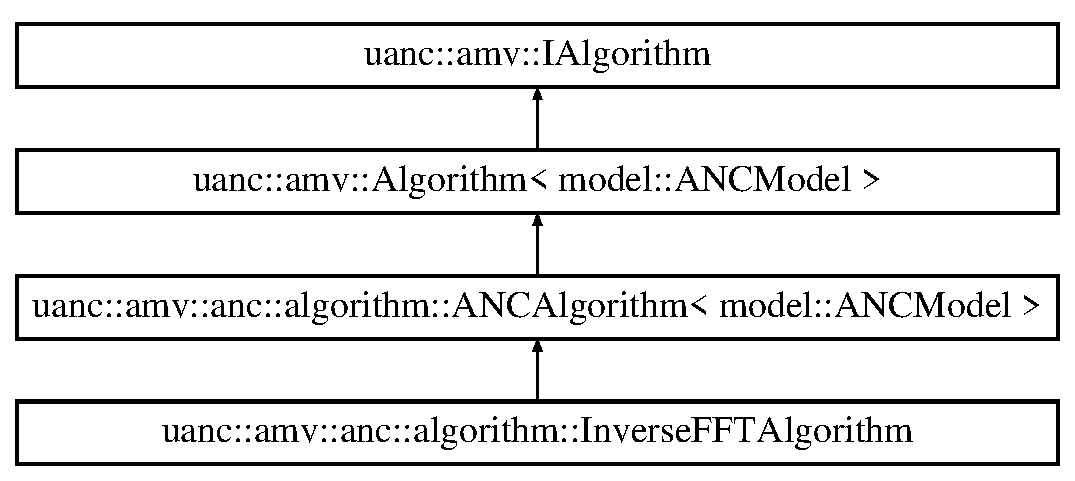
\includegraphics[height=4.000000cm]{classuanc_1_1amv_1_1anc_1_1algorithm_1_1_inverse_f_f_t_algorithm}
\end{center}
\end{figure}
\subsection*{Public Member Functions}
\begin{DoxyCompactItemize}
\item 
std\+::string \hyperlink{classuanc_1_1amv_1_1anc_1_1algorithm_1_1_inverse_f_f_t_algorithm_a7f412ced258f067f47e865608de16cd6}{get\+Name} () final
\begin{DoxyCompactList}\small\item\em Returns the name of the algorithm. \end{DoxyCompactList}\item 
void \hyperlink{classuanc_1_1amv_1_1anc_1_1algorithm_1_1_inverse_f_f_t_algorithm_a75d38b5ce03bca80a856dfa257f590a4}{invert} (std\+::shared\+\_\+ptr$<$ \hyperlink{classuanc_1_1amv_1_1_inverted_model}{Inverted\+Model} $>$ data) final
\begin{DoxyCompactList}\small\item\em Inverts the input signal. \end{DoxyCompactList}\item 
\hyperlink{classuanc_1_1amv_1_1_algorithm}{Algorithm} $\ast$ \hyperlink{classuanc_1_1amv_1_1anc_1_1algorithm_1_1_inverse_f_f_t_algorithm_abb8ee8a2ba58c14cf2a138657f3cc211}{clone} () final
\begin{DoxyCompactList}\small\item\em Clones the current instance. \end{DoxyCompactList}\end{DoxyCompactItemize}
\subsection*{Protected Member Functions}
\begin{DoxyCompactItemize}
\item 
\hyperlink{classuanc_1_1amv_1_1_algorithm_view}{Algorithm\+View}$<$ \hyperlink{classuanc_1_1amv_1_1anc_1_1model_1_1_a_n_c_model}{model\+::\+A\+N\+C\+Model} $>$ $\ast$ \hyperlink{classuanc_1_1amv_1_1anc_1_1algorithm_1_1_inverse_f_f_t_algorithm_ae2e62b5fc9ef0a7173d86078d5133009}{construct\+View} () override
\begin{DoxyCompactList}\small\item\em Constructs a view, which can handle an A\+N\+C\+Model. \end{DoxyCompactList}\end{DoxyCompactItemize}


\subsection{Detailed Description}
F\+FT inversion algorithm. 

This class represents a fft inversion algorithm. It simply transformes the data in the fourier room, inverts it and passed it back. 

\subsection{Member Function Documentation}
\index{uanc\+::amv\+::anc\+::algorithm\+::\+Inverse\+F\+F\+T\+Algorithm@{uanc\+::amv\+::anc\+::algorithm\+::\+Inverse\+F\+F\+T\+Algorithm}!clone@{clone}}
\index{clone@{clone}!uanc\+::amv\+::anc\+::algorithm\+::\+Inverse\+F\+F\+T\+Algorithm@{uanc\+::amv\+::anc\+::algorithm\+::\+Inverse\+F\+F\+T\+Algorithm}}
\subsubsection[{\texorpdfstring{clone() final}{clone() final}}]{\setlength{\rightskip}{0pt plus 5cm}{\bf Algorithm}$\ast$ uanc\+::amv\+::anc\+::algorithm\+::\+Inverse\+F\+F\+T\+Algorithm\+::clone (
\begin{DoxyParamCaption}
{}
\end{DoxyParamCaption}
)\hspace{0.3cm}{\ttfamily [inline]}, {\ttfamily [final]}, {\ttfamily [virtual]}}\hypertarget{classuanc_1_1amv_1_1anc_1_1algorithm_1_1_inverse_f_f_t_algorithm_abb8ee8a2ba58c14cf2a138657f3cc211}{}\label{classuanc_1_1amv_1_1anc_1_1algorithm_1_1_inverse_f_f_t_algorithm_abb8ee8a2ba58c14cf2a138657f3cc211}


Clones the current instance. 

This is basically the prototype pattern. It gets used to create an copy of the current \hyperlink{classuanc_1_1amv_1_1anc_1_1algorithm_1_1_inverse_direct_algorithm}{Inverse\+Direct\+Algorithm}. To do so it simply creates a new instance.

\begin{DoxyReturn}{Returns}
The cloned algorithm. 
\end{DoxyReturn}


Implements \hyperlink{classuanc_1_1amv_1_1_i_algorithm_af6fcbfa35f460363c2cc7e6134af8dc7}{uanc\+::amv\+::\+I\+Algorithm}.

\index{uanc\+::amv\+::anc\+::algorithm\+::\+Inverse\+F\+F\+T\+Algorithm@{uanc\+::amv\+::anc\+::algorithm\+::\+Inverse\+F\+F\+T\+Algorithm}!construct\+View@{construct\+View}}
\index{construct\+View@{construct\+View}!uanc\+::amv\+::anc\+::algorithm\+::\+Inverse\+F\+F\+T\+Algorithm@{uanc\+::amv\+::anc\+::algorithm\+::\+Inverse\+F\+F\+T\+Algorithm}}
\subsubsection[{\texorpdfstring{construct\+View() override}{constructView() override}}]{\setlength{\rightskip}{0pt plus 5cm}{\bf Algorithm\+View}$<${\bf model\+::\+A\+N\+C\+Model}$>$$\ast$ uanc\+::amv\+::anc\+::algorithm\+::\+Inverse\+F\+F\+T\+Algorithm\+::construct\+View (
\begin{DoxyParamCaption}
{}
\end{DoxyParamCaption}
)\hspace{0.3cm}{\ttfamily [inline]}, {\ttfamily [override]}, {\ttfamily [protected]}, {\ttfamily [virtual]}}\hypertarget{classuanc_1_1amv_1_1anc_1_1algorithm_1_1_inverse_f_f_t_algorithm_ae2e62b5fc9ef0a7173d86078d5133009}{}\label{classuanc_1_1amv_1_1anc_1_1algorithm_1_1_inverse_f_f_t_algorithm_ae2e62b5fc9ef0a7173d86078d5133009}


Constructs a view, which can handle an A\+N\+C\+Model. 

This view basically display the standard information of the algorithm.

\begin{DoxyReturn}{Returns}
The created A\+N\+C\+View. 
\end{DoxyReturn}


Implements \hyperlink{classuanc_1_1amv_1_1_algorithm_af5561072283ed19634893263c95a4b6e}{uanc\+::amv\+::\+Algorithm$<$ model\+::\+A\+N\+C\+Model $>$}.

\index{uanc\+::amv\+::anc\+::algorithm\+::\+Inverse\+F\+F\+T\+Algorithm@{uanc\+::amv\+::anc\+::algorithm\+::\+Inverse\+F\+F\+T\+Algorithm}!get\+Name@{get\+Name}}
\index{get\+Name@{get\+Name}!uanc\+::amv\+::anc\+::algorithm\+::\+Inverse\+F\+F\+T\+Algorithm@{uanc\+::amv\+::anc\+::algorithm\+::\+Inverse\+F\+F\+T\+Algorithm}}
\subsubsection[{\texorpdfstring{get\+Name() final}{getName() final}}]{\setlength{\rightskip}{0pt plus 5cm}std\+::string uanc\+::amv\+::anc\+::algorithm\+::\+Inverse\+F\+F\+T\+Algorithm\+::get\+Name (
\begin{DoxyParamCaption}
{}
\end{DoxyParamCaption}
)\hspace{0.3cm}{\ttfamily [inline]}, {\ttfamily [final]}, {\ttfamily [virtual]}}\hypertarget{classuanc_1_1amv_1_1anc_1_1algorithm_1_1_inverse_f_f_t_algorithm_a7f412ced258f067f47e865608de16cd6}{}\label{classuanc_1_1amv_1_1anc_1_1algorithm_1_1_inverse_f_f_t_algorithm_a7f412ced258f067f47e865608de16cd6}


Returns the name of the algorithm. 

Simply passes back the name of the algorithm.

\begin{DoxyReturn}{Returns}
Name of the algorithm 
\end{DoxyReturn}


Implements \hyperlink{classuanc_1_1amv_1_1_i_algorithm_a4935ab2fdacccf7df35d6fb596075edb}{uanc\+::amv\+::\+I\+Algorithm}.

\index{uanc\+::amv\+::anc\+::algorithm\+::\+Inverse\+F\+F\+T\+Algorithm@{uanc\+::amv\+::anc\+::algorithm\+::\+Inverse\+F\+F\+T\+Algorithm}!invert@{invert}}
\index{invert@{invert}!uanc\+::amv\+::anc\+::algorithm\+::\+Inverse\+F\+F\+T\+Algorithm@{uanc\+::amv\+::anc\+::algorithm\+::\+Inverse\+F\+F\+T\+Algorithm}}
\subsubsection[{\texorpdfstring{invert(std\+::shared\+\_\+ptr$<$ Inverted\+Model $>$ data) final}{invert(std::shared_ptr< InvertedModel > data) final}}]{\setlength{\rightskip}{0pt plus 5cm}void uanc\+::amv\+::anc\+::algorithm\+::\+Inverse\+F\+F\+T\+Algorithm\+::invert (
\begin{DoxyParamCaption}
\item[{std\+::shared\+\_\+ptr$<$ {\bf Inverted\+Model} $>$}]{data}
\end{DoxyParamCaption}
)\hspace{0.3cm}{\ttfamily [inline]}, {\ttfamily [final]}, {\ttfamily [virtual]}}\hypertarget{classuanc_1_1amv_1_1anc_1_1algorithm_1_1_inverse_f_f_t_algorithm_a75d38b5ce03bca80a856dfa257f590a4}{}\label{classuanc_1_1amv_1_1anc_1_1algorithm_1_1_inverse_f_f_t_algorithm_a75d38b5ce03bca80a856dfa257f590a4}


Inverts the input signal. 

This is actually the heart of an A\+NC algorithm inside of this application. It takes an input model and processes it. Besides it should save its data inside the model using \hyperlink{classuanc_1_1amv_1_1anc_1_1algorithm_1_1_a_n_c_algorithm_a12ce80f6746cbb440cf771fc6878f7cf}{get\+Model()}.


\begin{DoxyParams}{Parameters}
{\em input} & The input model containing the original signal. \\
\hline
\end{DoxyParams}


Implements \hyperlink{classuanc_1_1amv_1_1anc_1_1algorithm_1_1_a_n_c_algorithm_abfdc7f14f7e41e408ee08037a839760d}{uanc\+::amv\+::anc\+::algorithm\+::\+A\+N\+C\+Algorithm$<$ model\+::\+A\+N\+C\+Model $>$}.



The documentation for this class was generated from the following file\+:\begin{DoxyCompactItemize}
\item 
/home/kurt/\+Documents/\+Studium/\+Bachelor\+\_\+\+Praktikum/\+U\+A\+N\+C/\+Code/\+U\+A\+N\+C/amv/anc/algorithm/\hyperlink{_inverse_f_f_t_algorithm_8h}{Inverse\+F\+F\+T\+Algorithm.\+h}\end{DoxyCompactItemize}

\hypertarget{classuanc_1_1amv_1_1_inverted_model}{}\section{uanc\+:\+:amv\+:\+:Inverted\+Model Class Reference}
\label{classuanc_1_1amv_1_1_inverted_model}\index{uanc\+::amv\+::\+Inverted\+Model@{uanc\+::amv\+::\+Inverted\+Model}}


This is an \hyperlink{classuanc_1_1amv_1_1_inverted_model}{Inverted\+Model}.  




{\ttfamily \#include $<$Inverted\+Model.\+h$>$}

Inheritance diagram for uanc\+:\+:amv\+:\+:Inverted\+Model\+:\begin{figure}[H]
\begin{center}
\leavevmode
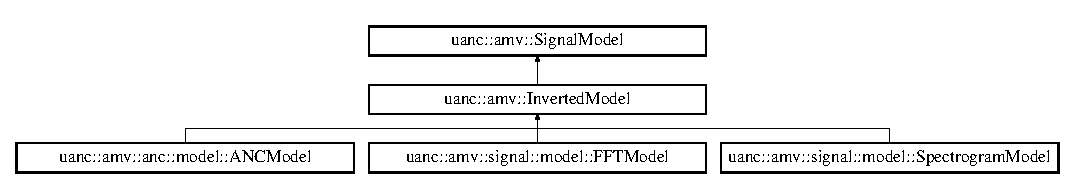
\includegraphics[height=2.089552cm]{classuanc_1_1amv_1_1_inverted_model}
\end{center}
\end{figure}
\subsection*{Public Attributes}
\begin{DoxyCompactItemize}
\item 
std\+::shared\+\_\+ptr$<$ \hyperlink{classuanc_1_1amv_1_1_signal_model}{Signal\+Model} $>$ \hyperlink{classuanc_1_1amv_1_1_inverted_model_a739f026c7b9bd28add6c8b04c4976844}{inverted} = N\+U\+LL
\begin{DoxyCompactList}\small\item\em Holds the inverted signal. \end{DoxyCompactList}\end{DoxyCompactItemize}


\subsection{Detailed Description}
This is an \hyperlink{classuanc_1_1amv_1_1_inverted_model}{Inverted\+Model}. 

This model gets derived from the \hyperlink{classuanc_1_1amv_1_1_signal_model}{Signal\+Model}. It adds a field containing the inverted signal to the original signal in \hyperlink{classuanc_1_1amv_1_1_signal_model}{Signal\+Model}. 

\subsection{Member Data Documentation}
\index{uanc\+::amv\+::\+Inverted\+Model@{uanc\+::amv\+::\+Inverted\+Model}!inverted@{inverted}}
\index{inverted@{inverted}!uanc\+::amv\+::\+Inverted\+Model@{uanc\+::amv\+::\+Inverted\+Model}}
\subsubsection[{\texorpdfstring{inverted}{inverted}}]{\setlength{\rightskip}{0pt plus 5cm}std\+::shared\+\_\+ptr$<${\bf Signal\+Model}$>$ uanc\+::amv\+::\+Inverted\+Model\+::inverted = N\+U\+LL}\hypertarget{classuanc_1_1amv_1_1_inverted_model_a739f026c7b9bd28add6c8b04c4976844}{}\label{classuanc_1_1amv_1_1_inverted_model_a739f026c7b9bd28add6c8b04c4976844}


Holds the inverted signal. 

This field gets used, to save the inverted signal, in addition to the original signal, which is placed in the parent class \hyperlink{classuanc_1_1amv_1_1_signal_model}{Signal\+Model}. 

The documentation for this class was generated from the following file\+:\begin{DoxyCompactItemize}
\item 
/home/kurt/\+Documents/\+Studium/\+Bachelor\+\_\+\+Praktikum/\+U\+A\+N\+C/\+Code/\+U\+A\+N\+C/amv/\hyperlink{_inverted_model_8h}{Inverted\+Model.\+h}\end{DoxyCompactItemize}

\hypertarget{classuanc_1_1amv_1_1anc_1_1algorithm_1_1_linear_extrapolation}{}\section{uanc\+:\+:amv\+:\+:anc\+:\+:algorithm\+:\+:Linear\+Extrapolation Class Reference}
\label{classuanc_1_1amv_1_1anc_1_1algorithm_1_1_linear_extrapolation}\index{uanc\+::amv\+::anc\+::algorithm\+::\+Linear\+Extrapolation@{uanc\+::amv\+::anc\+::algorithm\+::\+Linear\+Extrapolation}}


{\ttfamily \#include $<$Linear\+Extrapolation.\+h$>$}

Inheritance diagram for uanc\+:\+:amv\+:\+:anc\+:\+:algorithm\+:\+:Linear\+Extrapolation\+:\begin{figure}[H]
\begin{center}
\leavevmode
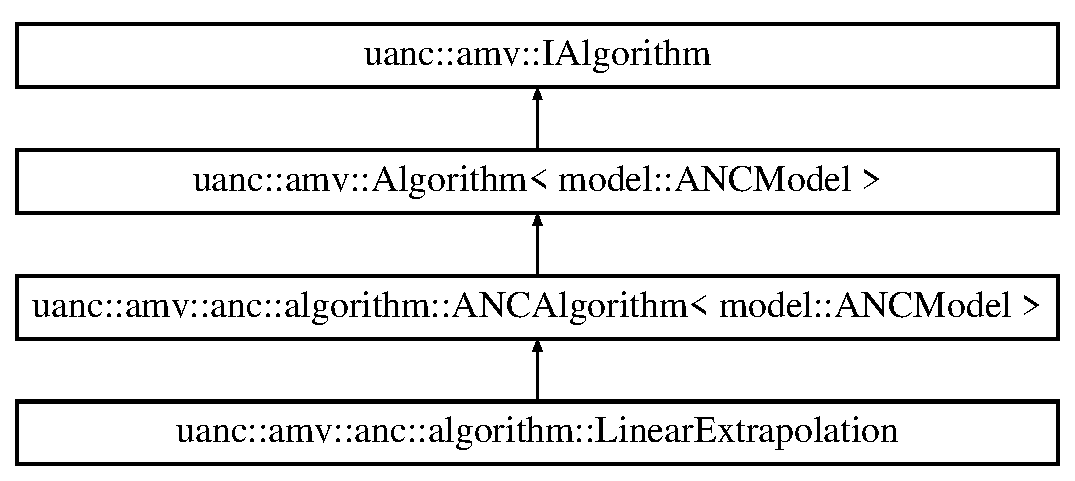
\includegraphics[height=4.000000cm]{classuanc_1_1amv_1_1anc_1_1algorithm_1_1_linear_extrapolation}
\end{center}
\end{figure}
\subsection*{Public Member Functions}
\begin{DoxyCompactItemize}
\item 
std\+::string \hyperlink{classuanc_1_1amv_1_1anc_1_1algorithm_1_1_linear_extrapolation_afc4328260d3f9c7d8a9be50df5a30e50}{get\+Name} () final
\begin{DoxyCompactList}\small\item\em Returns the name of the algorithm. \end{DoxyCompactList}\item 
void \hyperlink{classuanc_1_1amv_1_1anc_1_1algorithm_1_1_linear_extrapolation_aafb6717c9cb632241b10875630970388}{invert} (std\+::shared\+\_\+ptr$<$ \hyperlink{classuanc_1_1amv_1_1_inverted_model}{Inverted\+Model} $>$ in) final
\begin{DoxyCompactList}\small\item\em Inverts the input signal. \end{DoxyCompactList}\item 
\hyperlink{classuanc_1_1amv_1_1_algorithm}{Algorithm} $\ast$ \hyperlink{classuanc_1_1amv_1_1anc_1_1algorithm_1_1_linear_extrapolation_adbd3916228ea66603c4c5362f3392548}{clone} () final
\begin{DoxyCompactList}\small\item\em Clones the current instance. \end{DoxyCompactList}\end{DoxyCompactItemize}
\subsection*{Protected Member Functions}
\begin{DoxyCompactItemize}
\item 
\hyperlink{classuanc_1_1amv_1_1_algorithm_view}{Algorithm\+View}$<$ \hyperlink{classuanc_1_1amv_1_1anc_1_1model_1_1_a_n_c_model}{model\+::\+A\+N\+C\+Model} $>$ $\ast$ \hyperlink{classuanc_1_1amv_1_1anc_1_1algorithm_1_1_linear_extrapolation_a5cd4a27f8c92ab3f95f59cc8be260161}{construct\+View} () final
\begin{DoxyCompactList}\small\item\em Constructs a view, which can handle an A\+N\+C\+Model. \end{DoxyCompactList}\end{DoxyCompactItemize}


\subsection{Member Function Documentation}
\index{uanc\+::amv\+::anc\+::algorithm\+::\+Linear\+Extrapolation@{uanc\+::amv\+::anc\+::algorithm\+::\+Linear\+Extrapolation}!clone@{clone}}
\index{clone@{clone}!uanc\+::amv\+::anc\+::algorithm\+::\+Linear\+Extrapolation@{uanc\+::amv\+::anc\+::algorithm\+::\+Linear\+Extrapolation}}
\subsubsection[{\texorpdfstring{clone() final}{clone() final}}]{\setlength{\rightskip}{0pt plus 5cm}{\bf Algorithm}$\ast$ uanc\+::amv\+::anc\+::algorithm\+::\+Linear\+Extrapolation\+::clone (
\begin{DoxyParamCaption}
{}
\end{DoxyParamCaption}
)\hspace{0.3cm}{\ttfamily [inline]}, {\ttfamily [final]}, {\ttfamily [virtual]}}\hypertarget{classuanc_1_1amv_1_1anc_1_1algorithm_1_1_linear_extrapolation_adbd3916228ea66603c4c5362f3392548}{}\label{classuanc_1_1amv_1_1anc_1_1algorithm_1_1_linear_extrapolation_adbd3916228ea66603c4c5362f3392548}


Clones the current instance. 

This is basically the prototype pattern. It gets used to create an copy of the current \hyperlink{classuanc_1_1amv_1_1anc_1_1algorithm_1_1_inverse_direct_algorithm}{Inverse\+Direct\+Algorithm}. To do so it simply creates a new instance.

\begin{DoxyReturn}{Returns}
The cloned algorithm. 
\end{DoxyReturn}


Implements \hyperlink{classuanc_1_1amv_1_1_i_algorithm_af6fcbfa35f460363c2cc7e6134af8dc7}{uanc\+::amv\+::\+I\+Algorithm}.

\index{uanc\+::amv\+::anc\+::algorithm\+::\+Linear\+Extrapolation@{uanc\+::amv\+::anc\+::algorithm\+::\+Linear\+Extrapolation}!construct\+View@{construct\+View}}
\index{construct\+View@{construct\+View}!uanc\+::amv\+::anc\+::algorithm\+::\+Linear\+Extrapolation@{uanc\+::amv\+::anc\+::algorithm\+::\+Linear\+Extrapolation}}
\subsubsection[{\texorpdfstring{construct\+View() final}{constructView() final}}]{\setlength{\rightskip}{0pt plus 5cm}{\bf Algorithm\+View}$<${\bf model\+::\+A\+N\+C\+Model}$>$$\ast$ uanc\+::amv\+::anc\+::algorithm\+::\+Linear\+Extrapolation\+::construct\+View (
\begin{DoxyParamCaption}
{}
\end{DoxyParamCaption}
)\hspace{0.3cm}{\ttfamily [inline]}, {\ttfamily [final]}, {\ttfamily [protected]}, {\ttfamily [virtual]}}\hypertarget{classuanc_1_1amv_1_1anc_1_1algorithm_1_1_linear_extrapolation_a5cd4a27f8c92ab3f95f59cc8be260161}{}\label{classuanc_1_1amv_1_1anc_1_1algorithm_1_1_linear_extrapolation_a5cd4a27f8c92ab3f95f59cc8be260161}


Constructs a view, which can handle an A\+N\+C\+Model. 

This view basically display the standard information of the algorithm.

\begin{DoxyReturn}{Returns}
The created A\+N\+C\+View. 
\end{DoxyReturn}


Implements \hyperlink{classuanc_1_1amv_1_1_algorithm_af5561072283ed19634893263c95a4b6e}{uanc\+::amv\+::\+Algorithm$<$ model\+::\+A\+N\+C\+Model $>$}.

\index{uanc\+::amv\+::anc\+::algorithm\+::\+Linear\+Extrapolation@{uanc\+::amv\+::anc\+::algorithm\+::\+Linear\+Extrapolation}!get\+Name@{get\+Name}}
\index{get\+Name@{get\+Name}!uanc\+::amv\+::anc\+::algorithm\+::\+Linear\+Extrapolation@{uanc\+::amv\+::anc\+::algorithm\+::\+Linear\+Extrapolation}}
\subsubsection[{\texorpdfstring{get\+Name() final}{getName() final}}]{\setlength{\rightskip}{0pt plus 5cm}std\+::string uanc\+::amv\+::anc\+::algorithm\+::\+Linear\+Extrapolation\+::get\+Name (
\begin{DoxyParamCaption}
{}
\end{DoxyParamCaption}
)\hspace{0.3cm}{\ttfamily [inline]}, {\ttfamily [final]}, {\ttfamily [virtual]}}\hypertarget{classuanc_1_1amv_1_1anc_1_1algorithm_1_1_linear_extrapolation_afc4328260d3f9c7d8a9be50df5a30e50}{}\label{classuanc_1_1amv_1_1anc_1_1algorithm_1_1_linear_extrapolation_afc4328260d3f9c7d8a9be50df5a30e50}


Returns the name of the algorithm. 

Simply passes back the name of the algorithm.

\begin{DoxyReturn}{Returns}
Name of the algorithm 
\end{DoxyReturn}


Implements \hyperlink{classuanc_1_1amv_1_1_i_algorithm_a4935ab2fdacccf7df35d6fb596075edb}{uanc\+::amv\+::\+I\+Algorithm}.

\index{uanc\+::amv\+::anc\+::algorithm\+::\+Linear\+Extrapolation@{uanc\+::amv\+::anc\+::algorithm\+::\+Linear\+Extrapolation}!invert@{invert}}
\index{invert@{invert}!uanc\+::amv\+::anc\+::algorithm\+::\+Linear\+Extrapolation@{uanc\+::amv\+::anc\+::algorithm\+::\+Linear\+Extrapolation}}
\subsubsection[{\texorpdfstring{invert(std\+::shared\+\_\+ptr$<$ Inverted\+Model $>$ in) final}{invert(std::shared_ptr< InvertedModel > in) final}}]{\setlength{\rightskip}{0pt plus 5cm}void uanc\+::amv\+::anc\+::algorithm\+::\+Linear\+Extrapolation\+::invert (
\begin{DoxyParamCaption}
\item[{std\+::shared\+\_\+ptr$<$ {\bf Inverted\+Model} $>$}]{in}
\end{DoxyParamCaption}
)\hspace{0.3cm}{\ttfamily [inline]}, {\ttfamily [final]}, {\ttfamily [virtual]}}\hypertarget{classuanc_1_1amv_1_1anc_1_1algorithm_1_1_linear_extrapolation_aafb6717c9cb632241b10875630970388}{}\label{classuanc_1_1amv_1_1anc_1_1algorithm_1_1_linear_extrapolation_aafb6717c9cb632241b10875630970388}


Inverts the input signal. 

This is actually the heart of an A\+NC algorithm inside of this application. It takes an input model and processes it. Besides it should save its data inside the model using \hyperlink{classuanc_1_1amv_1_1anc_1_1algorithm_1_1_a_n_c_algorithm_a12ce80f6746cbb440cf771fc6878f7cf}{get\+Model()}.


\begin{DoxyParams}{Parameters}
{\em input} & The input model containing the original signal. \\
\hline
\end{DoxyParams}


Implements \hyperlink{classuanc_1_1amv_1_1anc_1_1algorithm_1_1_a_n_c_algorithm_abfdc7f14f7e41e408ee08037a839760d}{uanc\+::amv\+::anc\+::algorithm\+::\+A\+N\+C\+Algorithm$<$ model\+::\+A\+N\+C\+Model $>$}.



The documentation for this class was generated from the following file\+:\begin{DoxyCompactItemize}
\item 
/ext/local/\+University/\+B\+P/\+Git/\+U\+A\+N\+C/\+Code/\+U\+A\+N\+C/amv/anc/algorithm/\hyperlink{_linear_extrapolation_8h}{Linear\+Extrapolation.\+h}\end{DoxyCompactItemize}

\hypertarget{classuanc_1_1gui_1_1_main_widget}{}\section{uanc\+:\+:gui\+:\+:Main\+Widget Class Reference}
\label{classuanc_1_1gui_1_1_main_widget}\index{uanc\+::gui\+::\+Main\+Widget@{uanc\+::gui\+::\+Main\+Widget}}


{\ttfamily \#include $<$Main\+Widget.\+h$>$}

Inheritance diagram for uanc\+:\+:gui\+:\+:Main\+Widget\+:\begin{figure}[H]
\begin{center}
\leavevmode
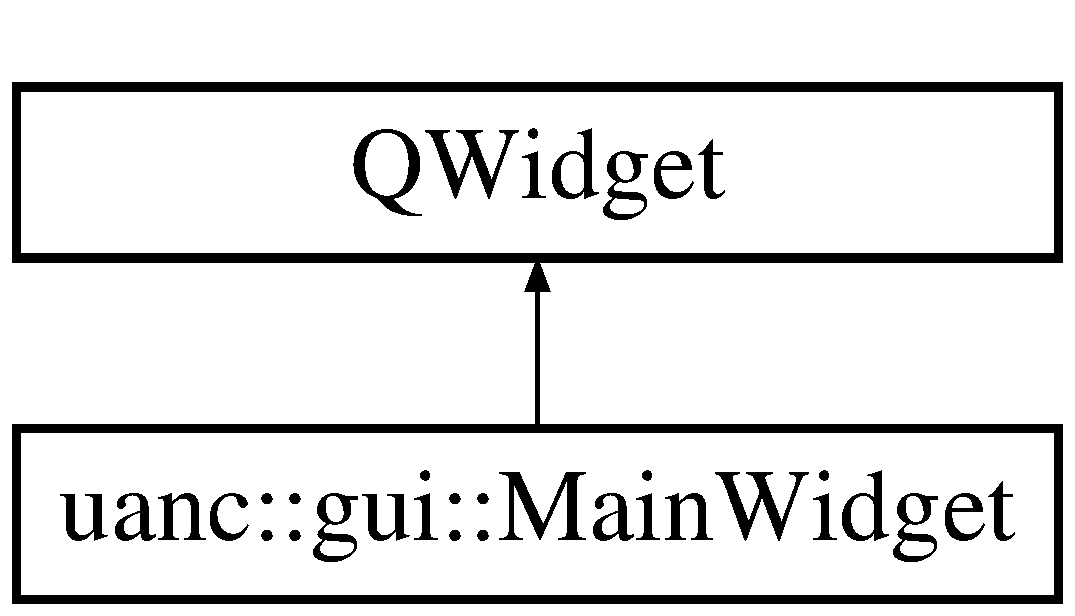
\includegraphics[height=2.000000cm]{classuanc_1_1gui_1_1_main_widget}
\end{center}
\end{figure}
\subsection*{Public Slots}
\begin{DoxyCompactItemize}
\item 
void \hyperlink{classuanc_1_1gui_1_1_main_widget_ac2e8a417bf4e8b90b707168a9dc65642}{algorithm\+Finished} ()
\item 
void \hyperlink{classuanc_1_1gui_1_1_main_widget_a2c4e4db69935d33facd4280e7dd66b05}{apply\+Clicked} ()
\begin{DoxyCompactList}\small\item\em This gets fired, when the apply button is clicked. \end{DoxyCompactList}\item 
void \hyperlink{classuanc_1_1gui_1_1_main_widget_a3e724b26e32f136b0e8f443075ec05e1}{tab\+Selected} ()
\begin{DoxyCompactList}\small\item\em Simple signal for a differenct selected tab. \end{DoxyCompactList}\item 
void \hyperlink{classuanc_1_1gui_1_1_main_widget_a210dbd2254febbd5e356e0b0a955f052}{wave\+Closed} (const int \&index)
\begin{DoxyCompactList}\small\item\em This gets fired, when a wave tab is closed. \end{DoxyCompactList}\item 
void \hyperlink{classuanc_1_1gui_1_1_main_widget_a01f7a68c0a5fb934183710176625cac4}{algorithm\+Closed} (const int \&index)
\begin{DoxyCompactList}\small\item\em This gets fired, when a algorithm tab is closed. \end{DoxyCompactList}\end{DoxyCompactItemize}
\subsection*{Public Member Functions}
\begin{DoxyCompactItemize}
\item 
\hyperlink{classuanc_1_1gui_1_1_main_widget_ac008ef19dc126b99cb36957d4f8725e9}{Main\+Widget} ()
\begin{DoxyCompactList}\small\item\em This is the main widget constructor. \end{DoxyCompactList}\item 
void \hyperlink{classuanc_1_1gui_1_1_main_widget_a5de87dc6cfeb353120647948893431a9}{load\+Signal\+Source} (std\+::shared\+\_\+ptr$<$ \hyperlink{classuanc_1_1amv_1_1_inverted_model}{Inverted\+Model} $>$ signal\+Source)
\begin{DoxyCompactList}\small\item\em loads the signal source. \end{DoxyCompactList}\end{DoxyCompactItemize}


\subsection{Constructor \& Destructor Documentation}
\index{uanc\+::gui\+::\+Main\+Widget@{uanc\+::gui\+::\+Main\+Widget}!Main\+Widget@{Main\+Widget}}
\index{Main\+Widget@{Main\+Widget}!uanc\+::gui\+::\+Main\+Widget@{uanc\+::gui\+::\+Main\+Widget}}
\subsubsection[{\texorpdfstring{Main\+Widget()}{MainWidget()}}]{\setlength{\rightskip}{0pt plus 5cm}uanc\+::gui\+::\+Main\+Widget\+::\+Main\+Widget (
\begin{DoxyParamCaption}
{}
\end{DoxyParamCaption}
)}\hypertarget{classuanc_1_1gui_1_1_main_widget_ac008ef19dc126b99cb36957d4f8725e9}{}\label{classuanc_1_1gui_1_1_main_widget_ac008ef19dc126b99cb36957d4f8725e9}


This is the main widget constructor. 

This basically initializes the gui and does some other initialization stuff. 

\subsection{Member Function Documentation}
\index{uanc\+::gui\+::\+Main\+Widget@{uanc\+::gui\+::\+Main\+Widget}!algorithm\+Closed@{algorithm\+Closed}}
\index{algorithm\+Closed@{algorithm\+Closed}!uanc\+::gui\+::\+Main\+Widget@{uanc\+::gui\+::\+Main\+Widget}}
\subsubsection[{\texorpdfstring{algorithm\+Closed}{algorithmClosed}}]{\setlength{\rightskip}{0pt plus 5cm}void uanc\+::gui\+::\+Main\+Widget\+::algorithm\+Closed (
\begin{DoxyParamCaption}
\item[{const int \&}]{index}
\end{DoxyParamCaption}
)\hspace{0.3cm}{\ttfamily [slot]}}\hypertarget{classuanc_1_1gui_1_1_main_widget_a01f7a68c0a5fb934183710176625cac4}{}\label{classuanc_1_1gui_1_1_main_widget_a01f7a68c0a5fb934183710176625cac4}


This gets fired, when a algorithm tab is closed. 

This gets fired, when a algorithm tab is closed. \index{uanc\+::gui\+::\+Main\+Widget@{uanc\+::gui\+::\+Main\+Widget}!algorithm\+Finished@{algorithm\+Finished}}
\index{algorithm\+Finished@{algorithm\+Finished}!uanc\+::gui\+::\+Main\+Widget@{uanc\+::gui\+::\+Main\+Widget}}
\subsubsection[{\texorpdfstring{algorithm\+Finished}{algorithmFinished}}]{\setlength{\rightskip}{0pt plus 5cm}void uanc\+::gui\+::\+Main\+Widget\+::algorithm\+Finished (
\begin{DoxyParamCaption}
{}
\end{DoxyParamCaption}
)\hspace{0.3cm}{\ttfamily [slot]}}\hypertarget{classuanc_1_1gui_1_1_main_widget_ac2e8a417bf4e8b90b707168a9dc65642}{}\label{classuanc_1_1gui_1_1_main_widget_ac2e8a417bf4e8b90b707168a9dc65642}
Gets called when the algorithm is finished. \index{uanc\+::gui\+::\+Main\+Widget@{uanc\+::gui\+::\+Main\+Widget}!apply\+Clicked@{apply\+Clicked}}
\index{apply\+Clicked@{apply\+Clicked}!uanc\+::gui\+::\+Main\+Widget@{uanc\+::gui\+::\+Main\+Widget}}
\subsubsection[{\texorpdfstring{apply\+Clicked}{applyClicked}}]{\setlength{\rightskip}{0pt plus 5cm}void uanc\+::gui\+::\+Main\+Widget\+::apply\+Clicked (
\begin{DoxyParamCaption}
{}
\end{DoxyParamCaption}
)\hspace{0.3cm}{\ttfamily [slot]}}\hypertarget{classuanc_1_1gui_1_1_main_widget_a2c4e4db69935d33facd4280e7dd66b05}{}\label{classuanc_1_1gui_1_1_main_widget_a2c4e4db69935d33facd4280e7dd66b05}


This gets fired, when the apply button is clicked. 

This gets fired, when the direct inverse button is clicked.

Gets fired, whenever a user clicks on the apply button.

Gets fired, whenever a user clicks on the direct inverse button. \index{uanc\+::gui\+::\+Main\+Widget@{uanc\+::gui\+::\+Main\+Widget}!load\+Signal\+Source@{load\+Signal\+Source}}
\index{load\+Signal\+Source@{load\+Signal\+Source}!uanc\+::gui\+::\+Main\+Widget@{uanc\+::gui\+::\+Main\+Widget}}
\subsubsection[{\texorpdfstring{load\+Signal\+Source(std\+::shared\+\_\+ptr$<$ Inverted\+Model $>$ signal\+Source)}{loadSignalSource(std::shared_ptr< InvertedModel > signalSource)}}]{\setlength{\rightskip}{0pt plus 5cm}void uanc\+::gui\+::\+Main\+Widget\+::load\+Signal\+Source (
\begin{DoxyParamCaption}
\item[{std\+::shared\+\_\+ptr$<$ {\bf Inverted\+Model} $>$}]{signal\+Source}
\end{DoxyParamCaption}
)}\hypertarget{classuanc_1_1gui_1_1_main_widget_a5de87dc6cfeb353120647948893431a9}{}\label{classuanc_1_1gui_1_1_main_widget_a5de87dc6cfeb353120647948893431a9}


loads the signal source. 

This method loads a signal source in the top tab view. 
\begin{DoxyParams}{Parameters}
{\em signal\+Source} & the signal source to load. \\
\hline
\end{DoxyParams}
\index{uanc\+::gui\+::\+Main\+Widget@{uanc\+::gui\+::\+Main\+Widget}!tab\+Selected@{tab\+Selected}}
\index{tab\+Selected@{tab\+Selected}!uanc\+::gui\+::\+Main\+Widget@{uanc\+::gui\+::\+Main\+Widget}}
\subsubsection[{\texorpdfstring{tab\+Selected}{tabSelected}}]{\setlength{\rightskip}{0pt plus 5cm}void uanc\+::gui\+::\+Main\+Widget\+::tab\+Selected (
\begin{DoxyParamCaption}
{}
\end{DoxyParamCaption}
)\hspace{0.3cm}{\ttfamily [slot]}}\hypertarget{classuanc_1_1gui_1_1_main_widget_a3e724b26e32f136b0e8f443075ec05e1}{}\label{classuanc_1_1gui_1_1_main_widget_a3e724b26e32f136b0e8f443075ec05e1}


Simple signal for a differenct selected tab. 

\index{uanc\+::gui\+::\+Main\+Widget@{uanc\+::gui\+::\+Main\+Widget}!wave\+Closed@{wave\+Closed}}
\index{wave\+Closed@{wave\+Closed}!uanc\+::gui\+::\+Main\+Widget@{uanc\+::gui\+::\+Main\+Widget}}
\subsubsection[{\texorpdfstring{wave\+Closed}{waveClosed}}]{\setlength{\rightskip}{0pt plus 5cm}void uanc\+::gui\+::\+Main\+Widget\+::wave\+Closed (
\begin{DoxyParamCaption}
\item[{const int \&}]{index}
\end{DoxyParamCaption}
)\hspace{0.3cm}{\ttfamily [slot]}}\hypertarget{classuanc_1_1gui_1_1_main_widget_a210dbd2254febbd5e356e0b0a955f052}{}\label{classuanc_1_1gui_1_1_main_widget_a210dbd2254febbd5e356e0b0a955f052}


This gets fired, when a wave tab is closed. 

This gets fired, when a wave tab is closed. 

The documentation for this class was generated from the following files\+:\begin{DoxyCompactItemize}
\item 
/home/kurt/\+Documents/\+Studium/\+Bachelor\+\_\+\+Praktikum/\+U\+A\+N\+C/\+Code/\+U\+A\+N\+C/gui/\hyperlink{_main_widget_8h}{Main\+Widget.\+h}\item 
/home/kurt/\+Documents/\+Studium/\+Bachelor\+\_\+\+Praktikum/\+U\+A\+N\+C/\+Code/\+U\+A\+N\+C/gui/\hyperlink{_main_widget_8cpp}{Main\+Widget.\+cpp}\end{DoxyCompactItemize}

\hypertarget{classuanc_1_1gui_1_1_main_window}{}\section{uanc\+:\+:gui\+:\+:Main\+Window Class Reference}
\label{classuanc_1_1gui_1_1_main_window}\index{uanc\+::gui\+::\+Main\+Window@{uanc\+::gui\+::\+Main\+Window}}


This class represents the main window.  




{\ttfamily \#include $<$Main\+Window.\+h$>$}

Inheritance diagram for uanc\+:\+:gui\+:\+:Main\+Window\+:\begin{figure}[H]
\begin{center}
\leavevmode
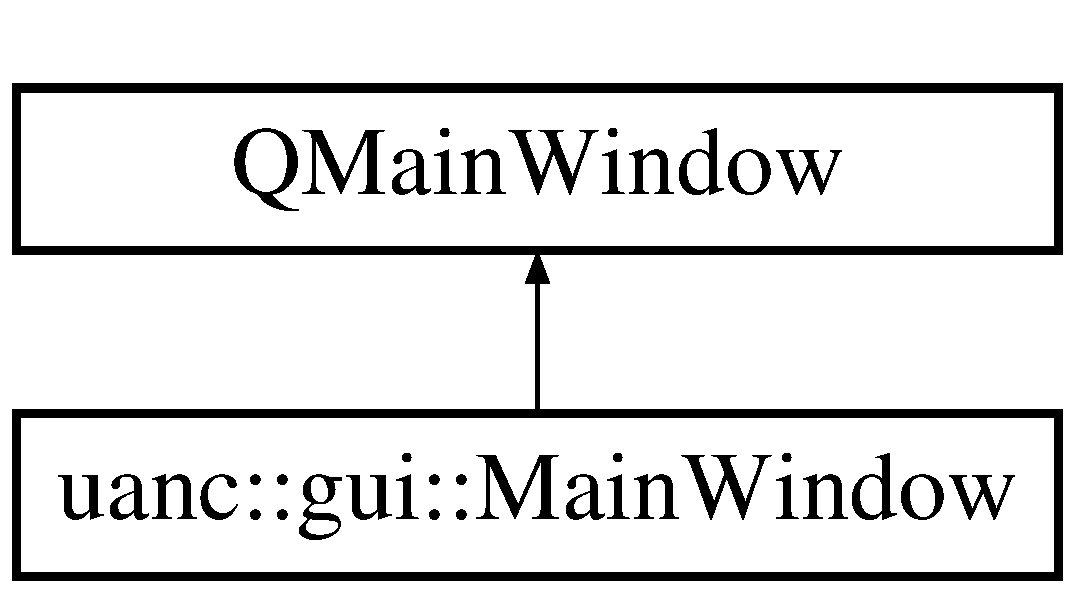
\includegraphics[height=2.000000cm]{classuanc_1_1gui_1_1_main_window}
\end{center}
\end{figure}
\subsection*{Static Public Member Functions}
\begin{DoxyCompactItemize}
\item 
static \hyperlink{classuanc_1_1gui_1_1_main_window}{Main\+Window} $\ast$ \hyperlink{classuanc_1_1gui_1_1_main_window_ae3833ff9b8d0e1feb996ce009887f239}{get} ()
\begin{DoxyCompactList}\small\item\em Hol a reference to the main window. \end{DoxyCompactList}\end{DoxyCompactItemize}
\subsection*{Protected Member Functions}
\begin{DoxyCompactItemize}
\item 
void \hyperlink{classuanc_1_1gui_1_1_main_window_a523b741dd8f49b3dfaf8a66bd76a254b}{close\+Event} (Q\+Close\+Event $\ast$)
\begin{DoxyCompactList}\small\item\em This method executes all necessary actions when the main application is closed. \end{DoxyCompactList}\end{DoxyCompactItemize}


\subsection{Detailed Description}
This class represents the main window. 

It is a Q\+Main\+Window. So you can think of it as a wrapper to extend the functionality of a basic Q\+Main\+Window 

\subsection{Member Function Documentation}
\index{uanc\+::gui\+::\+Main\+Window@{uanc\+::gui\+::\+Main\+Window}!close\+Event@{close\+Event}}
\index{close\+Event@{close\+Event}!uanc\+::gui\+::\+Main\+Window@{uanc\+::gui\+::\+Main\+Window}}
\subsubsection[{\texorpdfstring{close\+Event(\+Q\+Close\+Event $\ast$)}{closeEvent(QCloseEvent *)}}]{\setlength{\rightskip}{0pt plus 5cm}void uanc\+::gui\+::\+Main\+Window\+::close\+Event (
\begin{DoxyParamCaption}
\item[{Q\+Close\+Event $\ast$}]{}
\end{DoxyParamCaption}
)\hspace{0.3cm}{\ttfamily [protected]}}\hypertarget{classuanc_1_1gui_1_1_main_window_a523b741dd8f49b3dfaf8a66bd76a254b}{}\label{classuanc_1_1gui_1_1_main_window_a523b741dd8f49b3dfaf8a66bd76a254b}


This method executes all necessary actions when the main application is closed. 

It executes all necessary actions when the main application is closed \index{uanc\+::gui\+::\+Main\+Window@{uanc\+::gui\+::\+Main\+Window}!get@{get}}
\index{get@{get}!uanc\+::gui\+::\+Main\+Window@{uanc\+::gui\+::\+Main\+Window}}
\subsubsection[{\texorpdfstring{get()}{get()}}]{\setlength{\rightskip}{0pt plus 5cm}{\bf Main\+Window} $\ast$ uanc\+::gui\+::\+Main\+Window\+::get (
\begin{DoxyParamCaption}
{}
\end{DoxyParamCaption}
)\hspace{0.3cm}{\ttfamily [static]}}\hypertarget{classuanc_1_1gui_1_1_main_window_ae3833ff9b8d0e1feb996ce009887f239}{}\label{classuanc_1_1gui_1_1_main_window_ae3833ff9b8d0e1feb996ce009887f239}


Hol a reference to the main window. 

Obtain a reference to the main window.

Uses a classical singleton pattern to give back exactly the same copy of the main window. In addition it uses a shared pointer.

\begin{DoxyReturn}{Returns}
The shared pointer containing the \hyperlink{classuanc_1_1gui_1_1_main_window}{Main\+Window} 
\end{DoxyReturn}


The documentation for this class was generated from the following files\+:\begin{DoxyCompactItemize}
\item 
/ext/local/\+University/\+B\+P/\+Git/\+U\+A\+N\+C/\+Code/\+U\+A\+N\+C/gui/\hyperlink{_main_window_8h}{Main\+Window.\+h}\item 
/ext/local/\+University/\+B\+P/\+Git/\+U\+A\+N\+C/\+Code/\+U\+A\+N\+C/gui/\hyperlink{_main_window_8cpp}{Main\+Window.\+cpp}\end{DoxyCompactItemize}

\hypertarget{classuanc_1_1util_1_1_path}{}\section{uanc\+:\+:util\+:\+:Path Class Reference}
\label{classuanc_1_1util_1_1_path}\index{uanc\+::util\+::\+Path@{uanc\+::util\+::\+Path}}


{\ttfamily \#include $<$Path.\+h$>$}

\subsection*{Static Public Member Functions}
\begin{DoxyCompactItemize}
\item 
static std\+::string \hyperlink{classuanc_1_1util_1_1_path_a1b4b6ea0a432ae929367981260e79588}{get\+File\+Name} (std\+::string path)
\begin{DoxyCompactList}\small\item\em Passes back the filename of the given path. \end{DoxyCompactList}\end{DoxyCompactItemize}


\subsection{Member Function Documentation}
\index{uanc\+::util\+::\+Path@{uanc\+::util\+::\+Path}!get\+File\+Name@{get\+File\+Name}}
\index{get\+File\+Name@{get\+File\+Name}!uanc\+::util\+::\+Path@{uanc\+::util\+::\+Path}}
\subsubsection[{\texorpdfstring{get\+File\+Name(std\+::string path)}{getFileName(std::string path)}}]{\setlength{\rightskip}{0pt plus 5cm}std\+::string uanc\+::util\+::\+Path\+::get\+File\+Name (
\begin{DoxyParamCaption}
\item[{std\+::string}]{path}
\end{DoxyParamCaption}
)\hspace{0.3cm}{\ttfamily [static]}}\hypertarget{classuanc_1_1util_1_1_path_a1b4b6ea0a432ae929367981260e79588}{}\label{classuanc_1_1util_1_1_path_a1b4b6ea0a432ae929367981260e79588}


Passes back the filename of the given path. 



The documentation for this class was generated from the following files\+:\begin{DoxyCompactItemize}
\item 
/home/kurt/\+Documents/\+Studium/\+Bachelor\+\_\+\+Praktikum/\+U\+A\+N\+C/\+Code/\+U\+A\+N\+C/util/tools/\hyperlink{_path_8h}{Path.\+h}\item 
/home/kurt/\+Documents/\+Studium/\+Bachelor\+\_\+\+Praktikum/\+U\+A\+N\+C/\+Code/\+U\+A\+N\+C/util/tools/\hyperlink{_path_8cpp}{Path.\+cpp}\end{DoxyCompactItemize}

\hypertarget{classuanc_1_1util_1_1_performance_measure}{}\section{uanc\+:\+:util\+:\+:Performance\+Measure$<$ duration\+Type $>$ Class Template Reference}
\label{classuanc_1_1util_1_1_performance_measure}\index{uanc\+::util\+::\+Performance\+Measure$<$ duration\+Type $>$@{uanc\+::util\+::\+Performance\+Measure$<$ duration\+Type $>$}}


{\ttfamily \#include $<$Performance\+Measure.\+h$>$}

\subsection*{Public Member Functions}
\begin{DoxyCompactItemize}
\item 
const std\+::shared\+\_\+ptr$<$ \hyperlink{classuanc_1_1util_1_1_performance_measure_node}{Performance\+Measure\+Node}$<$ duration\+Type $>$ $>$ \hyperlink{classuanc_1_1util_1_1_performance_measure_a851457bc741e9f21c1e8f949fc17c2bf}{get\+Root\+Measure} () const 
\item 
void \hyperlink{classuanc_1_1util_1_1_performance_measure_a63d1c53616c602fa930f2b17b50d7604}{start} (std\+::string title)
\item 
void \hyperlink{classuanc_1_1util_1_1_performance_measure_a5ce9bf037e972cb7adad94e0312e7504}{restart} ()
\item 
void \hyperlink{classuanc_1_1util_1_1_performance_measure_a6931b89f739c6f334b59e85a2b3ce5b8}{stop} ()
\item 
void \hyperlink{classuanc_1_1util_1_1_performance_measure_a7284b6620e998084b6cd548cb0b5c6c3}{start\+Sub\+Measure} (std\+::string sub\+Measure\+Title=\char`\"{}\char`\"{})
\item 
void \hyperlink{classuanc_1_1util_1_1_performance_measure_a82db8e78171d1dfbe4af7fda3fe67a54}{stop\+Sub\+Measure} ()
\item 
void \hyperlink{classuanc_1_1util_1_1_performance_measure_a0d5a7a487a2db18a748d17867e58b053}{stop\+All\+Measurements} ()
\end{DoxyCompactItemize}


\subsection{Detailed Description}
\subsubsection*{template$<$typename duration\+Type = std\+::chrono\+::microseconds$>$\\*
class uanc\+::util\+::\+Performance\+Measure$<$ duration\+Type $>$}

Class for the performance measure of algorithms.

It creates a 2 -\/ dimensional tree, where subsequent measurements are stored in the horizontal and sub-\/measures are stored in the vertical dimension. A measure main contain multiple sub-\/measure layers.


\begin{DoxyPre}
 \hyperlink{classuanc_1_1util_1_1_performance_measure_a7284b6620e998084b6cd548cb0b5c6c3}{startSubMeasure()}.----.    \hyperlink{classuanc_1_1util_1_1_performance_measure_a63d1c53616c602fa930f2b17b50d7604}{start()}         .----.
    .-------------| M1 |------------------->| M2 |
    |             '----'                    '----'
    |               ^                       |   ^
    |               |                       |   |
    |               | \hyperlink{classuanc_1_1util_1_1_performance_measure_a82db8e78171d1dfbe4af7fda3fe67a54}{stopSubMeasure()}      |   |
    |               '------------------.    '---'
    v                                  |    \hyperlink{classuanc_1_1util_1_1_performance_measure_a6931b89f739c6f334b59e85a2b3ce5b8}{stop()}
 .----.       .----.                .----.
 | S1 |------>| S2 |--------------->| S3 |
 '----'       '----'                '----'
       \hyperlink{classuanc_1_1util_1_1_performance_measure_a63d1c53616c602fa930f2b17b50d7604}{start()}          \hyperlink{classuanc_1_1util_1_1_performance_measure_a63d1c53616c602fa930f2b17b50d7604}{start()}
\end{DoxyPre}
 

\subsection{Member Function Documentation}
\index{uanc\+::util\+::\+Performance\+Measure@{uanc\+::util\+::\+Performance\+Measure}!get\+Root\+Measure@{get\+Root\+Measure}}
\index{get\+Root\+Measure@{get\+Root\+Measure}!uanc\+::util\+::\+Performance\+Measure@{uanc\+::util\+::\+Performance\+Measure}}
\subsubsection[{\texorpdfstring{get\+Root\+Measure() const }{getRootMeasure() const }}]{\setlength{\rightskip}{0pt plus 5cm}template$<$typename duration\+Type  = std\+::chrono\+::microseconds$>$ const std\+::shared\+\_\+ptr$<${\bf Performance\+Measure\+Node}$<$duration\+Type$>$ $>$ {\bf uanc\+::util\+::\+Performance\+Measure}$<$ duration\+Type $>$\+::get\+Root\+Measure (
\begin{DoxyParamCaption}
{}
\end{DoxyParamCaption}
) const\hspace{0.3cm}{\ttfamily [inline]}}\hypertarget{classuanc_1_1util_1_1_performance_measure_a851457bc741e9f21c1e8f949fc17c2bf}{}\label{classuanc_1_1util_1_1_performance_measure_a851457bc741e9f21c1e8f949fc17c2bf}
Returns a pointer to the root measurement node. \begin{DoxyReturn}{Returns}
The pointer to the root measurement node 
\end{DoxyReturn}
\index{uanc\+::util\+::\+Performance\+Measure@{uanc\+::util\+::\+Performance\+Measure}!restart@{restart}}
\index{restart@{restart}!uanc\+::util\+::\+Performance\+Measure@{uanc\+::util\+::\+Performance\+Measure}}
\subsubsection[{\texorpdfstring{restart()}{restart()}}]{\setlength{\rightskip}{0pt plus 5cm}template$<$typename duration\+Type  = std\+::chrono\+::microseconds$>$ void {\bf uanc\+::util\+::\+Performance\+Measure}$<$ duration\+Type $>$\+::restart (
\begin{DoxyParamCaption}
{}
\end{DoxyParamCaption}
)\hspace{0.3cm}{\ttfamily [inline]}}\hypertarget{classuanc_1_1util_1_1_performance_measure_a5ce9bf037e972cb7adad94e0312e7504}{}\label{classuanc_1_1util_1_1_performance_measure_a5ce9bf037e972cb7adad94e0312e7504}
Restarts the current measurement without creating a new measurement node. \index{uanc\+::util\+::\+Performance\+Measure@{uanc\+::util\+::\+Performance\+Measure}!start@{start}}
\index{start@{start}!uanc\+::util\+::\+Performance\+Measure@{uanc\+::util\+::\+Performance\+Measure}}
\subsubsection[{\texorpdfstring{start(std\+::string title)}{start(std::string title)}}]{\setlength{\rightskip}{0pt plus 5cm}template$<$typename duration\+Type  = std\+::chrono\+::microseconds$>$ void {\bf uanc\+::util\+::\+Performance\+Measure}$<$ duration\+Type $>$\+::start (
\begin{DoxyParamCaption}
\item[{std\+::string}]{title}
\end{DoxyParamCaption}
)\hspace{0.3cm}{\ttfamily [inline]}}\hypertarget{classuanc_1_1util_1_1_performance_measure_a63d1c53616c602fa930f2b17b50d7604}{}\label{classuanc_1_1util_1_1_performance_measure_a63d1c53616c602fa930f2b17b50d7604}
Starts a new measurement or sub-\/measurement. A new node is created, w \index{uanc\+::util\+::\+Performance\+Measure@{uanc\+::util\+::\+Performance\+Measure}!start\+Sub\+Measure@{start\+Sub\+Measure}}
\index{start\+Sub\+Measure@{start\+Sub\+Measure}!uanc\+::util\+::\+Performance\+Measure@{uanc\+::util\+::\+Performance\+Measure}}
\subsubsection[{\texorpdfstring{start\+Sub\+Measure(std\+::string sub\+Measure\+Title="""")}{startSubMeasure(std::string subMeasureTitle="")}}]{\setlength{\rightskip}{0pt plus 5cm}template$<$typename duration\+Type  = std\+::chrono\+::microseconds$>$ void {\bf uanc\+::util\+::\+Performance\+Measure}$<$ duration\+Type $>$\+::start\+Sub\+Measure (
\begin{DoxyParamCaption}
\item[{std\+::string}]{sub\+Measure\+Title = {\ttfamily \char`\"{}\char`\"{}}}
\end{DoxyParamCaption}
)\hspace{0.3cm}{\ttfamily [inline]}}\hypertarget{classuanc_1_1util_1_1_performance_measure_a7284b6620e998084b6cd548cb0b5c6c3}{}\label{classuanc_1_1util_1_1_performance_measure_a7284b6620e998084b6cd548cb0b5c6c3}
Starts a new sub-\/measure layer with a measure with the given title. The sub-\/measure is started immediately. 
\begin{DoxyParams}{Parameters}
{\em sub\+Measure\+Title} & The title of the sub-\/measurement. \\
\hline
\end{DoxyParams}
\index{uanc\+::util\+::\+Performance\+Measure@{uanc\+::util\+::\+Performance\+Measure}!stop@{stop}}
\index{stop@{stop}!uanc\+::util\+::\+Performance\+Measure@{uanc\+::util\+::\+Performance\+Measure}}
\subsubsection[{\texorpdfstring{stop()}{stop()}}]{\setlength{\rightskip}{0pt plus 5cm}template$<$typename duration\+Type  = std\+::chrono\+::microseconds$>$ void {\bf uanc\+::util\+::\+Performance\+Measure}$<$ duration\+Type $>$\+::stop (
\begin{DoxyParamCaption}
{}
\end{DoxyParamCaption}
)\hspace{0.3cm}{\ttfamily [inline]}}\hypertarget{classuanc_1_1util_1_1_performance_measure_a6931b89f739c6f334b59e85a2b3ce5b8}{}\label{classuanc_1_1util_1_1_performance_measure_a6931b89f739c6f334b59e85a2b3ce5b8}
Stops the current measurement and saves its time \index{uanc\+::util\+::\+Performance\+Measure@{uanc\+::util\+::\+Performance\+Measure}!stop\+All\+Measurements@{stop\+All\+Measurements}}
\index{stop\+All\+Measurements@{stop\+All\+Measurements}!uanc\+::util\+::\+Performance\+Measure@{uanc\+::util\+::\+Performance\+Measure}}
\subsubsection[{\texorpdfstring{stop\+All\+Measurements()}{stopAllMeasurements()}}]{\setlength{\rightskip}{0pt plus 5cm}template$<$typename duration\+Type  = std\+::chrono\+::microseconds$>$ void {\bf uanc\+::util\+::\+Performance\+Measure}$<$ duration\+Type $>$\+::stop\+All\+Measurements (
\begin{DoxyParamCaption}
{}
\end{DoxyParamCaption}
)\hspace{0.3cm}{\ttfamily [inline]}}\hypertarget{classuanc_1_1util_1_1_performance_measure_a0d5a7a487a2db18a748d17867e58b053}{}\label{classuanc_1_1util_1_1_performance_measure_a0d5a7a487a2db18a748d17867e58b053}
Stops all running measurements and returns to the root measurement. \index{uanc\+::util\+::\+Performance\+Measure@{uanc\+::util\+::\+Performance\+Measure}!stop\+Sub\+Measure@{stop\+Sub\+Measure}}
\index{stop\+Sub\+Measure@{stop\+Sub\+Measure}!uanc\+::util\+::\+Performance\+Measure@{uanc\+::util\+::\+Performance\+Measure}}
\subsubsection[{\texorpdfstring{stop\+Sub\+Measure()}{stopSubMeasure()}}]{\setlength{\rightskip}{0pt plus 5cm}template$<$typename duration\+Type  = std\+::chrono\+::microseconds$>$ void {\bf uanc\+::util\+::\+Performance\+Measure}$<$ duration\+Type $>$\+::stop\+Sub\+Measure (
\begin{DoxyParamCaption}
{}
\end{DoxyParamCaption}
)\hspace{0.3cm}{\ttfamily [inline]}}\hypertarget{classuanc_1_1util_1_1_performance_measure_a82db8e78171d1dfbe4af7fda3fe67a54}{}\label{classuanc_1_1util_1_1_performance_measure_a82db8e78171d1dfbe4af7fda3fe67a54}
Stops the current measurement, if running, and returns to its parent. The parents state is not changed If no parent measurement exists, then nothing is done. 

The documentation for this class was generated from the following file\+:\begin{DoxyCompactItemize}
\item 
/home/kurt/\+Documents/\+Studium/\+Bachelor\+\_\+\+Praktikum/\+U\+A\+N\+C/\+Code/\+U\+A\+N\+C/util/\hyperlink{_performance_measure_8h}{Performance\+Measure.\+h}\end{DoxyCompactItemize}

\hypertarget{classuanc_1_1amv_1_1_p_m_register_1_1_performance_measurement_register}{}\section{uanc\+:\+:amv\+:\+:P\+M\+Register\+:\+:Performance\+Measurement\+Register Class Reference}
\label{classuanc_1_1amv_1_1_p_m_register_1_1_performance_measurement_register}\index{uanc\+::amv\+::\+P\+M\+Register\+::\+Performance\+Measurement\+Register@{uanc\+::amv\+::\+P\+M\+Register\+::\+Performance\+Measurement\+Register}}


This is an A\+N\+C\+Model.  




{\ttfamily \#include $<$Performance\+Measurement\+Register.\+h$>$}

\subsection*{Public Member Functions}
\begin{DoxyCompactItemize}
\item 
void \hyperlink{classuanc_1_1amv_1_1_p_m_register_1_1_performance_measurement_register_af790642629d149fc257d6541e674f2e8}{start\+Overall\+Execution\+Measurement} ()
\item 
void \hyperlink{classuanc_1_1amv_1_1_p_m_register_1_1_performance_measurement_register_a39c0be8c717c30eee29763a2e1e19848}{stop\+Overall\+Execution\+Measurement} ()
\item 
void \hyperlink{classuanc_1_1amv_1_1_p_m_register_1_1_performance_measurement_register_aa0950d36ffc0588844632034ebe5f473}{register\+Custom\+Measurement} (std\+::shared\+\_\+ptr$<$ \hyperlink{classuanc_1_1util_1_1_performance_measure}{util\+::\+Performance\+Measure}$<$$>$$>$ measurement)
\item 
const std\+::vector$<$ std\+::shared\+\_\+ptr$<$ \hyperlink{classuanc_1_1util_1_1_performance_measure}{util\+::\+Performance\+Measure}$<$$>$ $>$ $>$ \& \hyperlink{classuanc_1_1amv_1_1_p_m_register_1_1_performance_measurement_register_a461a8558d8b0358de9c6b3c6e9ba7f9e}{get\+Custom\+Measurements} () const 
\item 
const std\+::shared\+\_\+ptr$<$ \hyperlink{classuanc_1_1util_1_1_performance_measure}{util\+::\+Performance\+Measure}$<$$>$ $>$ \& \hyperlink{classuanc_1_1amv_1_1_p_m_register_1_1_performance_measurement_register_a764cef42743ad8c1655f9975f3782ec6}{get\+Overall\+Measurement} () const 
\end{DoxyCompactItemize}


\subsection{Detailed Description}
This is an A\+N\+C\+Model. 

This is the class for registering new Performance Measurements for an \hyperlink{classuanc_1_1amv_1_1_algorithm}{Algorithm}. It also contains the special default measurement which is executed for every class which inherits from A\+N\+C\+Algorithm. 

\subsection{Member Function Documentation}
\index{uanc\+::amv\+::\+P\+M\+Register\+::\+Performance\+Measurement\+Register@{uanc\+::amv\+::\+P\+M\+Register\+::\+Performance\+Measurement\+Register}!get\+Custom\+Measurements@{get\+Custom\+Measurements}}
\index{get\+Custom\+Measurements@{get\+Custom\+Measurements}!uanc\+::amv\+::\+P\+M\+Register\+::\+Performance\+Measurement\+Register@{uanc\+::amv\+::\+P\+M\+Register\+::\+Performance\+Measurement\+Register}}
\subsubsection[{\texorpdfstring{get\+Custom\+Measurements() const }{getCustomMeasurements() const }}]{\setlength{\rightskip}{0pt plus 5cm}const std\+::vector$<$std\+::shared\+\_\+ptr$<${\bf util\+::\+Performance\+Measure}$<$$>$ $>$ $>$\& uanc\+::amv\+::\+P\+M\+Register\+::\+Performance\+Measurement\+Register\+::get\+Custom\+Measurements (
\begin{DoxyParamCaption}
{}
\end{DoxyParamCaption}
) const\hspace{0.3cm}{\ttfamily [inline]}}\hypertarget{classuanc_1_1amv_1_1_p_m_register_1_1_performance_measurement_register_a461a8558d8b0358de9c6b3c6e9ba7f9e}{}\label{classuanc_1_1amv_1_1_p_m_register_1_1_performance_measurement_register_a461a8558d8b0358de9c6b3c6e9ba7f9e}
Give back the actual custom measurements \index{uanc\+::amv\+::\+P\+M\+Register\+::\+Performance\+Measurement\+Register@{uanc\+::amv\+::\+P\+M\+Register\+::\+Performance\+Measurement\+Register}!get\+Overall\+Measurement@{get\+Overall\+Measurement}}
\index{get\+Overall\+Measurement@{get\+Overall\+Measurement}!uanc\+::amv\+::\+P\+M\+Register\+::\+Performance\+Measurement\+Register@{uanc\+::amv\+::\+P\+M\+Register\+::\+Performance\+Measurement\+Register}}
\subsubsection[{\texorpdfstring{get\+Overall\+Measurement() const }{getOverallMeasurement() const }}]{\setlength{\rightskip}{0pt plus 5cm}const std\+::shared\+\_\+ptr$<${\bf util\+::\+Performance\+Measure}$<$$>$ $>$\& uanc\+::amv\+::\+P\+M\+Register\+::\+Performance\+Measurement\+Register\+::get\+Overall\+Measurement (
\begin{DoxyParamCaption}
{}
\end{DoxyParamCaption}
) const\hspace{0.3cm}{\ttfamily [inline]}}\hypertarget{classuanc_1_1amv_1_1_p_m_register_1_1_performance_measurement_register_a764cef42743ad8c1655f9975f3782ec6}{}\label{classuanc_1_1amv_1_1_p_m_register_1_1_performance_measurement_register_a764cef42743ad8c1655f9975f3782ec6}
Give back the overall measurment \index{uanc\+::amv\+::\+P\+M\+Register\+::\+Performance\+Measurement\+Register@{uanc\+::amv\+::\+P\+M\+Register\+::\+Performance\+Measurement\+Register}!register\+Custom\+Measurement@{register\+Custom\+Measurement}}
\index{register\+Custom\+Measurement@{register\+Custom\+Measurement}!uanc\+::amv\+::\+P\+M\+Register\+::\+Performance\+Measurement\+Register@{uanc\+::amv\+::\+P\+M\+Register\+::\+Performance\+Measurement\+Register}}
\subsubsection[{\texorpdfstring{register\+Custom\+Measurement(std\+::shared\+\_\+ptr$<$ util\+::\+Performance\+Measure$<$$>$$>$ measurement)}{registerCustomMeasurement(std::shared_ptr< util::PerformanceMeasure<>> measurement)}}]{\setlength{\rightskip}{0pt plus 5cm}void uanc\+::amv\+::\+P\+M\+Register\+::\+Performance\+Measurement\+Register\+::register\+Custom\+Measurement (
\begin{DoxyParamCaption}
\item[{std\+::shared\+\_\+ptr$<$ {\bf util\+::\+Performance\+Measure}$<$$>$$>$}]{measurement}
\end{DoxyParamCaption}
)}\hypertarget{classuanc_1_1amv_1_1_p_m_register_1_1_performance_measurement_register_aa0950d36ffc0588844632034ebe5f473}{}\label{classuanc_1_1amv_1_1_p_m_register_1_1_performance_measurement_register_aa0950d36ffc0588844632034ebe5f473}
Registers a custom measurement. 
\begin{DoxyParams}{Parameters}
{\em measurement} & The pointer to new measurement to register. \\
\hline
\end{DoxyParams}
\index{uanc\+::amv\+::\+P\+M\+Register\+::\+Performance\+Measurement\+Register@{uanc\+::amv\+::\+P\+M\+Register\+::\+Performance\+Measurement\+Register}!start\+Overall\+Execution\+Measurement@{start\+Overall\+Execution\+Measurement}}
\index{start\+Overall\+Execution\+Measurement@{start\+Overall\+Execution\+Measurement}!uanc\+::amv\+::\+P\+M\+Register\+::\+Performance\+Measurement\+Register@{uanc\+::amv\+::\+P\+M\+Register\+::\+Performance\+Measurement\+Register}}
\subsubsection[{\texorpdfstring{start\+Overall\+Execution\+Measurement()}{startOverallExecutionMeasurement()}}]{\setlength{\rightskip}{0pt plus 5cm}void uanc\+::amv\+::\+P\+M\+Register\+::\+Performance\+Measurement\+Register\+::start\+Overall\+Execution\+Measurement (
\begin{DoxyParamCaption}
{}
\end{DoxyParamCaption}
)}\hypertarget{classuanc_1_1amv_1_1_p_m_register_1_1_performance_measurement_register_af790642629d149fc257d6541e674f2e8}{}\label{classuanc_1_1amv_1_1_p_m_register_1_1_performance_measurement_register_af790642629d149fc257d6541e674f2e8}
This starts the execution of the overall Execution Measurement. This may be only executed once. \index{uanc\+::amv\+::\+P\+M\+Register\+::\+Performance\+Measurement\+Register@{uanc\+::amv\+::\+P\+M\+Register\+::\+Performance\+Measurement\+Register}!stop\+Overall\+Execution\+Measurement@{stop\+Overall\+Execution\+Measurement}}
\index{stop\+Overall\+Execution\+Measurement@{stop\+Overall\+Execution\+Measurement}!uanc\+::amv\+::\+P\+M\+Register\+::\+Performance\+Measurement\+Register@{uanc\+::amv\+::\+P\+M\+Register\+::\+Performance\+Measurement\+Register}}
\subsubsection[{\texorpdfstring{stop\+Overall\+Execution\+Measurement()}{stopOverallExecutionMeasurement()}}]{\setlength{\rightskip}{0pt plus 5cm}void uanc\+::amv\+::\+P\+M\+Register\+::\+Performance\+Measurement\+Register\+::stop\+Overall\+Execution\+Measurement (
\begin{DoxyParamCaption}
{}
\end{DoxyParamCaption}
)}\hypertarget{classuanc_1_1amv_1_1_p_m_register_1_1_performance_measurement_register_a39c0be8c717c30eee29763a2e1e19848}{}\label{classuanc_1_1amv_1_1_p_m_register_1_1_performance_measurement_register_a39c0be8c717c30eee29763a2e1e19848}
Stops the overall execution measurement, if it is running 

The documentation for this class was generated from the following files\+:\begin{DoxyCompactItemize}
\item 
/ext/local/\+University/\+B\+P/\+Git/\+U\+A\+N\+C/\+Code/\+U\+A\+N\+C/amv/\hyperlink{_performance_measurement_register_8h}{Performance\+Measurement\+Register.\+h}\item 
/ext/local/\+University/\+B\+P/\+Git/\+U\+A\+N\+C/\+Code/\+U\+A\+N\+C/amv/\hyperlink{_performance_measurement_register_8cpp}{Performance\+Measurement\+Register.\+cpp}\end{DoxyCompactItemize}

\hypertarget{classuanc_1_1util_1_1_performance_measure_node}{}\section{uanc\+:\+:util\+:\+:Performance\+Measure\+Node$<$ duration\+Type $>$ Class Template Reference}
\label{classuanc_1_1util_1_1_performance_measure_node}\index{uanc\+::util\+::\+Performance\+Measure\+Node$<$ duration\+Type $>$@{uanc\+::util\+::\+Performance\+Measure\+Node$<$ duration\+Type $>$}}


{\ttfamily \#include $<$Performance\+Measure\+Node.\+h$>$}

\subsection*{Public Member Functions}
\begin{DoxyCompactItemize}
\item 
\hyperlink{namespaceuanc_1_1util_a1327e6c853ec100096ba39559392affd}{Running\+State} \hyperlink{classuanc_1_1util_1_1_performance_measure_node_ac3bffb3fbe98084515e36054f6aa734c}{get\+Timer\+State} () const 
\begin{DoxyCompactList}\small\item\em Simply return the time state. \end{DoxyCompactList}\item 
\hyperlink{classuanc_1_1util_1_1_performance_measure_node_a9d95ba2bd78adc3a94408ab7a617cec4}{Performance\+Measure\+Node} (std\+::string measurement\+Title)
\begin{DoxyCompactList}\small\item\em Constructor basically saves the passed measurement titel. \end{DoxyCompactList}\item 
\hyperlink{classuanc_1_1util_1_1_performance_measure_node_ae0c28da21ea63503d9ec54de2ffcba8a}{Performance\+Measure\+Node} ()
\begin{DoxyCompactList}\small\item\em The default constructor. \end{DoxyCompactList}\item 
void \hyperlink{classuanc_1_1util_1_1_performance_measure_node_af650b94015d87472e558fa1f48591bcc}{start} ()
\begin{DoxyCompactList}\small\item\em Start the Measurement. \end{DoxyCompactList}\item 
void \hyperlink{classuanc_1_1util_1_1_performance_measure_node_aff3fedae5b6e11bc0c88ff8692dae14c}{stop} ()
\begin{DoxyCompactList}\small\item\em Stop the Measurement. \end{DoxyCompactList}\item 
duration\+Type \hyperlink{classuanc_1_1util_1_1_performance_measure_node_acb24e9f5bc4b722a69c0688900eb93ec}{get\+Node\+Duration} () const 
\begin{DoxyCompactList}\small\item\em Simply returns the node duration. \end{DoxyCompactList}\end{DoxyCompactItemize}
\subsection*{Public Attributes}
\begin{DoxyCompactItemize}
\item 
std\+::string \hyperlink{classuanc_1_1util_1_1_performance_measure_node_aade3a613184f260d27b6ee46eebcaee6}{measure\+Title}
\item 
std\+::shared\+\_\+ptr$<$ \hyperlink{classuanc_1_1util_1_1_performance_measure_node}{Performance\+Measure\+Node}$<$ duration\+Type $>$ $>$ \hyperlink{classuanc_1_1util_1_1_performance_measure_node_a48b59e75db03b65e2dc2dfd7bbdf05bb}{subsequent\+Measure}
\item 
std\+::vector$<$ std\+::shared\+\_\+ptr$<$ \hyperlink{classuanc_1_1util_1_1_performance_measure_node}{Performance\+Measure\+Node}$<$ duration\+Type $>$ $>$ $>$ \hyperlink{classuanc_1_1util_1_1_performance_measure_node_a226829aeae0cbf90d0ec0fe05b486431}{measure\+Sub\+Measure\+Child}
\item 
std\+::shared\+\_\+ptr$<$ \hyperlink{classuanc_1_1util_1_1_performance_measure_node}{Performance\+Measure\+Node}$<$ duration\+Type $>$ $>$ \hyperlink{classuanc_1_1util_1_1_performance_measure_node_a0c668332709a4b28f41e8deb05020d85}{measure\+Parent}
\item 
std\+::shared\+\_\+ptr$<$ \hyperlink{classuanc_1_1util_1_1_performance_measure_node}{Performance\+Measure\+Node}$<$ duration\+Type $>$ $>$ \hyperlink{classuanc_1_1util_1_1_performance_measure_node_a32e4f3a9afcee94d9ea000ea66c3dbd2}{previous\+Measure}
\end{DoxyCompactItemize}


\subsection{Constructor \& Destructor Documentation}
\index{uanc\+::util\+::\+Performance\+Measure\+Node@{uanc\+::util\+::\+Performance\+Measure\+Node}!Performance\+Measure\+Node@{Performance\+Measure\+Node}}
\index{Performance\+Measure\+Node@{Performance\+Measure\+Node}!uanc\+::util\+::\+Performance\+Measure\+Node@{uanc\+::util\+::\+Performance\+Measure\+Node}}
\subsubsection[{\texorpdfstring{Performance\+Measure\+Node(std\+::string measurement\+Title)}{PerformanceMeasureNode(std::string measurementTitle)}}]{\setlength{\rightskip}{0pt plus 5cm}template$<$typename duration\+Type  = std\+::chrono\+::microseconds$>$ {\bf uanc\+::util\+::\+Performance\+Measure\+Node}$<$ duration\+Type $>$\+::{\bf Performance\+Measure\+Node} (
\begin{DoxyParamCaption}
\item[{std\+::string}]{measurement\+Title}
\end{DoxyParamCaption}
)\hspace{0.3cm}{\ttfamily [inline]}}\hypertarget{classuanc_1_1util_1_1_performance_measure_node_a9d95ba2bd78adc3a94408ab7a617cec4}{}\label{classuanc_1_1util_1_1_performance_measure_node_a9d95ba2bd78adc3a94408ab7a617cec4}


Constructor basically saves the passed measurement titel. 


\begin{DoxyParams}{Parameters}
{\em measurement\+Title} & a String with the measurement titel \\
\hline
\end{DoxyParams}
\index{uanc\+::util\+::\+Performance\+Measure\+Node@{uanc\+::util\+::\+Performance\+Measure\+Node}!Performance\+Measure\+Node@{Performance\+Measure\+Node}}
\index{Performance\+Measure\+Node@{Performance\+Measure\+Node}!uanc\+::util\+::\+Performance\+Measure\+Node@{uanc\+::util\+::\+Performance\+Measure\+Node}}
\subsubsection[{\texorpdfstring{Performance\+Measure\+Node()}{PerformanceMeasureNode()}}]{\setlength{\rightskip}{0pt plus 5cm}template$<$typename duration\+Type  = std\+::chrono\+::microseconds$>$ {\bf uanc\+::util\+::\+Performance\+Measure\+Node}$<$ duration\+Type $>$\+::{\bf Performance\+Measure\+Node} (
\begin{DoxyParamCaption}
{}
\end{DoxyParamCaption}
)\hspace{0.3cm}{\ttfamily [inline]}}\hypertarget{classuanc_1_1util_1_1_performance_measure_node_ae0c28da21ea63503d9ec54de2ffcba8a}{}\label{classuanc_1_1util_1_1_performance_measure_node_ae0c28da21ea63503d9ec54de2ffcba8a}


The default constructor. 



\subsection{Member Function Documentation}
\index{uanc\+::util\+::\+Performance\+Measure\+Node@{uanc\+::util\+::\+Performance\+Measure\+Node}!get\+Node\+Duration@{get\+Node\+Duration}}
\index{get\+Node\+Duration@{get\+Node\+Duration}!uanc\+::util\+::\+Performance\+Measure\+Node@{uanc\+::util\+::\+Performance\+Measure\+Node}}
\subsubsection[{\texorpdfstring{get\+Node\+Duration() const }{getNodeDuration() const }}]{\setlength{\rightskip}{0pt plus 5cm}template$<$typename duration\+Type  = std\+::chrono\+::microseconds$>$ duration\+Type {\bf uanc\+::util\+::\+Performance\+Measure\+Node}$<$ duration\+Type $>$\+::get\+Node\+Duration (
\begin{DoxyParamCaption}
{}
\end{DoxyParamCaption}
) const\hspace{0.3cm}{\ttfamily [inline]}}\hypertarget{classuanc_1_1util_1_1_performance_measure_node_acb24e9f5bc4b722a69c0688900eb93ec}{}\label{classuanc_1_1util_1_1_performance_measure_node_acb24e9f5bc4b722a69c0688900eb93ec}


Simply returns the node duration. 

\begin{DoxyReturn}{Returns}
a node duration 
\end{DoxyReturn}
\index{uanc\+::util\+::\+Performance\+Measure\+Node@{uanc\+::util\+::\+Performance\+Measure\+Node}!get\+Timer\+State@{get\+Timer\+State}}
\index{get\+Timer\+State@{get\+Timer\+State}!uanc\+::util\+::\+Performance\+Measure\+Node@{uanc\+::util\+::\+Performance\+Measure\+Node}}
\subsubsection[{\texorpdfstring{get\+Timer\+State() const }{getTimerState() const }}]{\setlength{\rightskip}{0pt plus 5cm}template$<$typename duration\+Type  = std\+::chrono\+::microseconds$>$ {\bf Running\+State} {\bf uanc\+::util\+::\+Performance\+Measure\+Node}$<$ duration\+Type $>$\+::get\+Timer\+State (
\begin{DoxyParamCaption}
{}
\end{DoxyParamCaption}
) const\hspace{0.3cm}{\ttfamily [inline]}}\hypertarget{classuanc_1_1util_1_1_performance_measure_node_ac3bffb3fbe98084515e36054f6aa734c}{}\label{classuanc_1_1util_1_1_performance_measure_node_ac3bffb3fbe98084515e36054f6aa734c}


Simply return the time state. 

return a timer state \index{uanc\+::util\+::\+Performance\+Measure\+Node@{uanc\+::util\+::\+Performance\+Measure\+Node}!start@{start}}
\index{start@{start}!uanc\+::util\+::\+Performance\+Measure\+Node@{uanc\+::util\+::\+Performance\+Measure\+Node}}
\subsubsection[{\texorpdfstring{start()}{start()}}]{\setlength{\rightskip}{0pt plus 5cm}template$<$typename duration\+Type  = std\+::chrono\+::microseconds$>$ void {\bf uanc\+::util\+::\+Performance\+Measure\+Node}$<$ duration\+Type $>$\+::start (
\begin{DoxyParamCaption}
{}
\end{DoxyParamCaption}
)\hspace{0.3cm}{\ttfamily [inline]}}\hypertarget{classuanc_1_1util_1_1_performance_measure_node_af650b94015d87472e558fa1f48591bcc}{}\label{classuanc_1_1util_1_1_performance_measure_node_af650b94015d87472e558fa1f48591bcc}


Start the Measurement. 

\index{uanc\+::util\+::\+Performance\+Measure\+Node@{uanc\+::util\+::\+Performance\+Measure\+Node}!stop@{stop}}
\index{stop@{stop}!uanc\+::util\+::\+Performance\+Measure\+Node@{uanc\+::util\+::\+Performance\+Measure\+Node}}
\subsubsection[{\texorpdfstring{stop()}{stop()}}]{\setlength{\rightskip}{0pt plus 5cm}template$<$typename duration\+Type  = std\+::chrono\+::microseconds$>$ void {\bf uanc\+::util\+::\+Performance\+Measure\+Node}$<$ duration\+Type $>$\+::stop (
\begin{DoxyParamCaption}
{}
\end{DoxyParamCaption}
)\hspace{0.3cm}{\ttfamily [inline]}}\hypertarget{classuanc_1_1util_1_1_performance_measure_node_aff3fedae5b6e11bc0c88ff8692dae14c}{}\label{classuanc_1_1util_1_1_performance_measure_node_aff3fedae5b6e11bc0c88ff8692dae14c}


Stop the Measurement. 



\subsection{Member Data Documentation}
\index{uanc\+::util\+::\+Performance\+Measure\+Node@{uanc\+::util\+::\+Performance\+Measure\+Node}!measure\+Parent@{measure\+Parent}}
\index{measure\+Parent@{measure\+Parent}!uanc\+::util\+::\+Performance\+Measure\+Node@{uanc\+::util\+::\+Performance\+Measure\+Node}}
\subsubsection[{\texorpdfstring{measure\+Parent}{measureParent}}]{\setlength{\rightskip}{0pt plus 5cm}template$<$typename duration\+Type  = std\+::chrono\+::microseconds$>$ std\+::shared\+\_\+ptr$<${\bf Performance\+Measure\+Node}$<$duration\+Type$>$ $>$ {\bf uanc\+::util\+::\+Performance\+Measure\+Node}$<$ duration\+Type $>$\+::measure\+Parent}\hypertarget{classuanc_1_1util_1_1_performance_measure_node_a0c668332709a4b28f41e8deb05020d85}{}\label{classuanc_1_1util_1_1_performance_measure_node_a0c668332709a4b28f41e8deb05020d85}
parent of the measurement \index{uanc\+::util\+::\+Performance\+Measure\+Node@{uanc\+::util\+::\+Performance\+Measure\+Node}!measure\+Sub\+Measure\+Child@{measure\+Sub\+Measure\+Child}}
\index{measure\+Sub\+Measure\+Child@{measure\+Sub\+Measure\+Child}!uanc\+::util\+::\+Performance\+Measure\+Node@{uanc\+::util\+::\+Performance\+Measure\+Node}}
\subsubsection[{\texorpdfstring{measure\+Sub\+Measure\+Child}{measureSubMeasureChild}}]{\setlength{\rightskip}{0pt plus 5cm}template$<$typename duration\+Type  = std\+::chrono\+::microseconds$>$ std\+::vector$<$std\+::shared\+\_\+ptr$<${\bf Performance\+Measure\+Node}$<$duration\+Type$>$ $>$ $>$ {\bf uanc\+::util\+::\+Performance\+Measure\+Node}$<$ duration\+Type $>$\+::measure\+Sub\+Measure\+Child}\hypertarget{classuanc_1_1util_1_1_performance_measure_node_a226829aeae0cbf90d0ec0fe05b486431}{}\label{classuanc_1_1util_1_1_performance_measure_node_a226829aeae0cbf90d0ec0fe05b486431}
vector of submeasurement \index{uanc\+::util\+::\+Performance\+Measure\+Node@{uanc\+::util\+::\+Performance\+Measure\+Node}!measure\+Title@{measure\+Title}}
\index{measure\+Title@{measure\+Title}!uanc\+::util\+::\+Performance\+Measure\+Node@{uanc\+::util\+::\+Performance\+Measure\+Node}}
\subsubsection[{\texorpdfstring{measure\+Title}{measureTitle}}]{\setlength{\rightskip}{0pt plus 5cm}template$<$typename duration\+Type  = std\+::chrono\+::microseconds$>$ std\+::string {\bf uanc\+::util\+::\+Performance\+Measure\+Node}$<$ duration\+Type $>$\+::measure\+Title}\hypertarget{classuanc_1_1util_1_1_performance_measure_node_aade3a613184f260d27b6ee46eebcaee6}{}\label{classuanc_1_1util_1_1_performance_measure_node_aade3a613184f260d27b6ee46eebcaee6}
hold title of the measurement \index{uanc\+::util\+::\+Performance\+Measure\+Node@{uanc\+::util\+::\+Performance\+Measure\+Node}!previous\+Measure@{previous\+Measure}}
\index{previous\+Measure@{previous\+Measure}!uanc\+::util\+::\+Performance\+Measure\+Node@{uanc\+::util\+::\+Performance\+Measure\+Node}}
\subsubsection[{\texorpdfstring{previous\+Measure}{previousMeasure}}]{\setlength{\rightskip}{0pt plus 5cm}template$<$typename duration\+Type  = std\+::chrono\+::microseconds$>$ std\+::shared\+\_\+ptr$<${\bf Performance\+Measure\+Node}$<$duration\+Type$>$ $>$ {\bf uanc\+::util\+::\+Performance\+Measure\+Node}$<$ duration\+Type $>$\+::previous\+Measure}\hypertarget{classuanc_1_1util_1_1_performance_measure_node_a32e4f3a9afcee94d9ea000ea66c3dbd2}{}\label{classuanc_1_1util_1_1_performance_measure_node_a32e4f3a9afcee94d9ea000ea66c3dbd2}
previous measurement \index{uanc\+::util\+::\+Performance\+Measure\+Node@{uanc\+::util\+::\+Performance\+Measure\+Node}!subsequent\+Measure@{subsequent\+Measure}}
\index{subsequent\+Measure@{subsequent\+Measure}!uanc\+::util\+::\+Performance\+Measure\+Node@{uanc\+::util\+::\+Performance\+Measure\+Node}}
\subsubsection[{\texorpdfstring{subsequent\+Measure}{subsequentMeasure}}]{\setlength{\rightskip}{0pt plus 5cm}template$<$typename duration\+Type  = std\+::chrono\+::microseconds$>$ std\+::shared\+\_\+ptr$<${\bf Performance\+Measure\+Node}$<$duration\+Type$>$ $>$ {\bf uanc\+::util\+::\+Performance\+Measure\+Node}$<$ duration\+Type $>$\+::subsequent\+Measure}\hypertarget{classuanc_1_1util_1_1_performance_measure_node_a48b59e75db03b65e2dc2dfd7bbdf05bb}{}\label{classuanc_1_1util_1_1_performance_measure_node_a48b59e75db03b65e2dc2dfd7bbdf05bb}
a subsequenz of the measurement 

The documentation for this class was generated from the following file\+:\begin{DoxyCompactItemize}
\item 
/ext/local/\+University/\+B\+P/\+Git/\+U\+A\+N\+C/\+Code/\+U\+A\+N\+C/util/\hyperlink{_performance_measure_node_8h}{Performance\+Measure\+Node.\+h}\end{DoxyCompactItemize}

\hypertarget{classuanc_1_1gui_1_1_plot_widget}{}\section{uanc\+:\+:gui\+:\+:Plot\+Widget Class Reference}
\label{classuanc_1_1gui_1_1_plot_widget}\index{uanc\+::gui\+::\+Plot\+Widget@{uanc\+::gui\+::\+Plot\+Widget}}


{\ttfamily \#include $<$Plot\+Widget.\+h$>$}

Inheritance diagram for uanc\+:\+:gui\+:\+:Plot\+Widget\+:\begin{figure}[H]
\begin{center}
\leavevmode
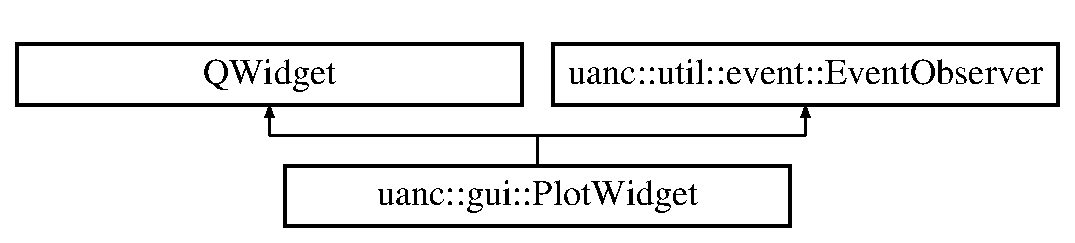
\includegraphics[height=2.000000cm]{classuanc_1_1gui_1_1_plot_widget}
\end{center}
\end{figure}
\subsection*{Public Slots}
\begin{DoxyCompactItemize}
\item 
void \hyperlink{classuanc_1_1gui_1_1_plot_widget_ac9bd837545242bbe1f9e0b5ca6b6a40a}{save\+Signal} ()
\begin{DoxyCompactList}\small\item\em saves the signal to the fileactor \end{DoxyCompactList}\end{DoxyCompactItemize}
\subsection*{Public Member Functions}
\begin{DoxyCompactItemize}
\item 
\hyperlink{classuanc_1_1gui_1_1_plot_widget_af448f772ff5abbe5786a7fa0a448e217}{Plot\+Widget} ()
\item 
void \hyperlink{classuanc_1_1gui_1_1_plot_widget_a66a5565461bcb900c4d7003f75781e62}{set\+Signal} (std\+::shared\+\_\+ptr$<$ \hyperlink{classuanc_1_1amv_1_1_inverted_model}{uanc\+::amv\+::\+Inverted\+Model} $>$ \hyperlink{classuanc_1_1gui_1_1_plot_widget_a2c7050da7a3c85ce55cb95ffd1dc2eb8}{signal})
\begin{DoxyCompactList}\small\item\em This method is for setting a Signal. This method is for setting a Signal. The Signal will immediately be plotted. \end{DoxyCompactList}\item 
void \hyperlink{classuanc_1_1gui_1_1_plot_widget_a15f259c15b2db5c26f9181f8a8fca705}{set\+Centered\+Y\+Axis} (bool b)
\begin{DoxyCompactList}\small\item\em This method is for setting the Y\+Axis This method is for setting the Y\+Axis to true or false. \end{DoxyCompactList}\item 
const Q\+C\+P\+Range \hyperlink{classuanc_1_1gui_1_1_plot_widget_add4f78d4efad5b7f27caae2535620e56}{get\+Plot\+X\+Range} () const 
\begin{DoxyCompactList}\small\item\em Returns the current range of the x axis of the plot. \end{DoxyCompactList}\item 
void \hyperlink{classuanc_1_1gui_1_1_plot_widget_a8a2eb029622ad4ec3ee100f9bcc68732}{plot\+Changed} ()
\begin{DoxyCompactList}\small\item\em This method is for triggering the control to update because the plot changed. \end{DoxyCompactList}\item 
void \hyperlink{classuanc_1_1gui_1_1_plot_widget_a9db10479dc8c6590713a18e5a2607138}{control\+Changed} ()
\begin{DoxyCompactList}\small\item\em This method is for triggering the plot to update because the state of the control changed. \end{DoxyCompactList}\item 
std\+::shared\+\_\+ptr$<$ \hyperlink{classuanc_1_1amv_1_1_signal_model}{uanc\+::amv\+::\+Signal\+Model} $>$ \hyperlink{classuanc_1_1gui_1_1_plot_widget_a2c7050da7a3c85ce55cb95ffd1dc2eb8}{signal} ()
\begin{DoxyCompactList}\small\item\em Constructor for signals. \end{DoxyCompactList}\item 
std\+::shared\+\_\+ptr$<$ \hyperlink{classuanc_1_1amv_1_1_signal_model}{uanc\+::amv\+::\+Signal\+Model} $>$ \hyperlink{classuanc_1_1gui_1_1_plot_widget_a9a678b758c7ebf06680ed190badcfe36}{error\+Signal} ()
\begin{DoxyCompactList}\small\item\em simply returns the error signal \end{DoxyCompactList}\item 
double \hyperlink{classuanc_1_1gui_1_1_plot_widget_ab89e84ccfbc81bc77fef0fd9301273a3}{last\+Index} ()
\begin{DoxyCompactList}\small\item\em simple returns the the last index \end{DoxyCompactList}\end{DoxyCompactItemize}
\subsection*{Additional Inherited Members}


\subsection{Constructor \& Destructor Documentation}
\index{uanc\+::gui\+::\+Plot\+Widget@{uanc\+::gui\+::\+Plot\+Widget}!Plot\+Widget@{Plot\+Widget}}
\index{Plot\+Widget@{Plot\+Widget}!uanc\+::gui\+::\+Plot\+Widget@{uanc\+::gui\+::\+Plot\+Widget}}
\subsubsection[{\texorpdfstring{Plot\+Widget()}{PlotWidget()}}]{\setlength{\rightskip}{0pt plus 5cm}uanc\+::gui\+::\+Plot\+Widget\+::\+Plot\+Widget (
\begin{DoxyParamCaption}
{}
\end{DoxyParamCaption}
)}\hypertarget{classuanc_1_1gui_1_1_plot_widget_af448f772ff5abbe5786a7fa0a448e217}{}\label{classuanc_1_1gui_1_1_plot_widget_af448f772ff5abbe5786a7fa0a448e217}
Contructor 

\subsection{Member Function Documentation}
\index{uanc\+::gui\+::\+Plot\+Widget@{uanc\+::gui\+::\+Plot\+Widget}!control\+Changed@{control\+Changed}}
\index{control\+Changed@{control\+Changed}!uanc\+::gui\+::\+Plot\+Widget@{uanc\+::gui\+::\+Plot\+Widget}}
\subsubsection[{\texorpdfstring{control\+Changed()}{controlChanged()}}]{\setlength{\rightskip}{0pt plus 5cm}void uanc\+::gui\+::\+Plot\+Widget\+::control\+Changed (
\begin{DoxyParamCaption}
{}
\end{DoxyParamCaption}
)}\hypertarget{classuanc_1_1gui_1_1_plot_widget_a9db10479dc8c6590713a18e5a2607138}{}\label{classuanc_1_1gui_1_1_plot_widget_a9db10479dc8c6590713a18e5a2607138}


This method is for triggering the plot to update because the state of the control changed. 

\index{uanc\+::gui\+::\+Plot\+Widget@{uanc\+::gui\+::\+Plot\+Widget}!error\+Signal@{error\+Signal}}
\index{error\+Signal@{error\+Signal}!uanc\+::gui\+::\+Plot\+Widget@{uanc\+::gui\+::\+Plot\+Widget}}
\subsubsection[{\texorpdfstring{error\+Signal()}{errorSignal()}}]{\setlength{\rightskip}{0pt plus 5cm}std\+::shared\+\_\+ptr$<${\bf uanc\+::amv\+::\+Signal\+Model}$>$ uanc\+::gui\+::\+Plot\+Widget\+::error\+Signal (
\begin{DoxyParamCaption}
{}
\end{DoxyParamCaption}
)\hspace{0.3cm}{\ttfamily [inline]}}\hypertarget{classuanc_1_1gui_1_1_plot_widget_a9a678b758c7ebf06680ed190badcfe36}{}\label{classuanc_1_1gui_1_1_plot_widget_a9a678b758c7ebf06680ed190badcfe36}


simply returns the error signal 

\begin{DoxyReturn}{Returns}
a Signal\+Model of the error signal 
\end{DoxyReturn}
\index{uanc\+::gui\+::\+Plot\+Widget@{uanc\+::gui\+::\+Plot\+Widget}!get\+Plot\+X\+Range@{get\+Plot\+X\+Range}}
\index{get\+Plot\+X\+Range@{get\+Plot\+X\+Range}!uanc\+::gui\+::\+Plot\+Widget@{uanc\+::gui\+::\+Plot\+Widget}}
\subsubsection[{\texorpdfstring{get\+Plot\+X\+Range() const }{getPlotXRange() const }}]{\setlength{\rightskip}{0pt plus 5cm}const Q\+C\+P\+Range uanc\+::gui\+::\+Plot\+Widget\+::get\+Plot\+X\+Range (
\begin{DoxyParamCaption}
{}
\end{DoxyParamCaption}
) const}\hypertarget{classuanc_1_1gui_1_1_plot_widget_add4f78d4efad5b7f27caae2535620e56}{}\label{classuanc_1_1gui_1_1_plot_widget_add4f78d4efad5b7f27caae2535620e56}


Returns the current range of the x axis of the plot. 

\begin{DoxyReturn}{Returns}
Current range of the x axis of the plot. 
\end{DoxyReturn}
\index{uanc\+::gui\+::\+Plot\+Widget@{uanc\+::gui\+::\+Plot\+Widget}!last\+Index@{last\+Index}}
\index{last\+Index@{last\+Index}!uanc\+::gui\+::\+Plot\+Widget@{uanc\+::gui\+::\+Plot\+Widget}}
\subsubsection[{\texorpdfstring{last\+Index()}{lastIndex()}}]{\setlength{\rightskip}{0pt plus 5cm}double uanc\+::gui\+::\+Plot\+Widget\+::last\+Index (
\begin{DoxyParamCaption}
{}
\end{DoxyParamCaption}
)\hspace{0.3cm}{\ttfamily [inline]}}\hypertarget{classuanc_1_1gui_1_1_plot_widget_ab89e84ccfbc81bc77fef0fd9301273a3}{}\label{classuanc_1_1gui_1_1_plot_widget_ab89e84ccfbc81bc77fef0fd9301273a3}


simple returns the the last index 

\begin{DoxyReturn}{Returns}
a double with the last index 
\end{DoxyReturn}
\index{uanc\+::gui\+::\+Plot\+Widget@{uanc\+::gui\+::\+Plot\+Widget}!plot\+Changed@{plot\+Changed}}
\index{plot\+Changed@{plot\+Changed}!uanc\+::gui\+::\+Plot\+Widget@{uanc\+::gui\+::\+Plot\+Widget}}
\subsubsection[{\texorpdfstring{plot\+Changed()}{plotChanged()}}]{\setlength{\rightskip}{0pt plus 5cm}void uanc\+::gui\+::\+Plot\+Widget\+::plot\+Changed (
\begin{DoxyParamCaption}
{}
\end{DoxyParamCaption}
)}\hypertarget{classuanc_1_1gui_1_1_plot_widget_a8a2eb029622ad4ec3ee100f9bcc68732}{}\label{classuanc_1_1gui_1_1_plot_widget_a8a2eb029622ad4ec3ee100f9bcc68732}


This method is for triggering the control to update because the plot changed. 

\index{uanc\+::gui\+::\+Plot\+Widget@{uanc\+::gui\+::\+Plot\+Widget}!save\+Signal@{save\+Signal}}
\index{save\+Signal@{save\+Signal}!uanc\+::gui\+::\+Plot\+Widget@{uanc\+::gui\+::\+Plot\+Widget}}
\subsubsection[{\texorpdfstring{save\+Signal}{saveSignal}}]{\setlength{\rightskip}{0pt plus 5cm}void uanc\+::gui\+::\+Plot\+Widget\+::save\+Signal (
\begin{DoxyParamCaption}
{}
\end{DoxyParamCaption}
)\hspace{0.3cm}{\ttfamily [slot]}}\hypertarget{classuanc_1_1gui_1_1_plot_widget_ac9bd837545242bbe1f9e0b5ca6b6a40a}{}\label{classuanc_1_1gui_1_1_plot_widget_ac9bd837545242bbe1f9e0b5ca6b6a40a}


saves the signal to the fileactor 

\index{uanc\+::gui\+::\+Plot\+Widget@{uanc\+::gui\+::\+Plot\+Widget}!set\+Centered\+Y\+Axis@{set\+Centered\+Y\+Axis}}
\index{set\+Centered\+Y\+Axis@{set\+Centered\+Y\+Axis}!uanc\+::gui\+::\+Plot\+Widget@{uanc\+::gui\+::\+Plot\+Widget}}
\subsubsection[{\texorpdfstring{set\+Centered\+Y\+Axis(bool b)}{setCenteredYAxis(bool b)}}]{\setlength{\rightskip}{0pt plus 5cm}void uanc\+::gui\+::\+Plot\+Widget\+::set\+Centered\+Y\+Axis (
\begin{DoxyParamCaption}
\item[{bool}]{b}
\end{DoxyParamCaption}
)\hspace{0.3cm}{\ttfamily [inline]}}\hypertarget{classuanc_1_1gui_1_1_plot_widget_a15f259c15b2db5c26f9181f8a8fca705}{}\label{classuanc_1_1gui_1_1_plot_widget_a15f259c15b2db5c26f9181f8a8fca705}


This method is for setting the Y\+Axis This method is for setting the Y\+Axis to true or false. 


\begin{DoxyParams}{Parameters}
{\em b} & given boolean \\
\hline
\end{DoxyParams}
\index{uanc\+::gui\+::\+Plot\+Widget@{uanc\+::gui\+::\+Plot\+Widget}!set\+Signal@{set\+Signal}}
\index{set\+Signal@{set\+Signal}!uanc\+::gui\+::\+Plot\+Widget@{uanc\+::gui\+::\+Plot\+Widget}}
\subsubsection[{\texorpdfstring{set\+Signal(std\+::shared\+\_\+ptr$<$ uanc\+::amv\+::\+Inverted\+Model $>$ signal)}{setSignal(std::shared_ptr< uanc::amv::InvertedModel > signal)}}]{\setlength{\rightskip}{0pt plus 5cm}void uanc\+::gui\+::\+Plot\+Widget\+::set\+Signal (
\begin{DoxyParamCaption}
\item[{std\+::shared\+\_\+ptr$<$ {\bf uanc\+::amv\+::\+Inverted\+Model} $>$}]{signal}
\end{DoxyParamCaption}
)}\hypertarget{classuanc_1_1gui_1_1_plot_widget_a66a5565461bcb900c4d7003f75781e62}{}\label{classuanc_1_1gui_1_1_plot_widget_a66a5565461bcb900c4d7003f75781e62}


This method is for setting a Signal. This method is for setting a Signal. The Signal will immediately be plotted. 


\begin{DoxyParams}{Parameters}
{\em signal} & The Aquila\+::\+Signal\+Source which will be plotted \\
\hline
\end{DoxyParams}
\index{uanc\+::gui\+::\+Plot\+Widget@{uanc\+::gui\+::\+Plot\+Widget}!signal@{signal}}
\index{signal@{signal}!uanc\+::gui\+::\+Plot\+Widget@{uanc\+::gui\+::\+Plot\+Widget}}
\subsubsection[{\texorpdfstring{signal()}{signal()}}]{\setlength{\rightskip}{0pt plus 5cm}std\+::shared\+\_\+ptr$<${\bf uanc\+::amv\+::\+Signal\+Model}$>$ uanc\+::gui\+::\+Plot\+Widget\+::signal (
\begin{DoxyParamCaption}
{}
\end{DoxyParamCaption}
)\hspace{0.3cm}{\ttfamily [inline]}}\hypertarget{classuanc_1_1gui_1_1_plot_widget_a2c7050da7a3c85ce55cb95ffd1dc2eb8}{}\label{classuanc_1_1gui_1_1_plot_widget_a2c7050da7a3c85ce55cb95ffd1dc2eb8}


Constructor for signals. 

\begin{DoxyReturn}{Returns}
a Signal\+Model 
\end{DoxyReturn}


The documentation for this class was generated from the following files\+:\begin{DoxyCompactItemize}
\item 
/home/kurt/\+Documents/\+Studium/\+Bachelor\+\_\+\+Praktikum/\+U\+A\+N\+C/\+Code/\+U\+A\+N\+C/gui/\hyperlink{_plot_widget_8h}{Plot\+Widget.\+h}\item 
/home/kurt/\+Documents/\+Studium/\+Bachelor\+\_\+\+Praktikum/\+U\+A\+N\+C/\+Code/\+U\+A\+N\+C/gui/\hyperlink{_plot_widget_8cpp}{Plot\+Widget.\+cpp}\end{DoxyCompactItemize}

\hypertarget{classuanc_1_1amv_1_1anc_1_1view_1_1_p_m_view}{}\section{uanc\+:\+:amv\+:\+:anc\+:\+:view\+:\+:P\+M\+View Class Reference}
\label{classuanc_1_1amv_1_1anc_1_1view_1_1_p_m_view}\index{uanc\+::amv\+::anc\+::view\+::\+P\+M\+View@{uanc\+::amv\+::anc\+::view\+::\+P\+M\+View}}


Represents an \hyperlink{classuanc_1_1amv_1_1anc_1_1view_1_1_p_m_view}{P\+M\+View}.  




{\ttfamily \#include $<$P\+M\+View.\+h$>$}

Inheritance diagram for uanc\+:\+:amv\+:\+:anc\+:\+:view\+:\+:P\+M\+View\+:\begin{figure}[H]
\begin{center}
\leavevmode
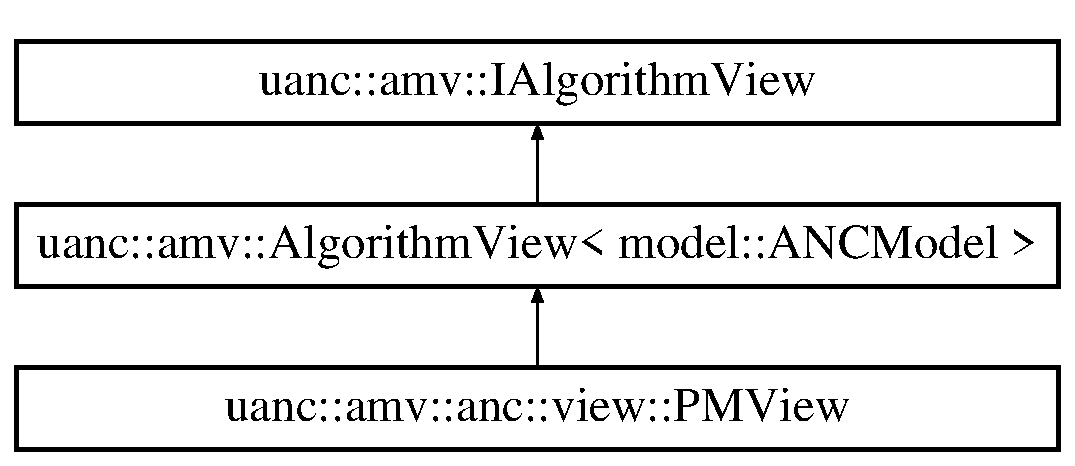
\includegraphics[height=3.000000cm]{classuanc_1_1amv_1_1anc_1_1view_1_1_p_m_view}
\end{center}
\end{figure}
\subsection*{Public Member Functions}
\begin{DoxyCompactItemize}
\item 
Q\+Widget $\ast$ \hyperlink{classuanc_1_1amv_1_1anc_1_1view_1_1_p_m_view_a4f4d6f52427201d7dcd671c7932824ad}{produce\+Widget} () final
\begin{DoxyCompactList}\small\item\em Gets the complete widget. \end{DoxyCompactList}\item 
void \hyperlink{classuanc_1_1amv_1_1anc_1_1view_1_1_p_m_view_a6d87a1d7753d1bc76ac7fba5fa03e1d5}{set\+Data} (std\+::shared\+\_\+ptr$<$ \hyperlink{classuanc_1_1amv_1_1anc_1_1model_1_1_a_n_c_model}{model\+::\+A\+N\+C\+Model} $>$ signal\+Data) final
\begin{DoxyCompactList}\small\item\em This method applies the model data. \end{DoxyCompactList}\end{DoxyCompactItemize}


\subsection{Detailed Description}
Represents an \hyperlink{classuanc_1_1amv_1_1anc_1_1view_1_1_p_m_view}{P\+M\+View}. 

This represents a general \hyperlink{classuanc_1_1amv_1_1anc_1_1view_1_1_p_m_view}{P\+M\+View}. It operates on an A\+N\+C\+Model and P\+M\+Model. It displays a simple plot of the the inverted signal and performance informations of the algorithm. It is a specialization of the more general \hyperlink{classuanc_1_1amv_1_1_algorithm_view}{Algorithm\+View}. 

\subsection{Member Function Documentation}
\index{uanc\+::amv\+::anc\+::view\+::\+P\+M\+View@{uanc\+::amv\+::anc\+::view\+::\+P\+M\+View}!produce\+Widget@{produce\+Widget}}
\index{produce\+Widget@{produce\+Widget}!uanc\+::amv\+::anc\+::view\+::\+P\+M\+View@{uanc\+::amv\+::anc\+::view\+::\+P\+M\+View}}
\subsubsection[{\texorpdfstring{produce\+Widget() final}{produceWidget() final}}]{\setlength{\rightskip}{0pt plus 5cm}Q\+Widget $\ast$ uanc\+::amv\+::anc\+::view\+::\+P\+M\+View\+::produce\+Widget (
\begin{DoxyParamCaption}
{}
\end{DoxyParamCaption}
)\hspace{0.3cm}{\ttfamily [final]}, {\ttfamily [virtual]}}\hypertarget{classuanc_1_1amv_1_1anc_1_1view_1_1_p_m_view_a4f4d6f52427201d7dcd671c7932824ad}{}\label{classuanc_1_1amv_1_1anc_1_1view_1_1_p_m_view_a4f4d6f52427201d7dcd671c7932824ad}


Gets the complete widget. 

This function is used to retrieve the widget from the view. It gets used for integration the main application. It holds a Plotwidget and a Tree\+View inside of a Q\+Widget (horizontal layout) and passes this back.

\begin{DoxyReturn}{Returns}
The created widget.
\end{DoxyReturn}
This function is used to retrieve the widget from the view. It gets used for integration the main application. It creates a Plotwidget inside of a Q\+Widget and passes this back. Uses the singleton pattern to ensure the unique creation of the widget.

\begin{DoxyReturn}{Returns}
The created widget. 
\end{DoxyReturn}


Implements \hyperlink{classuanc_1_1amv_1_1_i_algorithm_view_ab9d06a0b43db57244868f10dae8e09e5}{uanc\+::amv\+::\+I\+Algorithm\+View}.

\index{uanc\+::amv\+::anc\+::view\+::\+P\+M\+View@{uanc\+::amv\+::anc\+::view\+::\+P\+M\+View}!set\+Data@{set\+Data}}
\index{set\+Data@{set\+Data}!uanc\+::amv\+::anc\+::view\+::\+P\+M\+View@{uanc\+::amv\+::anc\+::view\+::\+P\+M\+View}}
\subsubsection[{\texorpdfstring{set\+Data(std\+::shared\+\_\+ptr$<$ model\+::\+A\+N\+C\+Model $>$ signal\+Data) final}{setData(std::shared_ptr< model::ANCModel > signalData) final}}]{\setlength{\rightskip}{0pt plus 5cm}void uanc\+::amv\+::anc\+::view\+::\+P\+M\+View\+::set\+Data (
\begin{DoxyParamCaption}
\item[{std\+::shared\+\_\+ptr$<$ {\bf model\+::\+A\+N\+C\+Model} $>$}]{signal\+Data}
\end{DoxyParamCaption}
)\hspace{0.3cm}{\ttfamily [final]}, {\ttfamily [virtual]}}\hypertarget{classuanc_1_1amv_1_1anc_1_1view_1_1_p_m_view_a6d87a1d7753d1bc76ac7fba5fa03e1d5}{}\label{classuanc_1_1amv_1_1anc_1_1view_1_1_p_m_view_a6d87a1d7753d1bc76ac7fba5fa03e1d5}


This method applies the model data. 

This method simply takes the passed data and places it inside of the view at the appropriate places.


\begin{DoxyParams}{Parameters}
{\em data} & The applied data. \\
\hline
\end{DoxyParams}


Implements \hyperlink{classuanc_1_1amv_1_1_algorithm_view_ad656cf5223a66a942441ee39f44f65a3}{uanc\+::amv\+::\+Algorithm\+View$<$ model\+::\+A\+N\+C\+Model $>$}.



The documentation for this class was generated from the following files\+:\begin{DoxyCompactItemize}
\item 
/home/kurt/\+Documents/\+Studium/\+Bachelor\+\_\+\+Praktikum/\+U\+A\+N\+C/\+Code/\+U\+A\+N\+C/amv/anc/view/\hyperlink{_p_m_view_8h}{P\+M\+View.\+h}\item 
/home/kurt/\+Documents/\+Studium/\+Bachelor\+\_\+\+Praktikum/\+U\+A\+N\+C/\+Code/\+U\+A\+N\+C/amv/anc/view/\hyperlink{_p_m_view_8cpp}{P\+M\+View.\+cpp}\end{DoxyCompactItemize}

\hypertarget{classuanc_1_1gui_1_1_p_m_widget}{}\section{uanc\+:\+:gui\+:\+:P\+M\+Widget Class Reference}
\label{classuanc_1_1gui_1_1_p_m_widget}\index{uanc\+::gui\+::\+P\+M\+Widget@{uanc\+::gui\+::\+P\+M\+Widget}}


{\ttfamily \#include $<$P\+M\+Widget.\+h$>$}

Inheritance diagram for uanc\+:\+:gui\+:\+:P\+M\+Widget\+:\begin{figure}[H]
\begin{center}
\leavevmode
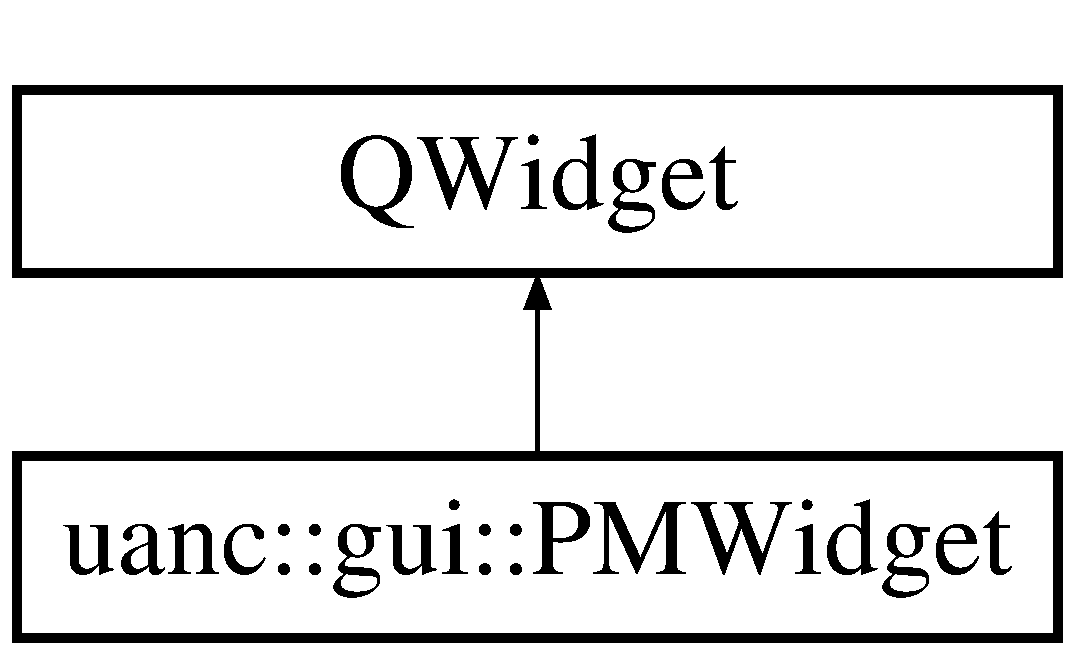
\includegraphics[height=2.000000cm]{classuanc_1_1gui_1_1_p_m_widget}
\end{center}
\end{figure}
\subsection*{Public Slots}
\begin{DoxyCompactItemize}
\item 
void \hyperlink{classuanc_1_1gui_1_1_p_m_widget_a308f665936b00c8f0b84174756ffbc5b}{toogle\+Performance} ()
\begin{DoxyCompactList}\small\item\em simple hides or shows the performance measurement \end{DoxyCompactList}\end{DoxyCompactItemize}
\subsection*{Public Member Functions}
\begin{DoxyCompactItemize}
\item 
\hyperlink{classuanc_1_1gui_1_1_p_m_widget_a0b42fd60ea9465083fa8b62189b23092}{P\+M\+Widget} ()
\item 
void \hyperlink{classuanc_1_1gui_1_1_p_m_widget_a072fa5f18b164d05a51407c088bf2ffb}{set\+Data} (std\+::vector$<$ std\+::shared\+\_\+ptr$<$ \hyperlink{classuanc_1_1util_1_1_performance_measure}{uanc\+::util\+::\+Performance\+Measure}$<$$>$$>$$>$ performance\+Data)
\begin{DoxyCompactList}\small\item\em This method is for setting the measurement information. This method is for setting the measurement information. \end{DoxyCompactList}\end{DoxyCompactItemize}


\subsection{Constructor \& Destructor Documentation}
\index{uanc\+::gui\+::\+P\+M\+Widget@{uanc\+::gui\+::\+P\+M\+Widget}!P\+M\+Widget@{P\+M\+Widget}}
\index{P\+M\+Widget@{P\+M\+Widget}!uanc\+::gui\+::\+P\+M\+Widget@{uanc\+::gui\+::\+P\+M\+Widget}}
\subsubsection[{\texorpdfstring{P\+M\+Widget()}{PMWidget()}}]{\setlength{\rightskip}{0pt plus 5cm}uanc\+::gui\+::\+P\+M\+Widget\+::\+P\+M\+Widget (
\begin{DoxyParamCaption}
{}
\end{DoxyParamCaption}
)}\hypertarget{classuanc_1_1gui_1_1_p_m_widget_a0b42fd60ea9465083fa8b62189b23092}{}\label{classuanc_1_1gui_1_1_p_m_widget_a0b42fd60ea9465083fa8b62189b23092}
Contructor 

\subsection{Member Function Documentation}
\index{uanc\+::gui\+::\+P\+M\+Widget@{uanc\+::gui\+::\+P\+M\+Widget}!set\+Data@{set\+Data}}
\index{set\+Data@{set\+Data}!uanc\+::gui\+::\+P\+M\+Widget@{uanc\+::gui\+::\+P\+M\+Widget}}
\subsubsection[{\texorpdfstring{set\+Data(std\+::vector$<$ std\+::shared\+\_\+ptr$<$ uanc\+::util\+::\+Performance\+Measure$<$$>$$>$$>$ performance\+Data)}{setData(std::vector< std::shared_ptr< uanc::util::PerformanceMeasure<>>> performanceData)}}]{\setlength{\rightskip}{0pt plus 5cm}void uanc\+::gui\+::\+P\+M\+Widget\+::set\+Data (
\begin{DoxyParamCaption}
\item[{std\+::vector$<$ std\+::shared\+\_\+ptr$<$ {\bf uanc\+::util\+::\+Performance\+Measure}$<$$>$$>$$>$}]{performance\+Data}
\end{DoxyParamCaption}
)}\hypertarget{classuanc_1_1gui_1_1_p_m_widget_a072fa5f18b164d05a51407c088bf2ffb}{}\label{classuanc_1_1gui_1_1_p_m_widget_a072fa5f18b164d05a51407c088bf2ffb}


This method is for setting the measurement information. This method is for setting the measurement information. 


\begin{DoxyParams}{Parameters}
{\em signal} & The Aquila\+::\+Signal\+Source which will be plotted \\
\hline
\end{DoxyParams}
\index{uanc\+::gui\+::\+P\+M\+Widget@{uanc\+::gui\+::\+P\+M\+Widget}!toogle\+Performance@{toogle\+Performance}}
\index{toogle\+Performance@{toogle\+Performance}!uanc\+::gui\+::\+P\+M\+Widget@{uanc\+::gui\+::\+P\+M\+Widget}}
\subsubsection[{\texorpdfstring{toogle\+Performance}{tooglePerformance}}]{\setlength{\rightskip}{0pt plus 5cm}void uanc\+::gui\+::\+P\+M\+Widget\+::toogle\+Performance (
\begin{DoxyParamCaption}
{}
\end{DoxyParamCaption}
)\hspace{0.3cm}{\ttfamily [slot]}}\hypertarget{classuanc_1_1gui_1_1_p_m_widget_a308f665936b00c8f0b84174756ffbc5b}{}\label{classuanc_1_1gui_1_1_p_m_widget_a308f665936b00c8f0b84174756ffbc5b}


simple hides or shows the performance measurement 



The documentation for this class was generated from the following files\+:\begin{DoxyCompactItemize}
\item 
/ext/local/\+University/\+B\+P/\+Git/\+U\+A\+N\+C/\+Code/\+U\+A\+N\+C/gui/\hyperlink{_p_m_widget_8h}{P\+M\+Widget.\+h}\item 
/ext/local/\+University/\+B\+P/\+Git/\+U\+A\+N\+C/\+Code/\+U\+A\+N\+C/gui/\hyperlink{_p_m_widget_8cpp}{P\+M\+Widget.\+cpp}\end{DoxyCompactItemize}

\hypertarget{classuanc_1_1util_1_1_signal_file_actor}{}\section{uanc\+:\+:util\+:\+:Signal\+File\+Actor Class Reference}
\label{classuanc_1_1util_1_1_signal_file_actor}\index{uanc\+::util\+::\+Signal\+File\+Actor@{uanc\+::util\+::\+Signal\+File\+Actor}}


Basic Signal file loader class.  




{\ttfamily \#include $<$Signal\+File\+Actor.\+h$>$}

Inheritance diagram for uanc\+:\+:util\+:\+:Signal\+File\+Actor\+:\begin{figure}[H]
\begin{center}
\leavevmode
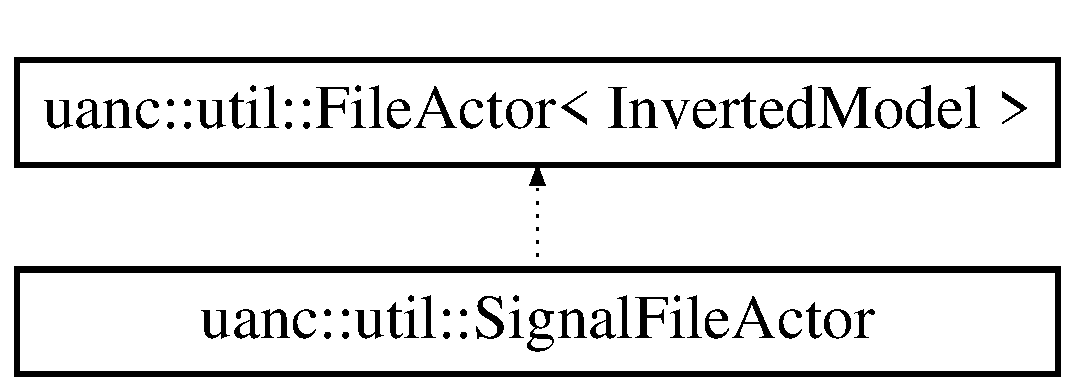
\includegraphics[height=2.000000cm]{classuanc_1_1util_1_1_signal_file_actor}
\end{center}
\end{figure}
\subsection*{Public Member Functions}
\begin{DoxyCompactItemize}
\item 
\hyperlink{classuanc_1_1util_1_1_signal_file_actor_a0c4e494e7e700d4e0130b56e4dc82b8f}{Signal\+File\+Actor} (const std\+::string \&path)
\begin{DoxyCompactList}\small\item\em Basic constructor which saves a path string internally. \end{DoxyCompactList}\item 
std\+::shared\+\_\+ptr$<$ \hyperlink{classuanc_1_1amv_1_1_inverted_model}{Inverted\+Model} $>$ \hyperlink{classuanc_1_1util_1_1_signal_file_actor_a2069e33e03ebc63eac2080d40f863ce3}{load\+Data} ()
\begin{DoxyCompactList}\small\item\em This method should load the file from the plate. \end{DoxyCompactList}\item 
void \hyperlink{classuanc_1_1util_1_1_signal_file_actor_a77695bd57923ec24ff78ec8361bcfca2}{save\+Data} (std\+::shared\+\_\+ptr$<$ \hyperlink{classuanc_1_1amv_1_1_inverted_model}{Inverted\+Model} $>$ source)
\begin{DoxyCompactList}\small\item\em This method should save a file to the plate. \end{DoxyCompactList}\end{DoxyCompactItemize}


\subsection{Detailed Description}
Basic Signal file loader class. 

Is derived from the file loader class itself. 

\subsection{Constructor \& Destructor Documentation}
\index{uanc\+::util\+::\+Signal\+File\+Actor@{uanc\+::util\+::\+Signal\+File\+Actor}!Signal\+File\+Actor@{Signal\+File\+Actor}}
\index{Signal\+File\+Actor@{Signal\+File\+Actor}!uanc\+::util\+::\+Signal\+File\+Actor@{uanc\+::util\+::\+Signal\+File\+Actor}}
\subsubsection[{\texorpdfstring{Signal\+File\+Actor(const std\+::string \&path)}{SignalFileActor(const std::string &path)}}]{\setlength{\rightskip}{0pt plus 5cm}uanc\+::util\+::\+Signal\+File\+Actor\+::\+Signal\+File\+Actor (
\begin{DoxyParamCaption}
\item[{const std\+::string \&}]{path}
\end{DoxyParamCaption}
)\hspace{0.3cm}{\ttfamily [inline]}}\hypertarget{classuanc_1_1util_1_1_signal_file_actor_a0c4e494e7e700d4e0130b56e4dc82b8f}{}\label{classuanc_1_1util_1_1_signal_file_actor_a0c4e494e7e700d4e0130b56e4dc82b8f}


Basic constructor which saves a path string internally. 

This constructor just save the passed string internally.


\begin{DoxyParams}{Parameters}
{\em path} & The path to the acted file \\
\hline
\end{DoxyParams}


\subsection{Member Function Documentation}
\index{uanc\+::util\+::\+Signal\+File\+Actor@{uanc\+::util\+::\+Signal\+File\+Actor}!load\+Data@{load\+Data}}
\index{load\+Data@{load\+Data}!uanc\+::util\+::\+Signal\+File\+Actor@{uanc\+::util\+::\+Signal\+File\+Actor}}
\subsubsection[{\texorpdfstring{load\+Data()}{loadData()}}]{\setlength{\rightskip}{0pt plus 5cm}std\+::shared\+\_\+ptr$<${\bf Inverted\+Model}$>$ uanc\+::util\+::\+Signal\+File\+Actor\+::load\+Data (
\begin{DoxyParamCaption}
{}
\end{DoxyParamCaption}
)\hspace{0.3cm}{\ttfamily [inline]}, {\ttfamily [virtual]}}\hypertarget{classuanc_1_1util_1_1_signal_file_actor_a2069e33e03ebc63eac2080d40f863ce3}{}\label{classuanc_1_1util_1_1_signal_file_actor_a2069e33e03ebc63eac2080d40f863ce3}


This method should load the file from the plate. 

This method should return the loaded T

\begin{DoxyReturn}{Returns}
the loaded T 
\end{DoxyReturn}


Implements \hyperlink{classuanc_1_1util_1_1_file_actor_ad2db7584c9332a4d8376ccf6276ec301}{uanc\+::util\+::\+File\+Actor$<$ Inverted\+Model $>$}.

\index{uanc\+::util\+::\+Signal\+File\+Actor@{uanc\+::util\+::\+Signal\+File\+Actor}!save\+Data@{save\+Data}}
\index{save\+Data@{save\+Data}!uanc\+::util\+::\+Signal\+File\+Actor@{uanc\+::util\+::\+Signal\+File\+Actor}}
\subsubsection[{\texorpdfstring{save\+Data(std\+::shared\+\_\+ptr$<$ Inverted\+Model $>$ source)}{saveData(std::shared_ptr< InvertedModel > source)}}]{\setlength{\rightskip}{0pt plus 5cm}void uanc\+::util\+::\+Signal\+File\+Actor\+::save\+Data (
\begin{DoxyParamCaption}
\item[{std\+::shared\+\_\+ptr$<$ {\bf Inverted\+Model} $>$}]{source}
\end{DoxyParamCaption}
)\hspace{0.3cm}{\ttfamily [inline]}, {\ttfamily [virtual]}}\hypertarget{classuanc_1_1util_1_1_signal_file_actor_a77695bd57923ec24ff78ec8361bcfca2}{}\label{classuanc_1_1util_1_1_signal_file_actor_a77695bd57923ec24ff78ec8361bcfca2}


This method should save a file to the plate. 

This should method should save the passed T to the specified path.


\begin{DoxyParams}{Parameters}
{\em source} & The source to save \\
\hline
\end{DoxyParams}


Implements \hyperlink{classuanc_1_1util_1_1_file_actor_aee5e36b37c46dda87f0499fc7b9e4b0d}{uanc\+::util\+::\+File\+Actor$<$ Inverted\+Model $>$}.



The documentation for this class was generated from the following file\+:\begin{DoxyCompactItemize}
\item 
/home/kurt/\+Documents/\+Studium/\+Bachelor\+\_\+\+Praktikum/\+U\+A\+N\+C/\+Code/\+U\+A\+N\+C/util/\hyperlink{_signal_file_actor_8h}{Signal\+File\+Actor.\+h}\end{DoxyCompactItemize}

\hypertarget{classuanc_1_1util_1_1_signal_manager}{}\section{uanc\+:\+:util\+:\+:Signal\+Manager Class Reference}
\label{classuanc_1_1util_1_1_signal_manager}\index{uanc\+::util\+::\+Signal\+Manager@{uanc\+::util\+::\+Signal\+Manager}}


{\ttfamily \#include $<$Signal\+Manager.\+h$>$}

\subsection*{Public Member Functions}
\begin{DoxyCompactItemize}
\item 
\hyperlink{classuanc_1_1util_1_1_signal_manager_abc5fe781a15e9f7dfd5976055101421d}{Signal\+Manager} ()
\begin{DoxyCompactList}\small\item\em Private constructor to deny creation outside of the singleton pattern. \end{DoxyCompactList}\item 
int \hyperlink{classuanc_1_1util_1_1_signal_manager_a23ca36b1dc644f2bdb218c95aa548a22}{add\+Signal} (const \hyperlink{classuanc_1_1amv_1_1_inverted_model}{Inverted\+Model} \&signal\+Source)
\begin{DoxyCompactList}\small\item\em Adds a signal to the internal map. \end{DoxyCompactList}\item 
int \hyperlink{classuanc_1_1util_1_1_signal_manager_a2e78bbe03560797e5f8d289fad36aa9f}{add\+Signal} (std\+::shared\+\_\+ptr$<$ \hyperlink{classuanc_1_1amv_1_1_inverted_model}{Inverted\+Model} $>$ signal\+Source)
\begin{DoxyCompactList}\small\item\em Adds a signal to the internal map. \end{DoxyCompactList}\item 
std\+::shared\+\_\+ptr$<$ \hyperlink{classuanc_1_1amv_1_1_inverted_model}{Inverted\+Model} $>$ \hyperlink{classuanc_1_1util_1_1_signal_manager_a57b20729a18cf0b1c119a4fe6eef398a}{get\+Signal} (int name)
\begin{DoxyCompactList}\small\item\em This method returns a signal as a weak ptr. \end{DoxyCompactList}\item 
void \hyperlink{classuanc_1_1util_1_1_signal_manager_a26920917057ae9c917703a1143d832ca}{erase\+Signal} (int index)
\begin{DoxyCompactList}\small\item\em This method deletes a signal. \end{DoxyCompactList}\end{DoxyCompactItemize}
\subsection*{Static Public Member Functions}
\begin{DoxyCompactItemize}
\item 
static std\+::shared\+\_\+ptr$<$ \hyperlink{classuanc_1_1util_1_1_signal_manager}{Signal\+Manager} $>$ \hyperlink{classuanc_1_1util_1_1_signal_manager_a95eace0493a19f4e9470b6e353b9fe68}{get} ()
\begin{DoxyCompactList}\small\item\em Obtain a reference to the main window. \end{DoxyCompactList}\end{DoxyCompactItemize}
\subsection*{Public Attributes}
\begin{DoxyCompactItemize}
\item 
int \hyperlink{classuanc_1_1util_1_1_signal_manager_a8f433e771d5933242b75e35397078ecb}{signal\+Counter} = -\/1
\end{DoxyCompactItemize}
\subsection*{Static Public Attributes}
\begin{DoxyCompactItemize}
\item 
static std\+::shared\+\_\+ptr$<$ \hyperlink{classuanc_1_1util_1_1_signal_manager}{Signal\+Manager} $>$ \hyperlink{classuanc_1_1util_1_1_signal_manager_a44536c4ffe270bbba74fac4289017399}{\+\_\+instance} = N\+U\+LL
\begin{DoxyCompactList}\small\item\em Shared pointer of the one and only instance of Main\+Window. \end{DoxyCompactList}\end{DoxyCompactItemize}


\subsection{Constructor \& Destructor Documentation}
\index{uanc\+::util\+::\+Signal\+Manager@{uanc\+::util\+::\+Signal\+Manager}!Signal\+Manager@{Signal\+Manager}}
\index{Signal\+Manager@{Signal\+Manager}!uanc\+::util\+::\+Signal\+Manager@{uanc\+::util\+::\+Signal\+Manager}}
\subsubsection[{\texorpdfstring{Signal\+Manager()}{SignalManager()}}]{\setlength{\rightskip}{0pt plus 5cm}uanc\+::util\+::\+Signal\+Manager\+::\+Signal\+Manager (
\begin{DoxyParamCaption}
{}
\end{DoxyParamCaption}
)}\hypertarget{classuanc_1_1util_1_1_signal_manager_abc5fe781a15e9f7dfd5976055101421d}{}\label{classuanc_1_1util_1_1_signal_manager_abc5fe781a15e9f7dfd5976055101421d}


Private constructor to deny creation outside of the singleton pattern. 

This constructor takes a Q\+Application and saves it internally as it context. 

\subsection{Member Function Documentation}
\index{uanc\+::util\+::\+Signal\+Manager@{uanc\+::util\+::\+Signal\+Manager}!add\+Signal@{add\+Signal}}
\index{add\+Signal@{add\+Signal}!uanc\+::util\+::\+Signal\+Manager@{uanc\+::util\+::\+Signal\+Manager}}
\subsubsection[{\texorpdfstring{add\+Signal(const Inverted\+Model \&signal\+Source)}{addSignal(const InvertedModel &signalSource)}}]{\setlength{\rightskip}{0pt plus 5cm}int uanc\+::util\+::\+Signal\+Manager\+::add\+Signal (
\begin{DoxyParamCaption}
\item[{const {\bf Inverted\+Model} \&}]{signal\+Source}
\end{DoxyParamCaption}
)}\hypertarget{classuanc_1_1util_1_1_signal_manager_a23ca36b1dc644f2bdb218c95aa548a22}{}\label{classuanc_1_1util_1_1_signal_manager_a23ca36b1dc644f2bdb218c95aa548a22}


Adds a signal to the internal map. 

Simply takes a string and a signal source and add them insidie of the map.


\begin{DoxyParams}{Parameters}
{\em signal\+Source} & the signal source to adnamed.\\
\hline
\end{DoxyParams}
Simply takes a string and a signal source and add them insidie of the map.


\begin{DoxyParams}{Parameters}
{\em identifier} & the identifier of the signal. \\
\hline
{\em signal\+Source} & the signal source to adnamed. \\
\hline
\end{DoxyParams}
\index{uanc\+::util\+::\+Signal\+Manager@{uanc\+::util\+::\+Signal\+Manager}!add\+Signal@{add\+Signal}}
\index{add\+Signal@{add\+Signal}!uanc\+::util\+::\+Signal\+Manager@{uanc\+::util\+::\+Signal\+Manager}}
\subsubsection[{\texorpdfstring{add\+Signal(std\+::shared\+\_\+ptr$<$ Inverted\+Model $>$ signal\+Source)}{addSignal(std::shared_ptr< InvertedModel > signalSource)}}]{\setlength{\rightskip}{0pt plus 5cm}int uanc\+::util\+::\+Signal\+Manager\+::add\+Signal (
\begin{DoxyParamCaption}
\item[{std\+::shared\+\_\+ptr$<$ {\bf Inverted\+Model} $>$}]{signal\+Source}
\end{DoxyParamCaption}
)}\hypertarget{classuanc_1_1util_1_1_signal_manager_a2e78bbe03560797e5f8d289fad36aa9f}{}\label{classuanc_1_1util_1_1_signal_manager_a2e78bbe03560797e5f8d289fad36aa9f}


Adds a signal to the internal map. 

Simply takes a string and a signal source and add them insidie of the map.


\begin{DoxyParams}{Parameters}
{\em identifier} & the identifier of the signal. \\
\hline
{\em signal\+Source} & the signal source to adnamed.\\
\hline
\end{DoxyParams}
Simply takes a string and a signal source and add them insidie of the map.


\begin{DoxyParams}{Parameters}
{\em signal\+Source} & the signal source to adnamed. \\
\hline
\end{DoxyParams}
\index{uanc\+::util\+::\+Signal\+Manager@{uanc\+::util\+::\+Signal\+Manager}!erase\+Signal@{erase\+Signal}}
\index{erase\+Signal@{erase\+Signal}!uanc\+::util\+::\+Signal\+Manager@{uanc\+::util\+::\+Signal\+Manager}}
\subsubsection[{\texorpdfstring{erase\+Signal(int index)}{eraseSignal(int index)}}]{\setlength{\rightskip}{0pt plus 5cm}void uanc\+::util\+::\+Signal\+Manager\+::erase\+Signal (
\begin{DoxyParamCaption}
\item[{int}]{index}
\end{DoxyParamCaption}
)}\hypertarget{classuanc_1_1util_1_1_signal_manager_a26920917057ae9c917703a1143d832ca}{}\label{classuanc_1_1util_1_1_signal_manager_a26920917057ae9c917703a1143d832ca}


This method deletes a signal. 

delete a signal at a given index


\begin{DoxyParams}{Parameters}
{\em index} & The index of the signal, wich will be deleted. \\
\hline
\end{DoxyParams}
\index{uanc\+::util\+::\+Signal\+Manager@{uanc\+::util\+::\+Signal\+Manager}!get@{get}}
\index{get@{get}!uanc\+::util\+::\+Signal\+Manager@{uanc\+::util\+::\+Signal\+Manager}}
\subsubsection[{\texorpdfstring{get()}{get()}}]{\setlength{\rightskip}{0pt plus 5cm}std\+::shared\+\_\+ptr$<$ {\bf Signal\+Manager} $>$ uanc\+::util\+::\+Signal\+Manager\+::get (
\begin{DoxyParamCaption}
{}
\end{DoxyParamCaption}
)\hspace{0.3cm}{\ttfamily [static]}}\hypertarget{classuanc_1_1util_1_1_signal_manager_a95eace0493a19f4e9470b6e353b9fe68}{}\label{classuanc_1_1util_1_1_signal_manager_a95eace0493a19f4e9470b6e353b9fe68}


Obtain a reference to the main window. 

Uses a classical singleton pattern to give back exactly the same copy of the main window. In addition it uses a shared pointer.

\begin{DoxyReturn}{Returns}
The shared pointer containing the Main\+Window
\end{DoxyReturn}
Uses a classical singleton pattern to give back exactly the same copy of the signal manager. In addition it uses a shared pointer.

\begin{DoxyReturn}{Returns}
The shared pointer containing the signal manager 
\end{DoxyReturn}
\index{uanc\+::util\+::\+Signal\+Manager@{uanc\+::util\+::\+Signal\+Manager}!get\+Signal@{get\+Signal}}
\index{get\+Signal@{get\+Signal}!uanc\+::util\+::\+Signal\+Manager@{uanc\+::util\+::\+Signal\+Manager}}
\subsubsection[{\texorpdfstring{get\+Signal(int name)}{getSignal(int name)}}]{\setlength{\rightskip}{0pt plus 5cm}std\+::shared\+\_\+ptr$<$ {\bf Inverted\+Model} $>$ uanc\+::util\+::\+Signal\+Manager\+::get\+Signal (
\begin{DoxyParamCaption}
\item[{int}]{index}
\end{DoxyParamCaption}
)}\hypertarget{classuanc_1_1util_1_1_signal_manager_a57b20729a18cf0b1c119a4fe6eef398a}{}\label{classuanc_1_1util_1_1_signal_manager_a57b20729a18cf0b1c119a4fe6eef398a}


This method returns a signal as a weak ptr. 

Return a weak pointer, pointing to the desired signal inside if the manager


\begin{DoxyParams}{Parameters}
{\em name} & The name of the signal.\\
\hline
\end{DoxyParams}
\begin{DoxyReturn}{Returns}
It returns a weak pointer of aquilla sinal osource with the speiciged name. 
\end{DoxyReturn}


\subsection{Member Data Documentation}
\index{uanc\+::util\+::\+Signal\+Manager@{uanc\+::util\+::\+Signal\+Manager}!\+\_\+instance@{\+\_\+instance}}
\index{\+\_\+instance@{\+\_\+instance}!uanc\+::util\+::\+Signal\+Manager@{uanc\+::util\+::\+Signal\+Manager}}
\subsubsection[{\texorpdfstring{\+\_\+instance}{_instance}}]{\setlength{\rightskip}{0pt plus 5cm}std\+::shared\+\_\+ptr$<$ {\bf Signal\+Manager} $>$ uanc\+::util\+::\+Signal\+Manager\+::\+\_\+instance = N\+U\+LL\hspace{0.3cm}{\ttfamily [static]}}\hypertarget{classuanc_1_1util_1_1_signal_manager_a44536c4ffe270bbba74fac4289017399}{}\label{classuanc_1_1util_1_1_signal_manager_a44536c4ffe270bbba74fac4289017399}


Shared pointer of the one and only instance of Main\+Window. 

This field wraps a Main\+Window inside of a shared\+\_\+ptr. The main goal is that there are no dangling pointer referring to Main\+Window. \index{uanc\+::util\+::\+Signal\+Manager@{uanc\+::util\+::\+Signal\+Manager}!signal\+Counter@{signal\+Counter}}
\index{signal\+Counter@{signal\+Counter}!uanc\+::util\+::\+Signal\+Manager@{uanc\+::util\+::\+Signal\+Manager}}
\subsubsection[{\texorpdfstring{signal\+Counter}{signalCounter}}]{\setlength{\rightskip}{0pt plus 5cm}int uanc\+::util\+::\+Signal\+Manager\+::signal\+Counter = -\/1}\hypertarget{classuanc_1_1util_1_1_signal_manager_a8f433e771d5933242b75e35397078ecb}{}\label{classuanc_1_1util_1_1_signal_manager_a8f433e771d5933242b75e35397078ecb}
Simpel signal counter 

The documentation for this class was generated from the following files\+:\begin{DoxyCompactItemize}
\item 
/home/kurt/\+Documents/\+Studium/\+Bachelor\+\_\+\+Praktikum/\+U\+A\+N\+C/\+Code/\+U\+A\+N\+C/util/\hyperlink{_signal_manager_8h}{Signal\+Manager.\+h}\item 
/home/kurt/\+Documents/\+Studium/\+Bachelor\+\_\+\+Praktikum/\+U\+A\+N\+C/\+Code/\+U\+A\+N\+C/util/\hyperlink{_signal_manager_8cpp}{Signal\+Manager.\+cpp}\end{DoxyCompactItemize}

\hypertarget{classuanc_1_1amv_1_1_signal_model}{}\section{uanc\+:\+:amv\+:\+:Signal\+Model Class Reference}
\label{classuanc_1_1amv_1_1_signal_model}\index{uanc\+::amv\+::\+Signal\+Model@{uanc\+::amv\+::\+Signal\+Model}}


Every model used inside of this application has to be a signal model.  




{\ttfamily \#include $<$Signal\+Model.\+h$>$}

Inheritance diagram for uanc\+:\+:amv\+:\+:Signal\+Model\+:\begin{figure}[H]
\begin{center}
\leavevmode
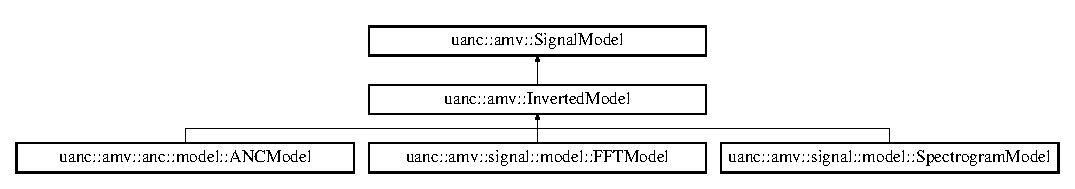
\includegraphics[height=2.089552cm]{classuanc_1_1amv_1_1_signal_model}
\end{center}
\end{figure}
\subsection*{Public Attributes}
\begin{DoxyCompactItemize}
\item 
std\+::shared\+\_\+ptr$<$ Aquila\+::\+Signal\+Source $>$ \hyperlink{classuanc_1_1amv_1_1_signal_model_a608802e04d8ce5d49c730d568f0c3fd7}{left\+\_\+channel}
\begin{DoxyCompactList}\small\item\em Field holds the original samples. \end{DoxyCompactList}\item 
std\+::shared\+\_\+ptr$<$ Aquila\+::\+Signal\+Source $>$ \hyperlink{classuanc_1_1amv_1_1_signal_model_a97081cc1295d40bc9410e883bcc02a84}{right\+\_\+channel}
\begin{DoxyCompactList}\small\item\em Field holds the right samples. \end{DoxyCompactList}\end{DoxyCompactItemize}


\subsection{Detailed Description}
Every model used inside of this application has to be a signal model. 

This class represents the most general model. It basically contains a field with the original signal. This gets used throughout the whole project. 

\subsection{Member Data Documentation}
\index{uanc\+::amv\+::\+Signal\+Model@{uanc\+::amv\+::\+Signal\+Model}!left\+\_\+channel@{left\+\_\+channel}}
\index{left\+\_\+channel@{left\+\_\+channel}!uanc\+::amv\+::\+Signal\+Model@{uanc\+::amv\+::\+Signal\+Model}}
\subsubsection[{\texorpdfstring{left\+\_\+channel}{left_channel}}]{\setlength{\rightskip}{0pt plus 5cm}std\+::shared\+\_\+ptr$<$Aquila\+::\+Signal\+Source$>$ uanc\+::amv\+::\+Signal\+Model\+::left\+\_\+channel}\hypertarget{classuanc_1_1amv_1_1_signal_model_a608802e04d8ce5d49c730d568f0c3fd7}{}\label{classuanc_1_1amv_1_1_signal_model_a608802e04d8ce5d49c730d568f0c3fd7}


Field holds the original samples. 

Holds the original samples, which were read from the hard drive. \index{uanc\+::amv\+::\+Signal\+Model@{uanc\+::amv\+::\+Signal\+Model}!right\+\_\+channel@{right\+\_\+channel}}
\index{right\+\_\+channel@{right\+\_\+channel}!uanc\+::amv\+::\+Signal\+Model@{uanc\+::amv\+::\+Signal\+Model}}
\subsubsection[{\texorpdfstring{right\+\_\+channel}{right_channel}}]{\setlength{\rightskip}{0pt plus 5cm}std\+::shared\+\_\+ptr$<$Aquila\+::\+Signal\+Source$>$ uanc\+::amv\+::\+Signal\+Model\+::right\+\_\+channel}\hypertarget{classuanc_1_1amv_1_1_signal_model_a97081cc1295d40bc9410e883bcc02a84}{}\label{classuanc_1_1amv_1_1_signal_model_a97081cc1295d40bc9410e883bcc02a84}


Field holds the right samples. 

Holds the original samples, which were read from the hard drive. 

The documentation for this class was generated from the following file\+:\begin{DoxyCompactItemize}
\item 
/home/kurt/\+Documents/\+Studium/\+Bachelor\+\_\+\+Praktikum/\+U\+A\+N\+C/\+Code/\+U\+A\+N\+C/amv/\hyperlink{_signal_model_8h}{Signal\+Model.\+h}\end{DoxyCompactItemize}

\hypertarget{classuanc_1_1gui_1_1_signal_plot}{}\section{uanc\+:\+:gui\+:\+:Signal\+Plot Class Reference}
\label{classuanc_1_1gui_1_1_signal_plot}\index{uanc\+::gui\+::\+Signal\+Plot@{uanc\+::gui\+::\+Signal\+Plot}}


{\ttfamily \#include $<$Signal\+Plot.\+h$>$}

Inheritance diagram for uanc\+:\+:gui\+:\+:Signal\+Plot\+:\begin{figure}[H]
\begin{center}
\leavevmode
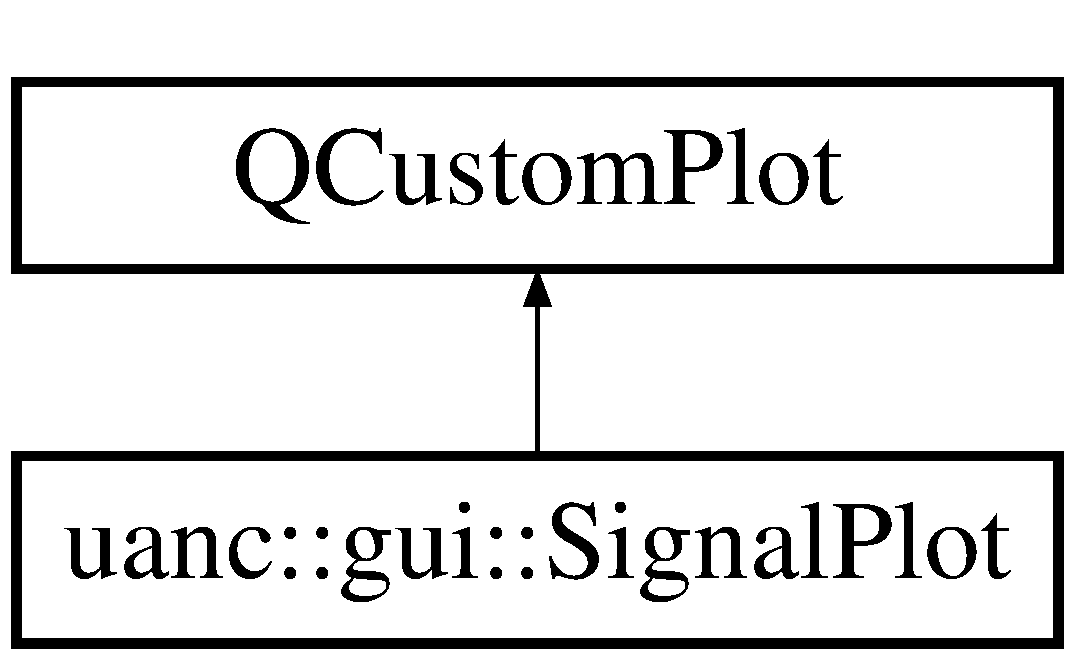
\includegraphics[height=2.000000cm]{classuanc_1_1gui_1_1_signal_plot}
\end{center}
\end{figure}
\subsection*{Public Slots}
\begin{DoxyCompactItemize}
\item 
void \hyperlink{classuanc_1_1gui_1_1_signal_plot_a0475564db8751278d12f1fbbf97328db}{hide\+Error} (bool hide)
\begin{DoxyCompactList}\small\item\em simple set error to visible or not \end{DoxyCompactList}\item 
void \hyperlink{classuanc_1_1gui_1_1_signal_plot_a61480d53076b2778594d19fe2ca984bf}{set\+Centered\+Y\+Axis} (bool b)
\begin{DoxyCompactList}\small\item\em simple set the Y\+Axis to centered or not \end{DoxyCompactList}\end{DoxyCompactItemize}
\subsection*{Public Member Functions}
\begin{DoxyCompactItemize}
\item 
\hyperlink{classuanc_1_1gui_1_1_signal_plot_ad36555db204bd2c73a405312db0741c7}{Signal\+Plot} (\hyperlink{classuanc_1_1gui_1_1_plot_widget}{Plot\+Widget} $\ast$parent)
\begin{DoxyCompactList}\small\item\em The default Constructor. \end{DoxyCompactList}\item 
void \hyperlink{classuanc_1_1gui_1_1_signal_plot_a3177c878d66b3d6fc040114d9e33ec04}{set\+Data} (Q\+C\+P\+Graph\+Data\+Container $\ast$data)
\begin{DoxyCompactList}\small\item\em sets the data to plot the signal \end{DoxyCompactList}\item 
void \hyperlink{classuanc_1_1gui_1_1_signal_plot_a9192356834624ef1369e45aad33ce81b}{set\+Error} (Q\+C\+P\+Graph\+Data\+Container $\ast$error)
\begin{DoxyCompactList}\small\item\em sets the data to plot the signal \end{DoxyCompactList}\item 
void \hyperlink{classuanc_1_1gui_1_1_signal_plot_a64cf6dd1e96f528910d54e129aaddd84}{set\+Range} (double lower, double upper)
\begin{DoxyCompactList}\small\item\em sets the range of the plot \end{DoxyCompactList}\end{DoxyCompactItemize}


\subsection{Constructor \& Destructor Documentation}
\index{uanc\+::gui\+::\+Signal\+Plot@{uanc\+::gui\+::\+Signal\+Plot}!Signal\+Plot@{Signal\+Plot}}
\index{Signal\+Plot@{Signal\+Plot}!uanc\+::gui\+::\+Signal\+Plot@{uanc\+::gui\+::\+Signal\+Plot}}
\subsubsection[{\texorpdfstring{Signal\+Plot(\+Plot\+Widget $\ast$parent)}{SignalPlot(PlotWidget *parent)}}]{\setlength{\rightskip}{0pt plus 5cm}uanc\+::gui\+::\+Signal\+Plot\+::\+Signal\+Plot (
\begin{DoxyParamCaption}
\item[{{\bf Plot\+Widget} $\ast$}]{parent}
\end{DoxyParamCaption}
)}\hypertarget{classuanc_1_1gui_1_1_signal_plot_ad36555db204bd2c73a405312db0741c7}{}\label{classuanc_1_1gui_1_1_signal_plot_ad36555db204bd2c73a405312db0741c7}


The default Constructor. 



\subsection{Member Function Documentation}
\index{uanc\+::gui\+::\+Signal\+Plot@{uanc\+::gui\+::\+Signal\+Plot}!hide\+Error@{hide\+Error}}
\index{hide\+Error@{hide\+Error}!uanc\+::gui\+::\+Signal\+Plot@{uanc\+::gui\+::\+Signal\+Plot}}
\subsubsection[{\texorpdfstring{hide\+Error}{hideError}}]{\setlength{\rightskip}{0pt plus 5cm}void uanc\+::gui\+::\+Signal\+Plot\+::hide\+Error (
\begin{DoxyParamCaption}
\item[{bool}]{hide}
\end{DoxyParamCaption}
)\hspace{0.3cm}{\ttfamily [slot]}}\hypertarget{classuanc_1_1gui_1_1_signal_plot_a0475564db8751278d12f1fbbf97328db}{}\label{classuanc_1_1gui_1_1_signal_plot_a0475564db8751278d12f1fbbf97328db}


simple set error to visible or not 


\begin{DoxyParams}{Parameters}
{\em hide} & boolean to determine wether the error is shown or not \\
\hline
\end{DoxyParams}
\index{uanc\+::gui\+::\+Signal\+Plot@{uanc\+::gui\+::\+Signal\+Plot}!set\+Centered\+Y\+Axis@{set\+Centered\+Y\+Axis}}
\index{set\+Centered\+Y\+Axis@{set\+Centered\+Y\+Axis}!uanc\+::gui\+::\+Signal\+Plot@{uanc\+::gui\+::\+Signal\+Plot}}
\subsubsection[{\texorpdfstring{set\+Centered\+Y\+Axis}{setCenteredYAxis}}]{\setlength{\rightskip}{0pt plus 5cm}void uanc\+::gui\+::\+Signal\+Plot\+::set\+Centered\+Y\+Axis (
\begin{DoxyParamCaption}
\item[{bool}]{b}
\end{DoxyParamCaption}
)\hspace{0.3cm}{\ttfamily [inline]}, {\ttfamily [slot]}}\hypertarget{classuanc_1_1gui_1_1_signal_plot_a61480d53076b2778594d19fe2ca984bf}{}\label{classuanc_1_1gui_1_1_signal_plot_a61480d53076b2778594d19fe2ca984bf}


simple set the Y\+Axis to centered or not 


\begin{DoxyParams}{Parameters}
{\em hide} & boolean to determine wether the Y\+Axis is centered or not \\
\hline
\end{DoxyParams}
\index{uanc\+::gui\+::\+Signal\+Plot@{uanc\+::gui\+::\+Signal\+Plot}!set\+Data@{set\+Data}}
\index{set\+Data@{set\+Data}!uanc\+::gui\+::\+Signal\+Plot@{uanc\+::gui\+::\+Signal\+Plot}}
\subsubsection[{\texorpdfstring{set\+Data(\+Q\+C\+P\+Graph\+Data\+Container $\ast$data)}{setData(QCPGraphDataContainer *data)}}]{\setlength{\rightskip}{0pt plus 5cm}void uanc\+::gui\+::\+Signal\+Plot\+::set\+Data (
\begin{DoxyParamCaption}
\item[{Q\+C\+P\+Graph\+Data\+Container $\ast$}]{data}
\end{DoxyParamCaption}
)}\hypertarget{classuanc_1_1gui_1_1_signal_plot_a3177c878d66b3d6fc040114d9e33ec04}{}\label{classuanc_1_1gui_1_1_signal_plot_a3177c878d66b3d6fc040114d9e33ec04}


sets the data to plot the signal 


\begin{DoxyParams}{Parameters}
{\em data} & this is the data that has to be ploted \\
\hline
\end{DoxyParams}
\index{uanc\+::gui\+::\+Signal\+Plot@{uanc\+::gui\+::\+Signal\+Plot}!set\+Error@{set\+Error}}
\index{set\+Error@{set\+Error}!uanc\+::gui\+::\+Signal\+Plot@{uanc\+::gui\+::\+Signal\+Plot}}
\subsubsection[{\texorpdfstring{set\+Error(\+Q\+C\+P\+Graph\+Data\+Container $\ast$error)}{setError(QCPGraphDataContainer *error)}}]{\setlength{\rightskip}{0pt plus 5cm}void uanc\+::gui\+::\+Signal\+Plot\+::set\+Error (
\begin{DoxyParamCaption}
\item[{Q\+C\+P\+Graph\+Data\+Container $\ast$}]{error}
\end{DoxyParamCaption}
)}\hypertarget{classuanc_1_1gui_1_1_signal_plot_a9192356834624ef1369e45aad33ce81b}{}\label{classuanc_1_1gui_1_1_signal_plot_a9192356834624ef1369e45aad33ce81b}


sets the data to plot the signal 


\begin{DoxyParams}{Parameters}
{\em error} & this is the eroor that has to be ploted \\
\hline
\end{DoxyParams}
\index{uanc\+::gui\+::\+Signal\+Plot@{uanc\+::gui\+::\+Signal\+Plot}!set\+Range@{set\+Range}}
\index{set\+Range@{set\+Range}!uanc\+::gui\+::\+Signal\+Plot@{uanc\+::gui\+::\+Signal\+Plot}}
\subsubsection[{\texorpdfstring{set\+Range(double lower, double upper)}{setRange(double lower, double upper)}}]{\setlength{\rightskip}{0pt plus 5cm}void uanc\+::gui\+::\+Signal\+Plot\+::set\+Range (
\begin{DoxyParamCaption}
\item[{double}]{lower, }
\item[{double}]{upper}
\end{DoxyParamCaption}
)}\hypertarget{classuanc_1_1gui_1_1_signal_plot_a64cf6dd1e96f528910d54e129aaddd84}{}\label{classuanc_1_1gui_1_1_signal_plot_a64cf6dd1e96f528910d54e129aaddd84}


sets the range of the plot 


\begin{DoxyParams}{Parameters}
{\em lower} & the lower border \\
\hline
{\em upper} & the upper border \\
\hline
\end{DoxyParams}


The documentation for this class was generated from the following files\+:\begin{DoxyCompactItemize}
\item 
/ext/local/\+University/\+B\+P/\+Git/\+U\+A\+N\+C/\+Code/\+U\+A\+N\+C/gui/\hyperlink{_signal_plot_8h}{Signal\+Plot.\+h}\item 
/ext/local/\+University/\+B\+P/\+Git/\+U\+A\+N\+C/\+Code/\+U\+A\+N\+C/gui/\hyperlink{_signal_plot_8cpp}{Signal\+Plot.\+cpp}\end{DoxyCompactItemize}

\hypertarget{classuanc_1_1amv_1_1signal_1_1algorithm_1_1_signal_transformation_algorithm}{}\section{uanc\+:\+:amv\+:\+:signal\+:\+:algorithm\+:\+:Signal\+Transformation\+Algorithm$<$ datamodel, viewmodel $>$ Class Template Reference}
\label{classuanc_1_1amv_1_1signal_1_1algorithm_1_1_signal_transformation_algorithm}\index{uanc\+::amv\+::signal\+::algorithm\+::\+Signal\+Transformation\+Algorithm$<$ datamodel, viewmodel $>$@{uanc\+::amv\+::signal\+::algorithm\+::\+Signal\+Transformation\+Algorithm$<$ datamodel, viewmodel $>$}}


Every algorithm used inside has to be derived by this class.  




{\ttfamily \#include $<$Signal\+Transformation\+Algorithm.\+h$>$}

Inheritance diagram for uanc\+:\+:amv\+:\+:signal\+:\+:algorithm\+:\+:Signal\+Transformation\+Algorithm$<$ datamodel, viewmodel $>$\+:\begin{figure}[H]
\begin{center}
\leavevmode
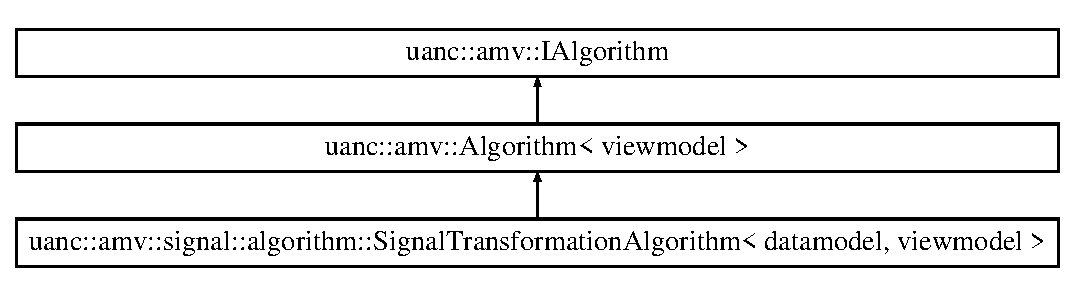
\includegraphics[height=3.000000cm]{classuanc_1_1amv_1_1signal_1_1algorithm_1_1_signal_transformation_algorithm}
\end{center}
\end{figure}
\subsection*{Protected Member Functions}
\begin{DoxyCompactItemize}
\item 
std\+::shared\+\_\+ptr$<$ datamodel $>$ \hyperlink{classuanc_1_1amv_1_1signal_1_1algorithm_1_1_signal_transformation_algorithm_a7118b46dcfdadf8648cf927c4bdd70d0}{execute} (std\+::shared\+\_\+ptr$<$ \hyperlink{classuanc_1_1amv_1_1_inverted_model}{uanc\+::amv\+::\+Inverted\+Model} $>$ input) final
\begin{DoxyCompactList}\small\item\em Executed an algorithm with the given input model. \end{DoxyCompactList}\item 
std\+::shared\+\_\+ptr$<$ datamodel $>$ \hyperlink{classuanc_1_1amv_1_1signal_1_1algorithm_1_1_signal_transformation_algorithm_acb59a47bcaf75198a7f5e3a2f1392942}{get\+Model} ()
\begin{DoxyCompactList}\small\item\em Gets a pointer, to access the model of the algorithm. \end{DoxyCompactList}\item 
virtual void \hyperlink{classuanc_1_1amv_1_1signal_1_1algorithm_1_1_signal_transformation_algorithm_a40dee2d59e84244373cacc9c472514d6}{transform} (std\+::shared\+\_\+ptr$<$ \hyperlink{classuanc_1_1amv_1_1_inverted_model}{uanc\+::amv\+::\+Inverted\+Model} $>$ input)=0
\begin{DoxyCompactList}\small\item\em Inverts the input signal. \end{DoxyCompactList}\end{DoxyCompactItemize}
\subsection*{Additional Inherited Members}


\subsection{Detailed Description}
\subsubsection*{template$<$typename datamodel, typename viewmodel = datamodel$>$\\*
class uanc\+::amv\+::signal\+::algorithm\+::\+Signal\+Transformation\+Algorithm$<$ datamodel, viewmodel $>$}

Every algorithm used inside has to be derived by this class. 

This represents an A\+N\+C\+Algorithm. So every inverting algorithm has to be derived by this. In addition one can specify the data model and the view model. If you want to use only a subset of the data you can specify a view model which is actually a parent of the data model. If there is no view model supplied, they will be handled, as if they are the same


\begin{DoxyTemplParams}{Template Parameters}
{\em datamodel} & The data model to use, has to be inherited from viewmodel \\
\hline
{\em viewmodel} & The view model to use, has to be inherited from \hyperlink{classuanc_1_1amv_1_1_signal_model}{Signal\+Model} \\
\hline
\end{DoxyTemplParams}


\subsection{Member Function Documentation}
\index{uanc\+::amv\+::signal\+::algorithm\+::\+Signal\+Transformation\+Algorithm@{uanc\+::amv\+::signal\+::algorithm\+::\+Signal\+Transformation\+Algorithm}!execute@{execute}}
\index{execute@{execute}!uanc\+::amv\+::signal\+::algorithm\+::\+Signal\+Transformation\+Algorithm@{uanc\+::amv\+::signal\+::algorithm\+::\+Signal\+Transformation\+Algorithm}}
\subsubsection[{\texorpdfstring{execute(std\+::shared\+\_\+ptr$<$ uanc\+::amv\+::\+Inverted\+Model $>$ input) final}{execute(std::shared_ptr< uanc::amv::InvertedModel > input) final}}]{\setlength{\rightskip}{0pt plus 5cm}template$<$typename datamodel, typename viewmodel = datamodel$>$ std\+::shared\+\_\+ptr$<$datamodel$>$ {\bf uanc\+::amv\+::signal\+::algorithm\+::\+Signal\+Transformation\+Algorithm}$<$ datamodel, viewmodel $>$\+::execute (
\begin{DoxyParamCaption}
\item[{std\+::shared\+\_\+ptr$<$ {\bf uanc\+::amv\+::\+Inverted\+Model} $>$}]{input}
\end{DoxyParamCaption}
)\hspace{0.3cm}{\ttfamily [inline]}, {\ttfamily [final]}, {\ttfamily [protected]}, {\ttfamily [virtual]}}\hypertarget{classuanc_1_1amv_1_1signal_1_1algorithm_1_1_signal_transformation_algorithm_a7118b46dcfdadf8648cf927c4bdd70d0}{}\label{classuanc_1_1amv_1_1signal_1_1algorithm_1_1_signal_transformation_algorithm_a7118b46dcfdadf8648cf927c4bdd70d0}


Executed an algorithm with the given input model. 

This method first all gets an empty model from the deriving class. Afterwards it inverts the signal and passed back the model, which was created during the execution stage.


\begin{DoxyParams}[1]{Parameters}
\mbox{\tt in}  & {\em input} & The input model of the signal.\\
\hline
\end{DoxyParams}
\begin{DoxyReturn}{Returns}
The created model from the data of the inversion. 
\end{DoxyReturn}


Implements \hyperlink{classuanc_1_1amv_1_1_algorithm_a3a0bd5e6e8cc1a3f9bd9d9b384e121b5}{uanc\+::amv\+::\+Algorithm$<$ viewmodel $>$}.

\index{uanc\+::amv\+::signal\+::algorithm\+::\+Signal\+Transformation\+Algorithm@{uanc\+::amv\+::signal\+::algorithm\+::\+Signal\+Transformation\+Algorithm}!get\+Model@{get\+Model}}
\index{get\+Model@{get\+Model}!uanc\+::amv\+::signal\+::algorithm\+::\+Signal\+Transformation\+Algorithm@{uanc\+::amv\+::signal\+::algorithm\+::\+Signal\+Transformation\+Algorithm}}
\subsubsection[{\texorpdfstring{get\+Model()}{getModel()}}]{\setlength{\rightskip}{0pt plus 5cm}template$<$typename datamodel, typename viewmodel = datamodel$>$ std\+::shared\+\_\+ptr$<$datamodel$>$ {\bf uanc\+::amv\+::signal\+::algorithm\+::\+Signal\+Transformation\+Algorithm}$<$ datamodel, viewmodel $>$\+::get\+Model (
\begin{DoxyParamCaption}
{}
\end{DoxyParamCaption}
)\hspace{0.3cm}{\ttfamily [inline]}, {\ttfamily [protected]}}\hypertarget{classuanc_1_1amv_1_1signal_1_1algorithm_1_1_signal_transformation_algorithm_acb59a47bcaf75198a7f5e3a2f1392942}{}\label{classuanc_1_1amv_1_1signal_1_1algorithm_1_1_signal_transformation_algorithm_acb59a47bcaf75198a7f5e3a2f1392942}


Gets a pointer, to access the model of the algorithm. 

Getter for the model used inside of the algorithm. This pointer can be modified by deriving classes to manipulate the model.

\begin{DoxyReturn}{Returns}
The pointer to the data model stored inside. 
\end{DoxyReturn}
\index{uanc\+::amv\+::signal\+::algorithm\+::\+Signal\+Transformation\+Algorithm@{uanc\+::amv\+::signal\+::algorithm\+::\+Signal\+Transformation\+Algorithm}!transform@{transform}}
\index{transform@{transform}!uanc\+::amv\+::signal\+::algorithm\+::\+Signal\+Transformation\+Algorithm@{uanc\+::amv\+::signal\+::algorithm\+::\+Signal\+Transformation\+Algorithm}}
\subsubsection[{\texorpdfstring{transform(std\+::shared\+\_\+ptr$<$ uanc\+::amv\+::\+Inverted\+Model $>$ input)=0}{transform(std::shared_ptr< uanc::amv::InvertedModel > input)=0}}]{\setlength{\rightskip}{0pt plus 5cm}template$<$typename datamodel, typename viewmodel = datamodel$>$ virtual void {\bf uanc\+::amv\+::signal\+::algorithm\+::\+Signal\+Transformation\+Algorithm}$<$ datamodel, viewmodel $>$\+::transform (
\begin{DoxyParamCaption}
\item[{std\+::shared\+\_\+ptr$<$ {\bf uanc\+::amv\+::\+Inverted\+Model} $>$}]{input}
\end{DoxyParamCaption}
)\hspace{0.3cm}{\ttfamily [protected]}, {\ttfamily [pure virtual]}}\hypertarget{classuanc_1_1amv_1_1signal_1_1algorithm_1_1_signal_transformation_algorithm_a40dee2d59e84244373cacc9c472514d6}{}\label{classuanc_1_1amv_1_1signal_1_1algorithm_1_1_signal_transformation_algorithm_a40dee2d59e84244373cacc9c472514d6}


Inverts the input signal. 

This is actually capable of transforming the input model into another data representation, which is then used to display it inside of the gui.


\begin{DoxyParams}{Parameters}
{\em input} & The input model containing the original signal. \\
\hline
\end{DoxyParams}


Implemented in \hyperlink{classuanc_1_1amv_1_1signal_1_1algorithm_1_1_f_f_t_transformation_algorithm_a0748e30e870a462a10220cb07c784f2a}{uanc\+::amv\+::signal\+::algorithm\+::\+F\+F\+T\+Transformation\+Algorithm}, \hyperlink{classuanc_1_1amv_1_1signal_1_1algorithm_1_1_identity_transformation_algorithm_aac5f7f10ab44d7f8625eb5dbb72e5c44}{uanc\+::amv\+::signal\+::algorithm\+::\+Identity\+Transformation\+Algorithm}, and \hyperlink{classuanc_1_1amv_1_1signal_1_1algorithm_1_1_spectrogram_transformation_algorithm_a988bc9d4cc15eafb384ed5c81885ef43}{uanc\+::amv\+::signal\+::algorithm\+::\+Spectrogram\+Transformation\+Algorithm}.



The documentation for this class was generated from the following file\+:\begin{DoxyCompactItemize}
\item 
/ext/local/\+University/\+B\+P/\+Git/\+U\+A\+N\+C/\+Code/\+U\+A\+N\+C/amv/signal/algorithm/\hyperlink{_signal_transformation_algorithm_8h}{Signal\+Transformation\+Algorithm.\+h}\end{DoxyCompactItemize}

\hypertarget{classuanc_1_1amv_1_1signal_1_1view_1_1_signal_view}{}\section{uanc\+:\+:amv\+:\+:signal\+:\+:view\+:\+:Signal\+View Class Reference}
\label{classuanc_1_1amv_1_1signal_1_1view_1_1_signal_view}\index{uanc\+::amv\+::signal\+::view\+::\+Signal\+View@{uanc\+::amv\+::signal\+::view\+::\+Signal\+View}}


Represents a \hyperlink{classuanc_1_1amv_1_1signal_1_1view_1_1_signal_view}{Signal\+View}.  




{\ttfamily \#include $<$Signal\+View.\+h$>$}

Inheritance diagram for uanc\+:\+:amv\+:\+:signal\+:\+:view\+:\+:Signal\+View\+:\begin{figure}[H]
\begin{center}
\leavevmode
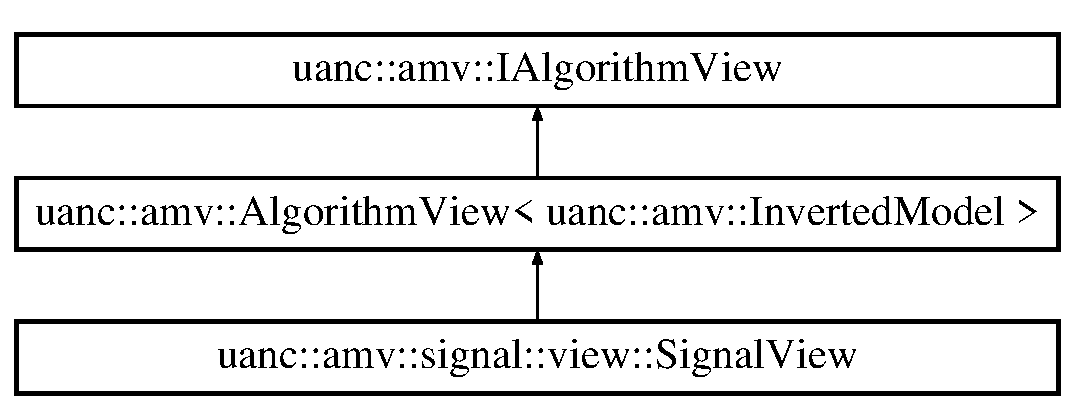
\includegraphics[height=3.000000cm]{classuanc_1_1amv_1_1signal_1_1view_1_1_signal_view}
\end{center}
\end{figure}
\subsection*{Public Member Functions}
\begin{DoxyCompactItemize}
\item 
Q\+Widget $\ast$ \hyperlink{classuanc_1_1amv_1_1signal_1_1view_1_1_signal_view_a8b42dd84baf3c0730640ddb87db69735}{produce\+Widget} () final
\begin{DoxyCompactList}\small\item\em Gets the complete widget. \end{DoxyCompactList}\item 
void \hyperlink{classuanc_1_1amv_1_1signal_1_1view_1_1_signal_view_a9c7eb492154e043e671549d2c71d94bc}{set\+Data} (std\+::shared\+\_\+ptr$<$ \hyperlink{classuanc_1_1amv_1_1_inverted_model}{uanc\+::amv\+::\+Inverted\+Model} $>$ data) final
\begin{DoxyCompactList}\small\item\em This method applies the model data. \end{DoxyCompactList}\end{DoxyCompactItemize}


\subsection{Detailed Description}
Represents a \hyperlink{classuanc_1_1amv_1_1signal_1_1view_1_1_signal_view}{Signal\+View}. 

This represents a general \hyperlink{classuanc_1_1amv_1_1signal_1_1view_1_1_signal_view}{Signal\+View}. It operates on an \hyperlink{classuanc_1_1amv_1_1_signal_model}{Signal\+Model}. It basically shows a plot of the original signal. 

\subsection{Member Function Documentation}
\index{uanc\+::amv\+::signal\+::view\+::\+Signal\+View@{uanc\+::amv\+::signal\+::view\+::\+Signal\+View}!produce\+Widget@{produce\+Widget}}
\index{produce\+Widget@{produce\+Widget}!uanc\+::amv\+::signal\+::view\+::\+Signal\+View@{uanc\+::amv\+::signal\+::view\+::\+Signal\+View}}
\subsubsection[{\texorpdfstring{produce\+Widget() final}{produceWidget() final}}]{\setlength{\rightskip}{0pt plus 5cm}Q\+Widget $\ast$ uanc\+::amv\+::signal\+::view\+::\+Signal\+View\+::produce\+Widget (
\begin{DoxyParamCaption}
{}
\end{DoxyParamCaption}
)\hspace{0.3cm}{\ttfamily [final]}, {\ttfamily [virtual]}}\hypertarget{classuanc_1_1amv_1_1signal_1_1view_1_1_signal_view_a8b42dd84baf3c0730640ddb87db69735}{}\label{classuanc_1_1amv_1_1signal_1_1view_1_1_signal_view_a8b42dd84baf3c0730640ddb87db69735}


Gets the complete widget. 

This function is used to retrieve the widget from the view. It gets used for integration the main application. It creates a Plotwidget inside of a Q\+Widget and passes this back.

\begin{DoxyReturn}{Returns}
The created widget.
\end{DoxyReturn}
This function is used to retrieve the widget from the view. It gets used for integration the main application. It creates a Plotwidget inside of a Q\+Widget and passes this back. Uses the singleton pattern to ensure the unique creation of the widget.

\begin{DoxyReturn}{Returns}
The created widget. 
\end{DoxyReturn}


Implements \hyperlink{classuanc_1_1amv_1_1_i_algorithm_view_ab9d06a0b43db57244868f10dae8e09e5}{uanc\+::amv\+::\+I\+Algorithm\+View}.

\index{uanc\+::amv\+::signal\+::view\+::\+Signal\+View@{uanc\+::amv\+::signal\+::view\+::\+Signal\+View}!set\+Data@{set\+Data}}
\index{set\+Data@{set\+Data}!uanc\+::amv\+::signal\+::view\+::\+Signal\+View@{uanc\+::amv\+::signal\+::view\+::\+Signal\+View}}
\subsubsection[{\texorpdfstring{set\+Data(std\+::shared\+\_\+ptr$<$ uanc\+::amv\+::\+Inverted\+Model $>$ data) final}{setData(std::shared_ptr< uanc::amv::InvertedModel > data) final}}]{\setlength{\rightskip}{0pt plus 5cm}void uanc\+::amv\+::signal\+::view\+::\+Signal\+View\+::set\+Data (
\begin{DoxyParamCaption}
\item[{std\+::shared\+\_\+ptr$<$ {\bf uanc\+::amv\+::\+Inverted\+Model} $>$}]{data}
\end{DoxyParamCaption}
)\hspace{0.3cm}{\ttfamily [final]}, {\ttfamily [virtual]}}\hypertarget{classuanc_1_1amv_1_1signal_1_1view_1_1_signal_view_a9c7eb492154e043e671549d2c71d94bc}{}\label{classuanc_1_1amv_1_1signal_1_1view_1_1_signal_view_a9c7eb492154e043e671549d2c71d94bc}


This method applies the model data. 

This method simply takes the passed data and places it inside of the view at the appropriate places.


\begin{DoxyParams}{Parameters}
{\em data} & The applied data. \\
\hline
\end{DoxyParams}


Implements \hyperlink{classuanc_1_1amv_1_1_algorithm_view_ad656cf5223a66a942441ee39f44f65a3}{uanc\+::amv\+::\+Algorithm\+View$<$ uanc\+::amv\+::\+Inverted\+Model $>$}.



The documentation for this class was generated from the following files\+:\begin{DoxyCompactItemize}
\item 
/ext/local/\+University/\+B\+P/\+Git/\+U\+A\+N\+C/\+Code/\+U\+A\+N\+C/amv/signal/view/\hyperlink{_signal_view_8h}{Signal\+View.\+h}\item 
/ext/local/\+University/\+B\+P/\+Git/\+U\+A\+N\+C/\+Code/\+U\+A\+N\+C/amv/signal/view/\hyperlink{_signal_view_8cpp}{Signal\+View.\+cpp}\end{DoxyCompactItemize}

\hypertarget{classuanc_1_1gui_1_1_signal_view_widget}{}\section{uanc\+:\+:gui\+:\+:Signal\+View\+Widget Class Reference}
\label{classuanc_1_1gui_1_1_signal_view_widget}\index{uanc\+::gui\+::\+Signal\+View\+Widget@{uanc\+::gui\+::\+Signal\+View\+Widget}}


{\ttfamily \#include $<$Signal\+View\+Widget.\+h$>$}

Inheritance diagram for uanc\+:\+:gui\+:\+:Signal\+View\+Widget\+:\begin{figure}[H]
\begin{center}
\leavevmode
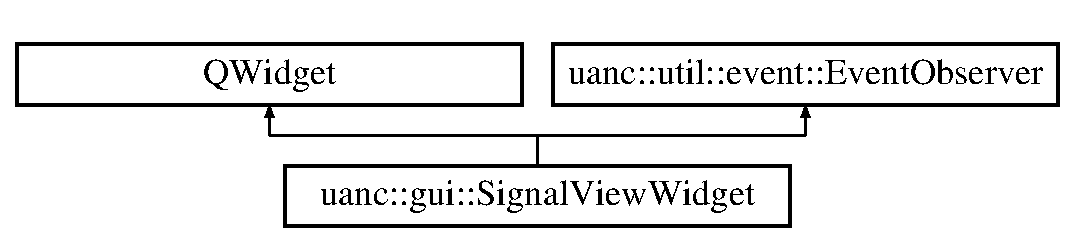
\includegraphics[height=2.000000cm]{classuanc_1_1gui_1_1_signal_view_widget}
\end{center}
\end{figure}
\subsection*{Public Member Functions}
\begin{DoxyCompactItemize}
\item 
\hyperlink{classuanc_1_1gui_1_1_signal_view_widget_aeffeeef7831e71d328e9ec0ae02a778c}{Signal\+View\+Widget} (bool has\+Error=true)
\item 
void \hyperlink{classuanc_1_1gui_1_1_signal_view_widget_a6f69d9363e91c997725a510284fc2f94}{set\+Signal\+Model} (std\+::shared\+\_\+ptr$<$ \hyperlink{classuanc_1_1amv_1_1_inverted_model}{Inverted\+Model} $>$ signal\+Model)
\item 
void \hyperlink{classuanc_1_1gui_1_1_signal_view_widget_a2f070824372de0e83960814229d93b46}{triggered} (\hyperlink{namespaceuanc_1_1util_1_1event_a63f690675589114db9c6bcbe6f1088a4}{Events} event, \hyperlink{classuanc_1_1util_1_1event_1_1_event_container}{Event\+Container} data) final
\begin{DoxyCompactList}\small\item\em Override to catch event. \end{DoxyCompactList}\end{DoxyCompactItemize}
\subsection*{Additional Inherited Members}


\subsection{Constructor \& Destructor Documentation}
\index{uanc\+::gui\+::\+Signal\+View\+Widget@{uanc\+::gui\+::\+Signal\+View\+Widget}!Signal\+View\+Widget@{Signal\+View\+Widget}}
\index{Signal\+View\+Widget@{Signal\+View\+Widget}!uanc\+::gui\+::\+Signal\+View\+Widget@{uanc\+::gui\+::\+Signal\+View\+Widget}}
\subsubsection[{\texorpdfstring{Signal\+View\+Widget(bool has\+Error=true)}{SignalViewWidget(bool hasError=true)}}]{\setlength{\rightskip}{0pt plus 5cm}uanc\+::gui\+::\+Signal\+View\+Widget\+::\+Signal\+View\+Widget (
\begin{DoxyParamCaption}
\item[{bool}]{has\+Error = {\ttfamily true}}
\end{DoxyParamCaption}
)\hspace{0.3cm}{\ttfamily [inline]}}\hypertarget{classuanc_1_1gui_1_1_signal_view_widget_aeffeeef7831e71d328e9ec0ae02a778c}{}\label{classuanc_1_1gui_1_1_signal_view_widget_aeffeeef7831e71d328e9ec0ae02a778c}
Default constructore for the signal view widget.


\begin{DoxyParams}{Parameters}
{\em id} & The unique id of this widget. \\
\hline
{\em has\+Error} & True, if it has error. \\
\hline
\end{DoxyParams}


\subsection{Member Function Documentation}
\index{uanc\+::gui\+::\+Signal\+View\+Widget@{uanc\+::gui\+::\+Signal\+View\+Widget}!set\+Signal\+Model@{set\+Signal\+Model}}
\index{set\+Signal\+Model@{set\+Signal\+Model}!uanc\+::gui\+::\+Signal\+View\+Widget@{uanc\+::gui\+::\+Signal\+View\+Widget}}
\subsubsection[{\texorpdfstring{set\+Signal\+Model(std\+::shared\+\_\+ptr$<$ Inverted\+Model $>$ signal\+Model)}{setSignalModel(std::shared_ptr< InvertedModel > signalModel)}}]{\setlength{\rightskip}{0pt plus 5cm}void uanc\+::gui\+::\+Signal\+View\+Widget\+::set\+Signal\+Model (
\begin{DoxyParamCaption}
\item[{std\+::shared\+\_\+ptr$<$ {\bf Inverted\+Model} $>$}]{signal\+Model}
\end{DoxyParamCaption}
)\hspace{0.3cm}{\ttfamily [inline]}}\hypertarget{classuanc_1_1gui_1_1_signal_view_widget_a6f69d9363e91c997725a510284fc2f94}{}\label{classuanc_1_1gui_1_1_signal_view_widget_a6f69d9363e91c997725a510284fc2f94}
This method sets the signal model internally.


\begin{DoxyParams}{Parameters}
{\em signal\+Model} & The signal model to set. \\
\hline
\end{DoxyParams}
\index{uanc\+::gui\+::\+Signal\+View\+Widget@{uanc\+::gui\+::\+Signal\+View\+Widget}!triggered@{triggered}}
\index{triggered@{triggered}!uanc\+::gui\+::\+Signal\+View\+Widget@{uanc\+::gui\+::\+Signal\+View\+Widget}}
\subsubsection[{\texorpdfstring{triggered(\+Events event, Event\+Container data) final}{triggered(Events event, EventContainer data) final}}]{\setlength{\rightskip}{0pt plus 5cm}void uanc\+::gui\+::\+Signal\+View\+Widget\+::triggered (
\begin{DoxyParamCaption}
\item[{{\bf Events}}]{event, }
\item[{{\bf Event\+Container}}]{data}
\end{DoxyParamCaption}
)\hspace{0.3cm}{\ttfamily [inline]}, {\ttfamily [final]}, {\ttfamily [virtual]}}\hypertarget{classuanc_1_1gui_1_1_signal_view_widget_a2f070824372de0e83960814229d93b46}{}\label{classuanc_1_1gui_1_1_signal_view_widget_a2f070824372de0e83960814229d93b46}


Override to catch event. 

This can be used, to integrate a handling to a specific event.


\begin{DoxyParams}{Parameters}
{\em event} & The event which should be triggered. \\
\hline
{\em data} & The data to supply. \\
\hline
\end{DoxyParams}


Implements \hyperlink{classuanc_1_1util_1_1event_1_1_event_observer_af1640e34db3379eaba8c817a92199807}{uanc\+::util\+::event\+::\+Event\+Observer}.



The documentation for this class was generated from the following file\+:\begin{DoxyCompactItemize}
\item 
/home/kurt/\+Documents/\+Studium/\+Bachelor\+\_\+\+Praktikum/\+U\+A\+N\+C/\+Code/\+U\+A\+N\+C/gui/\hyperlink{_signal_view_widget_8h}{Signal\+View\+Widget.\+h}\end{DoxyCompactItemize}

\hypertarget{classuanc_1_1amv_1_1signal_1_1model_1_1_spectrogram_model}{}\section{uanc\+:\+:amv\+:\+:signal\+:\+:model\+:\+:Spectrogram\+Model Class Reference}
\label{classuanc_1_1amv_1_1signal_1_1model_1_1_spectrogram_model}\index{uanc\+::amv\+::signal\+::model\+::\+Spectrogram\+Model@{uanc\+::amv\+::signal\+::model\+::\+Spectrogram\+Model}}


This is a model for the transformation of a signal to a spectrogram representation.  




{\ttfamily \#include $<$Spectrogram\+Model.\+h$>$}

Inheritance diagram for uanc\+:\+:amv\+:\+:signal\+:\+:model\+:\+:Spectrogram\+Model\+:\begin{figure}[H]
\begin{center}
\leavevmode
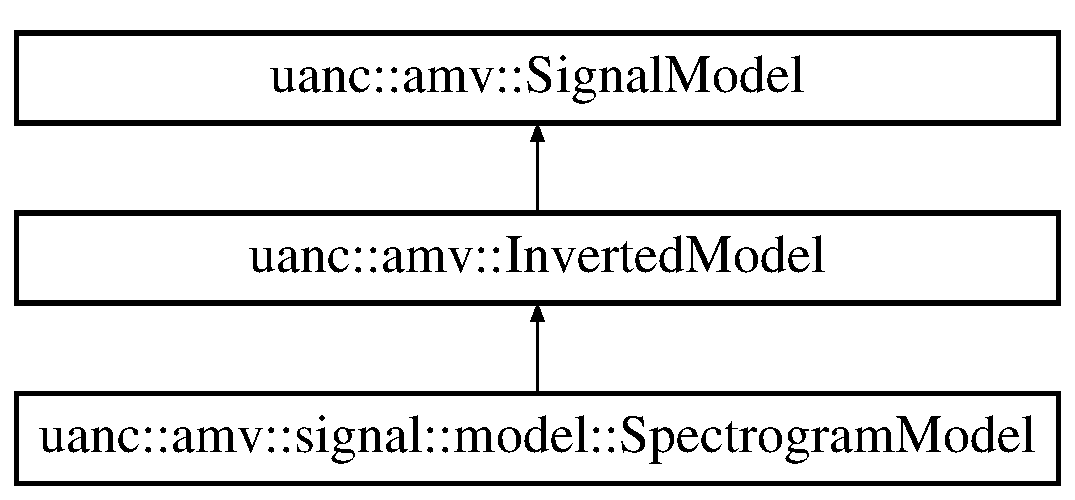
\includegraphics[height=3.000000cm]{classuanc_1_1amv_1_1signal_1_1model_1_1_spectrogram_model}
\end{center}
\end{figure}
\subsection*{Public Attributes}
\begin{DoxyCompactItemize}
\item 
std\+::shared\+\_\+ptr$<$ Aquila\+::\+Spectrogram $>$ \hyperlink{classuanc_1_1amv_1_1signal_1_1model_1_1_spectrogram_model_accb3ed97c155fdec9022bb2d5b106015}{left\+\_\+spectrum}
\begin{DoxyCompactList}\small\item\em Holds the spectrum. \end{DoxyCompactList}\item 
std\+::shared\+\_\+ptr$<$ Aquila\+::\+Spectrogram $>$ \hyperlink{classuanc_1_1amv_1_1signal_1_1model_1_1_spectrogram_model_a3a3559cdc08ae00f3617de962e606c4a}{right\+\_\+spectrum}
\begin{DoxyCompactList}\small\item\em Holds the spectrum. \end{DoxyCompactList}\end{DoxyCompactItemize}


\subsection{Detailed Description}
This is a model for the transformation of a signal to a spectrogram representation. 

It used by the Fourier\+Transformation\+Algorithm. 

\subsection{Member Data Documentation}
\index{uanc\+::amv\+::signal\+::model\+::\+Spectrogram\+Model@{uanc\+::amv\+::signal\+::model\+::\+Spectrogram\+Model}!left\+\_\+spectrum@{left\+\_\+spectrum}}
\index{left\+\_\+spectrum@{left\+\_\+spectrum}!uanc\+::amv\+::signal\+::model\+::\+Spectrogram\+Model@{uanc\+::amv\+::signal\+::model\+::\+Spectrogram\+Model}}
\subsubsection[{\texorpdfstring{left\+\_\+spectrum}{left_spectrum}}]{\setlength{\rightskip}{0pt plus 5cm}std\+::shared\+\_\+ptr$<$Aquila\+::\+Spectrogram$>$ uanc\+::amv\+::signal\+::model\+::\+Spectrogram\+Model\+::left\+\_\+spectrum}\hypertarget{classuanc_1_1amv_1_1signal_1_1model_1_1_spectrogram_model_accb3ed97c155fdec9022bb2d5b106015}{}\label{classuanc_1_1amv_1_1signal_1_1model_1_1_spectrogram_model_accb3ed97c155fdec9022bb2d5b106015}


Holds the spectrum. 

This field holds the spectrum of the original signal. \index{uanc\+::amv\+::signal\+::model\+::\+Spectrogram\+Model@{uanc\+::amv\+::signal\+::model\+::\+Spectrogram\+Model}!right\+\_\+spectrum@{right\+\_\+spectrum}}
\index{right\+\_\+spectrum@{right\+\_\+spectrum}!uanc\+::amv\+::signal\+::model\+::\+Spectrogram\+Model@{uanc\+::amv\+::signal\+::model\+::\+Spectrogram\+Model}}
\subsubsection[{\texorpdfstring{right\+\_\+spectrum}{right_spectrum}}]{\setlength{\rightskip}{0pt plus 5cm}std\+::shared\+\_\+ptr$<$Aquila\+::\+Spectrogram$>$ uanc\+::amv\+::signal\+::model\+::\+Spectrogram\+Model\+::right\+\_\+spectrum}\hypertarget{classuanc_1_1amv_1_1signal_1_1model_1_1_spectrogram_model_a3a3559cdc08ae00f3617de962e606c4a}{}\label{classuanc_1_1amv_1_1signal_1_1model_1_1_spectrogram_model_a3a3559cdc08ae00f3617de962e606c4a}


Holds the spectrum. 

This field holds the spectrum of the original signal. 

The documentation for this class was generated from the following file\+:\begin{DoxyCompactItemize}
\item 
/home/kurt/\+Documents/\+Studium/\+Bachelor\+\_\+\+Praktikum/\+U\+A\+N\+C/\+Code/\+U\+A\+N\+C/amv/signal/model/\hyperlink{_spectrogram_model_8h}{Spectrogram\+Model.\+h}\end{DoxyCompactItemize}

\hypertarget{classuanc_1_1amv_1_1signal_1_1algorithm_1_1_spectrogram_transformation_algorithm}{}\section{uanc\+:\+:amv\+:\+:signal\+:\+:algorithm\+:\+:Spectrogram\+Transformation\+Algorithm Class Reference}
\label{classuanc_1_1amv_1_1signal_1_1algorithm_1_1_spectrogram_transformation_algorithm}\index{uanc\+::amv\+::signal\+::algorithm\+::\+Spectrogram\+Transformation\+Algorithm@{uanc\+::amv\+::signal\+::algorithm\+::\+Spectrogram\+Transformation\+Algorithm}}


Transforms the view of a signal into a spectrogram.  




{\ttfamily \#include $<$Spectrogram\+Transformation\+Algorithm.\+h$>$}

Inheritance diagram for uanc\+:\+:amv\+:\+:signal\+:\+:algorithm\+:\+:Spectrogram\+Transformation\+Algorithm\+:\begin{figure}[H]
\begin{center}
\leavevmode
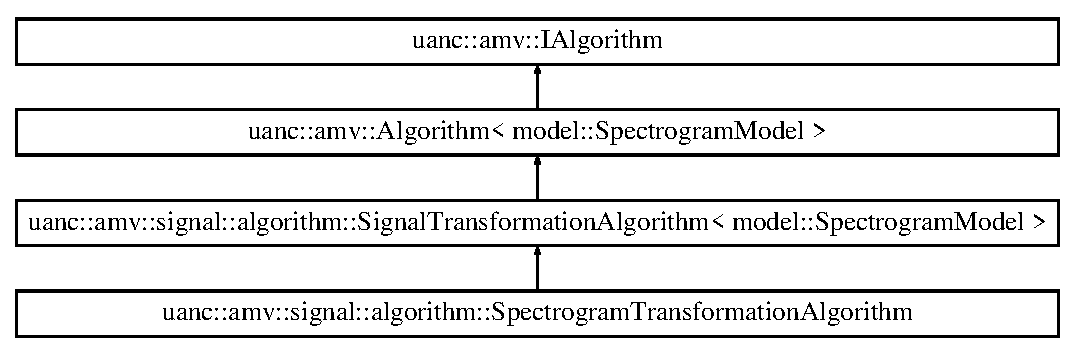
\includegraphics[height=4.000000cm]{classuanc_1_1amv_1_1signal_1_1algorithm_1_1_spectrogram_transformation_algorithm}
\end{center}
\end{figure}
\subsection*{Public Member Functions}
\begin{DoxyCompactItemize}
\item 
std\+::string \hyperlink{classuanc_1_1amv_1_1signal_1_1algorithm_1_1_spectrogram_transformation_algorithm_ab3f352205061c1b6aaa87c6e7c3dbece}{get\+Name} () final
\begin{DoxyCompactList}\small\item\em Returns the name of the transformed data representation. \end{DoxyCompactList}\item 
void \hyperlink{classuanc_1_1amv_1_1signal_1_1algorithm_1_1_spectrogram_transformation_algorithm_a988bc9d4cc15eafb384ed5c81885ef43}{transform} (std\+::shared\+\_\+ptr$<$ \hyperlink{classuanc_1_1amv_1_1_inverted_model}{uanc\+::amv\+::\+Inverted\+Model} $>$ in) final
\begin{DoxyCompactList}\small\item\em Simply saves the input signal to the output. \end{DoxyCompactList}\item 
\hyperlink{classuanc_1_1amv_1_1_algorithm}{Algorithm} $\ast$ \hyperlink{classuanc_1_1amv_1_1signal_1_1algorithm_1_1_spectrogram_transformation_algorithm_a6efc3617627883a6d2acc52e582dd5a3}{clone} () final
\begin{DoxyCompactList}\small\item\em Clones the current instance. \end{DoxyCompactList}\end{DoxyCompactItemize}
\subsection*{Protected Member Functions}
\begin{DoxyCompactItemize}
\item 
\hyperlink{classuanc_1_1amv_1_1_algorithm_view}{Algorithm\+View}$<$ \hyperlink{classuanc_1_1amv_1_1signal_1_1model_1_1_spectrogram_model}{model\+::\+Spectrogram\+Model} $>$ $\ast$ \hyperlink{classuanc_1_1amv_1_1signal_1_1algorithm_1_1_spectrogram_transformation_algorithm_aa36e723764a73225f490cf6baf693a21}{construct\+View} () final
\begin{DoxyCompactList}\small\item\em Constructs a view, which can handle an Fourier\+Model. \end{DoxyCompactList}\end{DoxyCompactItemize}


\subsection{Detailed Description}
Transforms the view of a signal into a spectrogram. 

This transformation basically adds some fourier room information to the basis \hyperlink{classuanc_1_1amv_1_1_signal_model}{Signal\+Model}. 

\subsection{Member Function Documentation}
\index{uanc\+::amv\+::signal\+::algorithm\+::\+Spectrogram\+Transformation\+Algorithm@{uanc\+::amv\+::signal\+::algorithm\+::\+Spectrogram\+Transformation\+Algorithm}!clone@{clone}}
\index{clone@{clone}!uanc\+::amv\+::signal\+::algorithm\+::\+Spectrogram\+Transformation\+Algorithm@{uanc\+::amv\+::signal\+::algorithm\+::\+Spectrogram\+Transformation\+Algorithm}}
\subsubsection[{\texorpdfstring{clone() final}{clone() final}}]{\setlength{\rightskip}{0pt plus 5cm}{\bf Algorithm}$\ast$ uanc\+::amv\+::signal\+::algorithm\+::\+Spectrogram\+Transformation\+Algorithm\+::clone (
\begin{DoxyParamCaption}
{}
\end{DoxyParamCaption}
)\hspace{0.3cm}{\ttfamily [inline]}, {\ttfamily [final]}, {\ttfamily [virtual]}}\hypertarget{classuanc_1_1amv_1_1signal_1_1algorithm_1_1_spectrogram_transformation_algorithm_a6efc3617627883a6d2acc52e582dd5a3}{}\label{classuanc_1_1amv_1_1signal_1_1algorithm_1_1_spectrogram_transformation_algorithm_a6efc3617627883a6d2acc52e582dd5a3}


Clones the current instance. 

This is basically the prototype pattern. It gets used to create an copy of the current Fourier\+Transformation\+Algorithm. To do so it simply creates a new instance.

\begin{DoxyReturn}{Returns}
The cloned algorithm. 
\end{DoxyReturn}


Implements \hyperlink{classuanc_1_1amv_1_1_i_algorithm_af6fcbfa35f460363c2cc7e6134af8dc7}{uanc\+::amv\+::\+I\+Algorithm}.

\index{uanc\+::amv\+::signal\+::algorithm\+::\+Spectrogram\+Transformation\+Algorithm@{uanc\+::amv\+::signal\+::algorithm\+::\+Spectrogram\+Transformation\+Algorithm}!construct\+View@{construct\+View}}
\index{construct\+View@{construct\+View}!uanc\+::amv\+::signal\+::algorithm\+::\+Spectrogram\+Transformation\+Algorithm@{uanc\+::amv\+::signal\+::algorithm\+::\+Spectrogram\+Transformation\+Algorithm}}
\subsubsection[{\texorpdfstring{construct\+View() final}{constructView() final}}]{\setlength{\rightskip}{0pt plus 5cm}{\bf Algorithm\+View}$<${\bf model\+::\+Spectrogram\+Model}$>$$\ast$ uanc\+::amv\+::signal\+::algorithm\+::\+Spectrogram\+Transformation\+Algorithm\+::construct\+View (
\begin{DoxyParamCaption}
{}
\end{DoxyParamCaption}
)\hspace{0.3cm}{\ttfamily [inline]}, {\ttfamily [final]}, {\ttfamily [protected]}, {\ttfamily [virtual]}}\hypertarget{classuanc_1_1amv_1_1signal_1_1algorithm_1_1_spectrogram_transformation_algorithm_aa36e723764a73225f490cf6baf693a21}{}\label{classuanc_1_1amv_1_1signal_1_1algorithm_1_1_spectrogram_transformation_algorithm_aa36e723764a73225f490cf6baf693a21}


Constructs a view, which can handle an Fourier\+Model. 

This view basically display the standard information of the algorithm.

\begin{DoxyReturn}{Returns}
The created algorithm view.. 
\end{DoxyReturn}


Implements \hyperlink{classuanc_1_1amv_1_1_algorithm_af5561072283ed19634893263c95a4b6e}{uanc\+::amv\+::\+Algorithm$<$ model\+::\+Spectrogram\+Model $>$}.

\index{uanc\+::amv\+::signal\+::algorithm\+::\+Spectrogram\+Transformation\+Algorithm@{uanc\+::amv\+::signal\+::algorithm\+::\+Spectrogram\+Transformation\+Algorithm}!get\+Name@{get\+Name}}
\index{get\+Name@{get\+Name}!uanc\+::amv\+::signal\+::algorithm\+::\+Spectrogram\+Transformation\+Algorithm@{uanc\+::amv\+::signal\+::algorithm\+::\+Spectrogram\+Transformation\+Algorithm}}
\subsubsection[{\texorpdfstring{get\+Name() final}{getName() final}}]{\setlength{\rightskip}{0pt plus 5cm}std\+::string uanc\+::amv\+::signal\+::algorithm\+::\+Spectrogram\+Transformation\+Algorithm\+::get\+Name (
\begin{DoxyParamCaption}
{}
\end{DoxyParamCaption}
)\hspace{0.3cm}{\ttfamily [inline]}, {\ttfamily [final]}, {\ttfamily [virtual]}}\hypertarget{classuanc_1_1amv_1_1signal_1_1algorithm_1_1_spectrogram_transformation_algorithm_ab3f352205061c1b6aaa87c6e7c3dbece}{}\label{classuanc_1_1amv_1_1signal_1_1algorithm_1_1_spectrogram_transformation_algorithm_ab3f352205061c1b6aaa87c6e7c3dbece}


Returns the name of the transformed data representation. 

Simply passes back the name of the data transformation

\begin{DoxyReturn}{Returns}
Name of the data transformation 
\end{DoxyReturn}


Implements \hyperlink{classuanc_1_1amv_1_1_i_algorithm_a4935ab2fdacccf7df35d6fb596075edb}{uanc\+::amv\+::\+I\+Algorithm}.

\index{uanc\+::amv\+::signal\+::algorithm\+::\+Spectrogram\+Transformation\+Algorithm@{uanc\+::amv\+::signal\+::algorithm\+::\+Spectrogram\+Transformation\+Algorithm}!transform@{transform}}
\index{transform@{transform}!uanc\+::amv\+::signal\+::algorithm\+::\+Spectrogram\+Transformation\+Algorithm@{uanc\+::amv\+::signal\+::algorithm\+::\+Spectrogram\+Transformation\+Algorithm}}
\subsubsection[{\texorpdfstring{transform(std\+::shared\+\_\+ptr$<$ uanc\+::amv\+::\+Inverted\+Model $>$ in) final}{transform(std::shared_ptr< uanc::amv::InvertedModel > in) final}}]{\setlength{\rightskip}{0pt plus 5cm}void uanc\+::amv\+::signal\+::algorithm\+::\+Spectrogram\+Transformation\+Algorithm\+::transform (
\begin{DoxyParamCaption}
\item[{std\+::shared\+\_\+ptr$<$ {\bf uanc\+::amv\+::\+Inverted\+Model} $>$}]{in}
\end{DoxyParamCaption}
)\hspace{0.3cm}{\ttfamily [inline]}, {\ttfamily [final]}, {\ttfamily [virtual]}}\hypertarget{classuanc_1_1amv_1_1signal_1_1algorithm_1_1_spectrogram_transformation_algorithm_a988bc9d4cc15eafb384ed5c81885ef43}{}\label{classuanc_1_1amv_1_1signal_1_1algorithm_1_1_spectrogram_transformation_algorithm_a988bc9d4cc15eafb384ed5c81885ef43}


Simply saves the input signal to the output. 

This method transforms the input signal into a Spectrogram.


\begin{DoxyParams}{Parameters}
{\em input} & The input model containing the original signal. \\
\hline
\end{DoxyParams}


Implements \hyperlink{classuanc_1_1amv_1_1signal_1_1algorithm_1_1_signal_transformation_algorithm_a40dee2d59e84244373cacc9c472514d6}{uanc\+::amv\+::signal\+::algorithm\+::\+Signal\+Transformation\+Algorithm$<$ model\+::\+Spectrogram\+Model $>$}.



The documentation for this class was generated from the following file\+:\begin{DoxyCompactItemize}
\item 
/home/kurt/\+Documents/\+Studium/\+Bachelor\+\_\+\+Praktikum/\+U\+A\+N\+C/\+Code/\+U\+A\+N\+C/amv/signal/algorithm/\hyperlink{_spectrogram_transformation_algorithm_8h}{Spectrogram\+Transformation\+Algorithm.\+h}\end{DoxyCompactItemize}

\hypertarget{classuanc_1_1amv_1_1anc_1_1algorithm_1_1_spline_interpolation}{}\section{uanc\+:\+:amv\+:\+:anc\+:\+:algorithm\+:\+:Spline\+Interpolation Class Reference}
\label{classuanc_1_1amv_1_1anc_1_1algorithm_1_1_spline_interpolation}\index{uanc\+::amv\+::anc\+::algorithm\+::\+Spline\+Interpolation@{uanc\+::amv\+::anc\+::algorithm\+::\+Spline\+Interpolation}}


{\ttfamily \#include $<$Spline\+Interpolation.\+h$>$}

Inheritance diagram for uanc\+:\+:amv\+:\+:anc\+:\+:algorithm\+:\+:Spline\+Interpolation\+:\begin{figure}[H]
\begin{center}
\leavevmode
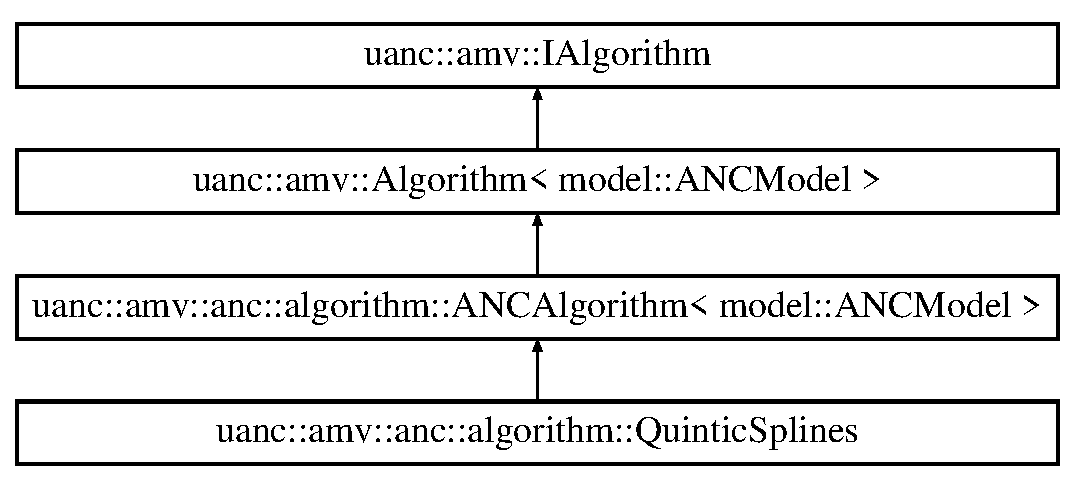
\includegraphics[height=4.000000cm]{classuanc_1_1amv_1_1anc_1_1algorithm_1_1_spline_interpolation}
\end{center}
\end{figure}
\subsection*{Public Member Functions}
\begin{DoxyCompactItemize}
\item 
std\+::string \hyperlink{classuanc_1_1amv_1_1anc_1_1algorithm_1_1_spline_interpolation_a1a26a15fbebb957e8a9b404a19ed41fb}{get\+Name} () final
\begin{DoxyCompactList}\small\item\em Returns the name of the algorithm. \end{DoxyCompactList}\item 
void \hyperlink{classuanc_1_1amv_1_1anc_1_1algorithm_1_1_spline_interpolation_a60dcdd5acbba6fee64cf228485b81523}{invert} (std\+::shared\+\_\+ptr$<$ \hyperlink{classuanc_1_1amv_1_1_inverted_model}{Inverted\+Model} $>$ in) final
\begin{DoxyCompactList}\small\item\em Inverts the input signal. \end{DoxyCompactList}\item 
\hyperlink{classuanc_1_1amv_1_1_algorithm}{Algorithm} $\ast$ \hyperlink{classuanc_1_1amv_1_1anc_1_1algorithm_1_1_spline_interpolation_a43063277ff720c71b932ee29673b568f}{clone} () final
\begin{DoxyCompactList}\small\item\em Clones the current instance. \end{DoxyCompactList}\end{DoxyCompactItemize}
\subsection*{Protected Member Functions}
\begin{DoxyCompactItemize}
\item 
\hyperlink{classuanc_1_1amv_1_1_algorithm_view}{Algorithm\+View}$<$ \hyperlink{classuanc_1_1amv_1_1anc_1_1model_1_1_a_n_c_model}{model\+::\+A\+N\+C\+Model} $>$ $\ast$ \hyperlink{classuanc_1_1amv_1_1anc_1_1algorithm_1_1_spline_interpolation_a93fd1b1f3ac140863f53464eea2820f3}{construct\+View} () final
\begin{DoxyCompactList}\small\item\em Constructs a view, which can handle an A\+N\+C\+Model. \end{DoxyCompactList}\end{DoxyCompactItemize}


\subsection{Member Function Documentation}
\index{uanc\+::amv\+::anc\+::algorithm\+::\+Spline\+Interpolation@{uanc\+::amv\+::anc\+::algorithm\+::\+Spline\+Interpolation}!clone@{clone}}
\index{clone@{clone}!uanc\+::amv\+::anc\+::algorithm\+::\+Spline\+Interpolation@{uanc\+::amv\+::anc\+::algorithm\+::\+Spline\+Interpolation}}
\subsubsection[{\texorpdfstring{clone() final}{clone() final}}]{\setlength{\rightskip}{0pt plus 5cm}{\bf Algorithm}$\ast$ uanc\+::amv\+::anc\+::algorithm\+::\+Spline\+Interpolation\+::clone (
\begin{DoxyParamCaption}
{}
\end{DoxyParamCaption}
)\hspace{0.3cm}{\ttfamily [inline]}, {\ttfamily [final]}, {\ttfamily [virtual]}}\hypertarget{classuanc_1_1amv_1_1anc_1_1algorithm_1_1_spline_interpolation_a43063277ff720c71b932ee29673b568f}{}\label{classuanc_1_1amv_1_1anc_1_1algorithm_1_1_spline_interpolation_a43063277ff720c71b932ee29673b568f}


Clones the current instance. 

This is basically the prototype pattern. It gets used to create an copy of the current \hyperlink{classuanc_1_1amv_1_1anc_1_1algorithm_1_1_inverse_direct_algorithm}{Inverse\+Direct\+Algorithm}. To do so it simply creates a new instance.

\begin{DoxyReturn}{Returns}
The cloned algorithm. 
\end{DoxyReturn}


Implements \hyperlink{classuanc_1_1amv_1_1_i_algorithm_af6fcbfa35f460363c2cc7e6134af8dc7}{uanc\+::amv\+::\+I\+Algorithm}.

\index{uanc\+::amv\+::anc\+::algorithm\+::\+Spline\+Interpolation@{uanc\+::amv\+::anc\+::algorithm\+::\+Spline\+Interpolation}!construct\+View@{construct\+View}}
\index{construct\+View@{construct\+View}!uanc\+::amv\+::anc\+::algorithm\+::\+Spline\+Interpolation@{uanc\+::amv\+::anc\+::algorithm\+::\+Spline\+Interpolation}}
\subsubsection[{\texorpdfstring{construct\+View() final}{constructView() final}}]{\setlength{\rightskip}{0pt plus 5cm}{\bf Algorithm\+View}$<${\bf model\+::\+A\+N\+C\+Model}$>$$\ast$ uanc\+::amv\+::anc\+::algorithm\+::\+Spline\+Interpolation\+::construct\+View (
\begin{DoxyParamCaption}
{}
\end{DoxyParamCaption}
)\hspace{0.3cm}{\ttfamily [inline]}, {\ttfamily [final]}, {\ttfamily [protected]}, {\ttfamily [virtual]}}\hypertarget{classuanc_1_1amv_1_1anc_1_1algorithm_1_1_spline_interpolation_a93fd1b1f3ac140863f53464eea2820f3}{}\label{classuanc_1_1amv_1_1anc_1_1algorithm_1_1_spline_interpolation_a93fd1b1f3ac140863f53464eea2820f3}


Constructs a view, which can handle an A\+N\+C\+Model. 

This view basically display the standard information of the algorithm.

\begin{DoxyReturn}{Returns}
The created A\+N\+C\+View. 
\end{DoxyReturn}


Implements \hyperlink{classuanc_1_1amv_1_1_algorithm_af5561072283ed19634893263c95a4b6e}{uanc\+::amv\+::\+Algorithm$<$ model\+::\+A\+N\+C\+Model $>$}.

\index{uanc\+::amv\+::anc\+::algorithm\+::\+Spline\+Interpolation@{uanc\+::amv\+::anc\+::algorithm\+::\+Spline\+Interpolation}!get\+Name@{get\+Name}}
\index{get\+Name@{get\+Name}!uanc\+::amv\+::anc\+::algorithm\+::\+Spline\+Interpolation@{uanc\+::amv\+::anc\+::algorithm\+::\+Spline\+Interpolation}}
\subsubsection[{\texorpdfstring{get\+Name() final}{getName() final}}]{\setlength{\rightskip}{0pt plus 5cm}std\+::string uanc\+::amv\+::anc\+::algorithm\+::\+Spline\+Interpolation\+::get\+Name (
\begin{DoxyParamCaption}
{}
\end{DoxyParamCaption}
)\hspace{0.3cm}{\ttfamily [inline]}, {\ttfamily [final]}, {\ttfamily [virtual]}}\hypertarget{classuanc_1_1amv_1_1anc_1_1algorithm_1_1_spline_interpolation_a1a26a15fbebb957e8a9b404a19ed41fb}{}\label{classuanc_1_1amv_1_1anc_1_1algorithm_1_1_spline_interpolation_a1a26a15fbebb957e8a9b404a19ed41fb}


Returns the name of the algorithm. 

Simply passes back the name of the algorithm.

\begin{DoxyReturn}{Returns}
Name of the algorithm 
\end{DoxyReturn}


Implements \hyperlink{classuanc_1_1amv_1_1_i_algorithm_a4935ab2fdacccf7df35d6fb596075edb}{uanc\+::amv\+::\+I\+Algorithm}.

\index{uanc\+::amv\+::anc\+::algorithm\+::\+Spline\+Interpolation@{uanc\+::amv\+::anc\+::algorithm\+::\+Spline\+Interpolation}!invert@{invert}}
\index{invert@{invert}!uanc\+::amv\+::anc\+::algorithm\+::\+Spline\+Interpolation@{uanc\+::amv\+::anc\+::algorithm\+::\+Spline\+Interpolation}}
\subsubsection[{\texorpdfstring{invert(std\+::shared\+\_\+ptr$<$ Inverted\+Model $>$ in) final}{invert(std::shared_ptr< InvertedModel > in) final}}]{\setlength{\rightskip}{0pt plus 5cm}void uanc\+::amv\+::anc\+::algorithm\+::\+Spline\+Interpolation\+::invert (
\begin{DoxyParamCaption}
\item[{std\+::shared\+\_\+ptr$<$ {\bf Inverted\+Model} $>$}]{in}
\end{DoxyParamCaption}
)\hspace{0.3cm}{\ttfamily [inline]}, {\ttfamily [final]}, {\ttfamily [virtual]}}\hypertarget{classuanc_1_1amv_1_1anc_1_1algorithm_1_1_spline_interpolation_a60dcdd5acbba6fee64cf228485b81523}{}\label{classuanc_1_1amv_1_1anc_1_1algorithm_1_1_spline_interpolation_a60dcdd5acbba6fee64cf228485b81523}


Inverts the input signal. 

This is actually the heart of an A\+NC algorithm inside of this application. It takes an input model and processes it. Besides it should save its data inside the model using \hyperlink{classuanc_1_1amv_1_1anc_1_1algorithm_1_1_a_n_c_algorithm_a12ce80f6746cbb440cf771fc6878f7cf}{get\+Model()}.


\begin{DoxyParams}{Parameters}
{\em input} & The input model containing the original signal. \\
\hline
\end{DoxyParams}


Implements \hyperlink{classuanc_1_1amv_1_1anc_1_1algorithm_1_1_a_n_c_algorithm_abfdc7f14f7e41e408ee08037a839760d}{uanc\+::amv\+::anc\+::algorithm\+::\+A\+N\+C\+Algorithm$<$ model\+::\+A\+N\+C\+Model $>$}.



The documentation for this class was generated from the following file\+:\begin{DoxyCompactItemize}
\item 
/home/kurt/\+Documents/\+Studium/\+Bachelor\+\_\+\+Praktikum/\+U\+A\+N\+C/\+Code/\+U\+A\+N\+C/amv/anc/algorithm/\hyperlink{_spline_interpolation_8h}{Spline\+Interpolation.\+h}\end{DoxyCompactItemize}

\hypertarget{classuanc_1_1amv_1_1signal_1_1_transformation_algorithm_register}{}\section{uanc\+:\+:amv\+:\+:signal\+:\+:Transformation\+Algorithm\+Register Class Reference}
\label{classuanc_1_1amv_1_1signal_1_1_transformation_algorithm_register}\index{uanc\+::amv\+::signal\+::\+Transformation\+Algorithm\+Register@{uanc\+::amv\+::signal\+::\+Transformation\+Algorithm\+Register}}


This class is used to retain a list of all transformation.  




{\ttfamily \#include $<$Transformation\+Algorithm\+Register.\+h$>$}

\subsection*{Static Public Member Functions}
\begin{DoxyCompactItemize}
\item 
static std\+::shared\+\_\+ptr$<$ std\+::vector$<$ \hyperlink{classuanc_1_1amv_1_1_i_algorithm}{uanc\+::amv\+::\+I\+Algorithm} $\ast$ $>$ $>$ \hyperlink{classuanc_1_1amv_1_1signal_1_1_transformation_algorithm_register_ad03dc4e23a840670d57ef3d6d1bfb4b9}{get\+Transformations} ()
\begin{DoxyCompactList}\small\item\em Supply all registered transformation. \end{DoxyCompactList}\end{DoxyCompactItemize}


\subsection{Detailed Description}
This class is used to retain a list of all transformation. 

This class represents the extendability point for all transformations and data representations If you have implemented another representation simply register it inside of this class and it will automatically be integrated in the application. 

\subsection{Member Function Documentation}
\index{uanc\+::amv\+::signal\+::\+Transformation\+Algorithm\+Register@{uanc\+::amv\+::signal\+::\+Transformation\+Algorithm\+Register}!get\+Transformations@{get\+Transformations}}
\index{get\+Transformations@{get\+Transformations}!uanc\+::amv\+::signal\+::\+Transformation\+Algorithm\+Register@{uanc\+::amv\+::signal\+::\+Transformation\+Algorithm\+Register}}
\subsubsection[{\texorpdfstring{get\+Transformations()}{getTransformations()}}]{\setlength{\rightskip}{0pt plus 5cm}static std\+::shared\+\_\+ptr$<$std\+::vector$<${\bf uanc\+::amv\+::\+I\+Algorithm} $\ast$$>$ $>$ uanc\+::amv\+::signal\+::\+Transformation\+Algorithm\+Register\+::get\+Transformations (
\begin{DoxyParamCaption}
{}
\end{DoxyParamCaption}
)\hspace{0.3cm}{\ttfamily [inline]}, {\ttfamily [static]}}\hypertarget{classuanc_1_1amv_1_1signal_1_1_transformation_algorithm_register_ad03dc4e23a840670d57ef3d6d1bfb4b9}{}\label{classuanc_1_1amv_1_1signal_1_1_transformation_algorithm_register_ad03dc4e23a840670d57ef3d6d1bfb4b9}


Supply all registered transformation. 

This method basically returns a list of all transformations registered inside of the application. To add you new implemented one, simply add it to the list at the bottom.

\begin{DoxyReturn}{Returns}
A vector containing a prototype of all transformations. 
\end{DoxyReturn}


The documentation for this class was generated from the following file\+:\begin{DoxyCompactItemize}
\item 
/home/kurt/\+Documents/\+Studium/\+Bachelor\+\_\+\+Praktikum/\+U\+A\+N\+C/\+Code/\+U\+A\+N\+C/amv/signal/\hyperlink{_transformation_algorithm_register_8h}{Transformation\+Algorithm\+Register.\+h}\end{DoxyCompactItemize}

\chapter{File Documentation}
\hypertarget{_algorithm_8h}{}\section{/ext/local/\+University/\+B\+P/\+Git/\+U\+A\+N\+C/\+Code/\+U\+A\+N\+C/amv/\+Algorithm.h File Reference}
\label{_algorithm_8h}\index{/ext/local/\+University/\+B\+P/\+Git/\+U\+A\+N\+C/\+Code/\+U\+A\+N\+C/amv/\+Algorithm.\+h@{/ext/local/\+University/\+B\+P/\+Git/\+U\+A\+N\+C/\+Code/\+U\+A\+N\+C/amv/\+Algorithm.\+h}}
{\ttfamily \#include \char`\"{}I\+Algorithm.\+h\char`\"{}}\\*
{\ttfamily \#include \char`\"{}Algorithm\+View.\+h\char`\"{}}\\*
\subsection*{Classes}
\begin{DoxyCompactItemize}
\item 
class \hyperlink{classuanc_1_1amv_1_1_algorithm}{uanc\+::amv\+::\+Algorithm$<$ outmodel $>$}
\begin{DoxyCompactList}\small\item\em This is an algorithm used for defining more specific algorithms. \end{DoxyCompactList}\end{DoxyCompactItemize}
\subsection*{Namespaces}
\begin{DoxyCompactItemize}
\item 
 \hyperlink{namespaceuanc}{uanc}
\item 
 \hyperlink{namespaceuanc_1_1amv}{uanc\+::amv}
\end{DoxyCompactItemize}

\hypertarget{_algorithm_thread_8h}{}\section{/ext/local/\+University/\+B\+P/\+Git/\+U\+A\+N\+C/\+Code/\+U\+A\+N\+C/amv/\+Algorithm\+Thread.h File Reference}
\label{_algorithm_thread_8h}\index{/ext/local/\+University/\+B\+P/\+Git/\+U\+A\+N\+C/\+Code/\+U\+A\+N\+C/amv/\+Algorithm\+Thread.\+h@{/ext/local/\+University/\+B\+P/\+Git/\+U\+A\+N\+C/\+Code/\+U\+A\+N\+C/amv/\+Algorithm\+Thread.\+h}}
{\ttfamily \#include $<$Q\+Thread$>$}\\*
{\ttfamily \#include \char`\"{}I\+Algorithm.\+h\char`\"{}}\\*
\subsection*{Classes}
\begin{DoxyCompactItemize}
\item 
class \hyperlink{classuanc_1_1amv_1_1_algorithm_thread}{uanc\+::amv\+::\+Algorithm\+Thread}
\end{DoxyCompactItemize}
\subsection*{Namespaces}
\begin{DoxyCompactItemize}
\item 
 \hyperlink{namespaceuanc}{uanc}
\item 
 \hyperlink{namespaceuanc_1_1amv}{uanc\+::amv}
\end{DoxyCompactItemize}

\hypertarget{_algorithm_view_8h}{}\section{/home/kurt/\+Documents/\+Studium/\+Bachelor\+\_\+\+Praktikum/\+U\+A\+N\+C/\+Code/\+U\+A\+N\+C/amv/\+Algorithm\+View.h File Reference}
\label{_algorithm_view_8h}\index{/home/kurt/\+Documents/\+Studium/\+Bachelor\+\_\+\+Praktikum/\+U\+A\+N\+C/\+Code/\+U\+A\+N\+C/amv/\+Algorithm\+View.\+h@{/home/kurt/\+Documents/\+Studium/\+Bachelor\+\_\+\+Praktikum/\+U\+A\+N\+C/\+Code/\+U\+A\+N\+C/amv/\+Algorithm\+View.\+h}}
{\ttfamily \#include \char`\"{}I\+Algorithm\+View.\+h\char`\"{}}\\*
\subsection*{Classes}
\begin{DoxyCompactItemize}
\item 
class \hyperlink{classuanc_1_1amv_1_1_algorithm_view}{uanc\+::amv\+::\+Algorithm\+View$<$ inmodel $>$}
\begin{DoxyCompactList}\small\item\em Basic algorithm associated view. \end{DoxyCompactList}\end{DoxyCompactItemize}
\subsection*{Namespaces}
\begin{DoxyCompactItemize}
\item 
 \hyperlink{namespaceuanc}{uanc}
\item 
 \hyperlink{namespaceuanc_1_1amv}{uanc\+::amv}
\end{DoxyCompactItemize}

\hypertarget{_a_n_c_algorithm_8h}{}\section{/ext/local/\+University/\+B\+P/\+Git/\+U\+A\+N\+C/\+Code/\+U\+A\+N\+C/amv/anc/algorithm/\+A\+N\+C\+Algorithm.h File Reference}
\label{_a_n_c_algorithm_8h}\index{/ext/local/\+University/\+B\+P/\+Git/\+U\+A\+N\+C/\+Code/\+U\+A\+N\+C/amv/anc/algorithm/\+A\+N\+C\+Algorithm.\+h@{/ext/local/\+University/\+B\+P/\+Git/\+U\+A\+N\+C/\+Code/\+U\+A\+N\+C/amv/anc/algorithm/\+A\+N\+C\+Algorithm.\+h}}
{\ttfamily \#include $<$Code/\+U\+A\+N\+C/amv/\+Algorithm.\+h$>$}\\*
\subsection*{Classes}
\begin{DoxyCompactItemize}
\item 
class \hyperlink{classuanc_1_1amv_1_1anc_1_1algorithm_1_1_a_n_c_algorithm}{uanc\+::amv\+::anc\+::algorithm\+::\+A\+N\+C\+Algorithm$<$ datamodel, viewmodel $>$}
\begin{DoxyCompactList}\small\item\em Every algorithm used inside has to be derived by this class. \end{DoxyCompactList}\end{DoxyCompactItemize}
\subsection*{Namespaces}
\begin{DoxyCompactItemize}
\item 
 \hyperlink{namespaceuanc}{uanc}
\item 
 \hyperlink{namespaceuanc_1_1amv}{uanc\+::amv}
\item 
 \hyperlink{namespaceuanc_1_1amv_1_1anc}{uanc\+::amv\+::anc}
\item 
 \hyperlink{namespaceuanc_1_1amv_1_1anc_1_1algorithm}{uanc\+::amv\+::anc\+::algorithm}
\end{DoxyCompactItemize}

\hypertarget{_inverse_direct_algorithm_8h}{}\section{/home/kurt/\+Documents/\+Studium/\+Bachelor\+\_\+\+Praktikum/\+U\+A\+N\+C/\+Code/\+U\+A\+N\+C/amv/anc/algorithm/\+Inverse\+Direct\+Algorithm.h File Reference}
\label{_inverse_direct_algorithm_8h}\index{/home/kurt/\+Documents/\+Studium/\+Bachelor\+\_\+\+Praktikum/\+U\+A\+N\+C/\+Code/\+U\+A\+N\+C/amv/anc/algorithm/\+Inverse\+Direct\+Algorithm.\+h@{/home/kurt/\+Documents/\+Studium/\+Bachelor\+\_\+\+Praktikum/\+U\+A\+N\+C/\+Code/\+U\+A\+N\+C/amv/anc/algorithm/\+Inverse\+Direct\+Algorithm.\+h}}
{\ttfamily \#include $<$Code/\+U\+A\+N\+C/amv/anc/model/\+A\+N\+C\+Model.\+h$>$}\\*
{\ttfamily \#include $<$Code/\+U\+A\+N\+C/amv/anc/view/\+A\+N\+C\+View.\+h$>$}\\*
{\ttfamily \#include $<$Code/\+U\+A\+N\+C/amv/anc/view/\+P\+M\+View.\+h$>$}\\*
{\ttfamily \#include $<$Code/\+U\+A\+N\+C/util/\+Performance\+Measure.\+h$>$}\\*
{\ttfamily \#include \char`\"{}A\+N\+C\+Algorithm.\+h\char`\"{}}\\*
\subsection*{Classes}
\begin{DoxyCompactItemize}
\item 
class \hyperlink{classuanc_1_1amv_1_1anc_1_1algorithm_1_1_inverse_direct_algorithm}{uanc\+::amv\+::anc\+::algorithm\+::\+Inverse\+Direct\+Algorithm}
\begin{DoxyCompactList}\small\item\em Direct inversion algorithm. \end{DoxyCompactList}\end{DoxyCompactItemize}
\subsection*{Namespaces}
\begin{DoxyCompactItemize}
\item 
 \hyperlink{namespaceuanc}{uanc}
\item 
 \hyperlink{namespaceuanc_1_1amv}{uanc\+::amv}
\item 
 \hyperlink{namespaceuanc_1_1amv_1_1anc}{uanc\+::amv\+::anc}
\item 
 \hyperlink{namespaceuanc_1_1amv_1_1anc_1_1algorithm}{uanc\+::amv\+::anc\+::algorithm}
\end{DoxyCompactItemize}

\hypertarget{_inverse_f_f_t_algorithm_8h}{}\section{/home/kurt/\+Documents/\+Studium/\+Bachelor\+\_\+\+Praktikum/\+U\+A\+N\+C/\+Code/\+U\+A\+N\+C/amv/anc/algorithm/\+Inverse\+F\+F\+T\+Algorithm.h File Reference}
\label{_inverse_f_f_t_algorithm_8h}\index{/home/kurt/\+Documents/\+Studium/\+Bachelor\+\_\+\+Praktikum/\+U\+A\+N\+C/\+Code/\+U\+A\+N\+C/amv/anc/algorithm/\+Inverse\+F\+F\+T\+Algorithm.\+h@{/home/kurt/\+Documents/\+Studium/\+Bachelor\+\_\+\+Praktikum/\+U\+A\+N\+C/\+Code/\+U\+A\+N\+C/amv/anc/algorithm/\+Inverse\+F\+F\+T\+Algorithm.\+h}}
{\ttfamily \#include $<$complex$>$}\\*
{\ttfamily \#include $<$Code/libs/aquila/source/\+Signal\+Source.\+h$>$}\\*
{\ttfamily \#include $<$Code/libs/aquila/transform/\+Fft\+Factory.\+h$>$}\\*
{\ttfamily \#include $<$Code/\+U\+A\+N\+C/amv/anc/model/\+A\+N\+C\+Model.\+h$>$}\\*
{\ttfamily \#include $<$Code/\+U\+A\+N\+C/amv/anc/view/\+A\+N\+C\+View.\+h$>$}\\*
{\ttfamily \#include $<$Code/\+U\+A\+N\+C/util/\+Performance\+Measure.\+h$>$}\\*
{\ttfamily \#include $<$Code/\+U\+A\+N\+C/amv/anc/view/\+P\+M\+View.\+h$>$}\\*
{\ttfamily \#include \char`\"{}A\+N\+C\+Algorithm.\+h\char`\"{}}\\*
\subsection*{Classes}
\begin{DoxyCompactItemize}
\item 
class \hyperlink{classuanc_1_1amv_1_1anc_1_1algorithm_1_1_inverse_f_f_t_algorithm}{uanc\+::amv\+::anc\+::algorithm\+::\+Inverse\+F\+F\+T\+Algorithm}
\begin{DoxyCompactList}\small\item\em F\+FT inversion algorithm. \end{DoxyCompactList}\end{DoxyCompactItemize}
\subsection*{Namespaces}
\begin{DoxyCompactItemize}
\item 
 \hyperlink{namespaceuanc}{uanc}
\item 
 \hyperlink{namespaceuanc_1_1amv}{uanc\+::amv}
\item 
 \hyperlink{namespaceuanc_1_1amv_1_1anc}{uanc\+::amv\+::anc}
\item 
 \hyperlink{namespaceuanc_1_1amv_1_1anc_1_1algorithm}{uanc\+::amv\+::anc\+::algorithm}
\end{DoxyCompactItemize}

\hypertarget{_linear_extrapolation_8h}{}\section{/home/kurt/\+Documents/\+Studium/\+Bachelor\+\_\+\+Praktikum/\+U\+A\+N\+C/\+Code/\+U\+A\+N\+C/amv/anc/algorithm/\+Linear\+Extrapolation.h File Reference}
\label{_linear_extrapolation_8h}\index{/home/kurt/\+Documents/\+Studium/\+Bachelor\+\_\+\+Praktikum/\+U\+A\+N\+C/\+Code/\+U\+A\+N\+C/amv/anc/algorithm/\+Linear\+Extrapolation.\+h@{/home/kurt/\+Documents/\+Studium/\+Bachelor\+\_\+\+Praktikum/\+U\+A\+N\+C/\+Code/\+U\+A\+N\+C/amv/anc/algorithm/\+Linear\+Extrapolation.\+h}}
\subsection*{Classes}
\begin{DoxyCompactItemize}
\item 
class \hyperlink{classuanc_1_1amv_1_1anc_1_1algorithm_1_1_linear_extrapolation}{uanc\+::amv\+::anc\+::algorithm\+::\+Linear\+Extrapolation}
\end{DoxyCompactItemize}
\subsection*{Namespaces}
\begin{DoxyCompactItemize}
\item 
 \hyperlink{namespaceuanc}{uanc}
\item 
 \hyperlink{namespaceuanc_1_1amv}{uanc\+::amv}
\item 
 \hyperlink{namespaceuanc_1_1amv_1_1anc}{uanc\+::amv\+::anc}
\item 
 \hyperlink{namespaceuanc_1_1amv_1_1anc_1_1algorithm}{uanc\+::amv\+::anc\+::algorithm}
\end{DoxyCompactItemize}

\hypertarget{_spline_interpolation_8h}{}\section{/home/kurt/\+Documents/\+Studium/\+Bachelor\+\_\+\+Praktikum/\+U\+A\+N\+C/\+Code/\+U\+A\+N\+C/amv/anc/algorithm/\+Spline\+Interpolation.h File Reference}
\label{_spline_interpolation_8h}\index{/home/kurt/\+Documents/\+Studium/\+Bachelor\+\_\+\+Praktikum/\+U\+A\+N\+C/\+Code/\+U\+A\+N\+C/amv/anc/algorithm/\+Spline\+Interpolation.\+h@{/home/kurt/\+Documents/\+Studium/\+Bachelor\+\_\+\+Praktikum/\+U\+A\+N\+C/\+Code/\+U\+A\+N\+C/amv/anc/algorithm/\+Spline\+Interpolation.\+h}}
{\ttfamily \#include $<$Code/\+U\+A\+N\+C/amv/anc/model/\+A\+N\+C\+Model.\+h$>$}\\*
{\ttfamily \#include $<$Code/\+U\+A\+N\+C/amv/\+Algorithm.\+h$>$}\\*
{\ttfamily \#include $<$Code/\+U\+A\+N\+C/amv/anc/view/\+P\+M\+View.\+h$>$}\\*
{\ttfamily \#include $<$armadillo$>$}\\*
{\ttfamily \#include $<$list$>$}\\*
{\ttfamily \#include \char`\"{}A\+N\+C\+Algorithm.\+h\char`\"{}}\\*
\subsection*{Classes}
\begin{DoxyCompactItemize}
\item 
class \hyperlink{classuanc_1_1amv_1_1anc_1_1algorithm_1_1_spline_interpolation}{uanc\+::amv\+::anc\+::algorithm\+::\+Spline\+Interpolation}
\end{DoxyCompactItemize}
\subsection*{Namespaces}
\begin{DoxyCompactItemize}
\item 
 \hyperlink{namespaceuanc}{uanc}
\item 
 \hyperlink{namespaceuanc_1_1amv}{uanc\+::amv}
\item 
 \hyperlink{namespaceuanc_1_1amv_1_1anc}{uanc\+::amv\+::anc}
\item 
 \hyperlink{namespaceuanc_1_1amv_1_1anc_1_1algorithm}{uanc\+::amv\+::anc\+::algorithm}
\end{DoxyCompactItemize}

\hypertarget{_a_n_c_algorithm_register_8h}{}\section{/home/kurt/\+Documents/\+Studium/\+Bachelor\+\_\+\+Praktikum/\+U\+A\+N\+C/\+Code/\+U\+A\+N\+C/amv/anc/\+A\+N\+C\+Algorithm\+Register.h File Reference}
\label{_a_n_c_algorithm_register_8h}\index{/home/kurt/\+Documents/\+Studium/\+Bachelor\+\_\+\+Praktikum/\+U\+A\+N\+C/\+Code/\+U\+A\+N\+C/amv/anc/\+A\+N\+C\+Algorithm\+Register.\+h@{/home/kurt/\+Documents/\+Studium/\+Bachelor\+\_\+\+Praktikum/\+U\+A\+N\+C/\+Code/\+U\+A\+N\+C/amv/anc/\+A\+N\+C\+Algorithm\+Register.\+h}}
{\ttfamily \#include $<$memory$>$}\\*
{\ttfamily \#include \char`\"{}Code/\+U\+A\+N\+C/amv/anc/algorithm/\+Inverse\+Direct\+Algorithm.\+h\char`\"{}}\\*
{\ttfamily \#include \char`\"{}Code/\+U\+A\+N\+C/amv/anc/algorithm/\+Inverse\+F\+F\+T\+Algorithm.\+h\char`\"{}}\\*
{\ttfamily \#include \char`\"{}Code/\+U\+A\+N\+C/amv/anc/algorithm/\+Linear\+Extrapolation.\+h\char`\"{}}\\*
{\ttfamily \#include \char`\"{}Code/\+U\+A\+N\+C/amv/anc/algorithm/\+Locally\+Weighted\+Regression.\+h\char`\"{}}\\*
{\ttfamily \#include \char`\"{}Code/\+U\+A\+N\+C/amv/anc/algorithm/\+Quintic\+Splines.\+h\char`\"{}}\\*
{\ttfamily \#include \char`\"{}Code/\+U\+A\+N\+C/amv/anc/algorithm/\+Polynomial\+Regression.\+h\char`\"{}}\\*
\subsection*{Classes}
\begin{DoxyCompactItemize}
\item 
class \hyperlink{classuanc_1_1amv_1_1anc_1_1_a_n_c_algorithm_register}{uanc\+::amv\+::anc\+::\+A\+N\+C\+Algorithm\+Register}
\begin{DoxyCompactList}\small\item\em This class is used to retain a list of all algorithms. \end{DoxyCompactList}\end{DoxyCompactItemize}
\subsection*{Namespaces}
\begin{DoxyCompactItemize}
\item 
 \hyperlink{namespaceuanc}{uanc}
\item 
 \hyperlink{namespaceuanc_1_1amv}{uanc\+::amv}
\item 
 \hyperlink{namespaceuanc_1_1amv_1_1anc}{uanc\+::amv\+::anc}
\end{DoxyCompactItemize}

\hypertarget{_a_n_c_model_8h}{}\section{/ext/local/\+University/\+B\+P/\+Git/\+U\+A\+N\+C/\+Code/\+U\+A\+N\+C/amv/anc/model/\+A\+N\+C\+Model.h File Reference}
\label{_a_n_c_model_8h}\index{/ext/local/\+University/\+B\+P/\+Git/\+U\+A\+N\+C/\+Code/\+U\+A\+N\+C/amv/anc/model/\+A\+N\+C\+Model.\+h@{/ext/local/\+University/\+B\+P/\+Git/\+U\+A\+N\+C/\+Code/\+U\+A\+N\+C/amv/anc/model/\+A\+N\+C\+Model.\+h}}
{\ttfamily \#include $<$Code/\+U\+A\+N\+C/amv/\+Inverted\+Model.\+h$>$}\\*
{\ttfamily \#include $<$memory$>$}\\*
{\ttfamily \#include $<$Code/\+U\+A\+N\+C/util/\+Performance\+Measure.\+h$>$}\\*
\subsection*{Classes}
\begin{DoxyCompactItemize}
\item 
class \hyperlink{classuanc_1_1amv_1_1anc_1_1model_1_1_a_n_c_model}{uanc\+::amv\+::anc\+::model\+::\+A\+N\+C\+Model}
\begin{DoxyCompactList}\small\item\em This is an \hyperlink{classuanc_1_1amv_1_1anc_1_1model_1_1_a_n_c_model}{A\+N\+C\+Model}. \end{DoxyCompactList}\end{DoxyCompactItemize}
\subsection*{Namespaces}
\begin{DoxyCompactItemize}
\item 
 \hyperlink{namespaceuanc}{uanc}
\item 
 \hyperlink{namespaceuanc_1_1amv}{uanc\+::amv}
\item 
 \hyperlink{namespaceuanc_1_1amv_1_1anc}{uanc\+::amv\+::anc}
\item 
 \hyperlink{namespaceuanc_1_1amv_1_1anc_1_1model}{uanc\+::amv\+::anc\+::model}
\end{DoxyCompactItemize}

\hypertarget{_a_n_c_view_8cpp}{}\section{/ext/local/\+University/\+B\+P/\+Git/\+U\+A\+N\+C/\+Code/\+U\+A\+N\+C/amv/anc/view/\+A\+N\+C\+View.cpp File Reference}
\label{_a_n_c_view_8cpp}\index{/ext/local/\+University/\+B\+P/\+Git/\+U\+A\+N\+C/\+Code/\+U\+A\+N\+C/amv/anc/view/\+A\+N\+C\+View.\+cpp@{/ext/local/\+University/\+B\+P/\+Git/\+U\+A\+N\+C/\+Code/\+U\+A\+N\+C/amv/anc/view/\+A\+N\+C\+View.\+cpp}}
{\ttfamily \#include $<$Code/\+U\+A\+N\+C/gui/\+Plot\+Widget.\+h$>$}\\*
{\ttfamily \#include \char`\"{}A\+N\+C\+View.\+h\char`\"{}}\\*
\subsection*{Namespaces}
\begin{DoxyCompactItemize}
\item 
 \hyperlink{namespaceuanc}{uanc}
\item 
 \hyperlink{namespaceuanc_1_1amv}{uanc\+::amv}
\item 
 \hyperlink{namespaceuanc_1_1amv_1_1anc}{uanc\+::amv\+::anc}
\item 
 \hyperlink{namespaceuanc_1_1amv_1_1anc_1_1view}{uanc\+::amv\+::anc\+::view}
\end{DoxyCompactItemize}

\hypertarget{_a_n_c_view_8h}{}\section{/ext/local/\+University/\+B\+P/\+Git/\+U\+A\+N\+C/\+Code/\+U\+A\+N\+C/amv/anc/view/\+A\+N\+C\+View.h File Reference}
\label{_a_n_c_view_8h}\index{/ext/local/\+University/\+B\+P/\+Git/\+U\+A\+N\+C/\+Code/\+U\+A\+N\+C/amv/anc/view/\+A\+N\+C\+View.\+h@{/ext/local/\+University/\+B\+P/\+Git/\+U\+A\+N\+C/\+Code/\+U\+A\+N\+C/amv/anc/view/\+A\+N\+C\+View.\+h}}
{\ttfamily \#include $<$memory$>$}\\*
{\ttfamily \#include $<$Qt\+Widgets/\+Q\+Widget$>$}\\*
{\ttfamily \#include $<$Code/\+U\+A\+N\+C/amv/\+Inverted\+Model.\+h$>$}\\*
{\ttfamily \#include $<$Code/\+U\+A\+N\+C/amv/\+Algorithm\+View.\+h$>$}\\*
{\ttfamily \#include $<$Code/\+U\+A\+N\+C/util/tools/\+Path.\+h$>$}\\*
{\ttfamily \#include $<$Code/\+U\+A\+N\+C/gui/\+Plot\+Widget.\+h$>$}\\*
{\ttfamily \#include $<$Code/\+U\+A\+N\+C/amv/anc/model/\+A\+N\+C\+Model.\+h$>$}\\*
\subsection*{Classes}
\begin{DoxyCompactItemize}
\item 
class \hyperlink{classuanc_1_1amv_1_1anc_1_1view_1_1_a_n_c_view}{uanc\+::amv\+::anc\+::view\+::\+A\+N\+C\+View}
\begin{DoxyCompactList}\small\item\em Represents an \hyperlink{classuanc_1_1amv_1_1anc_1_1view_1_1_a_n_c_view}{A\+N\+C\+View}. \end{DoxyCompactList}\end{DoxyCompactItemize}
\subsection*{Namespaces}
\begin{DoxyCompactItemize}
\item 
 \hyperlink{namespaceuanc}{uanc}
\item 
 \hyperlink{namespaceuanc_1_1amv}{uanc\+::amv}
\item 
 \hyperlink{namespaceuanc_1_1amv_1_1anc}{uanc\+::amv\+::anc}
\item 
 \hyperlink{namespaceuanc_1_1amv_1_1anc_1_1view}{uanc\+::amv\+::anc\+::view}
\end{DoxyCompactItemize}

\hypertarget{_p_m_view_8cpp}{}\section{/ext/local/\+University/\+B\+P/\+Git/\+U\+A\+N\+C/\+Code/\+U\+A\+N\+C/amv/anc/view/\+P\+M\+View.cpp File Reference}
\label{_p_m_view_8cpp}\index{/ext/local/\+University/\+B\+P/\+Git/\+U\+A\+N\+C/\+Code/\+U\+A\+N\+C/amv/anc/view/\+P\+M\+View.\+cpp@{/ext/local/\+University/\+B\+P/\+Git/\+U\+A\+N\+C/\+Code/\+U\+A\+N\+C/amv/anc/view/\+P\+M\+View.\+cpp}}
{\ttfamily \#include $<$Code/\+U\+A\+N\+C/gui/\+Plot\+Widget.\+h$>$}\\*
{\ttfamily \#include $<$Code/\+U\+A\+N\+C/gui/\+P\+M\+Widget.\+h$>$}\\*
{\ttfamily \#include \char`\"{}P\+M\+View.\+h\char`\"{}}\\*
{\ttfamily \#include \char`\"{}Code/\+U\+A\+N\+C/util/\+Global\+Settings.\+h\char`\"{}}\\*
\subsection*{Namespaces}
\begin{DoxyCompactItemize}
\item 
 \hyperlink{namespaceuanc}{uanc}
\item 
 \hyperlink{namespaceuanc_1_1amv}{uanc\+::amv}
\item 
 \hyperlink{namespaceuanc_1_1amv_1_1anc}{uanc\+::amv\+::anc}
\item 
 \hyperlink{namespaceuanc_1_1amv_1_1anc_1_1view}{uanc\+::amv\+::anc\+::view}
\end{DoxyCompactItemize}

\hypertarget{_p_m_view_8h}{}\section{/ext/local/\+University/\+B\+P/\+Git/\+U\+A\+N\+C/\+Code/\+U\+A\+N\+C/amv/anc/view/\+P\+M\+View.h File Reference}
\label{_p_m_view_8h}\index{/ext/local/\+University/\+B\+P/\+Git/\+U\+A\+N\+C/\+Code/\+U\+A\+N\+C/amv/anc/view/\+P\+M\+View.\+h@{/ext/local/\+University/\+B\+P/\+Git/\+U\+A\+N\+C/\+Code/\+U\+A\+N\+C/amv/anc/view/\+P\+M\+View.\+h}}
{\ttfamily \#include $<$memory$>$}\\*
{\ttfamily \#include $<$Qt\+Widgets/\+Q\+Widget$>$}\\*
{\ttfamily \#include $<$Code/\+U\+A\+N\+C/amv/\+Inverted\+Model.\+h$>$}\\*
{\ttfamily \#include $<$Code/\+U\+A\+N\+C/amv/\+Algorithm\+View.\+h$>$}\\*
{\ttfamily \#include $<$Code/\+U\+A\+N\+C/util/tools/\+Path.\+h$>$}\\*
{\ttfamily \#include $<$Code/\+U\+A\+N\+C/gui/\+P\+M\+Widget.\+h$>$}\\*
{\ttfamily \#include $<$Code/\+U\+A\+N\+C/amv/anc/model/\+A\+N\+C\+Model.\+h$>$}\\*
{\ttfamily \#include $<$Code/\+U\+A\+N\+C/gui/\+Signal\+View\+Widget.\+h$>$}\\*
\subsection*{Classes}
\begin{DoxyCompactItemize}
\item 
class \hyperlink{classuanc_1_1amv_1_1anc_1_1view_1_1_p_m_view}{uanc\+::amv\+::anc\+::view\+::\+P\+M\+View}
\begin{DoxyCompactList}\small\item\em Represents an \hyperlink{classuanc_1_1amv_1_1anc_1_1view_1_1_p_m_view}{P\+M\+View}. \end{DoxyCompactList}\end{DoxyCompactItemize}
\subsection*{Namespaces}
\begin{DoxyCompactItemize}
\item 
 \hyperlink{namespaceuanc}{uanc}
\item 
 \hyperlink{namespaceuanc_1_1amv}{uanc\+::amv}
\item 
 \hyperlink{namespaceuanc_1_1amv_1_1anc}{uanc\+::amv\+::anc}
\item 
 \hyperlink{namespaceuanc_1_1amv_1_1anc_1_1view}{uanc\+::amv\+::anc\+::view}
\end{DoxyCompactItemize}

\hypertarget{_i_algorithm_8h}{}\section{/home/kurt/\+Documents/\+Studium/\+Bachelor\+\_\+\+Praktikum/\+U\+A\+N\+C/\+Code/\+U\+A\+N\+C/amv/\+I\+Algorithm.h File Reference}
\label{_i_algorithm_8h}\index{/home/kurt/\+Documents/\+Studium/\+Bachelor\+\_\+\+Praktikum/\+U\+A\+N\+C/\+Code/\+U\+A\+N\+C/amv/\+I\+Algorithm.\+h@{/home/kurt/\+Documents/\+Studium/\+Bachelor\+\_\+\+Praktikum/\+U\+A\+N\+C/\+Code/\+U\+A\+N\+C/amv/\+I\+Algorithm.\+h}}
{\ttfamily \#include $<$Code/\+U\+A\+N\+C/amv/anc/model/\+A\+N\+C\+Model.\+h$>$}\\*
{\ttfamily \#include \char`\"{}I\+Algorithm\+View.\+h\char`\"{}}\\*
\subsection*{Classes}
\begin{DoxyCompactItemize}
\item 
class \hyperlink{classuanc_1_1amv_1_1_i_algorithm}{uanc\+::amv\+::\+I\+Algorithm}
\begin{DoxyCompactList}\small\item\em General interface for any algorithm. \end{DoxyCompactList}\end{DoxyCompactItemize}
\subsection*{Namespaces}
\begin{DoxyCompactItemize}
\item 
 \hyperlink{namespaceuanc}{uanc}
\item 
 \hyperlink{namespaceuanc_1_1amv}{uanc\+::amv}
\end{DoxyCompactItemize}

\hypertarget{_i_algorithm_view_8h}{}\section{/ext/local/\+University/\+B\+P/\+Git/\+U\+A\+N\+C/\+Code/\+U\+A\+N\+C/amv/\+I\+Algorithm\+View.h File Reference}
\label{_i_algorithm_view_8h}\index{/ext/local/\+University/\+B\+P/\+Git/\+U\+A\+N\+C/\+Code/\+U\+A\+N\+C/amv/\+I\+Algorithm\+View.\+h@{/ext/local/\+University/\+B\+P/\+Git/\+U\+A\+N\+C/\+Code/\+U\+A\+N\+C/amv/\+I\+Algorithm\+View.\+h}}
{\ttfamily \#include $<$Qt\+Widgets/\+Q\+Widget$>$}\\*
\subsection*{Classes}
\begin{DoxyCompactItemize}
\item 
class \hyperlink{classuanc_1_1amv_1_1_i_algorithm_view}{uanc\+::amv\+::\+I\+Algorithm\+View}
\begin{DoxyCompactList}\small\item\em The general interface for every view. \end{DoxyCompactList}\end{DoxyCompactItemize}
\subsection*{Namespaces}
\begin{DoxyCompactItemize}
\item 
 \hyperlink{namespaceuanc}{uanc}
\item 
 \hyperlink{namespaceuanc_1_1amv}{uanc\+::amv}
\end{DoxyCompactItemize}

\hypertarget{_inverted_model_8h}{}\section{/ext/local/\+University/\+B\+P/\+Git/\+U\+A\+N\+C/\+Code/\+U\+A\+N\+C/amv/\+Inverted\+Model.h File Reference}
\label{_inverted_model_8h}\index{/ext/local/\+University/\+B\+P/\+Git/\+U\+A\+N\+C/\+Code/\+U\+A\+N\+C/amv/\+Inverted\+Model.\+h@{/ext/local/\+University/\+B\+P/\+Git/\+U\+A\+N\+C/\+Code/\+U\+A\+N\+C/amv/\+Inverted\+Model.\+h}}
{\ttfamily \#include $<$Code/\+U\+A\+N\+C/amv/\+Signal\+Model.\+h$>$}\\*
{\ttfamily \#include $<$memory$>$}\\*
{\ttfamily \#include $<$Code/\+U\+A\+N\+C/util/\+Performance\+Measure.\+h$>$}\\*
\subsection*{Classes}
\begin{DoxyCompactItemize}
\item 
class \hyperlink{classuanc_1_1amv_1_1_inverted_model}{uanc\+::amv\+::\+Inverted\+Model}
\begin{DoxyCompactList}\small\item\em This is an \hyperlink{classuanc_1_1amv_1_1_inverted_model}{Inverted\+Model}. \end{DoxyCompactList}\end{DoxyCompactItemize}
\subsection*{Namespaces}
\begin{DoxyCompactItemize}
\item 
 \hyperlink{namespaceuanc}{uanc}
\item 
 \hyperlink{namespaceuanc_1_1amv}{uanc\+::amv}
\end{DoxyCompactItemize}

\hypertarget{_performance_measurement_register_8cpp}{}\section{/ext/local/\+University/\+B\+P/\+Git/\+U\+A\+N\+C/\+Code/\+U\+A\+N\+C/amv/\+Performance\+Measurement\+Register.cpp File Reference}
\label{_performance_measurement_register_8cpp}\index{/ext/local/\+University/\+B\+P/\+Git/\+U\+A\+N\+C/\+Code/\+U\+A\+N\+C/amv/\+Performance\+Measurement\+Register.\+cpp@{/ext/local/\+University/\+B\+P/\+Git/\+U\+A\+N\+C/\+Code/\+U\+A\+N\+C/amv/\+Performance\+Measurement\+Register.\+cpp}}
{\ttfamily \#include $<$Code/\+U\+A\+N\+C/amv/\+Performance\+Measurement\+Register.\+h$>$}\\*
\subsection*{Namespaces}
\begin{DoxyCompactItemize}
\item 
 \hyperlink{namespaceuanc}{uanc}
\item 
 \hyperlink{namespaceuanc_1_1amv}{uanc\+::amv}
\item 
 \hyperlink{namespaceuanc_1_1amv_1_1_p_m_register}{uanc\+::amv\+::\+P\+M\+Register}
\end{DoxyCompactItemize}

\hypertarget{_performance_measurement_register_8h}{}\section{/ext/local/\+University/\+B\+P/\+Git/\+U\+A\+N\+C/\+Code/\+U\+A\+N\+C/amv/\+Performance\+Measurement\+Register.h File Reference}
\label{_performance_measurement_register_8h}\index{/ext/local/\+University/\+B\+P/\+Git/\+U\+A\+N\+C/\+Code/\+U\+A\+N\+C/amv/\+Performance\+Measurement\+Register.\+h@{/ext/local/\+University/\+B\+P/\+Git/\+U\+A\+N\+C/\+Code/\+U\+A\+N\+C/amv/\+Performance\+Measurement\+Register.\+h}}
{\ttfamily \#include \char`\"{}../util/\+Performance\+Measure.\+h\char`\"{}}\\*
{\ttfamily \#include $<$vector$>$}\\*
\subsection*{Classes}
\begin{DoxyCompactItemize}
\item 
class \hyperlink{classuanc_1_1amv_1_1_p_m_register_1_1_performance_measurement_register}{uanc\+::amv\+::\+P\+M\+Register\+::\+Performance\+Measurement\+Register}
\begin{DoxyCompactList}\small\item\em This is an A\+N\+C\+Model. \end{DoxyCompactList}\end{DoxyCompactItemize}
\subsection*{Namespaces}
\begin{DoxyCompactItemize}
\item 
 \hyperlink{namespaceuanc}{uanc}
\item 
 \hyperlink{namespaceuanc_1_1amv}{uanc\+::amv}
\item 
 \hyperlink{namespaceuanc_1_1amv_1_1_p_m_register}{uanc\+::amv\+::\+P\+M\+Register}
\end{DoxyCompactItemize}

\hypertarget{_f_f_t_transformation_algorithm_8h}{}\section{/ext/local/\+University/\+B\+P/\+Git/\+U\+A\+N\+C/\+Code/\+U\+A\+N\+C/amv/signal/algorithm/\+F\+F\+T\+Transformation\+Algorithm.h File Reference}
\label{_f_f_t_transformation_algorithm_8h}\index{/ext/local/\+University/\+B\+P/\+Git/\+U\+A\+N\+C/\+Code/\+U\+A\+N\+C/amv/signal/algorithm/\+F\+F\+T\+Transformation\+Algorithm.\+h@{/ext/local/\+University/\+B\+P/\+Git/\+U\+A\+N\+C/\+Code/\+U\+A\+N\+C/amv/signal/algorithm/\+F\+F\+T\+Transformation\+Algorithm.\+h}}
{\ttfamily \#include $<$Code/\+U\+A\+N\+C/amv/signal/algorithm/\+Signal\+Transformation\+Algorithm.\+h$>$}\\*
{\ttfamily \#include $<$Code/\+U\+A\+N\+C/amv/signal/model/\+F\+F\+T\+Model.\+h$>$}\\*
{\ttfamily \#include $<$Code/\+U\+A\+N\+C/amv/signal/view/\+F\+F\+T\+View.\+h$>$}\\*
{\ttfamily \#include $<$Code/libs/aquila/source/\+Signal\+Source.\+h$>$}\\*
{\ttfamily \#include $<$Code/libs/aquila/transform/\+Fft\+Factory.\+h$>$}\\*
\subsection*{Classes}
\begin{DoxyCompactItemize}
\item 
class \hyperlink{classuanc_1_1amv_1_1signal_1_1algorithm_1_1_f_f_t_transformation_algorithm}{uanc\+::amv\+::signal\+::algorithm\+::\+F\+F\+T\+Transformation\+Algorithm}
\begin{DoxyCompactList}\small\item\em Transforms the view of a signal into Fourier space using F\+FT. \end{DoxyCompactList}\end{DoxyCompactItemize}
\subsection*{Namespaces}
\begin{DoxyCompactItemize}
\item 
 \hyperlink{namespaceuanc}{uanc}
\item 
 \hyperlink{namespaceuanc_1_1amv}{uanc\+::amv}
\item 
 \hyperlink{namespaceuanc_1_1amv_1_1signal}{uanc\+::amv\+::signal}
\item 
 \hyperlink{namespaceuanc_1_1amv_1_1signal_1_1algorithm}{uanc\+::amv\+::signal\+::algorithm}
\end{DoxyCompactItemize}

\hypertarget{_identity_transformation_algorithm_8h}{}\section{/home/kurt/\+Documents/\+Studium/\+Bachelor\+\_\+\+Praktikum/\+U\+A\+N\+C/\+Code/\+U\+A\+N\+C/amv/signal/algorithm/\+Identity\+Transformation\+Algorithm.h File Reference}
\label{_identity_transformation_algorithm_8h}\index{/home/kurt/\+Documents/\+Studium/\+Bachelor\+\_\+\+Praktikum/\+U\+A\+N\+C/\+Code/\+U\+A\+N\+C/amv/signal/algorithm/\+Identity\+Transformation\+Algorithm.\+h@{/home/kurt/\+Documents/\+Studium/\+Bachelor\+\_\+\+Praktikum/\+U\+A\+N\+C/\+Code/\+U\+A\+N\+C/amv/signal/algorithm/\+Identity\+Transformation\+Algorithm.\+h}}
{\ttfamily \#include $<$Code/\+U\+A\+N\+C/amv/anc/model/\+A\+N\+C\+Model.\+h$>$}\\*
{\ttfamily \#include $<$Code/\+U\+A\+N\+C/amv/anc/view/\+A\+N\+C\+View.\+h$>$}\\*
{\ttfamily \#include $<$Code/\+U\+A\+N\+C/amv/signal/view/\+Signal\+View.\+h$>$}\\*
{\ttfamily \#include \char`\"{}Signal\+Transformation\+Algorithm.\+h\char`\"{}}\\*
\subsection*{Classes}
\begin{DoxyCompactItemize}
\item 
class \hyperlink{classuanc_1_1amv_1_1signal_1_1algorithm_1_1_identity_transformation_algorithm}{uanc\+::amv\+::signal\+::algorithm\+::\+Identity\+Transformation\+Algorithm}
\begin{DoxyCompactList}\small\item\em Identity transformation. \end{DoxyCompactList}\end{DoxyCompactItemize}
\subsection*{Namespaces}
\begin{DoxyCompactItemize}
\item 
 \hyperlink{namespaceuanc}{uanc}
\item 
 \hyperlink{namespaceuanc_1_1amv}{uanc\+::amv}
\item 
 \hyperlink{namespaceuanc_1_1amv_1_1signal}{uanc\+::amv\+::signal}
\item 
 \hyperlink{namespaceuanc_1_1amv_1_1signal_1_1algorithm}{uanc\+::amv\+::signal\+::algorithm}
\end{DoxyCompactItemize}

\hypertarget{_signal_transformation_algorithm_8h}{}\section{/home/kurt/\+Documents/\+Studium/\+Bachelor\+\_\+\+Praktikum/\+U\+A\+N\+C/\+Code/\+U\+A\+N\+C/amv/signal/algorithm/\+Signal\+Transformation\+Algorithm.h File Reference}
\label{_signal_transformation_algorithm_8h}\index{/home/kurt/\+Documents/\+Studium/\+Bachelor\+\_\+\+Praktikum/\+U\+A\+N\+C/\+Code/\+U\+A\+N\+C/amv/signal/algorithm/\+Signal\+Transformation\+Algorithm.\+h@{/home/kurt/\+Documents/\+Studium/\+Bachelor\+\_\+\+Praktikum/\+U\+A\+N\+C/\+Code/\+U\+A\+N\+C/amv/signal/algorithm/\+Signal\+Transformation\+Algorithm.\+h}}
{\ttfamily \#include $<$Code/\+U\+A\+N\+C/amv/\+Algorithm.\+h$>$}\\*
\subsection*{Classes}
\begin{DoxyCompactItemize}
\item 
class \hyperlink{classuanc_1_1amv_1_1signal_1_1algorithm_1_1_signal_transformation_algorithm}{uanc\+::amv\+::signal\+::algorithm\+::\+Signal\+Transformation\+Algorithm$<$ datamodel, viewmodel $>$}
\begin{DoxyCompactList}\small\item\em Every algorithm used inside has to be derived by this class. \end{DoxyCompactList}\end{DoxyCompactItemize}
\subsection*{Namespaces}
\begin{DoxyCompactItemize}
\item 
 \hyperlink{namespaceuanc}{uanc}
\item 
 \hyperlink{namespaceuanc_1_1amv}{uanc\+::amv}
\item 
 \hyperlink{namespaceuanc_1_1amv_1_1signal}{uanc\+::amv\+::signal}
\item 
 \hyperlink{namespaceuanc_1_1amv_1_1signal_1_1algorithm}{uanc\+::amv\+::signal\+::algorithm}
\end{DoxyCompactItemize}

\hypertarget{_spectrogram_transformation_algorithm_8h}{}\section{/home/kurt/\+Documents/\+Studium/\+Bachelor\+\_\+\+Praktikum/\+U\+A\+N\+C/\+Code/\+U\+A\+N\+C/amv/signal/algorithm/\+Spectrogram\+Transformation\+Algorithm.h File Reference}
\label{_spectrogram_transformation_algorithm_8h}\index{/home/kurt/\+Documents/\+Studium/\+Bachelor\+\_\+\+Praktikum/\+U\+A\+N\+C/\+Code/\+U\+A\+N\+C/amv/signal/algorithm/\+Spectrogram\+Transformation\+Algorithm.\+h@{/home/kurt/\+Documents/\+Studium/\+Bachelor\+\_\+\+Praktikum/\+U\+A\+N\+C/\+Code/\+U\+A\+N\+C/amv/signal/algorithm/\+Spectrogram\+Transformation\+Algorithm.\+h}}
{\ttfamily \#include $<$Code/\+U\+A\+N\+C/amv/signal/model/\+Spectrogram\+Model.\+h$>$}\\*
{\ttfamily \#include $<$Code/\+U\+A\+N\+C/amv/signal/view/\+Heat\+View.\+h$>$}\\*
{\ttfamily \#include \char`\"{}Code/libs/aquila/transform/\+Spectrogram.\+h\char`\"{}}\\*
{\ttfamily \#include \char`\"{}Code/libs/aquila/source/\+Frames\+Collection.\+h\char`\"{}}\\*
{\ttfamily \#include \char`\"{}Signal\+Transformation\+Algorithm.\+h\char`\"{}}\\*
\subsection*{Classes}
\begin{DoxyCompactItemize}
\item 
class \hyperlink{classuanc_1_1amv_1_1signal_1_1algorithm_1_1_spectrogram_transformation_algorithm}{uanc\+::amv\+::signal\+::algorithm\+::\+Spectrogram\+Transformation\+Algorithm}
\begin{DoxyCompactList}\small\item\em Transforms the view of a signal into a spectrogram. \end{DoxyCompactList}\end{DoxyCompactItemize}
\subsection*{Namespaces}
\begin{DoxyCompactItemize}
\item 
 \hyperlink{namespaceuanc}{uanc}
\item 
 \hyperlink{namespaceuanc_1_1amv}{uanc\+::amv}
\item 
 \hyperlink{namespaceuanc_1_1amv_1_1signal}{uanc\+::amv\+::signal}
\item 
 \hyperlink{namespaceuanc_1_1amv_1_1signal_1_1algorithm}{uanc\+::amv\+::signal\+::algorithm}
\end{DoxyCompactItemize}

\hypertarget{_f_f_t_model_8h}{}\section{/ext/local/\+University/\+B\+P/\+Git/\+U\+A\+N\+C/\+Code/\+U\+A\+N\+C/amv/signal/model/\+F\+F\+T\+Model.h File Reference}
\label{_f_f_t_model_8h}\index{/ext/local/\+University/\+B\+P/\+Git/\+U\+A\+N\+C/\+Code/\+U\+A\+N\+C/amv/signal/model/\+F\+F\+T\+Model.\+h@{/ext/local/\+University/\+B\+P/\+Git/\+U\+A\+N\+C/\+Code/\+U\+A\+N\+C/amv/signal/model/\+F\+F\+T\+Model.\+h}}
{\ttfamily \#include $<$Code/\+U\+A\+N\+C/amv/\+Inverted\+Model.\+h$>$}\\*
{\ttfamily \#include \char`\"{}Code/libs/aquila/transform/\+Spectrogram.\+h\char`\"{}}\\*
{\ttfamily \#include $<$memory$>$}\\*
\subsection*{Classes}
\begin{DoxyCompactItemize}
\item 
class \hyperlink{classuanc_1_1amv_1_1signal_1_1model_1_1_f_f_t_model}{uanc\+::amv\+::signal\+::model\+::\+F\+F\+T\+Model}
\begin{DoxyCompactList}\small\item\em This is a model for the transformation of a signal to a spectrogram representation. \end{DoxyCompactList}\end{DoxyCompactItemize}
\subsection*{Namespaces}
\begin{DoxyCompactItemize}
\item 
 \hyperlink{namespaceuanc}{uanc}
\item 
 \hyperlink{namespaceuanc_1_1amv}{uanc\+::amv}
\item 
 \hyperlink{namespaceuanc_1_1amv_1_1signal}{uanc\+::amv\+::signal}
\item 
 \hyperlink{namespaceuanc_1_1amv_1_1signal_1_1model}{uanc\+::amv\+::signal\+::model}
\end{DoxyCompactItemize}

\hypertarget{_spectrogram_model_8h}{}\section{/home/kurt/\+Documents/\+Studium/\+Bachelor\+\_\+\+Praktikum/\+U\+A\+N\+C/\+Code/\+U\+A\+N\+C/amv/signal/model/\+Spectrogram\+Model.h File Reference}
\label{_spectrogram_model_8h}\index{/home/kurt/\+Documents/\+Studium/\+Bachelor\+\_\+\+Praktikum/\+U\+A\+N\+C/\+Code/\+U\+A\+N\+C/amv/signal/model/\+Spectrogram\+Model.\+h@{/home/kurt/\+Documents/\+Studium/\+Bachelor\+\_\+\+Praktikum/\+U\+A\+N\+C/\+Code/\+U\+A\+N\+C/amv/signal/model/\+Spectrogram\+Model.\+h}}
{\ttfamily \#include $<$Code/\+U\+A\+N\+C/amv/\+Inverted\+Model.\+h$>$}\\*
{\ttfamily \#include \char`\"{}Code/libs/aquila/transform/\+Spectrogram.\+h\char`\"{}}\\*
{\ttfamily \#include $<$memory$>$}\\*
\subsection*{Classes}
\begin{DoxyCompactItemize}
\item 
class \hyperlink{classuanc_1_1amv_1_1signal_1_1model_1_1_spectrogram_model}{uanc\+::amv\+::signal\+::model\+::\+Spectrogram\+Model}
\begin{DoxyCompactList}\small\item\em This is a model for the transformation of a signal to a spectrogram representation. \end{DoxyCompactList}\end{DoxyCompactItemize}
\subsection*{Namespaces}
\begin{DoxyCompactItemize}
\item 
 \hyperlink{namespaceuanc}{uanc}
\item 
 \hyperlink{namespaceuanc_1_1amv}{uanc\+::amv}
\item 
 \hyperlink{namespaceuanc_1_1amv_1_1signal}{uanc\+::amv\+::signal}
\item 
 \hyperlink{namespaceuanc_1_1amv_1_1signal_1_1model}{uanc\+::amv\+::signal\+::model}
\end{DoxyCompactItemize}

\hypertarget{_transformation_algorithm_register_8h}{}\section{/ext/local/\+University/\+B\+P/\+Git/\+U\+A\+N\+C/\+Code/\+U\+A\+N\+C/amv/signal/\+Transformation\+Algorithm\+Register.h File Reference}
\label{_transformation_algorithm_register_8h}\index{/ext/local/\+University/\+B\+P/\+Git/\+U\+A\+N\+C/\+Code/\+U\+A\+N\+C/amv/signal/\+Transformation\+Algorithm\+Register.\+h@{/ext/local/\+University/\+B\+P/\+Git/\+U\+A\+N\+C/\+Code/\+U\+A\+N\+C/amv/signal/\+Transformation\+Algorithm\+Register.\+h}}
{\ttfamily \#include $<$memory$>$}\\*
{\ttfamily \#include \char`\"{}Code/\+U\+A\+N\+C/amv/signal/algorithm/\+Identity\+Transformation\+Algorithm.\+h\char`\"{}}\\*
{\ttfamily \#include \char`\"{}Code/\+U\+A\+N\+C/amv/signal/algorithm/\+Spectrogram\+Transformation\+Algorithm.\+h\char`\"{}}\\*
{\ttfamily \#include \char`\"{}Code/\+U\+A\+N\+C/amv/signal/algorithm/\+F\+F\+T\+Transformation\+Algorithm.\+h\char`\"{}}\\*
\subsection*{Classes}
\begin{DoxyCompactItemize}
\item 
class \hyperlink{classuanc_1_1amv_1_1signal_1_1_transformation_algorithm_register}{uanc\+::amv\+::signal\+::\+Transformation\+Algorithm\+Register}
\begin{DoxyCompactList}\small\item\em This class is used to retain a list of all transformation. \end{DoxyCompactList}\end{DoxyCompactItemize}
\subsection*{Namespaces}
\begin{DoxyCompactItemize}
\item 
 \hyperlink{namespaceuanc}{uanc}
\item 
 \hyperlink{namespaceuanc_1_1amv}{uanc\+::amv}
\item 
 \hyperlink{namespaceuanc_1_1amv_1_1signal}{uanc\+::amv\+::signal}
\end{DoxyCompactItemize}

\hypertarget{_f_f_t_view_8cpp}{}\section{/ext/local/\+University/\+B\+P/\+Git/\+U\+A\+N\+C/\+Code/\+U\+A\+N\+C/amv/signal/view/\+F\+F\+T\+View.cpp File Reference}
\label{_f_f_t_view_8cpp}\index{/ext/local/\+University/\+B\+P/\+Git/\+U\+A\+N\+C/\+Code/\+U\+A\+N\+C/amv/signal/view/\+F\+F\+T\+View.\+cpp@{/ext/local/\+University/\+B\+P/\+Git/\+U\+A\+N\+C/\+Code/\+U\+A\+N\+C/amv/signal/view/\+F\+F\+T\+View.\+cpp}}
{\ttfamily \#include $<$Code/\+U\+A\+N\+C/gui/\+Plot\+Widget.\+h$>$}\\*
{\ttfamily \#include \char`\"{}F\+F\+T\+View.\+h\char`\"{}}\\*
\subsection*{Namespaces}
\begin{DoxyCompactItemize}
\item 
 \hyperlink{namespaceuanc}{uanc}
\item 
 \hyperlink{namespaceuanc_1_1amv}{uanc\+::amv}
\item 
 \hyperlink{namespaceuanc_1_1amv_1_1signal}{uanc\+::amv\+::signal}
\item 
 \hyperlink{namespaceuanc_1_1amv_1_1signal_1_1view}{uanc\+::amv\+::signal\+::view}
\end{DoxyCompactItemize}

\hypertarget{_f_f_t_view_8h}{}\section{/ext/local/\+University/\+B\+P/\+Git/\+U\+A\+N\+C/\+Code/\+U\+A\+N\+C/amv/signal/view/\+F\+F\+T\+View.h File Reference}
\label{_f_f_t_view_8h}\index{/ext/local/\+University/\+B\+P/\+Git/\+U\+A\+N\+C/\+Code/\+U\+A\+N\+C/amv/signal/view/\+F\+F\+T\+View.\+h@{/ext/local/\+University/\+B\+P/\+Git/\+U\+A\+N\+C/\+Code/\+U\+A\+N\+C/amv/signal/view/\+F\+F\+T\+View.\+h}}
{\ttfamily \#include $<$memory$>$}\\*
{\ttfamily \#include $<$Qt\+Widgets/\+Q\+Widget$>$}\\*
{\ttfamily \#include $<$Code/\+U\+A\+N\+C/amv/\+Inverted\+Model.\+h$>$}\\*
{\ttfamily \#include $<$Code/\+U\+A\+N\+C/amv/\+Algorithm\+View.\+h$>$}\\*
{\ttfamily \#include $<$Code/\+U\+A\+N\+C/gui/\+Plot\+Widget.\+h$>$}\\*
{\ttfamily \#include $<$Code/\+U\+A\+N\+C/amv/signal/model/\+F\+F\+T\+Model.\+h$>$}\\*
\subsection*{Classes}
\begin{DoxyCompactItemize}
\item 
class \hyperlink{classuanc_1_1amv_1_1signal_1_1view_1_1_f_f_t_view}{uanc\+::amv\+::signal\+::view\+::\+F\+F\+T\+View}
\begin{DoxyCompactList}\small\item\em Represents a \hyperlink{classuanc_1_1amv_1_1signal_1_1view_1_1_signal_view}{Signal\+View}. \end{DoxyCompactList}\end{DoxyCompactItemize}
\subsection*{Namespaces}
\begin{DoxyCompactItemize}
\item 
 \hyperlink{namespaceuanc}{uanc}
\item 
 \hyperlink{namespaceuanc_1_1amv}{uanc\+::amv}
\item 
 \hyperlink{namespaceuanc_1_1amv_1_1signal}{uanc\+::amv\+::signal}
\item 
 \hyperlink{namespaceuanc_1_1amv_1_1signal_1_1view}{uanc\+::amv\+::signal\+::view}
\end{DoxyCompactItemize}

\hypertarget{_heat_view_8h}{}\section{/ext/local/\+University/\+B\+P/\+Git/\+U\+A\+N\+C/\+Code/\+U\+A\+N\+C/amv/signal/view/\+Heat\+View.h File Reference}
\label{_heat_view_8h}\index{/ext/local/\+University/\+B\+P/\+Git/\+U\+A\+N\+C/\+Code/\+U\+A\+N\+C/amv/signal/view/\+Heat\+View.\+h@{/ext/local/\+University/\+B\+P/\+Git/\+U\+A\+N\+C/\+Code/\+U\+A\+N\+C/amv/signal/view/\+Heat\+View.\+h}}
{\ttfamily \#include $<$memory$>$}\\*
{\ttfamily \#include $<$Qt\+Widgets/\+Q\+Widget$>$}\\*
{\ttfamily \#include $<$Code/\+U\+A\+N\+C/amv/signal/model/\+Spectrogram\+Model.\+h$>$}\\*
{\ttfamily \#include $<$Code/\+U\+A\+N\+C/amv/\+Algorithm\+View.\+h$>$}\\*
{\ttfamily \#include $<$Code/\+U\+A\+N\+C/util/tools/\+Path.\+h$>$}\\*
{\ttfamily \#include $<$Code/\+U\+A\+N\+C/gui/\+Plot\+Widget.\+h$>$}\\*
{\ttfamily \#include $<$Code/\+U\+A\+N\+C/gui/\+Heat\+Widget.\+h$>$}\\*
{\ttfamily \#include $<$Code/\+U\+A\+N\+C/amv/anc/model/\+A\+N\+C\+Model.\+h$>$}\\*
{\ttfamily \#include $<$Code/libs/aquila/functions.\+h$>$}\\*
\subsection*{Classes}
\begin{DoxyCompactItemize}
\item 
class \hyperlink{classuanc_1_1amv_1_1signal_1_1view_1_1_heat_view}{uanc\+::amv\+::signal\+::view\+::\+Heat\+View}
\end{DoxyCompactItemize}
\subsection*{Namespaces}
\begin{DoxyCompactItemize}
\item 
 \hyperlink{namespaceuanc}{uanc}
\item 
 \hyperlink{namespaceuanc_1_1amv}{uanc\+::amv}
\item 
 \hyperlink{namespaceuanc_1_1amv_1_1signal}{uanc\+::amv\+::signal}
\item 
 \hyperlink{namespaceuanc_1_1amv_1_1signal_1_1view}{uanc\+::amv\+::signal\+::view}
\end{DoxyCompactItemize}

\hypertarget{_signal_view_8cpp}{}\section{/home/kurt/\+Documents/\+Studium/\+Bachelor\+\_\+\+Praktikum/\+U\+A\+N\+C/\+Code/\+U\+A\+N\+C/amv/signal/view/\+Signal\+View.cpp File Reference}
\label{_signal_view_8cpp}\index{/home/kurt/\+Documents/\+Studium/\+Bachelor\+\_\+\+Praktikum/\+U\+A\+N\+C/\+Code/\+U\+A\+N\+C/amv/signal/view/\+Signal\+View.\+cpp@{/home/kurt/\+Documents/\+Studium/\+Bachelor\+\_\+\+Praktikum/\+U\+A\+N\+C/\+Code/\+U\+A\+N\+C/amv/signal/view/\+Signal\+View.\+cpp}}
{\ttfamily \#include $<$Code/\+U\+A\+N\+C/gui/\+Plot\+Widget.\+h$>$}\\*
{\ttfamily \#include \char`\"{}Signal\+View.\+h\char`\"{}}\\*
\subsection*{Namespaces}
\begin{DoxyCompactItemize}
\item 
 \hyperlink{namespaceuanc}{uanc}
\item 
 \hyperlink{namespaceuanc_1_1amv}{uanc\+::amv}
\item 
 \hyperlink{namespaceuanc_1_1amv_1_1signal}{uanc\+::amv\+::signal}
\item 
 \hyperlink{namespaceuanc_1_1amv_1_1signal_1_1view}{uanc\+::amv\+::signal\+::view}
\end{DoxyCompactItemize}

\hypertarget{_signal_view_8h}{}\section{/ext/local/\+University/\+B\+P/\+Git/\+U\+A\+N\+C/\+Code/\+U\+A\+N\+C/amv/signal/view/\+Signal\+View.h File Reference}
\label{_signal_view_8h}\index{/ext/local/\+University/\+B\+P/\+Git/\+U\+A\+N\+C/\+Code/\+U\+A\+N\+C/amv/signal/view/\+Signal\+View.\+h@{/ext/local/\+University/\+B\+P/\+Git/\+U\+A\+N\+C/\+Code/\+U\+A\+N\+C/amv/signal/view/\+Signal\+View.\+h}}
{\ttfamily \#include $<$memory$>$}\\*
{\ttfamily \#include $<$Qt\+Widgets/\+Q\+Widget$>$}\\*
{\ttfamily \#include $<$Code/\+U\+A\+N\+C/amv/\+Inverted\+Model.\+h$>$}\\*
{\ttfamily \#include $<$Code/\+U\+A\+N\+C/amv/\+Algorithm\+View.\+h$>$}\\*
{\ttfamily \#include $<$Code/\+U\+A\+N\+C/util/tools/\+Path.\+h$>$}\\*
{\ttfamily \#include $<$Code/\+U\+A\+N\+C/gui/\+Plot\+Widget.\+h$>$}\\*
{\ttfamily \#include $<$Code/\+U\+A\+N\+C/amv/anc/model/\+A\+N\+C\+Model.\+h$>$}\\*
\subsection*{Classes}
\begin{DoxyCompactItemize}
\item 
class \hyperlink{classuanc_1_1amv_1_1signal_1_1view_1_1_signal_view}{uanc\+::amv\+::signal\+::view\+::\+Signal\+View}
\begin{DoxyCompactList}\small\item\em Represents a \hyperlink{classuanc_1_1amv_1_1signal_1_1view_1_1_signal_view}{Signal\+View}. \end{DoxyCompactList}\end{DoxyCompactItemize}
\subsection*{Namespaces}
\begin{DoxyCompactItemize}
\item 
 \hyperlink{namespaceuanc}{uanc}
\item 
 \hyperlink{namespaceuanc_1_1amv}{uanc\+::amv}
\item 
 \hyperlink{namespaceuanc_1_1amv_1_1signal}{uanc\+::amv\+::signal}
\item 
 \hyperlink{namespaceuanc_1_1amv_1_1signal_1_1view}{uanc\+::amv\+::signal\+::view}
\end{DoxyCompactItemize}

\hypertarget{_signal_model_8h}{}\section{/ext/local/\+University/\+B\+P/\+Git/\+U\+A\+N\+C/\+Code/\+U\+A\+N\+C/amv/\+Signal\+Model.h File Reference}
\label{_signal_model_8h}\index{/ext/local/\+University/\+B\+P/\+Git/\+U\+A\+N\+C/\+Code/\+U\+A\+N\+C/amv/\+Signal\+Model.\+h@{/ext/local/\+University/\+B\+P/\+Git/\+U\+A\+N\+C/\+Code/\+U\+A\+N\+C/amv/\+Signal\+Model.\+h}}
{\ttfamily \#include $<$Code/libs/aquila/source/\+Signal\+Source.\+h$>$}\\*
{\ttfamily \#include \char`\"{}Code/\+U\+A\+N\+C/amv/\+Performance\+Measurement\+Register.\+h\char`\"{}}\\*
{\ttfamily \#include $<$memory$>$}\\*
\subsection*{Classes}
\begin{DoxyCompactItemize}
\item 
class \hyperlink{classuanc_1_1amv_1_1_signal_model}{uanc\+::amv\+::\+Signal\+Model}
\begin{DoxyCompactList}\small\item\em Every model used inside of this application has to be a signal model. \end{DoxyCompactList}\end{DoxyCompactItemize}
\subsection*{Namespaces}
\begin{DoxyCompactItemize}
\item 
 \hyperlink{namespaceuanc}{uanc}
\item 
 \hyperlink{namespaceuanc_1_1amv}{uanc\+::amv}
\end{DoxyCompactItemize}

\hypertarget{_control_8cpp}{}\section{/home/kurt/\+Documents/\+Studium/\+Bachelor\+\_\+\+Praktikum/\+U\+A\+N\+C/\+Code/\+U\+A\+N\+C/gui/\+Control.cpp File Reference}
\label{_control_8cpp}\index{/home/kurt/\+Documents/\+Studium/\+Bachelor\+\_\+\+Praktikum/\+U\+A\+N\+C/\+Code/\+U\+A\+N\+C/gui/\+Control.\+cpp@{/home/kurt/\+Documents/\+Studium/\+Bachelor\+\_\+\+Praktikum/\+U\+A\+N\+C/\+Code/\+U\+A\+N\+C/gui/\+Control.\+cpp}}
{\ttfamily \#include $<$iostream$>$}\\*
{\ttfamily \#include \char`\"{}Control.\+h\char`\"{}}\\*
\subsection*{Namespaces}
\begin{DoxyCompactItemize}
\item 
 \hyperlink{namespaceuanc}{uanc}
\item 
 \hyperlink{namespaceuanc_1_1gui}{uanc\+::gui}
\end{DoxyCompactItemize}

\hypertarget{_control_8h}{}\section{/ext/local/\+University/\+B\+P/\+Git/\+U\+A\+N\+C/\+Code/\+U\+A\+N\+C/gui/\+Control.h File Reference}
\label{_control_8h}\index{/ext/local/\+University/\+B\+P/\+Git/\+U\+A\+N\+C/\+Code/\+U\+A\+N\+C/gui/\+Control.\+h@{/ext/local/\+University/\+B\+P/\+Git/\+U\+A\+N\+C/\+Code/\+U\+A\+N\+C/gui/\+Control.\+h}}
{\ttfamily \#include $<$Code/libs/qplot/qcustomplot.\+h$>$}\\*
{\ttfamily \#include $<$memory$>$}\\*
{\ttfamily \#include \char`\"{}Plot\+Widget.\+h\char`\"{}}\\*
\subsection*{Classes}
\begin{DoxyCompactItemize}
\item 
class \hyperlink{classuanc_1_1gui_1_1_control}{uanc\+::gui\+::\+Control}
\end{DoxyCompactItemize}
\subsection*{Namespaces}
\begin{DoxyCompactItemize}
\item 
 \hyperlink{namespaceuanc}{uanc}
\item 
 \hyperlink{namespaceuanc_1_1gui}{uanc\+::gui}
\end{DoxyCompactItemize}

\hypertarget{_global_settings_bar_8h}{}\section{/home/kurt/\+Documents/\+Studium/\+Bachelor\+\_\+\+Praktikum/\+U\+A\+N\+C/\+Code/\+U\+A\+N\+C/gui/\+Global\+Settings\+Bar.h File Reference}
\label{_global_settings_bar_8h}\index{/home/kurt/\+Documents/\+Studium/\+Bachelor\+\_\+\+Praktikum/\+U\+A\+N\+C/\+Code/\+U\+A\+N\+C/gui/\+Global\+Settings\+Bar.\+h@{/home/kurt/\+Documents/\+Studium/\+Bachelor\+\_\+\+Praktikum/\+U\+A\+N\+C/\+Code/\+U\+A\+N\+C/gui/\+Global\+Settings\+Bar.\+h}}
{\ttfamily \#include $<$Q\+Combo\+Box$>$}\\*
{\ttfamily \#include $<$Q\+H\+Box\+Layout$>$}\\*
{\ttfamily \#include $<$Q\+Widget$>$}\\*
{\ttfamily \#include $<$Code/\+U\+A\+N\+C/amv/signal/\+Transformation\+Algorithm\+Register.\+h$>$}\\*
{\ttfamily \#include \char`\"{}../util/event/\+Event\+Observer.\+h\char`\"{}}\\*
{\ttfamily \#include $<$iostream$>$}\\*
{\ttfamily \#include \char`\"{}../util/\+Global\+Settings.\+h\char`\"{}}\\*
\subsection*{Classes}
\begin{DoxyCompactItemize}
\item 
class \hyperlink{classuanc_1_1gui_1_1_global_settings_bar}{uanc\+::gui\+::\+Global\+Settings\+Bar}
\end{DoxyCompactItemize}
\subsection*{Namespaces}
\begin{DoxyCompactItemize}
\item 
 \hyperlink{namespaceuanc}{uanc}
\item 
 \hyperlink{namespaceuanc_1_1gui}{uanc\+::gui}
\end{DoxyCompactItemize}

\hypertarget{_heat_widget_8cpp}{}\section{/home/kurt/\+Documents/\+Studium/\+Bachelor\+\_\+\+Praktikum/\+U\+A\+N\+C/\+Code/\+U\+A\+N\+C/gui/\+Heat\+Widget.cpp File Reference}
\label{_heat_widget_8cpp}\index{/home/kurt/\+Documents/\+Studium/\+Bachelor\+\_\+\+Praktikum/\+U\+A\+N\+C/\+Code/\+U\+A\+N\+C/gui/\+Heat\+Widget.\+cpp@{/home/kurt/\+Documents/\+Studium/\+Bachelor\+\_\+\+Praktikum/\+U\+A\+N\+C/\+Code/\+U\+A\+N\+C/gui/\+Heat\+Widget.\+cpp}}
{\ttfamily \#include \char`\"{}Heat\+Widget.\+h\char`\"{}}\\*

\hypertarget{_heat_widget_8h}{}\section{/home/kurt/\+Documents/\+Studium/\+Bachelor\+\_\+\+Praktikum/\+U\+A\+N\+C/\+Code/\+U\+A\+N\+C/gui/\+Heat\+Widget.h File Reference}
\label{_heat_widget_8h}\index{/home/kurt/\+Documents/\+Studium/\+Bachelor\+\_\+\+Praktikum/\+U\+A\+N\+C/\+Code/\+U\+A\+N\+C/gui/\+Heat\+Widget.\+h@{/home/kurt/\+Documents/\+Studium/\+Bachelor\+\_\+\+Praktikum/\+U\+A\+N\+C/\+Code/\+U\+A\+N\+C/gui/\+Heat\+Widget.\+h}}
{\ttfamily \#include $<$Code/libs/qplot/qcustomplot.\+h$>$}\\*
{\ttfamily \#include $<$Code/\+U\+A\+N\+C/util/event/\+Event\+Observer.\+h$>$}\\*
{\ttfamily \#include $<$Code/\+U\+A\+N\+C/amv/signal/model/\+Spectrogram\+Model.\+h$>$}\\*
{\ttfamily \#include $<$Code/libs/aquila/functions.\+h$>$}\\*
{\ttfamily \#include $<$Code/\+U\+A\+N\+C/util/event/\+Events.\+h$>$}\\*
{\ttfamily \#include $<$Code/\+U\+A\+N\+C/util/event/\+Event\+Container.\+h$>$}\\*
{\ttfamily \#include $<$iostream$>$}\\*
\subsection*{Classes}
\begin{DoxyCompactItemize}
\item 
class \hyperlink{classuanc_1_1gui_1_1_heat_widget}{uanc\+::gui\+::\+Heat\+Widget}
\end{DoxyCompactItemize}
\subsection*{Namespaces}
\begin{DoxyCompactItemize}
\item 
 \hyperlink{namespaceuanc}{uanc}
\item 
 \hyperlink{namespaceuanc_1_1gui}{uanc\+::gui}
\end{DoxyCompactItemize}

\hypertarget{_import_window_8cpp}{}\section{/home/kurt/\+Documents/\+Studium/\+Bachelor\+\_\+\+Praktikum/\+U\+A\+N\+C/\+Code/\+U\+A\+N\+C/gui/\+Import\+Window.cpp File Reference}
\label{_import_window_8cpp}\index{/home/kurt/\+Documents/\+Studium/\+Bachelor\+\_\+\+Praktikum/\+U\+A\+N\+C/\+Code/\+U\+A\+N\+C/gui/\+Import\+Window.\+cpp@{/home/kurt/\+Documents/\+Studium/\+Bachelor\+\_\+\+Praktikum/\+U\+A\+N\+C/\+Code/\+U\+A\+N\+C/gui/\+Import\+Window.\+cpp}}
{\ttfamily \#include $<$Code/\+U\+A\+N\+C/gui/\+Import\+Window.\+h$>$}\\*
\subsection*{Namespaces}
\begin{DoxyCompactItemize}
\item 
 \hyperlink{namespaceuanc}{uanc}
\item 
 \hyperlink{namespaceuanc_1_1gui}{uanc\+::gui}
\end{DoxyCompactItemize}

\hypertarget{_import_window_8h}{}\section{/home/kurt/\+Documents/\+Studium/\+Bachelor\+\_\+\+Praktikum/\+U\+A\+N\+C/\+Code/\+U\+A\+N\+C/gui/\+Import\+Window.h File Reference}
\label{_import_window_8h}\index{/home/kurt/\+Documents/\+Studium/\+Bachelor\+\_\+\+Praktikum/\+U\+A\+N\+C/\+Code/\+U\+A\+N\+C/gui/\+Import\+Window.\+h@{/home/kurt/\+Documents/\+Studium/\+Bachelor\+\_\+\+Praktikum/\+U\+A\+N\+C/\+Code/\+U\+A\+N\+C/gui/\+Import\+Window.\+h}}
{\ttfamily \#include $<$memory$>$}\\*
{\ttfamily \#include $<$iostream$>$}\\*
{\ttfamily \#include $<$unordered\+\_\+map$>$}\\*
{\ttfamily \#include $<$algorithm$>$}\\*
{\ttfamily \#include $<$sys/stat.\+h$>$}\\*
{\ttfamily \#include $<$Q\+Settings$>$}\\*
{\ttfamily \#include $<$Q\+Signal\+Mapper$>$}\\*
{\ttfamily \#include $<$Q\+File\+Info$>$}\\*
{\ttfamily \#include $<$Qt\+Core/\+Q\+Variant$>$}\\*
{\ttfamily \#include $<$Q\+Action$>$}\\*
{\ttfamily \#include $<$Q\+Application$>$}\\*
{\ttfamily \#include $<$Q\+Button\+Group$>$}\\*
{\ttfamily \#include $<$Q\+Check\+Box$>$}\\*
{\ttfamily \#include $<$Q\+Combo\+Box$>$}\\*
{\ttfamily \#include $<$Q\+Group\+Box$>$}\\*
{\ttfamily \#include $<$Q\+H\+Box\+Layout$>$}\\*
{\ttfamily \#include $<$Q\+Header\+View$>$}\\*
{\ttfamily \#include $<$Q\+Line\+Edit$>$}\\*
{\ttfamily \#include $<$Q\+Main\+Window$>$}\\*
{\ttfamily \#include $<$Q\+Push\+Button$>$}\\*
{\ttfamily \#include $<$Q\+Scroll\+Area$>$}\\*
{\ttfamily \#include $<$Q\+Status\+Bar$>$}\\*
{\ttfamily \#include $<$Q\+V\+Box\+Layout$>$}\\*
{\ttfamily \#include $<$Q\+Widget$>$}\\*
{\ttfamily \#include \char`\"{}Code/\+U\+A\+N\+C/util/\+Dialog\+Util.\+h\char`\"{}}\\*
{\ttfamily \#include \char`\"{}Code/\+U\+A\+N\+C/gui/\+Main\+Window.\+h\char`\"{}}\\*
{\ttfamily \#include \char`\"{}Code/libs/aquila/source/\+Signal\+Source.\+h\char`\"{}}\\*
{\ttfamily \#include \char`\"{}Code/\+U\+A\+N\+C/util/\+Signal\+Manager.\+h\char`\"{}}\\*
{\ttfamily \#include \char`\"{}Code/\+U\+A\+N\+C/util/\+Signal\+File\+Actor.\+h\char`\"{}}\\*
\subsection*{Classes}
\begin{DoxyCompactItemize}
\item 
class \hyperlink{classuanc_1_1gui_1_1_import_window}{uanc\+::gui\+::\+Import\+Window}
\end{DoxyCompactItemize}
\subsection*{Namespaces}
\begin{DoxyCompactItemize}
\item 
 \hyperlink{namespaceuanc}{uanc}
\item 
 \hyperlink{namespaceuanc_1_1gui}{uanc\+::gui}
\end{DoxyCompactItemize}

\hypertarget{_main_widget_8cpp}{}\section{/home/kurt/\+Documents/\+Studium/\+Bachelor\+\_\+\+Praktikum/\+U\+A\+N\+C/\+Code/\+U\+A\+N\+C/gui/\+Main\+Widget.cpp File Reference}
\label{_main_widget_8cpp}\index{/home/kurt/\+Documents/\+Studium/\+Bachelor\+\_\+\+Praktikum/\+U\+A\+N\+C/\+Code/\+U\+A\+N\+C/gui/\+Main\+Widget.\+cpp@{/home/kurt/\+Documents/\+Studium/\+Bachelor\+\_\+\+Praktikum/\+U\+A\+N\+C/\+Code/\+U\+A\+N\+C/gui/\+Main\+Widget.\+cpp}}
{\ttfamily \#include $<$Code/\+U\+A\+N\+C/util/tools/\+Path.\+h$>$}\\*
{\ttfamily \#include $<$Code/libs/aquila/source/\+Wave\+File.\+h$>$}\\*
{\ttfamily \#include $<$Code/\+U\+A\+N\+C/amv/anc/algorithm/\+Inverse\+F\+F\+T\+Algorithm.\+h$>$}\\*
{\ttfamily \#include $<$Code/\+U\+A\+N\+C/amv/anc/\+A\+N\+C\+Algorithm\+Register.\+h$>$}\\*
{\ttfamily \#include $<$iostream$>$}\\*
{\ttfamily \#include $<$Code/\+U\+A\+N\+C/util/\+Global\+Settings.\+h$>$}\\*
{\ttfamily \#include \char`\"{}Main\+Widget.\+h\char`\"{}}\\*
{\ttfamily \#include \char`\"{}Signal\+View\+Widget.\+h\char`\"{}}\\*
{\ttfamily \#include \char`\"{}Global\+Settings\+Bar.\+h\char`\"{}}\\*
\subsection*{Namespaces}
\begin{DoxyCompactItemize}
\item 
 \hyperlink{namespaceuanc}{uanc}
\item 
 \hyperlink{namespaceuanc_1_1gui}{uanc\+::gui}
\end{DoxyCompactItemize}
\subsection*{Variables}
\begin{DoxyCompactItemize}
\item 
bool \hyperlink{namespaceuanc_1_1gui_a7181f128f937f0eb2f2d5204308a50bd}{uanc\+::gui\+::tab\+In\+Run} = false
\end{DoxyCompactItemize}

\hypertarget{_main_widget_8h}{}\section{/ext/local/\+University/\+B\+P/\+Git/\+U\+A\+N\+C/\+Code/\+U\+A\+N\+C/gui/\+Main\+Widget.h File Reference}
\label{_main_widget_8h}\index{/ext/local/\+University/\+B\+P/\+Git/\+U\+A\+N\+C/\+Code/\+U\+A\+N\+C/gui/\+Main\+Widget.\+h@{/ext/local/\+University/\+B\+P/\+Git/\+U\+A\+N\+C/\+Code/\+U\+A\+N\+C/gui/\+Main\+Widget.\+h}}
{\ttfamily \#include $<$memory$>$}\\*
{\ttfamily \#include $<$Qt\+Widgets/\+Q\+Widget$>$}\\*
{\ttfamily \#include $<$Qt\+Widgets/\+Q\+V\+Box\+Layout$>$}\\*
{\ttfamily \#include $<$Qt\+Widgets/\+Q\+Push\+Button$>$}\\*
{\ttfamily \#include $<$Code/libs/qprogressindicator/\+Q\+Progress\+Indicator.\+h$>$}\\*
{\ttfamily \#include \char`\"{}Code/\+U\+A\+N\+C/amv/\+Algorithm.\+h\char`\"{}}\\*
{\ttfamily \#include \char`\"{}Code/\+U\+A\+N\+C/amv/\+Algorithm\+Thread.\+h\char`\"{}}\\*
{\ttfamily \#include \char`\"{}Code/\+U\+A\+N\+C/amv/anc/algorithm/\+Inverse\+Direct\+Algorithm.\+h\char`\"{}}\\*
{\ttfamily \#include \char`\"{}Code/\+U\+A\+N\+C/util/\+Signal\+Manager.\+h\char`\"{}}\\*
{\ttfamily \#include \char`\"{}Plot\+Widget.\+h\char`\"{}}\\*
\subsection*{Classes}
\begin{DoxyCompactItemize}
\item 
class \hyperlink{classuanc_1_1gui_1_1_main_widget}{uanc\+::gui\+::\+Main\+Widget}
\end{DoxyCompactItemize}
\subsection*{Namespaces}
\begin{DoxyCompactItemize}
\item 
 \hyperlink{namespaceuanc}{uanc}
\item 
 \hyperlink{namespaceuanc_1_1gui}{uanc\+::gui}
\end{DoxyCompactItemize}

\hypertarget{_main_window_8cpp}{}\section{/home/kurt/\+Documents/\+Studium/\+Bachelor\+\_\+\+Praktikum/\+U\+A\+N\+C/\+Code/\+U\+A\+N\+C/gui/\+Main\+Window.cpp File Reference}
\label{_main_window_8cpp}\index{/home/kurt/\+Documents/\+Studium/\+Bachelor\+\_\+\+Praktikum/\+U\+A\+N\+C/\+Code/\+U\+A\+N\+C/gui/\+Main\+Window.\+cpp@{/home/kurt/\+Documents/\+Studium/\+Bachelor\+\_\+\+Praktikum/\+U\+A\+N\+C/\+Code/\+U\+A\+N\+C/gui/\+Main\+Window.\+cpp}}
{\ttfamily \#include \char`\"{}Main\+Window.\+h\char`\"{}}\\*
{\ttfamily \#include \char`\"{}Code/\+U\+A\+N\+C/util/\+Signal\+File\+Actor.\+h\char`\"{}}\\*
\subsection*{Namespaces}
\begin{DoxyCompactItemize}
\item 
 \hyperlink{namespaceuanc}{uanc}
\item 
 \hyperlink{namespaceuanc_1_1gui}{uanc\+::gui}
\end{DoxyCompactItemize}

\hypertarget{_main_window_8h}{}\section{/ext/local/\+University/\+B\+P/\+Git/\+U\+A\+N\+C/\+Code/\+U\+A\+N\+C/gui/\+Main\+Window.h File Reference}
\label{_main_window_8h}\index{/ext/local/\+University/\+B\+P/\+Git/\+U\+A\+N\+C/\+Code/\+U\+A\+N\+C/gui/\+Main\+Window.\+h@{/ext/local/\+University/\+B\+P/\+Git/\+U\+A\+N\+C/\+Code/\+U\+A\+N\+C/gui/\+Main\+Window.\+h}}
{\ttfamily \#include $<$string$>$}\\*
{\ttfamily \#include $<$Q\+Application$>$}\\*
{\ttfamily \#include $<$Q\+Menu\+Bar$>$}\\*
{\ttfamily \#include $<$Qt\+Widgets/\+Q\+Main\+Window$>$}\\*
{\ttfamily \#include $<$memory$>$}\\*
{\ttfamily \#include $<$Qt\+Widgets/\+Q\+V\+Box\+Layout$>$}\\*
{\ttfamily \#include $<$Qt\+Widgets/\+Q\+Label$>$}\\*
{\ttfamily \#include \char`\"{}Main\+Widget.\+h\char`\"{}}\\*
{\ttfamily \#include \char`\"{}Code/libs/aquila/source/\+Signal\+Source.\+h\char`\"{}}\\*
{\ttfamily \#include \char`\"{}Code/\+U\+A\+N\+C/util/\+Signal\+Manager.\+h\char`\"{}}\\*
{\ttfamily \#include \char`\"{}Import\+Window.\+h\char`\"{}}\\*
\subsection*{Classes}
\begin{DoxyCompactItemize}
\item 
class \hyperlink{classuanc_1_1gui_1_1_main_window}{uanc\+::gui\+::\+Main\+Window}
\begin{DoxyCompactList}\small\item\em This class represents the main window. \end{DoxyCompactList}\end{DoxyCompactItemize}
\subsection*{Namespaces}
\begin{DoxyCompactItemize}
\item 
 \hyperlink{namespaceuanc}{uanc}
\item 
 \hyperlink{namespaceuanc_1_1gui}{uanc\+::gui}
\end{DoxyCompactItemize}

\hypertarget{_plot_widget_8cpp}{}\section{/ext/local/\+University/\+B\+P/\+Git/\+U\+A\+N\+C/\+Code/\+U\+A\+N\+C/gui/\+Plot\+Widget.cpp File Reference}
\label{_plot_widget_8cpp}\index{/ext/local/\+University/\+B\+P/\+Git/\+U\+A\+N\+C/\+Code/\+U\+A\+N\+C/gui/\+Plot\+Widget.\+cpp@{/ext/local/\+University/\+B\+P/\+Git/\+U\+A\+N\+C/\+Code/\+U\+A\+N\+C/gui/\+Plot\+Widget.\+cpp}}
{\ttfamily \#include $<$Code/\+U\+A\+N\+C/amv/\+Inverted\+Model.\+h$>$}\\*
{\ttfamily \#include $<$Code/\+U\+A\+N\+C/util/\+Global\+Settings.\+h$>$}\\*
{\ttfamily \#include $<$Code/\+U\+A\+N\+C/util/\+Dialog\+Util.\+h$>$}\\*
{\ttfamily \#include $<$Code/\+U\+A\+N\+C/util/\+Signal\+File\+Actor.\+h$>$}\\*
{\ttfamily \#include \char`\"{}Plot\+Widget.\+h\char`\"{}}\\*
\subsection*{Namespaces}
\begin{DoxyCompactItemize}
\item 
 \hyperlink{namespaceuanc}{uanc}
\item 
 \hyperlink{namespaceuanc_1_1gui}{uanc\+::gui}
\end{DoxyCompactItemize}

\hypertarget{_plot_widget_8h}{}\section{/ext/local/\+University/\+B\+P/\+Git/\+U\+A\+N\+C/\+Code/\+U\+A\+N\+C/gui/\+Plot\+Widget.h File Reference}
\label{_plot_widget_8h}\index{/ext/local/\+University/\+B\+P/\+Git/\+U\+A\+N\+C/\+Code/\+U\+A\+N\+C/gui/\+Plot\+Widget.\+h@{/ext/local/\+University/\+B\+P/\+Git/\+U\+A\+N\+C/\+Code/\+U\+A\+N\+C/gui/\+Plot\+Widget.\+h}}
{\ttfamily \#include $<$Qt\+Widgets/\+Q\+Widget$>$}\\*
{\ttfamily \#include $<$memory$>$}\\*
{\ttfamily \#include $<$Code/\+U\+A\+N\+C/amv/\+Inverted\+Model.\+h$>$}\\*
{\ttfamily \#include $<$Code/\+U\+A\+N\+C/util/event/\+Event\+Observer.\+h$>$}\\*
{\ttfamily \#include \char`\"{}Signal\+Plot.\+h\char`\"{}}\\*
{\ttfamily \#include \char`\"{}Control.\+h\char`\"{}}\\*
\subsection*{Classes}
\begin{DoxyCompactItemize}
\item 
class \hyperlink{classuanc_1_1gui_1_1_plot_widget}{uanc\+::gui\+::\+Plot\+Widget}
\end{DoxyCompactItemize}
\subsection*{Namespaces}
\begin{DoxyCompactItemize}
\item 
 \hyperlink{namespaceuanc}{uanc}
\item 
 \hyperlink{namespaceuanc_1_1gui}{uanc\+::gui}
\end{DoxyCompactItemize}

\hypertarget{_p_m_widget_8cpp}{}\section{/home/kurt/\+Documents/\+Studium/\+Bachelor\+\_\+\+Praktikum/\+U\+A\+N\+C/\+Code/\+U\+A\+N\+C/gui/\+P\+M\+Widget.cpp File Reference}
\label{_p_m_widget_8cpp}\index{/home/kurt/\+Documents/\+Studium/\+Bachelor\+\_\+\+Praktikum/\+U\+A\+N\+C/\+Code/\+U\+A\+N\+C/gui/\+P\+M\+Widget.\+cpp@{/home/kurt/\+Documents/\+Studium/\+Bachelor\+\_\+\+Praktikum/\+U\+A\+N\+C/\+Code/\+U\+A\+N\+C/gui/\+P\+M\+Widget.\+cpp}}
{\ttfamily \#include $<$Qt\+Widgets/\+Q\+Tree\+Widget$>$}\\*
{\ttfamily \#include $<$Qt\+Widgets/\+Q\+V\+Box\+Layout$>$}\\*
{\ttfamily \#include $<$Qt\+Widgets/\+Q\+Push\+Button$>$}\\*
{\ttfamily \#include \char`\"{}P\+M\+Widget.\+h\char`\"{}}\\*
\subsection*{Namespaces}
\begin{DoxyCompactItemize}
\item 
 \hyperlink{namespaceuanc}{uanc}
\item 
 \hyperlink{namespaceuanc_1_1gui}{uanc\+::gui}
\end{DoxyCompactItemize}

\hypertarget{_p_m_widget_8h}{}\section{/home/kurt/\+Documents/\+Studium/\+Bachelor\+\_\+\+Praktikum/\+U\+A\+N\+C/\+Code/\+U\+A\+N\+C/gui/\+P\+M\+Widget.h File Reference}
\label{_p_m_widget_8h}\index{/home/kurt/\+Documents/\+Studium/\+Bachelor\+\_\+\+Praktikum/\+U\+A\+N\+C/\+Code/\+U\+A\+N\+C/gui/\+P\+M\+Widget.\+h@{/home/kurt/\+Documents/\+Studium/\+Bachelor\+\_\+\+Praktikum/\+U\+A\+N\+C/\+Code/\+U\+A\+N\+C/gui/\+P\+M\+Widget.\+h}}
{\ttfamily \#include $<$Code/libs/aquila/source/\+Signal\+Source.\+h$>$}\\*
{\ttfamily \#include $<$Qt\+Widgets/\+Q\+Widget$>$}\\*
{\ttfamily \#include $<$memory$>$}\\*
{\ttfamily \#include $<$Code/\+U\+A\+N\+C/util/\+Performance\+Measure.\+h$>$}\\*
\subsection*{Classes}
\begin{DoxyCompactItemize}
\item 
class \hyperlink{classuanc_1_1gui_1_1_p_m_widget}{uanc\+::gui\+::\+P\+M\+Widget}
\end{DoxyCompactItemize}
\subsection*{Namespaces}
\begin{DoxyCompactItemize}
\item 
 \hyperlink{namespaceuanc}{uanc}
\item 
 \hyperlink{namespaceuanc_1_1gui}{uanc\+::gui}
\end{DoxyCompactItemize}

\hypertarget{_signal_plot_8cpp}{}\section{/home/kurt/\+Documents/\+Studium/\+Bachelor\+\_\+\+Praktikum/\+U\+A\+N\+C/\+Code/\+U\+A\+N\+C/gui/\+Signal\+Plot.cpp File Reference}
\label{_signal_plot_8cpp}\index{/home/kurt/\+Documents/\+Studium/\+Bachelor\+\_\+\+Praktikum/\+U\+A\+N\+C/\+Code/\+U\+A\+N\+C/gui/\+Signal\+Plot.\+cpp@{/home/kurt/\+Documents/\+Studium/\+Bachelor\+\_\+\+Praktikum/\+U\+A\+N\+C/\+Code/\+U\+A\+N\+C/gui/\+Signal\+Plot.\+cpp}}
{\ttfamily \#include \char`\"{}Signal\+Plot.\+h\char`\"{}}\\*
\subsection*{Namespaces}
\begin{DoxyCompactItemize}
\item 
 \hyperlink{namespaceuanc}{uanc}
\item 
 \hyperlink{namespaceuanc_1_1gui}{uanc\+::gui}
\end{DoxyCompactItemize}

\hypertarget{_signal_plot_8h}{}\section{/ext/local/\+University/\+B\+P/\+Git/\+U\+A\+N\+C/\+Code/\+U\+A\+N\+C/gui/\+Signal\+Plot.h File Reference}
\label{_signal_plot_8h}\index{/ext/local/\+University/\+B\+P/\+Git/\+U\+A\+N\+C/\+Code/\+U\+A\+N\+C/gui/\+Signal\+Plot.\+h@{/ext/local/\+University/\+B\+P/\+Git/\+U\+A\+N\+C/\+Code/\+U\+A\+N\+C/gui/\+Signal\+Plot.\+h}}
{\ttfamily \#include $<$memory$>$}\\*
{\ttfamily \#include $<$Code/libs/qplot/qcustomplot.\+h$>$}\\*
{\ttfamily \#include \char`\"{}Plot\+Widget.\+h\char`\"{}}\\*
\subsection*{Classes}
\begin{DoxyCompactItemize}
\item 
class \hyperlink{classuanc_1_1gui_1_1_signal_plot}{uanc\+::gui\+::\+Signal\+Plot}
\end{DoxyCompactItemize}
\subsection*{Namespaces}
\begin{DoxyCompactItemize}
\item 
 \hyperlink{namespaceuanc}{uanc}
\item 
 \hyperlink{namespaceuanc_1_1gui}{uanc\+::gui}
\end{DoxyCompactItemize}

\hypertarget{_signal_view_widget_8h}{}\section{/home/kurt/\+Documents/\+Studium/\+Bachelor\+\_\+\+Praktikum/\+U\+A\+N\+C/\+Code/\+U\+A\+N\+C/gui/\+Signal\+View\+Widget.h File Reference}
\label{_signal_view_widget_8h}\index{/home/kurt/\+Documents/\+Studium/\+Bachelor\+\_\+\+Praktikum/\+U\+A\+N\+C/\+Code/\+U\+A\+N\+C/gui/\+Signal\+View\+Widget.\+h@{/home/kurt/\+Documents/\+Studium/\+Bachelor\+\_\+\+Praktikum/\+U\+A\+N\+C/\+Code/\+U\+A\+N\+C/gui/\+Signal\+View\+Widget.\+h}}
{\ttfamily \#include $<$Qt\+Widgets/\+Q\+Widget$>$}\\*
{\ttfamily \#include $<$Code/\+U\+A\+N\+C/amv/\+Inverted\+Model.\+h$>$}\\*
{\ttfamily \#include $<$Code/\+U\+A\+N\+C/amv/\+I\+Algorithm.\+h$>$}\\*
{\ttfamily \#include $<$Qt\+Widgets/\+Q\+V\+Box\+Layout$>$}\\*
{\ttfamily \#include $<$Qt\+Widgets/\+Q\+Tool\+Bar$>$}\\*
{\ttfamily \#include $<$Code/\+U\+A\+N\+C/amv/signal/algorithm/\+Identity\+Transformation\+Algorithm.\+h$>$}\\*
{\ttfamily \#include $<$Code/\+U\+A\+N\+C/amv/signal/\+Transformation\+Algorithm\+Register.\+h$>$}\\*
{\ttfamily \#include $<$iostream$>$}\\*
\subsection*{Classes}
\begin{DoxyCompactItemize}
\item 
class \hyperlink{classuanc_1_1gui_1_1_signal_view_widget}{uanc\+::gui\+::\+Signal\+View\+Widget}
\end{DoxyCompactItemize}
\subsection*{Namespaces}
\begin{DoxyCompactItemize}
\item 
 \hyperlink{namespaceuanc}{uanc}
\item 
 \hyperlink{namespaceuanc_1_1gui}{uanc\+::gui}
\end{DoxyCompactItemize}

\hypertarget{main_8cpp}{}\section{/ext/local/\+University/\+B\+P/\+Git/\+U\+A\+N\+C/\+Code/\+U\+A\+N\+C/main.cpp File Reference}
\label{main_8cpp}\index{/ext/local/\+University/\+B\+P/\+Git/\+U\+A\+N\+C/\+Code/\+U\+A\+N\+C/main.\+cpp@{/ext/local/\+University/\+B\+P/\+Git/\+U\+A\+N\+C/\+Code/\+U\+A\+N\+C/main.\+cpp}}
{\ttfamily \#include $<$Code/\+U\+A\+N\+C/gui/\+Main\+Window.\+h$>$}\\*
{\ttfamily \#include $<$Code/\+U\+A\+N\+C/util/\+Global\+Settings.\+h$>$}\\*
{\ttfamily \#include $<$Code/\+U\+A\+N\+C/util/tests/\+Epsilon\+Tests.\+h$>$}\\*
\subsection*{Functions}
\begin{DoxyCompactItemize}
\item 
int \hyperlink{main_8cpp_a3c04138a5bfe5d72780bb7e82a18e627}{main} (int argc, char $\ast$$\ast$argv)
\end{DoxyCompactItemize}


\subsection{Function Documentation}
\index{main.\+cpp@{main.\+cpp}!main@{main}}
\index{main@{main}!main.\+cpp@{main.\+cpp}}
\subsubsection[{\texorpdfstring{main(int argc, char $\ast$$\ast$argv)}{main(int argc, char **argv)}}]{\setlength{\rightskip}{0pt plus 5cm}int main (
\begin{DoxyParamCaption}
\item[{int}]{argc, }
\item[{char $\ast$$\ast$}]{argv}
\end{DoxyParamCaption}
)}\hypertarget{main_8cpp_a3c04138a5bfe5d72780bb7e82a18e627}{}\label{main_8cpp_a3c04138a5bfe5d72780bb7e82a18e627}

\hypertarget{_dialog_util_8h}{}\section{/home/kurt/\+Documents/\+Studium/\+Bachelor\+\_\+\+Praktikum/\+U\+A\+N\+C/\+Code/\+U\+A\+N\+C/util/\+Dialog\+Util.h File Reference}
\label{_dialog_util_8h}\index{/home/kurt/\+Documents/\+Studium/\+Bachelor\+\_\+\+Praktikum/\+U\+A\+N\+C/\+Code/\+U\+A\+N\+C/util/\+Dialog\+Util.\+h@{/home/kurt/\+Documents/\+Studium/\+Bachelor\+\_\+\+Praktikum/\+U\+A\+N\+C/\+Code/\+U\+A\+N\+C/util/\+Dialog\+Util.\+h}}
{\ttfamily \#include $<$string$>$}\\*
{\ttfamily \#include $<$iostream$>$}\\*
{\ttfamily \#include $<$Q\+File\+Dialog$>$}\\*
\subsection*{Classes}
\begin{DoxyCompactItemize}
\item 
class \hyperlink{classuanc_1_1util_1_1_dialog_util}{uanc\+::util\+::\+Dialog\+Util}
\begin{DoxyCompactList}\small\item\em This class can be used to access various dialogs. \end{DoxyCompactList}\end{DoxyCompactItemize}
\subsection*{Namespaces}
\begin{DoxyCompactItemize}
\item 
 \hyperlink{namespaceuanc}{uanc}
\item 
 \hyperlink{namespaceuanc_1_1util}{uanc\+::util}
\end{DoxyCompactItemize}

\hypertarget{_dummy_actor_8h}{}\section{/ext/local/\+University/\+B\+P/\+Git/\+U\+A\+N\+C/\+Code/\+U\+A\+N\+C/util/\+Dummy\+Actor.h File Reference}
\label{_dummy_actor_8h}\index{/ext/local/\+University/\+B\+P/\+Git/\+U\+A\+N\+C/\+Code/\+U\+A\+N\+C/util/\+Dummy\+Actor.\+h@{/ext/local/\+University/\+B\+P/\+Git/\+U\+A\+N\+C/\+Code/\+U\+A\+N\+C/util/\+Dummy\+Actor.\+h}}
{\ttfamily \#include $<$string$>$}\\*
{\ttfamily \#include $<$memory$>$}\\*
{\ttfamily \#include \char`\"{}Code/libs/aquila/source/\+Signal\+Source.\+h\char`\"{}}\\*
{\ttfamily \#include \char`\"{}Code/libs/aquila/source/generator/\+Generator.\+h\char`\"{}}\\*
{\ttfamily \#include \char`\"{}Code/libs/aquila/source/generator/\+Sine\+Generator.\+h\char`\"{}}\\*
{\ttfamily \#include \char`\"{}Code/libs/aquila/source/generator/\+Triangle\+Generator.\+h\char`\"{}}\\*
{\ttfamily \#include \char`\"{}File\+Actor.\+h\char`\"{}}\\*
\subsection*{Classes}
\begin{DoxyCompactItemize}
\item 
class \hyperlink{classuanc_1_1util_1_1_dummy_actor}{uanc\+::util\+::\+Dummy\+Actor}
\end{DoxyCompactItemize}
\subsection*{Namespaces}
\begin{DoxyCompactItemize}
\item 
 \hyperlink{namespaceuanc}{uanc}
\item 
 \hyperlink{namespaceuanc_1_1util}{uanc\+::util}
\end{DoxyCompactItemize}

\hypertarget{_event_container_8h}{}\section{/ext/local/\+University/\+B\+P/\+Git/\+U\+A\+N\+C/\+Code/\+U\+A\+N\+C/util/event/\+Event\+Container.h File Reference}
\label{_event_container_8h}\index{/ext/local/\+University/\+B\+P/\+Git/\+U\+A\+N\+C/\+Code/\+U\+A\+N\+C/util/event/\+Event\+Container.\+h@{/ext/local/\+University/\+B\+P/\+Git/\+U\+A\+N\+C/\+Code/\+U\+A\+N\+C/util/event/\+Event\+Container.\+h}}
{\ttfamily \#include $<$map$>$}\\*
\subsection*{Classes}
\begin{DoxyCompactItemize}
\item 
class \hyperlink{classuanc_1_1util_1_1event_1_1_event_container}{uanc\+::util\+::event\+::\+Event\+Container}
\begin{DoxyCompactList}\small\item\em This is the event container. \end{DoxyCompactList}\end{DoxyCompactItemize}
\subsection*{Namespaces}
\begin{DoxyCompactItemize}
\item 
 \hyperlink{namespaceuanc}{uanc}
\item 
 \hyperlink{namespaceuanc_1_1util}{uanc\+::util}
\item 
 \hyperlink{namespaceuanc_1_1util_1_1event}{uanc\+::util\+::event}
\end{DoxyCompactItemize}

\hypertarget{_event_manager_8cpp}{}\section{/ext/local/\+University/\+B\+P/\+Git/\+U\+A\+N\+C/\+Code/\+U\+A\+N\+C/util/event/\+Event\+Manager.cpp File Reference}
\label{_event_manager_8cpp}\index{/ext/local/\+University/\+B\+P/\+Git/\+U\+A\+N\+C/\+Code/\+U\+A\+N\+C/util/event/\+Event\+Manager.\+cpp@{/ext/local/\+University/\+B\+P/\+Git/\+U\+A\+N\+C/\+Code/\+U\+A\+N\+C/util/event/\+Event\+Manager.\+cpp}}
{\ttfamily \#include $<$iostream$>$}\\*
{\ttfamily \#include \char`\"{}Event\+Manager.\+h\char`\"{}}\\*
\subsection*{Namespaces}
\begin{DoxyCompactItemize}
\item 
 \hyperlink{namespaceuanc}{uanc}
\item 
 \hyperlink{namespaceuanc_1_1util}{uanc\+::util}
\item 
 \hyperlink{namespaceuanc_1_1util_1_1event}{uanc\+::util\+::event}
\end{DoxyCompactItemize}

\hypertarget{_event_manager_8h}{}\section{/home/kurt/\+Documents/\+Studium/\+Bachelor\+\_\+\+Praktikum/\+U\+A\+N\+C/\+Code/\+U\+A\+N\+C/util/event/\+Event\+Manager.h File Reference}
\label{_event_manager_8h}\index{/home/kurt/\+Documents/\+Studium/\+Bachelor\+\_\+\+Praktikum/\+U\+A\+N\+C/\+Code/\+U\+A\+N\+C/util/event/\+Event\+Manager.\+h@{/home/kurt/\+Documents/\+Studium/\+Bachelor\+\_\+\+Praktikum/\+U\+A\+N\+C/\+Code/\+U\+A\+N\+C/util/event/\+Event\+Manager.\+h}}
{\ttfamily \#include $<$memory$>$}\\*
{\ttfamily \#include $<$vector$>$}\\*
{\ttfamily \#include $<$unordered\+\_\+map$>$}\\*
{\ttfamily \#include \char`\"{}Event\+Token.\+h\char`\"{}}\\*
{\ttfamily \#include \char`\"{}Events.\+h\char`\"{}}\\*
{\ttfamily \#include \char`\"{}Event\+Observer.\+h\char`\"{}}\\*
\subsection*{Classes}
\begin{DoxyCompactItemize}
\item 
struct \hyperlink{struct_event_i_d_hash}{Event\+I\+D\+Hash}
\item 
class \hyperlink{class_event_i_d_equal}{Event\+I\+D\+Equal}
\item 
class \hyperlink{classuanc_1_1util_1_1event_1_1_event_manager}{uanc\+::util\+::event\+::\+Event\+Manager}
\begin{DoxyCompactList}\small\item\em Simple event manager. \end{DoxyCompactList}\end{DoxyCompactItemize}
\subsection*{Namespaces}
\begin{DoxyCompactItemize}
\item 
 \hyperlink{namespaceuanc}{uanc}
\item 
 \hyperlink{namespaceuanc_1_1util}{uanc\+::util}
\item 
 \hyperlink{namespaceuanc_1_1util_1_1event}{uanc\+::util\+::event}
\end{DoxyCompactItemize}
\subsection*{Typedefs}
\begin{DoxyCompactItemize}
\item 
using \hyperlink{namespaceuanc_1_1util_1_1event_a6c68db6cd59c1f00cb2103bb9ee263a1}{uanc\+::util\+::event\+::\+Cache} = std\+::unordered\+\_\+map$<$ std\+::pair$<$ int, Events $>$, Event\+Container, \hyperlink{struct_event_i_d_hash}{Event\+I\+D\+Hash} $>$
\end{DoxyCompactItemize}

\hypertarget{_event_observer_8cpp}{}\section{/home/kurt/\+Documents/\+Studium/\+Bachelor\+\_\+\+Praktikum/\+U\+A\+N\+C/\+Code/\+U\+A\+N\+C/util/event/\+Event\+Observer.cpp File Reference}
\label{_event_observer_8cpp}\index{/home/kurt/\+Documents/\+Studium/\+Bachelor\+\_\+\+Praktikum/\+U\+A\+N\+C/\+Code/\+U\+A\+N\+C/util/event/\+Event\+Observer.\+cpp@{/home/kurt/\+Documents/\+Studium/\+Bachelor\+\_\+\+Praktikum/\+U\+A\+N\+C/\+Code/\+U\+A\+N\+C/util/event/\+Event\+Observer.\+cpp}}
{\ttfamily \#include \char`\"{}Event\+Observer.\+h\char`\"{}}\\*
\subsection*{Namespaces}
\begin{DoxyCompactItemize}
\item 
 \hyperlink{namespaceuanc}{uanc}
\item 
 \hyperlink{namespaceuanc_1_1util}{uanc\+::util}
\item 
 \hyperlink{namespaceuanc_1_1util_1_1event}{uanc\+::util\+::event}
\end{DoxyCompactItemize}

\hypertarget{_event_observer_8h}{}\section{/home/kurt/\+Documents/\+Studium/\+Bachelor\+\_\+\+Praktikum/\+U\+A\+N\+C/\+Code/\+U\+A\+N\+C/util/event/\+Event\+Observer.h File Reference}
\label{_event_observer_8h}\index{/home/kurt/\+Documents/\+Studium/\+Bachelor\+\_\+\+Praktikum/\+U\+A\+N\+C/\+Code/\+U\+A\+N\+C/util/event/\+Event\+Observer.\+h@{/home/kurt/\+Documents/\+Studium/\+Bachelor\+\_\+\+Praktikum/\+U\+A\+N\+C/\+Code/\+U\+A\+N\+C/util/event/\+Event\+Observer.\+h}}
{\ttfamily \#include \char`\"{}Event\+Container.\+h\char`\"{}}\\*
{\ttfamily \#include \char`\"{}Event\+Manager.\+h\char`\"{}}\\*
{\ttfamily \#include \char`\"{}Event\+Token.\+h\char`\"{}}\\*
\subsection*{Classes}
\begin{DoxyCompactItemize}
\item 
class \hyperlink{classuanc_1_1util_1_1event_1_1_event_observer}{uanc\+::util\+::event\+::\+Event\+Observer}
\begin{DoxyCompactList}\small\item\em Represents the observer interface. \end{DoxyCompactList}\end{DoxyCompactItemize}
\subsection*{Namespaces}
\begin{DoxyCompactItemize}
\item 
 \hyperlink{namespaceuanc}{uanc}
\item 
 \hyperlink{namespaceuanc_1_1util}{uanc\+::util}
\item 
 \hyperlink{namespaceuanc_1_1util_1_1event}{uanc\+::util\+::event}
\end{DoxyCompactItemize}

\hypertarget{_events_8h}{}\section{/home/kurt/\+Documents/\+Studium/\+Bachelor\+\_\+\+Praktikum/\+U\+A\+N\+C/\+Code/\+U\+A\+N\+C/util/event/\+Events.h File Reference}
\label{_events_8h}\index{/home/kurt/\+Documents/\+Studium/\+Bachelor\+\_\+\+Praktikum/\+U\+A\+N\+C/\+Code/\+U\+A\+N\+C/util/event/\+Events.\+h@{/home/kurt/\+Documents/\+Studium/\+Bachelor\+\_\+\+Praktikum/\+U\+A\+N\+C/\+Code/\+U\+A\+N\+C/util/event/\+Events.\+h}}
\subsection*{Namespaces}
\begin{DoxyCompactItemize}
\item 
 \hyperlink{namespaceuanc}{uanc}
\item 
 \hyperlink{namespaceuanc_1_1util}{uanc\+::util}
\item 
 \hyperlink{namespaceuanc_1_1util_1_1event}{uanc\+::util\+::event}
\end{DoxyCompactItemize}
\subsection*{Enumerations}
\begin{DoxyCompactItemize}
\item 
enum \hyperlink{namespaceuanc_1_1util_1_1event_a63f690675589114db9c6bcbe6f1088a4}{uanc\+::util\+::event\+::\+Events} \+: uint8\+\_\+t \{ \hyperlink{namespaceuanc_1_1util_1_1event_a63f690675589114db9c6bcbe6f1088a4a105078d294d30c978ca2badf7f376934}{uanc\+::util\+::event\+::\+Events\+::\+Scroll} = 0, 
\hyperlink{namespaceuanc_1_1util_1_1event_a63f690675589114db9c6bcbe6f1088a4adfe36a0ed1bbdd0235930d52d3cf983a}{uanc\+::util\+::event\+::\+Events\+::\+Change\+View} = 1, 
\hyperlink{namespaceuanc_1_1util_1_1event_a63f690675589114db9c6bcbe6f1088a4a1f35708d483b7a33e32dddb834e11980}{uanc\+::util\+::event\+::\+Events\+::\+Change\+Channel} = 2, 
\hyperlink{namespaceuanc_1_1util_1_1event_a63f690675589114db9c6bcbe6f1088a4ad55b30607c2a9a2616347d6edb789f6b}{uanc\+::util\+::event\+::\+Events\+::\+Last} = 3
 \}\begin{DoxyCompactList}\small\item\em This enumeration contains all events. \end{DoxyCompactList}
\end{DoxyCompactItemize}

\hypertarget{_event_token_8cpp}{}\section{/home/kurt/\+Documents/\+Studium/\+Bachelor\+\_\+\+Praktikum/\+U\+A\+N\+C/\+Code/\+U\+A\+N\+C/util/event/\+Event\+Token.cpp File Reference}
\label{_event_token_8cpp}\index{/home/kurt/\+Documents/\+Studium/\+Bachelor\+\_\+\+Praktikum/\+U\+A\+N\+C/\+Code/\+U\+A\+N\+C/util/event/\+Event\+Token.\+cpp@{/home/kurt/\+Documents/\+Studium/\+Bachelor\+\_\+\+Praktikum/\+U\+A\+N\+C/\+Code/\+U\+A\+N\+C/util/event/\+Event\+Token.\+cpp}}
{\ttfamily \#include $<$Code/\+U\+A\+N\+C/util/\+Global\+Settings.\+h$>$}\\*
{\ttfamily \#include \char`\"{}Event\+Token.\+h\char`\"{}}\\*
\subsection*{Namespaces}
\begin{DoxyCompactItemize}
\item 
 \hyperlink{namespaceuanc}{uanc}
\item 
 \hyperlink{namespaceuanc_1_1util}{uanc\+::util}
\item 
 \hyperlink{namespaceuanc_1_1util_1_1event}{uanc\+::util\+::event}
\end{DoxyCompactItemize}

\hypertarget{_event_token_8h}{}\section{/ext/local/\+University/\+B\+P/\+Git/\+U\+A\+N\+C/\+Code/\+U\+A\+N\+C/util/event/\+Event\+Token.h File Reference}
\label{_event_token_8h}\index{/ext/local/\+University/\+B\+P/\+Git/\+U\+A\+N\+C/\+Code/\+U\+A\+N\+C/util/event/\+Event\+Token.\+h@{/ext/local/\+University/\+B\+P/\+Git/\+U\+A\+N\+C/\+Code/\+U\+A\+N\+C/util/event/\+Event\+Token.\+h}}
{\ttfamily \#include $<$memory$>$}\\*
{\ttfamily \#include \char`\"{}Events.\+h\char`\"{}}\\*
{\ttfamily \#include \char`\"{}Event\+Container.\+h\char`\"{}}\\*
{\ttfamily \#include \char`\"{}Event\+Manager.\+h\char`\"{}}\\*
\subsection*{Classes}
\begin{DoxyCompactItemize}
\item 
class \hyperlink{classuanc_1_1util_1_1event_1_1_event_token}{uanc\+::util\+::event\+::\+Event\+Token}
\begin{DoxyCompactList}\small\item\em Token retrieved by the eventsystem. \end{DoxyCompactList}\end{DoxyCompactItemize}
\subsection*{Namespaces}
\begin{DoxyCompactItemize}
\item 
 \hyperlink{namespaceuanc}{uanc}
\item 
 \hyperlink{namespaceuanc_1_1util}{uanc\+::util}
\item 
 \hyperlink{namespaceuanc_1_1util_1_1event}{uanc\+::util\+::event}
\end{DoxyCompactItemize}

\hypertarget{_file_actor_8h}{}\section{/ext/local/\+University/\+B\+P/\+Git/\+U\+A\+N\+C/\+Code/\+U\+A\+N\+C/util/\+File\+Actor.h File Reference}
\label{_file_actor_8h}\index{/ext/local/\+University/\+B\+P/\+Git/\+U\+A\+N\+C/\+Code/\+U\+A\+N\+C/util/\+File\+Actor.\+h@{/ext/local/\+University/\+B\+P/\+Git/\+U\+A\+N\+C/\+Code/\+U\+A\+N\+C/util/\+File\+Actor.\+h}}
{\ttfamily \#include $<$string$>$}\\*
{\ttfamily \#include $<$memory$>$}\\*
\subsection*{Classes}
\begin{DoxyCompactItemize}
\item 
class \hyperlink{classuanc_1_1util_1_1_file_actor}{uanc\+::util\+::\+File\+Actor$<$ T $>$}
\begin{DoxyCompactList}\small\item\em Simple \hyperlink{classuanc_1_1util_1_1_file_actor}{File\+Actor} class, which can operate on a file. \end{DoxyCompactList}\end{DoxyCompactItemize}
\subsection*{Namespaces}
\begin{DoxyCompactItemize}
\item 
 \hyperlink{namespaceuanc}{uanc}
\item 
 \hyperlink{namespaceuanc_1_1util}{uanc\+::util}
\end{DoxyCompactItemize}

\hypertarget{_global_settings_8h}{}\section{/home/kurt/\+Documents/\+Studium/\+Bachelor\+\_\+\+Praktikum/\+U\+A\+N\+C/\+Code/\+U\+A\+N\+C/util/\+Global\+Settings.h File Reference}
\label{_global_settings_8h}\index{/home/kurt/\+Documents/\+Studium/\+Bachelor\+\_\+\+Praktikum/\+U\+A\+N\+C/\+Code/\+U\+A\+N\+C/util/\+Global\+Settings.\+h@{/home/kurt/\+Documents/\+Studium/\+Bachelor\+\_\+\+Praktikum/\+U\+A\+N\+C/\+Code/\+U\+A\+N\+C/util/\+Global\+Settings.\+h}}
{\ttfamily \#include $<$iostream$>$}\\*
\subsection*{Classes}
\begin{DoxyCompactItemize}
\item 
class \hyperlink{classuanc_1_1util_1_1_global_settings}{uanc\+::util\+::\+Global\+Settings}
\end{DoxyCompactItemize}
\subsection*{Namespaces}
\begin{DoxyCompactItemize}
\item 
 \hyperlink{namespaceuanc}{uanc}
\item 
 \hyperlink{namespaceuanc_1_1util}{uanc\+::util}
\end{DoxyCompactItemize}

\hypertarget{_performance_measure_8h}{}\section{/ext/local/\+University/\+B\+P/\+Git/\+U\+A\+N\+C/\+Code/\+U\+A\+N\+C/util/\+Performance\+Measure.h File Reference}
\label{_performance_measure_8h}\index{/ext/local/\+University/\+B\+P/\+Git/\+U\+A\+N\+C/\+Code/\+U\+A\+N\+C/util/\+Performance\+Measure.\+h@{/ext/local/\+University/\+B\+P/\+Git/\+U\+A\+N\+C/\+Code/\+U\+A\+N\+C/util/\+Performance\+Measure.\+h}}
{\ttfamily \#include $<$list$>$}\\*
{\ttfamily \#include $<$string$>$}\\*
{\ttfamily \#include $<$chrono$>$}\\*
{\ttfamily \#include $<$memory$>$}\\*
{\ttfamily \#include \char`\"{}Performance\+Measure\+Node.\+h\char`\"{}}\\*
\subsection*{Classes}
\begin{DoxyCompactItemize}
\item 
class \hyperlink{classuanc_1_1util_1_1_performance_measure}{uanc\+::util\+::\+Performance\+Measure$<$ duration\+Type $>$}
\end{DoxyCompactItemize}
\subsection*{Namespaces}
\begin{DoxyCompactItemize}
\item 
 \hyperlink{namespaceuanc}{uanc}
\item 
 \hyperlink{namespaceuanc_1_1util}{uanc\+::util}
\end{DoxyCompactItemize}

\hypertarget{_performance_measure_node_8h}{}\section{/ext/local/\+University/\+B\+P/\+Git/\+U\+A\+N\+C/\+Code/\+U\+A\+N\+C/util/\+Performance\+Measure\+Node.h File Reference}
\label{_performance_measure_node_8h}\index{/ext/local/\+University/\+B\+P/\+Git/\+U\+A\+N\+C/\+Code/\+U\+A\+N\+C/util/\+Performance\+Measure\+Node.\+h@{/ext/local/\+University/\+B\+P/\+Git/\+U\+A\+N\+C/\+Code/\+U\+A\+N\+C/util/\+Performance\+Measure\+Node.\+h}}
{\ttfamily \#include $<$list$>$}\\*
{\ttfamily \#include $<$string$>$}\\*
{\ttfamily \#include $<$chrono$>$}\\*
{\ttfamily \#include $<$memory$>$}\\*
{\ttfamily \#include $<$vector$>$}\\*
\subsection*{Classes}
\begin{DoxyCompactItemize}
\item 
class \hyperlink{classuanc_1_1util_1_1_performance_measure_node}{uanc\+::util\+::\+Performance\+Measure\+Node$<$ duration\+Type $>$}
\end{DoxyCompactItemize}
\subsection*{Namespaces}
\begin{DoxyCompactItemize}
\item 
 \hyperlink{namespaceuanc}{uanc}
\item 
 \hyperlink{namespaceuanc_1_1util}{uanc\+::util}
\end{DoxyCompactItemize}
\subsection*{Enumerations}
\begin{DoxyCompactItemize}
\item 
enum \hyperlink{namespaceuanc_1_1util_a1327e6c853ec100096ba39559392affd}{uanc\+::util\+::\+Running\+State} \{ \hyperlink{namespaceuanc_1_1util_a1327e6c853ec100096ba39559392affda75101dcdfc88455bcafc9e53e0b06689}{uanc\+::util\+::\+Running\+State\+::running} = true, 
\hyperlink{namespaceuanc_1_1util_a1327e6c853ec100096ba39559392affdaf0a0bfe6bc7d2c58d2989034f83183e0}{uanc\+::util\+::\+Running\+State\+::stopped} = false
 \}
\end{DoxyCompactItemize}

\hypertarget{_signal_file_actor_8h}{}\section{/ext/local/\+University/\+B\+P/\+Git/\+U\+A\+N\+C/\+Code/\+U\+A\+N\+C/util/\+Signal\+File\+Actor.h File Reference}
\label{_signal_file_actor_8h}\index{/ext/local/\+University/\+B\+P/\+Git/\+U\+A\+N\+C/\+Code/\+U\+A\+N\+C/util/\+Signal\+File\+Actor.\+h@{/ext/local/\+University/\+B\+P/\+Git/\+U\+A\+N\+C/\+Code/\+U\+A\+N\+C/util/\+Signal\+File\+Actor.\+h}}
{\ttfamily \#include $<$string$>$}\\*
{\ttfamily \#include $<$memory$>$}\\*
{\ttfamily \#include \char`\"{}Code/libs/aquila/source/\+Signal\+Source.\+h\char`\"{}}\\*
{\ttfamily \#include \char`\"{}Code/libs/aquila/source/\+Wave\+File.\+h\char`\"{}}\\*
{\ttfamily \#include \char`\"{}File\+Actor.\+h\char`\"{}}\\*
\subsection*{Classes}
\begin{DoxyCompactItemize}
\item 
class \hyperlink{classuanc_1_1util_1_1_signal_file_actor}{uanc\+::util\+::\+Signal\+File\+Actor}
\begin{DoxyCompactList}\small\item\em Basic Signal file loader class. \end{DoxyCompactList}\end{DoxyCompactItemize}
\subsection*{Namespaces}
\begin{DoxyCompactItemize}
\item 
 \hyperlink{namespaceuanc}{uanc}
\item 
 \hyperlink{namespaceuanc_1_1util}{uanc\+::util}
\end{DoxyCompactItemize}

\hypertarget{_signal_manager_8cpp}{}\section{/ext/local/\+University/\+B\+P/\+Git/\+U\+A\+N\+C/\+Code/\+U\+A\+N\+C/util/\+Signal\+Manager.cpp File Reference}
\label{_signal_manager_8cpp}\index{/ext/local/\+University/\+B\+P/\+Git/\+U\+A\+N\+C/\+Code/\+U\+A\+N\+C/util/\+Signal\+Manager.\+cpp@{/ext/local/\+University/\+B\+P/\+Git/\+U\+A\+N\+C/\+Code/\+U\+A\+N\+C/util/\+Signal\+Manager.\+cpp}}
{\ttfamily \#include \char`\"{}Signal\+Manager.\+h\char`\"{}}\\*
\subsection*{Namespaces}
\begin{DoxyCompactItemize}
\item 
 \hyperlink{namespaceuanc}{uanc}
\item 
 \hyperlink{namespaceuanc_1_1util}{uanc\+::util}
\end{DoxyCompactItemize}

\hypertarget{_signal_manager_8h}{}\section{/ext/local/\+University/\+B\+P/\+Git/\+U\+A\+N\+C/\+Code/\+U\+A\+N\+C/util/\+Signal\+Manager.h File Reference}
\label{_signal_manager_8h}\index{/ext/local/\+University/\+B\+P/\+Git/\+U\+A\+N\+C/\+Code/\+U\+A\+N\+C/util/\+Signal\+Manager.\+h@{/ext/local/\+University/\+B\+P/\+Git/\+U\+A\+N\+C/\+Code/\+U\+A\+N\+C/util/\+Signal\+Manager.\+h}}
{\ttfamily \#include \char`\"{}Code/libs/aquila/source/\+Signal\+Source.\+h\char`\"{}}\\*
{\ttfamily \#include $<$list$>$}\\*
{\ttfamily \#include $<$memory$>$}\\*
{\ttfamily \#include $<$map$>$}\\*
{\ttfamily \#include $<$Code/\+U\+A\+N\+C/amv/\+Inverted\+Model.\+h$>$}\\*
\subsection*{Classes}
\begin{DoxyCompactItemize}
\item 
class \hyperlink{classuanc_1_1util_1_1_signal_manager}{uanc\+::util\+::\+Signal\+Manager}
\end{DoxyCompactItemize}
\subsection*{Namespaces}
\begin{DoxyCompactItemize}
\item 
 \hyperlink{namespaceuanc}{uanc}
\item 
 \hyperlink{namespaceuanc_1_1util}{uanc\+::util}
\end{DoxyCompactItemize}

\hypertarget{_epsilon_tests_8cpp}{}\section{/ext/local/\+University/\+B\+P/\+Git/\+U\+A\+N\+C/\+Code/\+U\+A\+N\+C/util/tests/\+Epsilon\+Tests.cpp File Reference}
\label{_epsilon_tests_8cpp}\index{/ext/local/\+University/\+B\+P/\+Git/\+U\+A\+N\+C/\+Code/\+U\+A\+N\+C/util/tests/\+Epsilon\+Tests.\+cpp@{/ext/local/\+University/\+B\+P/\+Git/\+U\+A\+N\+C/\+Code/\+U\+A\+N\+C/util/tests/\+Epsilon\+Tests.\+cpp}}
{\ttfamily \#include $<$iostream$>$}\\*
{\ttfamily \#include $<$thread$>$}\\*
{\ttfamily \#include $<$Code/\+U\+A\+N\+C/amv/anc/\+A\+N\+C\+Algorithm\+Register.\+h$>$}\\*
{\ttfamily \#include $<$cstring$>$}\\*
{\ttfamily \#include $<$fstream$>$}\\*
{\ttfamily \#include $<$Code/\+U\+A\+N\+C/util/\+Signal\+File\+Actor.\+h$>$}\\*
{\ttfamily \#include $<$math.\+h$>$}\\*
{\ttfamily \#include \char`\"{}Epsilon\+Tests.\+h\char`\"{}}\\*

\hypertarget{_epsilon_tests_8h}{}\section{/ext/local/\+University/\+B\+P/\+Git/\+U\+A\+N\+C/\+Code/\+U\+A\+N\+C/util/tests/\+Epsilon\+Tests.h File Reference}
\label{_epsilon_tests_8h}\index{/ext/local/\+University/\+B\+P/\+Git/\+U\+A\+N\+C/\+Code/\+U\+A\+N\+C/util/tests/\+Epsilon\+Tests.\+h@{/ext/local/\+University/\+B\+P/\+Git/\+U\+A\+N\+C/\+Code/\+U\+A\+N\+C/util/tests/\+Epsilon\+Tests.\+h}}
\subsection*{Classes}
\begin{DoxyCompactItemize}
\item 
class \hyperlink{class_epsilon_tests}{Epsilon\+Tests}
\end{DoxyCompactItemize}

\hypertarget{_path_8cpp}{}\section{/ext/local/\+University/\+B\+P/\+Git/\+U\+A\+N\+C/\+Code/\+U\+A\+N\+C/util/tools/\+Path.cpp File Reference}
\label{_path_8cpp}\index{/ext/local/\+University/\+B\+P/\+Git/\+U\+A\+N\+C/\+Code/\+U\+A\+N\+C/util/tools/\+Path.\+cpp@{/ext/local/\+University/\+B\+P/\+Git/\+U\+A\+N\+C/\+Code/\+U\+A\+N\+C/util/tools/\+Path.\+cpp}}
{\ttfamily \#include \char`\"{}Path.\+h\char`\"{}}\\*
\subsection*{Namespaces}
\begin{DoxyCompactItemize}
\item 
 \hyperlink{namespaceuanc}{uanc}
\item 
 \hyperlink{namespaceuanc_1_1util}{uanc\+::util}
\end{DoxyCompactItemize}

\hypertarget{_path_8h}{}\section{/ext/local/\+University/\+B\+P/\+Git/\+U\+A\+N\+C/\+Code/\+U\+A\+N\+C/util/tools/\+Path.h File Reference}
\label{_path_8h}\index{/ext/local/\+University/\+B\+P/\+Git/\+U\+A\+N\+C/\+Code/\+U\+A\+N\+C/util/tools/\+Path.\+h@{/ext/local/\+University/\+B\+P/\+Git/\+U\+A\+N\+C/\+Code/\+U\+A\+N\+C/util/tools/\+Path.\+h}}
{\ttfamily \#include $<$string$>$}\\*
{\ttfamily \#include $<$Q\+File\+Info$>$}\\*
{\ttfamily \#include $<$Q\+String$>$}\\*
\subsection*{Classes}
\begin{DoxyCompactItemize}
\item 
class \hyperlink{classuanc_1_1util_1_1_path}{uanc\+::util\+::\+Path}
\end{DoxyCompactItemize}
\subsection*{Namespaces}
\begin{DoxyCompactItemize}
\item 
 \hyperlink{namespaceuanc}{uanc}
\item 
 \hyperlink{namespaceuanc_1_1util}{uanc\+::util}
\end{DoxyCompactItemize}

%--- End generated contents ---

% Index
\backmatter
\newpage
\phantomsection
\clearemptydoublepage
\addcontentsline{toc}{chapter}{Index}
\printindex

\end{document}
